\begin{enumerate}[label=\thesubsection.\arabic*, ref=\thesubsection.\theenumi]
\item Find the coordinates of a point $\vec{A}$, where $AB$ is the diameter of a circle whose centre is $ \vec{C}(2,-3)$  and  $\vec{B}$ is $(1,4)$.
	\\
		\solution
	\begin{enumerate}[label=\thesubsection.\arabic*,ref=\thesubsection.\theenumi]
\item Find the coordinates of the point which divides the join of $(-1,7) $ and $ (4,-3)$ in the ratio 2:3.
	\\
		\solution
	\begin{enumerate}[label=\thesubsection.\arabic*,ref=\thesubsection.\theenumi]
\item Find the coordinates of the point which divides the join of $(-1,7) $ and $ (4,-3)$ in the ratio 2:3.
	\\
		\solution
	\begin{enumerate}[label=\thesubsection.\arabic*,ref=\thesubsection.\theenumi]
\item Find the coordinates of the point which divides the join of $(-1,7) $ and $ (4,-3)$ in the ratio 2:3.
	\\
		\solution
	\input{chapters/10/7/2/1/section.tex}
\item Find the coordinates of the point $\vec{R}$ on the line segment joining the points $\vec{P}(-1,3)$ and $\vec{Q}(2,5)$ such that $PR=\frac{3}{5}PQ$.
\item Find the ratio in which the point $\vec{P}\brak{\frac{3}{4},\frac{5}{12}}$ divides the line segment joining the points $\vec{A}\brak{\frac{1}{2},\frac{3}{2}}$ and $ \vec{B}(2,-5)$.
\item Find the coordinates of the point which divides the line segment joining the points $(4,-3)$ and $(8,5)$ in the ratio $3:1$ internally.
\item Find the coordinates of the point $\vec{P}$ on $AD$ such that $AP : PD = 2 : 1$.
\item If the point $\vec{P} (2, 1)$ lies on the line segment joining points $\vec{A} (4, 2)$  and $ \vec{B} (8, 4)$,
then
\begin{enumerate}
	\item $AP =\frac{1}{3}{AB}$ 
\item ${AP}={PE}$
\item ${PB}=\frac{1}{3}{AB}$
\item${AP}=\frac{1}{2}{AB}$
 \end{enumerate}
\item Find the ratio in which the line segment joining the points $(-3,10)$  and  $(6,-8)$  is divided by $ (-1,6)$.
	\\
		\solution
	\input{chapters/10/7/2/4/section.tex}
\item Find the position vector of the mid point of the vector joining the points $\vec{P}$(2, 3, 4)
and $\vec{Q}$(4, 1, –2).
\\
\solution
		\input{chapters/12/10/2/16/section.tex}
\item Let $\vec{A}(4, 2), \vec{B}(6, 5)$  and $ \vec{C}(1, 4)$ be the vertices of $\triangle ABC$.
\begin{enumerate}
\item If $\vec{A}$ and  $\vec{B}$ are $(-2,-2)$ and  $(2,-4)$, respectively, find the coordinates of $\vec{P}$ such that $AP= \frac {3}{7}AB$  and $ \vec{P}$ lies on the line segment $AB$.
	\\
		\solution
	\input{chapters/10/7/2/8/section.tex}
\item Find the coordinates of the points which divide the line segment joining $A(-2,2)$  and  $\vec{B}(2,8)$ into four equal parts.
	\\
		\solution
	\input{chapters/10/7/2/9/section.tex}
\item In what ratio does the point $(-4,6)$ divide the line segment joining the points $\vec{A}(-6,0)$ and $\vec{B}(3,-8)$?
\item Given that $\vec{P}(3,2,-4), \vec{Q}(5,4,-6)$ and $\vec{R}(9,8,-10)$ are collinear. Find the ratio in which $\vec{Q}$ divides $PR$.
\item Points $\vec{A}(-6,10),\vec{B}(-4,6)$  and  $\vec{C}(3,-8)$ are collinear such that $AB=  \frac{2}{9}AC$.
\item The point which divides the line segment joining the points $\vec{P} (7, –6) $  and  $\vec{Q}(3, 4)$ in the 
ratio 1 : 2 internally lies in  which quadrant?
\item Find the coordinates of the points of trisection of the line segment joining $(4,-1)$  and  $(-2,3)$.
	\\
		\solution
	\input{chapters/10/7/2/2/section.tex}
\item Find the coordinates of the points which trisect the line segment joining the points $\vec{P}(4,2,-6)$ and $\vec{Q}(10,-16,6)$.
\item Find the coordinates of the points of trisection (i.e. points dividing to three equal parts) of the line segment joining the points $\vec{A}(2,-2)$ and $\vec{B}(-7,4)$.
\item Point $\vec{P}(5,-3)$ is one of the two points of trisection of line segment joining the points $\vec{A}(7,-2)$ and $\vec{B}(1,-5)$
\item Find the position vector of a point $\vec{R}$ which divides the line joining two points $\vec{P}$
and $\vec{Q}$ whose position vectors are $\hat{i}+2\hat{j}-\hat{k}$ and $-\hat{i}+\hat{j}+\hat{k}$ respectively, in the
ratio 2 : 1
\begin{enumerate}
    \item  internally
    \item  externally
\end{enumerate}
%\solution
%		\input{chapters/12/10/2/15/section.tex}
\item Find the coordinates of the point which divides the line segment joining the points which divides the line segment joining  the points $(-2,3,5)$ and $(1,-4,6)$ in the ratio 
\begin{enumerate}
\item $2:3$ internally,
\item $2:3$ externally
\end{enumerate}
\item Find the coordinates of the point which divides the line segment joining the points $(1,-2,3)$ and $(3,4,-5)$ in the ratio $2:3$
\begin{enumerate}
\item internally, and
\item externally
\end{enumerate}
\item Consider two points $\vec{P}$ and $\vec{Q}$ with position vectors $\overrightarrow{OP} = 3\overrightarrow{a}-2\overrightarrow{b}$ and $\overrightarrow{OQ}=\overrightarrow{a}+\overrightarrow{b}$. Find the position vector of a point $\vec{R}$ which divides the line joining $\vec{P}$ and $\vec{Q}$ in the ratio $2:1$, 
\begin{enumerate}
\item internally, and 
\item externally.
\end{enumerate}
\item The median from $\vec{A}$ meets $BC$ at $\vec{D}$. Find the coordinates of the point $\vec{D}$.
\item Find the coordinates of points $\vec{Q}$ and $\vec{R}$ on medians $BE$ and $CF$ respectively such that $BQ : QE = 2 : 1$  and  $CR : RF = 2 : 1$.
\item What do you observe?
\item If $\vec{A}, \vec{B}$ and $\vec{C}$  are the vertices of $\triangle ABC$, find the coordinates of the centroid of the triangle.
\end{enumerate}
\solution
	\input{chapters/10/7/4/7/section.tex}
\item If $\vec{P}(9a-2,-b)$ divides line segment joining $\vec{A}(3a+1,-3)$ and $\vec{B}(8a,5)$ in the ratio 3:1, find the values of $a$ and $b$.
\item Find the position vector of a point $\vec{R}$ which divides the line joining two points $\vec{P}$ and $\vec{Q}$ whose position vectors are $2\vec{a}+\vec{b}$ and $\vec{a}-3\vec{b}$ externally in the ratio $1:2$.
\item The position vector of the point which divides the join of points 2$\vec{a}$-3$\vec{b}$ $\text{and}$ $\vec{a}+\vec{b}$ in the ratio 3:1 is \rule{1cm}{0.1pt}.
\item If $\vec{a}$ and $\vec{b}$ are the postion vectors of $\vec{A}$ and $\vec{B}$, respectively, find the position vector of a point $\vec{C}$ in $BA$ produced such that $BC=1.5BA$.
\item Find the position vector of a point $\vec{R}$ which divides the line joining two points $\vec{P}$ and $\vec{Q}$ whose position vectors are $(2\vec{a}+\vec{b})$ and $(\vec{a}-3\vec{b})$
externally in the ratio 1 : 2. Also, show that $\vec{P}$ is the mid point of the line segment $RQ$.
\end{enumerate}

\item Find the coordinates of the point $\vec{R}$ on the line segment joining the points $\vec{P}(-1,3)$ and $\vec{Q}(2,5)$ such that $PR=\frac{3}{5}PQ$.
\item Find the ratio in which the point $\vec{P}\brak{\frac{3}{4},\frac{5}{12}}$ divides the line segment joining the points $\vec{A}\brak{\frac{1}{2},\frac{3}{2}}$ and $ \vec{B}(2,-5)$.
\item Find the coordinates of the point which divides the line segment joining the points $(4,-3)$ and $(8,5)$ in the ratio $3:1$ internally.
\item Find the coordinates of the point $\vec{P}$ on $AD$ such that $AP : PD = 2 : 1$.
\item If the point $\vec{P} (2, 1)$ lies on the line segment joining points $\vec{A} (4, 2)$  and $ \vec{B} (8, 4)$,
then
\begin{enumerate}
	\item $AP =\frac{1}{3}{AB}$ 
\item ${AP}={PE}$
\item ${PB}=\frac{1}{3}{AB}$
\item${AP}=\frac{1}{2}{AB}$
 \end{enumerate}
\item Find the ratio in which the line segment joining the points $(-3,10)$  and  $(6,-8)$  is divided by $ (-1,6)$.
	\\
		\solution
	\iffalse
Using section formula,
\begin{align}
         \myvec{-1\\6} &=\frac{{\myvec{-3\\10}+k\myvec{6\\-8}}}{1+k}\\
	 \implies 7k\myvec{1 \\ -2} &= 2\myvec{1 \\ -2}
	 \\
	 \text{or, } k &= \frac{2}{7}.
\end{align}
\fi
In 
			\eqref{eq:section_formula-k}, substituting
			\begin{align}
				\vec{B} &= \myvec{-3\\10}, \vec{C} = \myvec{6\\-8}, \vec{D} = \myvec{-1\\6},
				\\
				k &= \frac{\myvec{-2 & 4}\myvec{-7 \\ 14}}{\norm{\myvec{-7 \\ 14}}^2} = \frac{2}{7}
			\end{align}
\iffalse
See \figref{fig:10/7/2/4Fig1}.
\begin{figure}[H]
 \begin{center}
  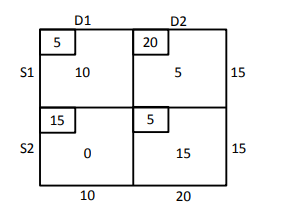
\includegraphics[width=0.75\columnwidth]{chapters/10/7/2/4/figs/fig.png}
 \end{center}
\caption{}
\label{fig:10/7/2/4Fig1}
\end{figure}
\fi

\item Find the position vector of the mid point of the vector joining the points $\vec{P}$(2, 3, 4)
and $\vec{Q}$(4, 1, –2).
\\
\solution
		\begin{enumerate}[label=\thesubsection.\arabic*,ref=\thesubsection.\theenumi]
\item Find the coordinates of the point which divides the join of $(-1,7) $ and $ (4,-3)$ in the ratio 2:3.
	\\
		\solution
	\input{chapters/10/7/2/1/section.tex}
\item Find the coordinates of the point $\vec{R}$ on the line segment joining the points $\vec{P}(-1,3)$ and $\vec{Q}(2,5)$ such that $PR=\frac{3}{5}PQ$.
\item Find the ratio in which the point $\vec{P}\brak{\frac{3}{4},\frac{5}{12}}$ divides the line segment joining the points $\vec{A}\brak{\frac{1}{2},\frac{3}{2}}$ and $ \vec{B}(2,-5)$.
\item Find the coordinates of the point which divides the line segment joining the points $(4,-3)$ and $(8,5)$ in the ratio $3:1$ internally.
\item Find the coordinates of the point $\vec{P}$ on $AD$ such that $AP : PD = 2 : 1$.
\item If the point $\vec{P} (2, 1)$ lies on the line segment joining points $\vec{A} (4, 2)$  and $ \vec{B} (8, 4)$,
then
\begin{enumerate}
	\item $AP =\frac{1}{3}{AB}$ 
\item ${AP}={PE}$
\item ${PB}=\frac{1}{3}{AB}$
\item${AP}=\frac{1}{2}{AB}$
 \end{enumerate}
\item Find the ratio in which the line segment joining the points $(-3,10)$  and  $(6,-8)$  is divided by $ (-1,6)$.
	\\
		\solution
	\input{chapters/10/7/2/4/section.tex}
\item Find the position vector of the mid point of the vector joining the points $\vec{P}$(2, 3, 4)
and $\vec{Q}$(4, 1, –2).
\\
\solution
		\input{chapters/12/10/2/16/section.tex}
\item Let $\vec{A}(4, 2), \vec{B}(6, 5)$  and $ \vec{C}(1, 4)$ be the vertices of $\triangle ABC$.
\begin{enumerate}
\item If $\vec{A}$ and  $\vec{B}$ are $(-2,-2)$ and  $(2,-4)$, respectively, find the coordinates of $\vec{P}$ such that $AP= \frac {3}{7}AB$  and $ \vec{P}$ lies on the line segment $AB$.
	\\
		\solution
	\input{chapters/10/7/2/8/section.tex}
\item Find the coordinates of the points which divide the line segment joining $A(-2,2)$  and  $\vec{B}(2,8)$ into four equal parts.
	\\
		\solution
	\input{chapters/10/7/2/9/section.tex}
\item In what ratio does the point $(-4,6)$ divide the line segment joining the points $\vec{A}(-6,0)$ and $\vec{B}(3,-8)$?
\item Given that $\vec{P}(3,2,-4), \vec{Q}(5,4,-6)$ and $\vec{R}(9,8,-10)$ are collinear. Find the ratio in which $\vec{Q}$ divides $PR$.
\item Points $\vec{A}(-6,10),\vec{B}(-4,6)$  and  $\vec{C}(3,-8)$ are collinear such that $AB=  \frac{2}{9}AC$.
\item The point which divides the line segment joining the points $\vec{P} (7, –6) $  and  $\vec{Q}(3, 4)$ in the 
ratio 1 : 2 internally lies in  which quadrant?
\item Find the coordinates of the points of trisection of the line segment joining $(4,-1)$  and  $(-2,3)$.
	\\
		\solution
	\input{chapters/10/7/2/2/section.tex}
\item Find the coordinates of the points which trisect the line segment joining the points $\vec{P}(4,2,-6)$ and $\vec{Q}(10,-16,6)$.
\item Find the coordinates of the points of trisection (i.e. points dividing to three equal parts) of the line segment joining the points $\vec{A}(2,-2)$ and $\vec{B}(-7,4)$.
\item Point $\vec{P}(5,-3)$ is one of the two points of trisection of line segment joining the points $\vec{A}(7,-2)$ and $\vec{B}(1,-5)$
\item Find the position vector of a point $\vec{R}$ which divides the line joining two points $\vec{P}$
and $\vec{Q}$ whose position vectors are $\hat{i}+2\hat{j}-\hat{k}$ and $-\hat{i}+\hat{j}+\hat{k}$ respectively, in the
ratio 2 : 1
\begin{enumerate}
    \item  internally
    \item  externally
\end{enumerate}
%\solution
%		\input{chapters/12/10/2/15/section.tex}
\item Find the coordinates of the point which divides the line segment joining the points which divides the line segment joining  the points $(-2,3,5)$ and $(1,-4,6)$ in the ratio 
\begin{enumerate}
\item $2:3$ internally,
\item $2:3$ externally
\end{enumerate}
\item Find the coordinates of the point which divides the line segment joining the points $(1,-2,3)$ and $(3,4,-5)$ in the ratio $2:3$
\begin{enumerate}
\item internally, and
\item externally
\end{enumerate}
\item Consider two points $\vec{P}$ and $\vec{Q}$ with position vectors $\overrightarrow{OP} = 3\overrightarrow{a}-2\overrightarrow{b}$ and $\overrightarrow{OQ}=\overrightarrow{a}+\overrightarrow{b}$. Find the position vector of a point $\vec{R}$ which divides the line joining $\vec{P}$ and $\vec{Q}$ in the ratio $2:1$, 
\begin{enumerate}
\item internally, and 
\item externally.
\end{enumerate}
\item The median from $\vec{A}$ meets $BC$ at $\vec{D}$. Find the coordinates of the point $\vec{D}$.
\item Find the coordinates of points $\vec{Q}$ and $\vec{R}$ on medians $BE$ and $CF$ respectively such that $BQ : QE = 2 : 1$  and  $CR : RF = 2 : 1$.
\item What do you observe?
\item If $\vec{A}, \vec{B}$ and $\vec{C}$  are the vertices of $\triangle ABC$, find the coordinates of the centroid of the triangle.
\end{enumerate}
\solution
	\input{chapters/10/7/4/7/section.tex}
\item If $\vec{P}(9a-2,-b)$ divides line segment joining $\vec{A}(3a+1,-3)$ and $\vec{B}(8a,5)$ in the ratio 3:1, find the values of $a$ and $b$.
\item Find the position vector of a point $\vec{R}$ which divides the line joining two points $\vec{P}$ and $\vec{Q}$ whose position vectors are $2\vec{a}+\vec{b}$ and $\vec{a}-3\vec{b}$ externally in the ratio $1:2$.
\item The position vector of the point which divides the join of points 2$\vec{a}$-3$\vec{b}$ $\text{and}$ $\vec{a}+\vec{b}$ in the ratio 3:1 is \rule{1cm}{0.1pt}.
\item If $\vec{a}$ and $\vec{b}$ are the postion vectors of $\vec{A}$ and $\vec{B}$, respectively, find the position vector of a point $\vec{C}$ in $BA$ produced such that $BC=1.5BA$.
\item Find the position vector of a point $\vec{R}$ which divides the line joining two points $\vec{P}$ and $\vec{Q}$ whose position vectors are $(2\vec{a}+\vec{b})$ and $(\vec{a}-3\vec{b})$
externally in the ratio 1 : 2. Also, show that $\vec{P}$ is the mid point of the line segment $RQ$.
\end{enumerate}

\item Let $\vec{A}(4, 2), \vec{B}(6, 5)$  and $ \vec{C}(1, 4)$ be the vertices of $\triangle ABC$.
\begin{enumerate}
\item If $\vec{A}$ and  $\vec{B}$ are $(-2,-2)$ and  $(2,-4)$, respectively, find the coordinates of $\vec{P}$ such that $AP= \frac {3}{7}AB$  and $ \vec{P}$ lies on the line segment $AB$.
	\\
		\solution
	\begin{enumerate}[label=\thesubsection.\arabic*,ref=\thesubsection.\theenumi]
\item Find the coordinates of the point which divides the join of $(-1,7) $ and $ (4,-3)$ in the ratio 2:3.
	\\
		\solution
	\input{chapters/10/7/2/1/section.tex}
\item Find the coordinates of the point $\vec{R}$ on the line segment joining the points $\vec{P}(-1,3)$ and $\vec{Q}(2,5)$ such that $PR=\frac{3}{5}PQ$.
\item Find the ratio in which the point $\vec{P}\brak{\frac{3}{4},\frac{5}{12}}$ divides the line segment joining the points $\vec{A}\brak{\frac{1}{2},\frac{3}{2}}$ and $ \vec{B}(2,-5)$.
\item Find the coordinates of the point which divides the line segment joining the points $(4,-3)$ and $(8,5)$ in the ratio $3:1$ internally.
\item Find the coordinates of the point $\vec{P}$ on $AD$ such that $AP : PD = 2 : 1$.
\item If the point $\vec{P} (2, 1)$ lies on the line segment joining points $\vec{A} (4, 2)$  and $ \vec{B} (8, 4)$,
then
\begin{enumerate}
	\item $AP =\frac{1}{3}{AB}$ 
\item ${AP}={PE}$
\item ${PB}=\frac{1}{3}{AB}$
\item${AP}=\frac{1}{2}{AB}$
 \end{enumerate}
\item Find the ratio in which the line segment joining the points $(-3,10)$  and  $(6,-8)$  is divided by $ (-1,6)$.
	\\
		\solution
	\input{chapters/10/7/2/4/section.tex}
\item Find the position vector of the mid point of the vector joining the points $\vec{P}$(2, 3, 4)
and $\vec{Q}$(4, 1, –2).
\\
\solution
		\input{chapters/12/10/2/16/section.tex}
\item Let $\vec{A}(4, 2), \vec{B}(6, 5)$  and $ \vec{C}(1, 4)$ be the vertices of $\triangle ABC$.
\begin{enumerate}
\item If $\vec{A}$ and  $\vec{B}$ are $(-2,-2)$ and  $(2,-4)$, respectively, find the coordinates of $\vec{P}$ such that $AP= \frac {3}{7}AB$  and $ \vec{P}$ lies on the line segment $AB$.
	\\
		\solution
	\input{chapters/10/7/2/8/section.tex}
\item Find the coordinates of the points which divide the line segment joining $A(-2,2)$  and  $\vec{B}(2,8)$ into four equal parts.
	\\
		\solution
	\input{chapters/10/7/2/9/section.tex}
\item In what ratio does the point $(-4,6)$ divide the line segment joining the points $\vec{A}(-6,0)$ and $\vec{B}(3,-8)$?
\item Given that $\vec{P}(3,2,-4), \vec{Q}(5,4,-6)$ and $\vec{R}(9,8,-10)$ are collinear. Find the ratio in which $\vec{Q}$ divides $PR$.
\item Points $\vec{A}(-6,10),\vec{B}(-4,6)$  and  $\vec{C}(3,-8)$ are collinear such that $AB=  \frac{2}{9}AC$.
\item The point which divides the line segment joining the points $\vec{P} (7, –6) $  and  $\vec{Q}(3, 4)$ in the 
ratio 1 : 2 internally lies in  which quadrant?
\item Find the coordinates of the points of trisection of the line segment joining $(4,-1)$  and  $(-2,3)$.
	\\
		\solution
	\input{chapters/10/7/2/2/section.tex}
\item Find the coordinates of the points which trisect the line segment joining the points $\vec{P}(4,2,-6)$ and $\vec{Q}(10,-16,6)$.
\item Find the coordinates of the points of trisection (i.e. points dividing to three equal parts) of the line segment joining the points $\vec{A}(2,-2)$ and $\vec{B}(-7,4)$.
\item Point $\vec{P}(5,-3)$ is one of the two points of trisection of line segment joining the points $\vec{A}(7,-2)$ and $\vec{B}(1,-5)$
\item Find the position vector of a point $\vec{R}$ which divides the line joining two points $\vec{P}$
and $\vec{Q}$ whose position vectors are $\hat{i}+2\hat{j}-\hat{k}$ and $-\hat{i}+\hat{j}+\hat{k}$ respectively, in the
ratio 2 : 1
\begin{enumerate}
    \item  internally
    \item  externally
\end{enumerate}
%\solution
%		\input{chapters/12/10/2/15/section.tex}
\item Find the coordinates of the point which divides the line segment joining the points which divides the line segment joining  the points $(-2,3,5)$ and $(1,-4,6)$ in the ratio 
\begin{enumerate}
\item $2:3$ internally,
\item $2:3$ externally
\end{enumerate}
\item Find the coordinates of the point which divides the line segment joining the points $(1,-2,3)$ and $(3,4,-5)$ in the ratio $2:3$
\begin{enumerate}
\item internally, and
\item externally
\end{enumerate}
\item Consider two points $\vec{P}$ and $\vec{Q}$ with position vectors $\overrightarrow{OP} = 3\overrightarrow{a}-2\overrightarrow{b}$ and $\overrightarrow{OQ}=\overrightarrow{a}+\overrightarrow{b}$. Find the position vector of a point $\vec{R}$ which divides the line joining $\vec{P}$ and $\vec{Q}$ in the ratio $2:1$, 
\begin{enumerate}
\item internally, and 
\item externally.
\end{enumerate}
\item The median from $\vec{A}$ meets $BC$ at $\vec{D}$. Find the coordinates of the point $\vec{D}$.
\item Find the coordinates of points $\vec{Q}$ and $\vec{R}$ on medians $BE$ and $CF$ respectively such that $BQ : QE = 2 : 1$  and  $CR : RF = 2 : 1$.
\item What do you observe?
\item If $\vec{A}, \vec{B}$ and $\vec{C}$  are the vertices of $\triangle ABC$, find the coordinates of the centroid of the triangle.
\end{enumerate}
\solution
	\input{chapters/10/7/4/7/section.tex}
\item If $\vec{P}(9a-2,-b)$ divides line segment joining $\vec{A}(3a+1,-3)$ and $\vec{B}(8a,5)$ in the ratio 3:1, find the values of $a$ and $b$.
\item Find the position vector of a point $\vec{R}$ which divides the line joining two points $\vec{P}$ and $\vec{Q}$ whose position vectors are $2\vec{a}+\vec{b}$ and $\vec{a}-3\vec{b}$ externally in the ratio $1:2$.
\item The position vector of the point which divides the join of points 2$\vec{a}$-3$\vec{b}$ $\text{and}$ $\vec{a}+\vec{b}$ in the ratio 3:1 is \rule{1cm}{0.1pt}.
\item If $\vec{a}$ and $\vec{b}$ are the postion vectors of $\vec{A}$ and $\vec{B}$, respectively, find the position vector of a point $\vec{C}$ in $BA$ produced such that $BC=1.5BA$.
\item Find the position vector of a point $\vec{R}$ which divides the line joining two points $\vec{P}$ and $\vec{Q}$ whose position vectors are $(2\vec{a}+\vec{b})$ and $(\vec{a}-3\vec{b})$
externally in the ratio 1 : 2. Also, show that $\vec{P}$ is the mid point of the line segment $RQ$.
\end{enumerate}

\item Find the coordinates of the points which divide the line segment joining $A(-2,2)$  and  $\vec{B}(2,8)$ into four equal parts.
	\\
		\solution
	\begin{enumerate}[label=\thesubsection.\arabic*,ref=\thesubsection.\theenumi]
\item Find the coordinates of the point which divides the join of $(-1,7) $ and $ (4,-3)$ in the ratio 2:3.
	\\
		\solution
	\input{chapters/10/7/2/1/section.tex}
\item Find the coordinates of the point $\vec{R}$ on the line segment joining the points $\vec{P}(-1,3)$ and $\vec{Q}(2,5)$ such that $PR=\frac{3}{5}PQ$.
\item Find the ratio in which the point $\vec{P}\brak{\frac{3}{4},\frac{5}{12}}$ divides the line segment joining the points $\vec{A}\brak{\frac{1}{2},\frac{3}{2}}$ and $ \vec{B}(2,-5)$.
\item Find the coordinates of the point which divides the line segment joining the points $(4,-3)$ and $(8,5)$ in the ratio $3:1$ internally.
\item Find the coordinates of the point $\vec{P}$ on $AD$ such that $AP : PD = 2 : 1$.
\item If the point $\vec{P} (2, 1)$ lies on the line segment joining points $\vec{A} (4, 2)$  and $ \vec{B} (8, 4)$,
then
\begin{enumerate}
	\item $AP =\frac{1}{3}{AB}$ 
\item ${AP}={PE}$
\item ${PB}=\frac{1}{3}{AB}$
\item${AP}=\frac{1}{2}{AB}$
 \end{enumerate}
\item Find the ratio in which the line segment joining the points $(-3,10)$  and  $(6,-8)$  is divided by $ (-1,6)$.
	\\
		\solution
	\input{chapters/10/7/2/4/section.tex}
\item Find the position vector of the mid point of the vector joining the points $\vec{P}$(2, 3, 4)
and $\vec{Q}$(4, 1, –2).
\\
\solution
		\input{chapters/12/10/2/16/section.tex}
\item Let $\vec{A}(4, 2), \vec{B}(6, 5)$  and $ \vec{C}(1, 4)$ be the vertices of $\triangle ABC$.
\begin{enumerate}
\item If $\vec{A}$ and  $\vec{B}$ are $(-2,-2)$ and  $(2,-4)$, respectively, find the coordinates of $\vec{P}$ such that $AP= \frac {3}{7}AB$  and $ \vec{P}$ lies on the line segment $AB$.
	\\
		\solution
	\input{chapters/10/7/2/8/section.tex}
\item Find the coordinates of the points which divide the line segment joining $A(-2,2)$  and  $\vec{B}(2,8)$ into four equal parts.
	\\
		\solution
	\input{chapters/10/7/2/9/section.tex}
\item In what ratio does the point $(-4,6)$ divide the line segment joining the points $\vec{A}(-6,0)$ and $\vec{B}(3,-8)$?
\item Given that $\vec{P}(3,2,-4), \vec{Q}(5,4,-6)$ and $\vec{R}(9,8,-10)$ are collinear. Find the ratio in which $\vec{Q}$ divides $PR$.
\item Points $\vec{A}(-6,10),\vec{B}(-4,6)$  and  $\vec{C}(3,-8)$ are collinear such that $AB=  \frac{2}{9}AC$.
\item The point which divides the line segment joining the points $\vec{P} (7, –6) $  and  $\vec{Q}(3, 4)$ in the 
ratio 1 : 2 internally lies in  which quadrant?
\item Find the coordinates of the points of trisection of the line segment joining $(4,-1)$  and  $(-2,3)$.
	\\
		\solution
	\input{chapters/10/7/2/2/section.tex}
\item Find the coordinates of the points which trisect the line segment joining the points $\vec{P}(4,2,-6)$ and $\vec{Q}(10,-16,6)$.
\item Find the coordinates of the points of trisection (i.e. points dividing to three equal parts) of the line segment joining the points $\vec{A}(2,-2)$ and $\vec{B}(-7,4)$.
\item Point $\vec{P}(5,-3)$ is one of the two points of trisection of line segment joining the points $\vec{A}(7,-2)$ and $\vec{B}(1,-5)$
\item Find the position vector of a point $\vec{R}$ which divides the line joining two points $\vec{P}$
and $\vec{Q}$ whose position vectors are $\hat{i}+2\hat{j}-\hat{k}$ and $-\hat{i}+\hat{j}+\hat{k}$ respectively, in the
ratio 2 : 1
\begin{enumerate}
    \item  internally
    \item  externally
\end{enumerate}
%\solution
%		\input{chapters/12/10/2/15/section.tex}
\item Find the coordinates of the point which divides the line segment joining the points which divides the line segment joining  the points $(-2,3,5)$ and $(1,-4,6)$ in the ratio 
\begin{enumerate}
\item $2:3$ internally,
\item $2:3$ externally
\end{enumerate}
\item Find the coordinates of the point which divides the line segment joining the points $(1,-2,3)$ and $(3,4,-5)$ in the ratio $2:3$
\begin{enumerate}
\item internally, and
\item externally
\end{enumerate}
\item Consider two points $\vec{P}$ and $\vec{Q}$ with position vectors $\overrightarrow{OP} = 3\overrightarrow{a}-2\overrightarrow{b}$ and $\overrightarrow{OQ}=\overrightarrow{a}+\overrightarrow{b}$. Find the position vector of a point $\vec{R}$ which divides the line joining $\vec{P}$ and $\vec{Q}$ in the ratio $2:1$, 
\begin{enumerate}
\item internally, and 
\item externally.
\end{enumerate}
\item The median from $\vec{A}$ meets $BC$ at $\vec{D}$. Find the coordinates of the point $\vec{D}$.
\item Find the coordinates of points $\vec{Q}$ and $\vec{R}$ on medians $BE$ and $CF$ respectively such that $BQ : QE = 2 : 1$  and  $CR : RF = 2 : 1$.
\item What do you observe?
\item If $\vec{A}, \vec{B}$ and $\vec{C}$  are the vertices of $\triangle ABC$, find the coordinates of the centroid of the triangle.
\end{enumerate}
\solution
	\input{chapters/10/7/4/7/section.tex}
\item If $\vec{P}(9a-2,-b)$ divides line segment joining $\vec{A}(3a+1,-3)$ and $\vec{B}(8a,5)$ in the ratio 3:1, find the values of $a$ and $b$.
\item Find the position vector of a point $\vec{R}$ which divides the line joining two points $\vec{P}$ and $\vec{Q}$ whose position vectors are $2\vec{a}+\vec{b}$ and $\vec{a}-3\vec{b}$ externally in the ratio $1:2$.
\item The position vector of the point which divides the join of points 2$\vec{a}$-3$\vec{b}$ $\text{and}$ $\vec{a}+\vec{b}$ in the ratio 3:1 is \rule{1cm}{0.1pt}.
\item If $\vec{a}$ and $\vec{b}$ are the postion vectors of $\vec{A}$ and $\vec{B}$, respectively, find the position vector of a point $\vec{C}$ in $BA$ produced such that $BC=1.5BA$.
\item Find the position vector of a point $\vec{R}$ which divides the line joining two points $\vec{P}$ and $\vec{Q}$ whose position vectors are $(2\vec{a}+\vec{b})$ and $(\vec{a}-3\vec{b})$
externally in the ratio 1 : 2. Also, show that $\vec{P}$ is the mid point of the line segment $RQ$.
\end{enumerate}

\item In what ratio does the point $(-4,6)$ divide the line segment joining the points $\vec{A}(-6,0)$ and $\vec{B}(3,-8)$?
\item Given that $\vec{P}(3,2,-4), \vec{Q}(5,4,-6)$ and $\vec{R}(9,8,-10)$ are collinear. Find the ratio in which $\vec{Q}$ divides $PR$.
\item Points $\vec{A}(-6,10),\vec{B}(-4,6)$  and  $\vec{C}(3,-8)$ are collinear such that $AB=  \frac{2}{9}AC$.
\item The point which divides the line segment joining the points $\vec{P} (7, –6) $  and  $\vec{Q}(3, 4)$ in the 
ratio 1 : 2 internally lies in  which quadrant?
\item Find the coordinates of the points of trisection of the line segment joining $(4,-1)$  and  $(-2,3)$.
	\\
		\solution
	Using section formula,
\begin{align}
\vec{R}=\frac{1}{1+\frac{1}{2}}\brak{\myvec{4\\-1}+\frac{1}{2}\myvec{-2\\3}}
=\myvec{2\\ \frac{1}{3}}\\
\vec{S}=\frac{1}{1+\frac{2}{1}}\brak{\myvec{4\\-1}+\frac{2}{1}\myvec{-2\\3}}
=\myvec{0\\ \frac{5}{3}}
\end{align}
which are the desired points of trisection.
\iffalse
See
		\figref{fig:chapters/10/7/2/2/Figure}
\begin{figure}[H]
\centering
\includegraphics[width=0.75\columnwidth]{chapters/10/7/2/2/figs/dj.pdf}
\caption{}
		\label{fig:chapters/10/7/2/2/Figure}
\end{figure}
\fi

\item Find the coordinates of the points which trisect the line segment joining the points $\vec{P}(4,2,-6)$ and $\vec{Q}(10,-16,6)$.
\item Find the coordinates of the points of trisection (i.e. points dividing to three equal parts) of the line segment joining the points $\vec{A}(2,-2)$ and $\vec{B}(-7,4)$.
\item Point $\vec{P}(5,-3)$ is one of the two points of trisection of line segment joining the points $\vec{A}(7,-2)$ and $\vec{B}(1,-5)$
\item Find the position vector of a point $\vec{R}$ which divides the line joining two points $\vec{P}$
and $\vec{Q}$ whose position vectors are $\hat{i}+2\hat{j}-\hat{k}$ and $-\hat{i}+\hat{j}+\hat{k}$ respectively, in the
ratio 2 : 1
\begin{enumerate}
    \item  internally
    \item  externally
\end{enumerate}
%\solution
%		\begin{enumerate}[label=\thesubsection.\arabic*,ref=\thesubsection.\theenumi]
\item Find the coordinates of the point which divides the join of $(-1,7) $ and $ (4,-3)$ in the ratio 2:3.
	\\
		\solution
	\input{chapters/10/7/2/1/section.tex}
\item Find the coordinates of the point $\vec{R}$ on the line segment joining the points $\vec{P}(-1,3)$ and $\vec{Q}(2,5)$ such that $PR=\frac{3}{5}PQ$.
\item Find the ratio in which the point $\vec{P}\brak{\frac{3}{4},\frac{5}{12}}$ divides the line segment joining the points $\vec{A}\brak{\frac{1}{2},\frac{3}{2}}$ and $ \vec{B}(2,-5)$.
\item Find the coordinates of the point which divides the line segment joining the points $(4,-3)$ and $(8,5)$ in the ratio $3:1$ internally.
\item Find the coordinates of the point $\vec{P}$ on $AD$ such that $AP : PD = 2 : 1$.
\item If the point $\vec{P} (2, 1)$ lies on the line segment joining points $\vec{A} (4, 2)$  and $ \vec{B} (8, 4)$,
then
\begin{enumerate}
	\item $AP =\frac{1}{3}{AB}$ 
\item ${AP}={PE}$
\item ${PB}=\frac{1}{3}{AB}$
\item${AP}=\frac{1}{2}{AB}$
 \end{enumerate}
\item Find the ratio in which the line segment joining the points $(-3,10)$  and  $(6,-8)$  is divided by $ (-1,6)$.
	\\
		\solution
	\input{chapters/10/7/2/4/section.tex}
\item Find the position vector of the mid point of the vector joining the points $\vec{P}$(2, 3, 4)
and $\vec{Q}$(4, 1, –2).
\\
\solution
		\input{chapters/12/10/2/16/section.tex}
\item Let $\vec{A}(4, 2), \vec{B}(6, 5)$  and $ \vec{C}(1, 4)$ be the vertices of $\triangle ABC$.
\begin{enumerate}
\item If $\vec{A}$ and  $\vec{B}$ are $(-2,-2)$ and  $(2,-4)$, respectively, find the coordinates of $\vec{P}$ such that $AP= \frac {3}{7}AB$  and $ \vec{P}$ lies on the line segment $AB$.
	\\
		\solution
	\input{chapters/10/7/2/8/section.tex}
\item Find the coordinates of the points which divide the line segment joining $A(-2,2)$  and  $\vec{B}(2,8)$ into four equal parts.
	\\
		\solution
	\input{chapters/10/7/2/9/section.tex}
\item In what ratio does the point $(-4,6)$ divide the line segment joining the points $\vec{A}(-6,0)$ and $\vec{B}(3,-8)$?
\item Given that $\vec{P}(3,2,-4), \vec{Q}(5,4,-6)$ and $\vec{R}(9,8,-10)$ are collinear. Find the ratio in which $\vec{Q}$ divides $PR$.
\item Points $\vec{A}(-6,10),\vec{B}(-4,6)$  and  $\vec{C}(3,-8)$ are collinear such that $AB=  \frac{2}{9}AC$.
\item The point which divides the line segment joining the points $\vec{P} (7, –6) $  and  $\vec{Q}(3, 4)$ in the 
ratio 1 : 2 internally lies in  which quadrant?
\item Find the coordinates of the points of trisection of the line segment joining $(4,-1)$  and  $(-2,3)$.
	\\
		\solution
	\input{chapters/10/7/2/2/section.tex}
\item Find the coordinates of the points which trisect the line segment joining the points $\vec{P}(4,2,-6)$ and $\vec{Q}(10,-16,6)$.
\item Find the coordinates of the points of trisection (i.e. points dividing to three equal parts) of the line segment joining the points $\vec{A}(2,-2)$ and $\vec{B}(-7,4)$.
\item Point $\vec{P}(5,-3)$ is one of the two points of trisection of line segment joining the points $\vec{A}(7,-2)$ and $\vec{B}(1,-5)$
\item Find the position vector of a point $\vec{R}$ which divides the line joining two points $\vec{P}$
and $\vec{Q}$ whose position vectors are $\hat{i}+2\hat{j}-\hat{k}$ and $-\hat{i}+\hat{j}+\hat{k}$ respectively, in the
ratio 2 : 1
\begin{enumerate}
    \item  internally
    \item  externally
\end{enumerate}
%\solution
%		\input{chapters/12/10/2/15/section.tex}
\item Find the coordinates of the point which divides the line segment joining the points which divides the line segment joining  the points $(-2,3,5)$ and $(1,-4,6)$ in the ratio 
\begin{enumerate}
\item $2:3$ internally,
\item $2:3$ externally
\end{enumerate}
\item Find the coordinates of the point which divides the line segment joining the points $(1,-2,3)$ and $(3,4,-5)$ in the ratio $2:3$
\begin{enumerate}
\item internally, and
\item externally
\end{enumerate}
\item Consider two points $\vec{P}$ and $\vec{Q}$ with position vectors $\overrightarrow{OP} = 3\overrightarrow{a}-2\overrightarrow{b}$ and $\overrightarrow{OQ}=\overrightarrow{a}+\overrightarrow{b}$. Find the position vector of a point $\vec{R}$ which divides the line joining $\vec{P}$ and $\vec{Q}$ in the ratio $2:1$, 
\begin{enumerate}
\item internally, and 
\item externally.
\end{enumerate}
\item The median from $\vec{A}$ meets $BC$ at $\vec{D}$. Find the coordinates of the point $\vec{D}$.
\item Find the coordinates of points $\vec{Q}$ and $\vec{R}$ on medians $BE$ and $CF$ respectively such that $BQ : QE = 2 : 1$  and  $CR : RF = 2 : 1$.
\item What do you observe?
\item If $\vec{A}, \vec{B}$ and $\vec{C}$  are the vertices of $\triangle ABC$, find the coordinates of the centroid of the triangle.
\end{enumerate}
\solution
	\input{chapters/10/7/4/7/section.tex}
\item If $\vec{P}(9a-2,-b)$ divides line segment joining $\vec{A}(3a+1,-3)$ and $\vec{B}(8a,5)$ in the ratio 3:1, find the values of $a$ and $b$.
\item Find the position vector of a point $\vec{R}$ which divides the line joining two points $\vec{P}$ and $\vec{Q}$ whose position vectors are $2\vec{a}+\vec{b}$ and $\vec{a}-3\vec{b}$ externally in the ratio $1:2$.
\item The position vector of the point which divides the join of points 2$\vec{a}$-3$\vec{b}$ $\text{and}$ $\vec{a}+\vec{b}$ in the ratio 3:1 is \rule{1cm}{0.1pt}.
\item If $\vec{a}$ and $\vec{b}$ are the postion vectors of $\vec{A}$ and $\vec{B}$, respectively, find the position vector of a point $\vec{C}$ in $BA$ produced such that $BC=1.5BA$.
\item Find the position vector of a point $\vec{R}$ which divides the line joining two points $\vec{P}$ and $\vec{Q}$ whose position vectors are $(2\vec{a}+\vec{b})$ and $(\vec{a}-3\vec{b})$
externally in the ratio 1 : 2. Also, show that $\vec{P}$ is the mid point of the line segment $RQ$.
\end{enumerate}

\item Find the coordinates of the point which divides the line segment joining the points which divides the line segment joining  the points $(-2,3,5)$ and $(1,-4,6)$ in the ratio 
\begin{enumerate}
\item $2:3$ internally,
\item $2:3$ externally
\end{enumerate}
\item Find the coordinates of the point which divides the line segment joining the points $(1,-2,3)$ and $(3,4,-5)$ in the ratio $2:3$
\begin{enumerate}
\item internally, and
\item externally
\end{enumerate}
\item Consider two points $\vec{P}$ and $\vec{Q}$ with position vectors $\overrightarrow{OP} = 3\overrightarrow{a}-2\overrightarrow{b}$ and $\overrightarrow{OQ}=\overrightarrow{a}+\overrightarrow{b}$. Find the position vector of a point $\vec{R}$ which divides the line joining $\vec{P}$ and $\vec{Q}$ in the ratio $2:1$, 
\begin{enumerate}
\item internally, and 
\item externally.
\end{enumerate}
\item The median from $\vec{A}$ meets $BC$ at $\vec{D}$. Find the coordinates of the point $\vec{D}$.
\item Find the coordinates of points $\vec{Q}$ and $\vec{R}$ on medians $BE$ and $CF$ respectively such that $BQ : QE = 2 : 1$  and  $CR : RF = 2 : 1$.
\item What do you observe?
\item If $\vec{A}, \vec{B}$ and $\vec{C}$  are the vertices of $\triangle ABC$, find the coordinates of the centroid of the triangle.
\end{enumerate}
\solution
	\begin{enumerate}[label=\thesubsection.\arabic*,ref=\thesubsection.\theenumi]
\item Find the coordinates of the point which divides the join of $(-1,7) $ and $ (4,-3)$ in the ratio 2:3.
	\\
		\solution
	\input{chapters/10/7/2/1/section.tex}
\item Find the coordinates of the point $\vec{R}$ on the line segment joining the points $\vec{P}(-1,3)$ and $\vec{Q}(2,5)$ such that $PR=\frac{3}{5}PQ$.
\item Find the ratio in which the point $\vec{P}\brak{\frac{3}{4},\frac{5}{12}}$ divides the line segment joining the points $\vec{A}\brak{\frac{1}{2},\frac{3}{2}}$ and $ \vec{B}(2,-5)$.
\item Find the coordinates of the point which divides the line segment joining the points $(4,-3)$ and $(8,5)$ in the ratio $3:1$ internally.
\item Find the coordinates of the point $\vec{P}$ on $AD$ such that $AP : PD = 2 : 1$.
\item If the point $\vec{P} (2, 1)$ lies on the line segment joining points $\vec{A} (4, 2)$  and $ \vec{B} (8, 4)$,
then
\begin{enumerate}
	\item $AP =\frac{1}{3}{AB}$ 
\item ${AP}={PE}$
\item ${PB}=\frac{1}{3}{AB}$
\item${AP}=\frac{1}{2}{AB}$
 \end{enumerate}
\item Find the ratio in which the line segment joining the points $(-3,10)$  and  $(6,-8)$  is divided by $ (-1,6)$.
	\\
		\solution
	\input{chapters/10/7/2/4/section.tex}
\item Find the position vector of the mid point of the vector joining the points $\vec{P}$(2, 3, 4)
and $\vec{Q}$(4, 1, –2).
\\
\solution
		\input{chapters/12/10/2/16/section.tex}
\item Let $\vec{A}(4, 2), \vec{B}(6, 5)$  and $ \vec{C}(1, 4)$ be the vertices of $\triangle ABC$.
\begin{enumerate}
\item If $\vec{A}$ and  $\vec{B}$ are $(-2,-2)$ and  $(2,-4)$, respectively, find the coordinates of $\vec{P}$ such that $AP= \frac {3}{7}AB$  and $ \vec{P}$ lies on the line segment $AB$.
	\\
		\solution
	\input{chapters/10/7/2/8/section.tex}
\item Find the coordinates of the points which divide the line segment joining $A(-2,2)$  and  $\vec{B}(2,8)$ into four equal parts.
	\\
		\solution
	\input{chapters/10/7/2/9/section.tex}
\item In what ratio does the point $(-4,6)$ divide the line segment joining the points $\vec{A}(-6,0)$ and $\vec{B}(3,-8)$?
\item Given that $\vec{P}(3,2,-4), \vec{Q}(5,4,-6)$ and $\vec{R}(9,8,-10)$ are collinear. Find the ratio in which $\vec{Q}$ divides $PR$.
\item Points $\vec{A}(-6,10),\vec{B}(-4,6)$  and  $\vec{C}(3,-8)$ are collinear such that $AB=  \frac{2}{9}AC$.
\item The point which divides the line segment joining the points $\vec{P} (7, –6) $  and  $\vec{Q}(3, 4)$ in the 
ratio 1 : 2 internally lies in  which quadrant?
\item Find the coordinates of the points of trisection of the line segment joining $(4,-1)$  and  $(-2,3)$.
	\\
		\solution
	\input{chapters/10/7/2/2/section.tex}
\item Find the coordinates of the points which trisect the line segment joining the points $\vec{P}(4,2,-6)$ and $\vec{Q}(10,-16,6)$.
\item Find the coordinates of the points of trisection (i.e. points dividing to three equal parts) of the line segment joining the points $\vec{A}(2,-2)$ and $\vec{B}(-7,4)$.
\item Point $\vec{P}(5,-3)$ is one of the two points of trisection of line segment joining the points $\vec{A}(7,-2)$ and $\vec{B}(1,-5)$
\item Find the position vector of a point $\vec{R}$ which divides the line joining two points $\vec{P}$
and $\vec{Q}$ whose position vectors are $\hat{i}+2\hat{j}-\hat{k}$ and $-\hat{i}+\hat{j}+\hat{k}$ respectively, in the
ratio 2 : 1
\begin{enumerate}
    \item  internally
    \item  externally
\end{enumerate}
%\solution
%		\input{chapters/12/10/2/15/section.tex}
\item Find the coordinates of the point which divides the line segment joining the points which divides the line segment joining  the points $(-2,3,5)$ and $(1,-4,6)$ in the ratio 
\begin{enumerate}
\item $2:3$ internally,
\item $2:3$ externally
\end{enumerate}
\item Find the coordinates of the point which divides the line segment joining the points $(1,-2,3)$ and $(3,4,-5)$ in the ratio $2:3$
\begin{enumerate}
\item internally, and
\item externally
\end{enumerate}
\item Consider two points $\vec{P}$ and $\vec{Q}$ with position vectors $\overrightarrow{OP} = 3\overrightarrow{a}-2\overrightarrow{b}$ and $\overrightarrow{OQ}=\overrightarrow{a}+\overrightarrow{b}$. Find the position vector of a point $\vec{R}$ which divides the line joining $\vec{P}$ and $\vec{Q}$ in the ratio $2:1$, 
\begin{enumerate}
\item internally, and 
\item externally.
\end{enumerate}
\item The median from $\vec{A}$ meets $BC$ at $\vec{D}$. Find the coordinates of the point $\vec{D}$.
\item Find the coordinates of points $\vec{Q}$ and $\vec{R}$ on medians $BE$ and $CF$ respectively such that $BQ : QE = 2 : 1$  and  $CR : RF = 2 : 1$.
\item What do you observe?
\item If $\vec{A}, \vec{B}$ and $\vec{C}$  are the vertices of $\triangle ABC$, find the coordinates of the centroid of the triangle.
\end{enumerate}
\solution
	\input{chapters/10/7/4/7/section.tex}
\item If $\vec{P}(9a-2,-b)$ divides line segment joining $\vec{A}(3a+1,-3)$ and $\vec{B}(8a,5)$ in the ratio 3:1, find the values of $a$ and $b$.
\item Find the position vector of a point $\vec{R}$ which divides the line joining two points $\vec{P}$ and $\vec{Q}$ whose position vectors are $2\vec{a}+\vec{b}$ and $\vec{a}-3\vec{b}$ externally in the ratio $1:2$.
\item The position vector of the point which divides the join of points 2$\vec{a}$-3$\vec{b}$ $\text{and}$ $\vec{a}+\vec{b}$ in the ratio 3:1 is \rule{1cm}{0.1pt}.
\item If $\vec{a}$ and $\vec{b}$ are the postion vectors of $\vec{A}$ and $\vec{B}$, respectively, find the position vector of a point $\vec{C}$ in $BA$ produced such that $BC=1.5BA$.
\item Find the position vector of a point $\vec{R}$ which divides the line joining two points $\vec{P}$ and $\vec{Q}$ whose position vectors are $(2\vec{a}+\vec{b})$ and $(\vec{a}-3\vec{b})$
externally in the ratio 1 : 2. Also, show that $\vec{P}$ is the mid point of the line segment $RQ$.
\end{enumerate}

\item If $\vec{P}(9a-2,-b)$ divides line segment joining $\vec{A}(3a+1,-3)$ and $\vec{B}(8a,5)$ in the ratio 3:1, find the values of $a$ and $b$.
\item Find the position vector of a point $\vec{R}$ which divides the line joining two points $\vec{P}$ and $\vec{Q}$ whose position vectors are $2\vec{a}+\vec{b}$ and $\vec{a}-3\vec{b}$ externally in the ratio $1:2$.
\item The position vector of the point which divides the join of points 2$\vec{a}$-3$\vec{b}$ $\text{and}$ $\vec{a}+\vec{b}$ in the ratio 3:1 is \rule{1cm}{0.1pt}.
\item If $\vec{a}$ and $\vec{b}$ are the postion vectors of $\vec{A}$ and $\vec{B}$, respectively, find the position vector of a point $\vec{C}$ in $BA$ produced such that $BC=1.5BA$.
\item Find the position vector of a point $\vec{R}$ which divides the line joining two points $\vec{P}$ and $\vec{Q}$ whose position vectors are $(2\vec{a}+\vec{b})$ and $(\vec{a}-3\vec{b})$
externally in the ratio 1 : 2. Also, show that $\vec{P}$ is the mid point of the line segment $RQ$.
\end{enumerate}

\item Find the coordinates of the point $\vec{R}$ on the line segment joining the points $\vec{P}(-1,3)$ and $\vec{Q}(2,5)$ such that $PR=\frac{3}{5}PQ$.
\item Find the ratio in which the point $\vec{P}\brak{\frac{3}{4},\frac{5}{12}}$ divides the line segment joining the points $\vec{A}\brak{\frac{1}{2},\frac{3}{2}}$ and $ \vec{B}(2,-5)$.
\item Find the coordinates of the point which divides the line segment joining the points $(4,-3)$ and $(8,5)$ in the ratio $3:1$ internally.
\item Find the coordinates of the point $\vec{P}$ on $AD$ such that $AP : PD = 2 : 1$.
\item If the point $\vec{P} (2, 1)$ lies on the line segment joining points $\vec{A} (4, 2)$  and $ \vec{B} (8, 4)$,
then
\begin{enumerate}
	\item $AP =\frac{1}{3}{AB}$ 
\item ${AP}={PE}$
\item ${PB}=\frac{1}{3}{AB}$
\item${AP}=\frac{1}{2}{AB}$
 \end{enumerate}
\item Find the ratio in which the line segment joining the points $(-3,10)$  and  $(6,-8)$  is divided by $ (-1,6)$.
	\\
		\solution
	\iffalse
Using section formula,
\begin{align}
         \myvec{-1\\6} &=\frac{{\myvec{-3\\10}+k\myvec{6\\-8}}}{1+k}\\
	 \implies 7k\myvec{1 \\ -2} &= 2\myvec{1 \\ -2}
	 \\
	 \text{or, } k &= \frac{2}{7}.
\end{align}
\fi
In 
			\eqref{eq:section_formula-k}, substituting
			\begin{align}
				\vec{B} &= \myvec{-3\\10}, \vec{C} = \myvec{6\\-8}, \vec{D} = \myvec{-1\\6},
				\\
				k &= \frac{\myvec{-2 & 4}\myvec{-7 \\ 14}}{\norm{\myvec{-7 \\ 14}}^2} = \frac{2}{7}
			\end{align}
\iffalse
See \figref{fig:10/7/2/4Fig1}.
\begin{figure}[H]
 \begin{center}
  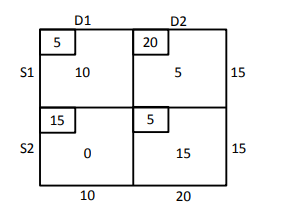
\includegraphics[width=0.75\columnwidth]{chapters/10/7/2/4/figs/fig.png}
 \end{center}
\caption{}
\label{fig:10/7/2/4Fig1}
\end{figure}
\fi

\item Find the position vector of the mid point of the vector joining the points $\vec{P}$(2, 3, 4)
and $\vec{Q}$(4, 1, –2).
\\
\solution
		\begin{enumerate}[label=\thesubsection.\arabic*,ref=\thesubsection.\theenumi]
\item Find the coordinates of the point which divides the join of $(-1,7) $ and $ (4,-3)$ in the ratio 2:3.
	\\
		\solution
	\begin{enumerate}[label=\thesubsection.\arabic*,ref=\thesubsection.\theenumi]
\item Find the coordinates of the point which divides the join of $(-1,7) $ and $ (4,-3)$ in the ratio 2:3.
	\\
		\solution
	\input{chapters/10/7/2/1/section.tex}
\item Find the coordinates of the point $\vec{R}$ on the line segment joining the points $\vec{P}(-1,3)$ and $\vec{Q}(2,5)$ such that $PR=\frac{3}{5}PQ$.
\item Find the ratio in which the point $\vec{P}\brak{\frac{3}{4},\frac{5}{12}}$ divides the line segment joining the points $\vec{A}\brak{\frac{1}{2},\frac{3}{2}}$ and $ \vec{B}(2,-5)$.
\item Find the coordinates of the point which divides the line segment joining the points $(4,-3)$ and $(8,5)$ in the ratio $3:1$ internally.
\item Find the coordinates of the point $\vec{P}$ on $AD$ such that $AP : PD = 2 : 1$.
\item If the point $\vec{P} (2, 1)$ lies on the line segment joining points $\vec{A} (4, 2)$  and $ \vec{B} (8, 4)$,
then
\begin{enumerate}
	\item $AP =\frac{1}{3}{AB}$ 
\item ${AP}={PE}$
\item ${PB}=\frac{1}{3}{AB}$
\item${AP}=\frac{1}{2}{AB}$
 \end{enumerate}
\item Find the ratio in which the line segment joining the points $(-3,10)$  and  $(6,-8)$  is divided by $ (-1,6)$.
	\\
		\solution
	\input{chapters/10/7/2/4/section.tex}
\item Find the position vector of the mid point of the vector joining the points $\vec{P}$(2, 3, 4)
and $\vec{Q}$(4, 1, –2).
\\
\solution
		\input{chapters/12/10/2/16/section.tex}
\item Let $\vec{A}(4, 2), \vec{B}(6, 5)$  and $ \vec{C}(1, 4)$ be the vertices of $\triangle ABC$.
\begin{enumerate}
\item If $\vec{A}$ and  $\vec{B}$ are $(-2,-2)$ and  $(2,-4)$, respectively, find the coordinates of $\vec{P}$ such that $AP= \frac {3}{7}AB$  and $ \vec{P}$ lies on the line segment $AB$.
	\\
		\solution
	\input{chapters/10/7/2/8/section.tex}
\item Find the coordinates of the points which divide the line segment joining $A(-2,2)$  and  $\vec{B}(2,8)$ into four equal parts.
	\\
		\solution
	\input{chapters/10/7/2/9/section.tex}
\item In what ratio does the point $(-4,6)$ divide the line segment joining the points $\vec{A}(-6,0)$ and $\vec{B}(3,-8)$?
\item Given that $\vec{P}(3,2,-4), \vec{Q}(5,4,-6)$ and $\vec{R}(9,8,-10)$ are collinear. Find the ratio in which $\vec{Q}$ divides $PR$.
\item Points $\vec{A}(-6,10),\vec{B}(-4,6)$  and  $\vec{C}(3,-8)$ are collinear such that $AB=  \frac{2}{9}AC$.
\item The point which divides the line segment joining the points $\vec{P} (7, –6) $  and  $\vec{Q}(3, 4)$ in the 
ratio 1 : 2 internally lies in  which quadrant?
\item Find the coordinates of the points of trisection of the line segment joining $(4,-1)$  and  $(-2,3)$.
	\\
		\solution
	\input{chapters/10/7/2/2/section.tex}
\item Find the coordinates of the points which trisect the line segment joining the points $\vec{P}(4,2,-6)$ and $\vec{Q}(10,-16,6)$.
\item Find the coordinates of the points of trisection (i.e. points dividing to three equal parts) of the line segment joining the points $\vec{A}(2,-2)$ and $\vec{B}(-7,4)$.
\item Point $\vec{P}(5,-3)$ is one of the two points of trisection of line segment joining the points $\vec{A}(7,-2)$ and $\vec{B}(1,-5)$
\item Find the position vector of a point $\vec{R}$ which divides the line joining two points $\vec{P}$
and $\vec{Q}$ whose position vectors are $\hat{i}+2\hat{j}-\hat{k}$ and $-\hat{i}+\hat{j}+\hat{k}$ respectively, in the
ratio 2 : 1
\begin{enumerate}
    \item  internally
    \item  externally
\end{enumerate}
%\solution
%		\input{chapters/12/10/2/15/section.tex}
\item Find the coordinates of the point which divides the line segment joining the points which divides the line segment joining  the points $(-2,3,5)$ and $(1,-4,6)$ in the ratio 
\begin{enumerate}
\item $2:3$ internally,
\item $2:3$ externally
\end{enumerate}
\item Find the coordinates of the point which divides the line segment joining the points $(1,-2,3)$ and $(3,4,-5)$ in the ratio $2:3$
\begin{enumerate}
\item internally, and
\item externally
\end{enumerate}
\item Consider two points $\vec{P}$ and $\vec{Q}$ with position vectors $\overrightarrow{OP} = 3\overrightarrow{a}-2\overrightarrow{b}$ and $\overrightarrow{OQ}=\overrightarrow{a}+\overrightarrow{b}$. Find the position vector of a point $\vec{R}$ which divides the line joining $\vec{P}$ and $\vec{Q}$ in the ratio $2:1$, 
\begin{enumerate}
\item internally, and 
\item externally.
\end{enumerate}
\item The median from $\vec{A}$ meets $BC$ at $\vec{D}$. Find the coordinates of the point $\vec{D}$.
\item Find the coordinates of points $\vec{Q}$ and $\vec{R}$ on medians $BE$ and $CF$ respectively such that $BQ : QE = 2 : 1$  and  $CR : RF = 2 : 1$.
\item What do you observe?
\item If $\vec{A}, \vec{B}$ and $\vec{C}$  are the vertices of $\triangle ABC$, find the coordinates of the centroid of the triangle.
\end{enumerate}
\solution
	\input{chapters/10/7/4/7/section.tex}
\item If $\vec{P}(9a-2,-b)$ divides line segment joining $\vec{A}(3a+1,-3)$ and $\vec{B}(8a,5)$ in the ratio 3:1, find the values of $a$ and $b$.
\item Find the position vector of a point $\vec{R}$ which divides the line joining two points $\vec{P}$ and $\vec{Q}$ whose position vectors are $2\vec{a}+\vec{b}$ and $\vec{a}-3\vec{b}$ externally in the ratio $1:2$.
\item The position vector of the point which divides the join of points 2$\vec{a}$-3$\vec{b}$ $\text{and}$ $\vec{a}+\vec{b}$ in the ratio 3:1 is \rule{1cm}{0.1pt}.
\item If $\vec{a}$ and $\vec{b}$ are the postion vectors of $\vec{A}$ and $\vec{B}$, respectively, find the position vector of a point $\vec{C}$ in $BA$ produced such that $BC=1.5BA$.
\item Find the position vector of a point $\vec{R}$ which divides the line joining two points $\vec{P}$ and $\vec{Q}$ whose position vectors are $(2\vec{a}+\vec{b})$ and $(\vec{a}-3\vec{b})$
externally in the ratio 1 : 2. Also, show that $\vec{P}$ is the mid point of the line segment $RQ$.
\end{enumerate}

\item Find the coordinates of the point $\vec{R}$ on the line segment joining the points $\vec{P}(-1,3)$ and $\vec{Q}(2,5)$ such that $PR=\frac{3}{5}PQ$.
\item Find the ratio in which the point $\vec{P}\brak{\frac{3}{4},\frac{5}{12}}$ divides the line segment joining the points $\vec{A}\brak{\frac{1}{2},\frac{3}{2}}$ and $ \vec{B}(2,-5)$.
\item Find the coordinates of the point which divides the line segment joining the points $(4,-3)$ and $(8,5)$ in the ratio $3:1$ internally.
\item Find the coordinates of the point $\vec{P}$ on $AD$ such that $AP : PD = 2 : 1$.
\item If the point $\vec{P} (2, 1)$ lies on the line segment joining points $\vec{A} (4, 2)$  and $ \vec{B} (8, 4)$,
then
\begin{enumerate}
	\item $AP =\frac{1}{3}{AB}$ 
\item ${AP}={PE}$
\item ${PB}=\frac{1}{3}{AB}$
\item${AP}=\frac{1}{2}{AB}$
 \end{enumerate}
\item Find the ratio in which the line segment joining the points $(-3,10)$  and  $(6,-8)$  is divided by $ (-1,6)$.
	\\
		\solution
	\iffalse
Using section formula,
\begin{align}
         \myvec{-1\\6} &=\frac{{\myvec{-3\\10}+k\myvec{6\\-8}}}{1+k}\\
	 \implies 7k\myvec{1 \\ -2} &= 2\myvec{1 \\ -2}
	 \\
	 \text{or, } k &= \frac{2}{7}.
\end{align}
\fi
In 
			\eqref{eq:section_formula-k}, substituting
			\begin{align}
				\vec{B} &= \myvec{-3\\10}, \vec{C} = \myvec{6\\-8}, \vec{D} = \myvec{-1\\6},
				\\
				k &= \frac{\myvec{-2 & 4}\myvec{-7 \\ 14}}{\norm{\myvec{-7 \\ 14}}^2} = \frac{2}{7}
			\end{align}
\iffalse
See \figref{fig:10/7/2/4Fig1}.
\begin{figure}[H]
 \begin{center}
  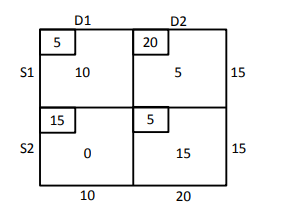
\includegraphics[width=0.75\columnwidth]{chapters/10/7/2/4/figs/fig.png}
 \end{center}
\caption{}
\label{fig:10/7/2/4Fig1}
\end{figure}
\fi

\item Find the position vector of the mid point of the vector joining the points $\vec{P}$(2, 3, 4)
and $\vec{Q}$(4, 1, –2).
\\
\solution
		\begin{enumerate}[label=\thesubsection.\arabic*,ref=\thesubsection.\theenumi]
\item Find the coordinates of the point which divides the join of $(-1,7) $ and $ (4,-3)$ in the ratio 2:3.
	\\
		\solution
	\input{chapters/10/7/2/1/section.tex}
\item Find the coordinates of the point $\vec{R}$ on the line segment joining the points $\vec{P}(-1,3)$ and $\vec{Q}(2,5)$ such that $PR=\frac{3}{5}PQ$.
\item Find the ratio in which the point $\vec{P}\brak{\frac{3}{4},\frac{5}{12}}$ divides the line segment joining the points $\vec{A}\brak{\frac{1}{2},\frac{3}{2}}$ and $ \vec{B}(2,-5)$.
\item Find the coordinates of the point which divides the line segment joining the points $(4,-3)$ and $(8,5)$ in the ratio $3:1$ internally.
\item Find the coordinates of the point $\vec{P}$ on $AD$ such that $AP : PD = 2 : 1$.
\item If the point $\vec{P} (2, 1)$ lies on the line segment joining points $\vec{A} (4, 2)$  and $ \vec{B} (8, 4)$,
then
\begin{enumerate}
	\item $AP =\frac{1}{3}{AB}$ 
\item ${AP}={PE}$
\item ${PB}=\frac{1}{3}{AB}$
\item${AP}=\frac{1}{2}{AB}$
 \end{enumerate}
\item Find the ratio in which the line segment joining the points $(-3,10)$  and  $(6,-8)$  is divided by $ (-1,6)$.
	\\
		\solution
	\input{chapters/10/7/2/4/section.tex}
\item Find the position vector of the mid point of the vector joining the points $\vec{P}$(2, 3, 4)
and $\vec{Q}$(4, 1, –2).
\\
\solution
		\input{chapters/12/10/2/16/section.tex}
\item Let $\vec{A}(4, 2), \vec{B}(6, 5)$  and $ \vec{C}(1, 4)$ be the vertices of $\triangle ABC$.
\begin{enumerate}
\item If $\vec{A}$ and  $\vec{B}$ are $(-2,-2)$ and  $(2,-4)$, respectively, find the coordinates of $\vec{P}$ such that $AP= \frac {3}{7}AB$  and $ \vec{P}$ lies on the line segment $AB$.
	\\
		\solution
	\input{chapters/10/7/2/8/section.tex}
\item Find the coordinates of the points which divide the line segment joining $A(-2,2)$  and  $\vec{B}(2,8)$ into four equal parts.
	\\
		\solution
	\input{chapters/10/7/2/9/section.tex}
\item In what ratio does the point $(-4,6)$ divide the line segment joining the points $\vec{A}(-6,0)$ and $\vec{B}(3,-8)$?
\item Given that $\vec{P}(3,2,-4), \vec{Q}(5,4,-6)$ and $\vec{R}(9,8,-10)$ are collinear. Find the ratio in which $\vec{Q}$ divides $PR$.
\item Points $\vec{A}(-6,10),\vec{B}(-4,6)$  and  $\vec{C}(3,-8)$ are collinear such that $AB=  \frac{2}{9}AC$.
\item The point which divides the line segment joining the points $\vec{P} (7, –6) $  and  $\vec{Q}(3, 4)$ in the 
ratio 1 : 2 internally lies in  which quadrant?
\item Find the coordinates of the points of trisection of the line segment joining $(4,-1)$  and  $(-2,3)$.
	\\
		\solution
	\input{chapters/10/7/2/2/section.tex}
\item Find the coordinates of the points which trisect the line segment joining the points $\vec{P}(4,2,-6)$ and $\vec{Q}(10,-16,6)$.
\item Find the coordinates of the points of trisection (i.e. points dividing to three equal parts) of the line segment joining the points $\vec{A}(2,-2)$ and $\vec{B}(-7,4)$.
\item Point $\vec{P}(5,-3)$ is one of the two points of trisection of line segment joining the points $\vec{A}(7,-2)$ and $\vec{B}(1,-5)$
\item Find the position vector of a point $\vec{R}$ which divides the line joining two points $\vec{P}$
and $\vec{Q}$ whose position vectors are $\hat{i}+2\hat{j}-\hat{k}$ and $-\hat{i}+\hat{j}+\hat{k}$ respectively, in the
ratio 2 : 1
\begin{enumerate}
    \item  internally
    \item  externally
\end{enumerate}
%\solution
%		\input{chapters/12/10/2/15/section.tex}
\item Find the coordinates of the point which divides the line segment joining the points which divides the line segment joining  the points $(-2,3,5)$ and $(1,-4,6)$ in the ratio 
\begin{enumerate}
\item $2:3$ internally,
\item $2:3$ externally
\end{enumerate}
\item Find the coordinates of the point which divides the line segment joining the points $(1,-2,3)$ and $(3,4,-5)$ in the ratio $2:3$
\begin{enumerate}
\item internally, and
\item externally
\end{enumerate}
\item Consider two points $\vec{P}$ and $\vec{Q}$ with position vectors $\overrightarrow{OP} = 3\overrightarrow{a}-2\overrightarrow{b}$ and $\overrightarrow{OQ}=\overrightarrow{a}+\overrightarrow{b}$. Find the position vector of a point $\vec{R}$ which divides the line joining $\vec{P}$ and $\vec{Q}$ in the ratio $2:1$, 
\begin{enumerate}
\item internally, and 
\item externally.
\end{enumerate}
\item The median from $\vec{A}$ meets $BC$ at $\vec{D}$. Find the coordinates of the point $\vec{D}$.
\item Find the coordinates of points $\vec{Q}$ and $\vec{R}$ on medians $BE$ and $CF$ respectively such that $BQ : QE = 2 : 1$  and  $CR : RF = 2 : 1$.
\item What do you observe?
\item If $\vec{A}, \vec{B}$ and $\vec{C}$  are the vertices of $\triangle ABC$, find the coordinates of the centroid of the triangle.
\end{enumerate}
\solution
	\input{chapters/10/7/4/7/section.tex}
\item If $\vec{P}(9a-2,-b)$ divides line segment joining $\vec{A}(3a+1,-3)$ and $\vec{B}(8a,5)$ in the ratio 3:1, find the values of $a$ and $b$.
\item Find the position vector of a point $\vec{R}$ which divides the line joining two points $\vec{P}$ and $\vec{Q}$ whose position vectors are $2\vec{a}+\vec{b}$ and $\vec{a}-3\vec{b}$ externally in the ratio $1:2$.
\item The position vector of the point which divides the join of points 2$\vec{a}$-3$\vec{b}$ $\text{and}$ $\vec{a}+\vec{b}$ in the ratio 3:1 is \rule{1cm}{0.1pt}.
\item If $\vec{a}$ and $\vec{b}$ are the postion vectors of $\vec{A}$ and $\vec{B}$, respectively, find the position vector of a point $\vec{C}$ in $BA$ produced such that $BC=1.5BA$.
\item Find the position vector of a point $\vec{R}$ which divides the line joining two points $\vec{P}$ and $\vec{Q}$ whose position vectors are $(2\vec{a}+\vec{b})$ and $(\vec{a}-3\vec{b})$
externally in the ratio 1 : 2. Also, show that $\vec{P}$ is the mid point of the line segment $RQ$.
\end{enumerate}

\item Let $\vec{A}(4, 2), \vec{B}(6, 5)$  and $ \vec{C}(1, 4)$ be the vertices of $\triangle ABC$.
\begin{enumerate}
\item If $\vec{A}$ and  $\vec{B}$ are $(-2,-2)$ and  $(2,-4)$, respectively, find the coordinates of $\vec{P}$ such that $AP= \frac {3}{7}AB$  and $ \vec{P}$ lies on the line segment $AB$.
	\\
		\solution
	\begin{enumerate}[label=\thesubsection.\arabic*,ref=\thesubsection.\theenumi]
\item Find the coordinates of the point which divides the join of $(-1,7) $ and $ (4,-3)$ in the ratio 2:3.
	\\
		\solution
	\input{chapters/10/7/2/1/section.tex}
\item Find the coordinates of the point $\vec{R}$ on the line segment joining the points $\vec{P}(-1,3)$ and $\vec{Q}(2,5)$ such that $PR=\frac{3}{5}PQ$.
\item Find the ratio in which the point $\vec{P}\brak{\frac{3}{4},\frac{5}{12}}$ divides the line segment joining the points $\vec{A}\brak{\frac{1}{2},\frac{3}{2}}$ and $ \vec{B}(2,-5)$.
\item Find the coordinates of the point which divides the line segment joining the points $(4,-3)$ and $(8,5)$ in the ratio $3:1$ internally.
\item Find the coordinates of the point $\vec{P}$ on $AD$ such that $AP : PD = 2 : 1$.
\item If the point $\vec{P} (2, 1)$ lies on the line segment joining points $\vec{A} (4, 2)$  and $ \vec{B} (8, 4)$,
then
\begin{enumerate}
	\item $AP =\frac{1}{3}{AB}$ 
\item ${AP}={PE}$
\item ${PB}=\frac{1}{3}{AB}$
\item${AP}=\frac{1}{2}{AB}$
 \end{enumerate}
\item Find the ratio in which the line segment joining the points $(-3,10)$  and  $(6,-8)$  is divided by $ (-1,6)$.
	\\
		\solution
	\input{chapters/10/7/2/4/section.tex}
\item Find the position vector of the mid point of the vector joining the points $\vec{P}$(2, 3, 4)
and $\vec{Q}$(4, 1, –2).
\\
\solution
		\input{chapters/12/10/2/16/section.tex}
\item Let $\vec{A}(4, 2), \vec{B}(6, 5)$  and $ \vec{C}(1, 4)$ be the vertices of $\triangle ABC$.
\begin{enumerate}
\item If $\vec{A}$ and  $\vec{B}$ are $(-2,-2)$ and  $(2,-4)$, respectively, find the coordinates of $\vec{P}$ such that $AP= \frac {3}{7}AB$  and $ \vec{P}$ lies on the line segment $AB$.
	\\
		\solution
	\input{chapters/10/7/2/8/section.tex}
\item Find the coordinates of the points which divide the line segment joining $A(-2,2)$  and  $\vec{B}(2,8)$ into four equal parts.
	\\
		\solution
	\input{chapters/10/7/2/9/section.tex}
\item In what ratio does the point $(-4,6)$ divide the line segment joining the points $\vec{A}(-6,0)$ and $\vec{B}(3,-8)$?
\item Given that $\vec{P}(3,2,-4), \vec{Q}(5,4,-6)$ and $\vec{R}(9,8,-10)$ are collinear. Find the ratio in which $\vec{Q}$ divides $PR$.
\item Points $\vec{A}(-6,10),\vec{B}(-4,6)$  and  $\vec{C}(3,-8)$ are collinear such that $AB=  \frac{2}{9}AC$.
\item The point which divides the line segment joining the points $\vec{P} (7, –6) $  and  $\vec{Q}(3, 4)$ in the 
ratio 1 : 2 internally lies in  which quadrant?
\item Find the coordinates of the points of trisection of the line segment joining $(4,-1)$  and  $(-2,3)$.
	\\
		\solution
	\input{chapters/10/7/2/2/section.tex}
\item Find the coordinates of the points which trisect the line segment joining the points $\vec{P}(4,2,-6)$ and $\vec{Q}(10,-16,6)$.
\item Find the coordinates of the points of trisection (i.e. points dividing to three equal parts) of the line segment joining the points $\vec{A}(2,-2)$ and $\vec{B}(-7,4)$.
\item Point $\vec{P}(5,-3)$ is one of the two points of trisection of line segment joining the points $\vec{A}(7,-2)$ and $\vec{B}(1,-5)$
\item Find the position vector of a point $\vec{R}$ which divides the line joining two points $\vec{P}$
and $\vec{Q}$ whose position vectors are $\hat{i}+2\hat{j}-\hat{k}$ and $-\hat{i}+\hat{j}+\hat{k}$ respectively, in the
ratio 2 : 1
\begin{enumerate}
    \item  internally
    \item  externally
\end{enumerate}
%\solution
%		\input{chapters/12/10/2/15/section.tex}
\item Find the coordinates of the point which divides the line segment joining the points which divides the line segment joining  the points $(-2,3,5)$ and $(1,-4,6)$ in the ratio 
\begin{enumerate}
\item $2:3$ internally,
\item $2:3$ externally
\end{enumerate}
\item Find the coordinates of the point which divides the line segment joining the points $(1,-2,3)$ and $(3,4,-5)$ in the ratio $2:3$
\begin{enumerate}
\item internally, and
\item externally
\end{enumerate}
\item Consider two points $\vec{P}$ and $\vec{Q}$ with position vectors $\overrightarrow{OP} = 3\overrightarrow{a}-2\overrightarrow{b}$ and $\overrightarrow{OQ}=\overrightarrow{a}+\overrightarrow{b}$. Find the position vector of a point $\vec{R}$ which divides the line joining $\vec{P}$ and $\vec{Q}$ in the ratio $2:1$, 
\begin{enumerate}
\item internally, and 
\item externally.
\end{enumerate}
\item The median from $\vec{A}$ meets $BC$ at $\vec{D}$. Find the coordinates of the point $\vec{D}$.
\item Find the coordinates of points $\vec{Q}$ and $\vec{R}$ on medians $BE$ and $CF$ respectively such that $BQ : QE = 2 : 1$  and  $CR : RF = 2 : 1$.
\item What do you observe?
\item If $\vec{A}, \vec{B}$ and $\vec{C}$  are the vertices of $\triangle ABC$, find the coordinates of the centroid of the triangle.
\end{enumerate}
\solution
	\input{chapters/10/7/4/7/section.tex}
\item If $\vec{P}(9a-2,-b)$ divides line segment joining $\vec{A}(3a+1,-3)$ and $\vec{B}(8a,5)$ in the ratio 3:1, find the values of $a$ and $b$.
\item Find the position vector of a point $\vec{R}$ which divides the line joining two points $\vec{P}$ and $\vec{Q}$ whose position vectors are $2\vec{a}+\vec{b}$ and $\vec{a}-3\vec{b}$ externally in the ratio $1:2$.
\item The position vector of the point which divides the join of points 2$\vec{a}$-3$\vec{b}$ $\text{and}$ $\vec{a}+\vec{b}$ in the ratio 3:1 is \rule{1cm}{0.1pt}.
\item If $\vec{a}$ and $\vec{b}$ are the postion vectors of $\vec{A}$ and $\vec{B}$, respectively, find the position vector of a point $\vec{C}$ in $BA$ produced such that $BC=1.5BA$.
\item Find the position vector of a point $\vec{R}$ which divides the line joining two points $\vec{P}$ and $\vec{Q}$ whose position vectors are $(2\vec{a}+\vec{b})$ and $(\vec{a}-3\vec{b})$
externally in the ratio 1 : 2. Also, show that $\vec{P}$ is the mid point of the line segment $RQ$.
\end{enumerate}

\item Find the coordinates of the points which divide the line segment joining $A(-2,2)$  and  $\vec{B}(2,8)$ into four equal parts.
	\\
		\solution
	\begin{enumerate}[label=\thesubsection.\arabic*,ref=\thesubsection.\theenumi]
\item Find the coordinates of the point which divides the join of $(-1,7) $ and $ (4,-3)$ in the ratio 2:3.
	\\
		\solution
	\input{chapters/10/7/2/1/section.tex}
\item Find the coordinates of the point $\vec{R}$ on the line segment joining the points $\vec{P}(-1,3)$ and $\vec{Q}(2,5)$ such that $PR=\frac{3}{5}PQ$.
\item Find the ratio in which the point $\vec{P}\brak{\frac{3}{4},\frac{5}{12}}$ divides the line segment joining the points $\vec{A}\brak{\frac{1}{2},\frac{3}{2}}$ and $ \vec{B}(2,-5)$.
\item Find the coordinates of the point which divides the line segment joining the points $(4,-3)$ and $(8,5)$ in the ratio $3:1$ internally.
\item Find the coordinates of the point $\vec{P}$ on $AD$ such that $AP : PD = 2 : 1$.
\item If the point $\vec{P} (2, 1)$ lies on the line segment joining points $\vec{A} (4, 2)$  and $ \vec{B} (8, 4)$,
then
\begin{enumerate}
	\item $AP =\frac{1}{3}{AB}$ 
\item ${AP}={PE}$
\item ${PB}=\frac{1}{3}{AB}$
\item${AP}=\frac{1}{2}{AB}$
 \end{enumerate}
\item Find the ratio in which the line segment joining the points $(-3,10)$  and  $(6,-8)$  is divided by $ (-1,6)$.
	\\
		\solution
	\input{chapters/10/7/2/4/section.tex}
\item Find the position vector of the mid point of the vector joining the points $\vec{P}$(2, 3, 4)
and $\vec{Q}$(4, 1, –2).
\\
\solution
		\input{chapters/12/10/2/16/section.tex}
\item Let $\vec{A}(4, 2), \vec{B}(6, 5)$  and $ \vec{C}(1, 4)$ be the vertices of $\triangle ABC$.
\begin{enumerate}
\item If $\vec{A}$ and  $\vec{B}$ are $(-2,-2)$ and  $(2,-4)$, respectively, find the coordinates of $\vec{P}$ such that $AP= \frac {3}{7}AB$  and $ \vec{P}$ lies on the line segment $AB$.
	\\
		\solution
	\input{chapters/10/7/2/8/section.tex}
\item Find the coordinates of the points which divide the line segment joining $A(-2,2)$  and  $\vec{B}(2,8)$ into four equal parts.
	\\
		\solution
	\input{chapters/10/7/2/9/section.tex}
\item In what ratio does the point $(-4,6)$ divide the line segment joining the points $\vec{A}(-6,0)$ and $\vec{B}(3,-8)$?
\item Given that $\vec{P}(3,2,-4), \vec{Q}(5,4,-6)$ and $\vec{R}(9,8,-10)$ are collinear. Find the ratio in which $\vec{Q}$ divides $PR$.
\item Points $\vec{A}(-6,10),\vec{B}(-4,6)$  and  $\vec{C}(3,-8)$ are collinear such that $AB=  \frac{2}{9}AC$.
\item The point which divides the line segment joining the points $\vec{P} (7, –6) $  and  $\vec{Q}(3, 4)$ in the 
ratio 1 : 2 internally lies in  which quadrant?
\item Find the coordinates of the points of trisection of the line segment joining $(4,-1)$  and  $(-2,3)$.
	\\
		\solution
	\input{chapters/10/7/2/2/section.tex}
\item Find the coordinates of the points which trisect the line segment joining the points $\vec{P}(4,2,-6)$ and $\vec{Q}(10,-16,6)$.
\item Find the coordinates of the points of trisection (i.e. points dividing to three equal parts) of the line segment joining the points $\vec{A}(2,-2)$ and $\vec{B}(-7,4)$.
\item Point $\vec{P}(5,-3)$ is one of the two points of trisection of line segment joining the points $\vec{A}(7,-2)$ and $\vec{B}(1,-5)$
\item Find the position vector of a point $\vec{R}$ which divides the line joining two points $\vec{P}$
and $\vec{Q}$ whose position vectors are $\hat{i}+2\hat{j}-\hat{k}$ and $-\hat{i}+\hat{j}+\hat{k}$ respectively, in the
ratio 2 : 1
\begin{enumerate}
    \item  internally
    \item  externally
\end{enumerate}
%\solution
%		\input{chapters/12/10/2/15/section.tex}
\item Find the coordinates of the point which divides the line segment joining the points which divides the line segment joining  the points $(-2,3,5)$ and $(1,-4,6)$ in the ratio 
\begin{enumerate}
\item $2:3$ internally,
\item $2:3$ externally
\end{enumerate}
\item Find the coordinates of the point which divides the line segment joining the points $(1,-2,3)$ and $(3,4,-5)$ in the ratio $2:3$
\begin{enumerate}
\item internally, and
\item externally
\end{enumerate}
\item Consider two points $\vec{P}$ and $\vec{Q}$ with position vectors $\overrightarrow{OP} = 3\overrightarrow{a}-2\overrightarrow{b}$ and $\overrightarrow{OQ}=\overrightarrow{a}+\overrightarrow{b}$. Find the position vector of a point $\vec{R}$ which divides the line joining $\vec{P}$ and $\vec{Q}$ in the ratio $2:1$, 
\begin{enumerate}
\item internally, and 
\item externally.
\end{enumerate}
\item The median from $\vec{A}$ meets $BC$ at $\vec{D}$. Find the coordinates of the point $\vec{D}$.
\item Find the coordinates of points $\vec{Q}$ and $\vec{R}$ on medians $BE$ and $CF$ respectively such that $BQ : QE = 2 : 1$  and  $CR : RF = 2 : 1$.
\item What do you observe?
\item If $\vec{A}, \vec{B}$ and $\vec{C}$  are the vertices of $\triangle ABC$, find the coordinates of the centroid of the triangle.
\end{enumerate}
\solution
	\input{chapters/10/7/4/7/section.tex}
\item If $\vec{P}(9a-2,-b)$ divides line segment joining $\vec{A}(3a+1,-3)$ and $\vec{B}(8a,5)$ in the ratio 3:1, find the values of $a$ and $b$.
\item Find the position vector of a point $\vec{R}$ which divides the line joining two points $\vec{P}$ and $\vec{Q}$ whose position vectors are $2\vec{a}+\vec{b}$ and $\vec{a}-3\vec{b}$ externally in the ratio $1:2$.
\item The position vector of the point which divides the join of points 2$\vec{a}$-3$\vec{b}$ $\text{and}$ $\vec{a}+\vec{b}$ in the ratio 3:1 is \rule{1cm}{0.1pt}.
\item If $\vec{a}$ and $\vec{b}$ are the postion vectors of $\vec{A}$ and $\vec{B}$, respectively, find the position vector of a point $\vec{C}$ in $BA$ produced such that $BC=1.5BA$.
\item Find the position vector of a point $\vec{R}$ which divides the line joining two points $\vec{P}$ and $\vec{Q}$ whose position vectors are $(2\vec{a}+\vec{b})$ and $(\vec{a}-3\vec{b})$
externally in the ratio 1 : 2. Also, show that $\vec{P}$ is the mid point of the line segment $RQ$.
\end{enumerate}

\item In what ratio does the point $(-4,6)$ divide the line segment joining the points $\vec{A}(-6,0)$ and $\vec{B}(3,-8)$?
\item Given that $\vec{P}(3,2,-4), \vec{Q}(5,4,-6)$ and $\vec{R}(9,8,-10)$ are collinear. Find the ratio in which $\vec{Q}$ divides $PR$.
\item Points $\vec{A}(-6,10),\vec{B}(-4,6)$  and  $\vec{C}(3,-8)$ are collinear such that $AB=  \frac{2}{9}AC$.
\item The point which divides the line segment joining the points $\vec{P} (7, –6) $  and  $\vec{Q}(3, 4)$ in the 
ratio 1 : 2 internally lies in  which quadrant?
\item Find the coordinates of the points of trisection of the line segment joining $(4,-1)$  and  $(-2,3)$.
	\\
		\solution
	Using section formula,
\begin{align}
\vec{R}=\frac{1}{1+\frac{1}{2}}\brak{\myvec{4\\-1}+\frac{1}{2}\myvec{-2\\3}}
=\myvec{2\\ \frac{1}{3}}\\
\vec{S}=\frac{1}{1+\frac{2}{1}}\brak{\myvec{4\\-1}+\frac{2}{1}\myvec{-2\\3}}
=\myvec{0\\ \frac{5}{3}}
\end{align}
which are the desired points of trisection.
\iffalse
See
		\figref{fig:chapters/10/7/2/2/Figure}
\begin{figure}[H]
\centering
\includegraphics[width=0.75\columnwidth]{chapters/10/7/2/2/figs/dj.pdf}
\caption{}
		\label{fig:chapters/10/7/2/2/Figure}
\end{figure}
\fi

\item Find the coordinates of the points which trisect the line segment joining the points $\vec{P}(4,2,-6)$ and $\vec{Q}(10,-16,6)$.
\item Find the coordinates of the points of trisection (i.e. points dividing to three equal parts) of the line segment joining the points $\vec{A}(2,-2)$ and $\vec{B}(-7,4)$.
\item Point $\vec{P}(5,-3)$ is one of the two points of trisection of line segment joining the points $\vec{A}(7,-2)$ and $\vec{B}(1,-5)$
\item Find the position vector of a point $\vec{R}$ which divides the line joining two points $\vec{P}$
and $\vec{Q}$ whose position vectors are $\hat{i}+2\hat{j}-\hat{k}$ and $-\hat{i}+\hat{j}+\hat{k}$ respectively, in the
ratio 2 : 1
\begin{enumerate}
    \item  internally
    \item  externally
\end{enumerate}
%\solution
%		\begin{enumerate}[label=\thesubsection.\arabic*,ref=\thesubsection.\theenumi]
\item Find the coordinates of the point which divides the join of $(-1,7) $ and $ (4,-3)$ in the ratio 2:3.
	\\
		\solution
	\input{chapters/10/7/2/1/section.tex}
\item Find the coordinates of the point $\vec{R}$ on the line segment joining the points $\vec{P}(-1,3)$ and $\vec{Q}(2,5)$ such that $PR=\frac{3}{5}PQ$.
\item Find the ratio in which the point $\vec{P}\brak{\frac{3}{4},\frac{5}{12}}$ divides the line segment joining the points $\vec{A}\brak{\frac{1}{2},\frac{3}{2}}$ and $ \vec{B}(2,-5)$.
\item Find the coordinates of the point which divides the line segment joining the points $(4,-3)$ and $(8,5)$ in the ratio $3:1$ internally.
\item Find the coordinates of the point $\vec{P}$ on $AD$ such that $AP : PD = 2 : 1$.
\item If the point $\vec{P} (2, 1)$ lies on the line segment joining points $\vec{A} (4, 2)$  and $ \vec{B} (8, 4)$,
then
\begin{enumerate}
	\item $AP =\frac{1}{3}{AB}$ 
\item ${AP}={PE}$
\item ${PB}=\frac{1}{3}{AB}$
\item${AP}=\frac{1}{2}{AB}$
 \end{enumerate}
\item Find the ratio in which the line segment joining the points $(-3,10)$  and  $(6,-8)$  is divided by $ (-1,6)$.
	\\
		\solution
	\input{chapters/10/7/2/4/section.tex}
\item Find the position vector of the mid point of the vector joining the points $\vec{P}$(2, 3, 4)
and $\vec{Q}$(4, 1, –2).
\\
\solution
		\input{chapters/12/10/2/16/section.tex}
\item Let $\vec{A}(4, 2), \vec{B}(6, 5)$  and $ \vec{C}(1, 4)$ be the vertices of $\triangle ABC$.
\begin{enumerate}
\item If $\vec{A}$ and  $\vec{B}$ are $(-2,-2)$ and  $(2,-4)$, respectively, find the coordinates of $\vec{P}$ such that $AP= \frac {3}{7}AB$  and $ \vec{P}$ lies on the line segment $AB$.
	\\
		\solution
	\input{chapters/10/7/2/8/section.tex}
\item Find the coordinates of the points which divide the line segment joining $A(-2,2)$  and  $\vec{B}(2,8)$ into four equal parts.
	\\
		\solution
	\input{chapters/10/7/2/9/section.tex}
\item In what ratio does the point $(-4,6)$ divide the line segment joining the points $\vec{A}(-6,0)$ and $\vec{B}(3,-8)$?
\item Given that $\vec{P}(3,2,-4), \vec{Q}(5,4,-6)$ and $\vec{R}(9,8,-10)$ are collinear. Find the ratio in which $\vec{Q}$ divides $PR$.
\item Points $\vec{A}(-6,10),\vec{B}(-4,6)$  and  $\vec{C}(3,-8)$ are collinear such that $AB=  \frac{2}{9}AC$.
\item The point which divides the line segment joining the points $\vec{P} (7, –6) $  and  $\vec{Q}(3, 4)$ in the 
ratio 1 : 2 internally lies in  which quadrant?
\item Find the coordinates of the points of trisection of the line segment joining $(4,-1)$  and  $(-2,3)$.
	\\
		\solution
	\input{chapters/10/7/2/2/section.tex}
\item Find the coordinates of the points which trisect the line segment joining the points $\vec{P}(4,2,-6)$ and $\vec{Q}(10,-16,6)$.
\item Find the coordinates of the points of trisection (i.e. points dividing to three equal parts) of the line segment joining the points $\vec{A}(2,-2)$ and $\vec{B}(-7,4)$.
\item Point $\vec{P}(5,-3)$ is one of the two points of trisection of line segment joining the points $\vec{A}(7,-2)$ and $\vec{B}(1,-5)$
\item Find the position vector of a point $\vec{R}$ which divides the line joining two points $\vec{P}$
and $\vec{Q}$ whose position vectors are $\hat{i}+2\hat{j}-\hat{k}$ and $-\hat{i}+\hat{j}+\hat{k}$ respectively, in the
ratio 2 : 1
\begin{enumerate}
    \item  internally
    \item  externally
\end{enumerate}
%\solution
%		\input{chapters/12/10/2/15/section.tex}
\item Find the coordinates of the point which divides the line segment joining the points which divides the line segment joining  the points $(-2,3,5)$ and $(1,-4,6)$ in the ratio 
\begin{enumerate}
\item $2:3$ internally,
\item $2:3$ externally
\end{enumerate}
\item Find the coordinates of the point which divides the line segment joining the points $(1,-2,3)$ and $(3,4,-5)$ in the ratio $2:3$
\begin{enumerate}
\item internally, and
\item externally
\end{enumerate}
\item Consider two points $\vec{P}$ and $\vec{Q}$ with position vectors $\overrightarrow{OP} = 3\overrightarrow{a}-2\overrightarrow{b}$ and $\overrightarrow{OQ}=\overrightarrow{a}+\overrightarrow{b}$. Find the position vector of a point $\vec{R}$ which divides the line joining $\vec{P}$ and $\vec{Q}$ in the ratio $2:1$, 
\begin{enumerate}
\item internally, and 
\item externally.
\end{enumerate}
\item The median from $\vec{A}$ meets $BC$ at $\vec{D}$. Find the coordinates of the point $\vec{D}$.
\item Find the coordinates of points $\vec{Q}$ and $\vec{R}$ on medians $BE$ and $CF$ respectively such that $BQ : QE = 2 : 1$  and  $CR : RF = 2 : 1$.
\item What do you observe?
\item If $\vec{A}, \vec{B}$ and $\vec{C}$  are the vertices of $\triangle ABC$, find the coordinates of the centroid of the triangle.
\end{enumerate}
\solution
	\input{chapters/10/7/4/7/section.tex}
\item If $\vec{P}(9a-2,-b)$ divides line segment joining $\vec{A}(3a+1,-3)$ and $\vec{B}(8a,5)$ in the ratio 3:1, find the values of $a$ and $b$.
\item Find the position vector of a point $\vec{R}$ which divides the line joining two points $\vec{P}$ and $\vec{Q}$ whose position vectors are $2\vec{a}+\vec{b}$ and $\vec{a}-3\vec{b}$ externally in the ratio $1:2$.
\item The position vector of the point which divides the join of points 2$\vec{a}$-3$\vec{b}$ $\text{and}$ $\vec{a}+\vec{b}$ in the ratio 3:1 is \rule{1cm}{0.1pt}.
\item If $\vec{a}$ and $\vec{b}$ are the postion vectors of $\vec{A}$ and $\vec{B}$, respectively, find the position vector of a point $\vec{C}$ in $BA$ produced such that $BC=1.5BA$.
\item Find the position vector of a point $\vec{R}$ which divides the line joining two points $\vec{P}$ and $\vec{Q}$ whose position vectors are $(2\vec{a}+\vec{b})$ and $(\vec{a}-3\vec{b})$
externally in the ratio 1 : 2. Also, show that $\vec{P}$ is the mid point of the line segment $RQ$.
\end{enumerate}

\item Find the coordinates of the point which divides the line segment joining the points which divides the line segment joining  the points $(-2,3,5)$ and $(1,-4,6)$ in the ratio 
\begin{enumerate}
\item $2:3$ internally,
\item $2:3$ externally
\end{enumerate}
\item Find the coordinates of the point which divides the line segment joining the points $(1,-2,3)$ and $(3,4,-5)$ in the ratio $2:3$
\begin{enumerate}
\item internally, and
\item externally
\end{enumerate}
\item Consider two points $\vec{P}$ and $\vec{Q}$ with position vectors $\overrightarrow{OP} = 3\overrightarrow{a}-2\overrightarrow{b}$ and $\overrightarrow{OQ}=\overrightarrow{a}+\overrightarrow{b}$. Find the position vector of a point $\vec{R}$ which divides the line joining $\vec{P}$ and $\vec{Q}$ in the ratio $2:1$, 
\begin{enumerate}
\item internally, and 
\item externally.
\end{enumerate}
\item The median from $\vec{A}$ meets $BC$ at $\vec{D}$. Find the coordinates of the point $\vec{D}$.
\item Find the coordinates of points $\vec{Q}$ and $\vec{R}$ on medians $BE$ and $CF$ respectively such that $BQ : QE = 2 : 1$  and  $CR : RF = 2 : 1$.
\item What do you observe?
\item If $\vec{A}, \vec{B}$ and $\vec{C}$  are the vertices of $\triangle ABC$, find the coordinates of the centroid of the triangle.
\end{enumerate}
\solution
	\begin{enumerate}[label=\thesubsection.\arabic*,ref=\thesubsection.\theenumi]
\item Find the coordinates of the point which divides the join of $(-1,7) $ and $ (4,-3)$ in the ratio 2:3.
	\\
		\solution
	\input{chapters/10/7/2/1/section.tex}
\item Find the coordinates of the point $\vec{R}$ on the line segment joining the points $\vec{P}(-1,3)$ and $\vec{Q}(2,5)$ such that $PR=\frac{3}{5}PQ$.
\item Find the ratio in which the point $\vec{P}\brak{\frac{3}{4},\frac{5}{12}}$ divides the line segment joining the points $\vec{A}\brak{\frac{1}{2},\frac{3}{2}}$ and $ \vec{B}(2,-5)$.
\item Find the coordinates of the point which divides the line segment joining the points $(4,-3)$ and $(8,5)$ in the ratio $3:1$ internally.
\item Find the coordinates of the point $\vec{P}$ on $AD$ such that $AP : PD = 2 : 1$.
\item If the point $\vec{P} (2, 1)$ lies on the line segment joining points $\vec{A} (4, 2)$  and $ \vec{B} (8, 4)$,
then
\begin{enumerate}
	\item $AP =\frac{1}{3}{AB}$ 
\item ${AP}={PE}$
\item ${PB}=\frac{1}{3}{AB}$
\item${AP}=\frac{1}{2}{AB}$
 \end{enumerate}
\item Find the ratio in which the line segment joining the points $(-3,10)$  and  $(6,-8)$  is divided by $ (-1,6)$.
	\\
		\solution
	\input{chapters/10/7/2/4/section.tex}
\item Find the position vector of the mid point of the vector joining the points $\vec{P}$(2, 3, 4)
and $\vec{Q}$(4, 1, –2).
\\
\solution
		\input{chapters/12/10/2/16/section.tex}
\item Let $\vec{A}(4, 2), \vec{B}(6, 5)$  and $ \vec{C}(1, 4)$ be the vertices of $\triangle ABC$.
\begin{enumerate}
\item If $\vec{A}$ and  $\vec{B}$ are $(-2,-2)$ and  $(2,-4)$, respectively, find the coordinates of $\vec{P}$ such that $AP= \frac {3}{7}AB$  and $ \vec{P}$ lies on the line segment $AB$.
	\\
		\solution
	\input{chapters/10/7/2/8/section.tex}
\item Find the coordinates of the points which divide the line segment joining $A(-2,2)$  and  $\vec{B}(2,8)$ into four equal parts.
	\\
		\solution
	\input{chapters/10/7/2/9/section.tex}
\item In what ratio does the point $(-4,6)$ divide the line segment joining the points $\vec{A}(-6,0)$ and $\vec{B}(3,-8)$?
\item Given that $\vec{P}(3,2,-4), \vec{Q}(5,4,-6)$ and $\vec{R}(9,8,-10)$ are collinear. Find the ratio in which $\vec{Q}$ divides $PR$.
\item Points $\vec{A}(-6,10),\vec{B}(-4,6)$  and  $\vec{C}(3,-8)$ are collinear such that $AB=  \frac{2}{9}AC$.
\item The point which divides the line segment joining the points $\vec{P} (7, –6) $  and  $\vec{Q}(3, 4)$ in the 
ratio 1 : 2 internally lies in  which quadrant?
\item Find the coordinates of the points of trisection of the line segment joining $(4,-1)$  and  $(-2,3)$.
	\\
		\solution
	\input{chapters/10/7/2/2/section.tex}
\item Find the coordinates of the points which trisect the line segment joining the points $\vec{P}(4,2,-6)$ and $\vec{Q}(10,-16,6)$.
\item Find the coordinates of the points of trisection (i.e. points dividing to three equal parts) of the line segment joining the points $\vec{A}(2,-2)$ and $\vec{B}(-7,4)$.
\item Point $\vec{P}(5,-3)$ is one of the two points of trisection of line segment joining the points $\vec{A}(7,-2)$ and $\vec{B}(1,-5)$
\item Find the position vector of a point $\vec{R}$ which divides the line joining two points $\vec{P}$
and $\vec{Q}$ whose position vectors are $\hat{i}+2\hat{j}-\hat{k}$ and $-\hat{i}+\hat{j}+\hat{k}$ respectively, in the
ratio 2 : 1
\begin{enumerate}
    \item  internally
    \item  externally
\end{enumerate}
%\solution
%		\input{chapters/12/10/2/15/section.tex}
\item Find the coordinates of the point which divides the line segment joining the points which divides the line segment joining  the points $(-2,3,5)$ and $(1,-4,6)$ in the ratio 
\begin{enumerate}
\item $2:3$ internally,
\item $2:3$ externally
\end{enumerate}
\item Find the coordinates of the point which divides the line segment joining the points $(1,-2,3)$ and $(3,4,-5)$ in the ratio $2:3$
\begin{enumerate}
\item internally, and
\item externally
\end{enumerate}
\item Consider two points $\vec{P}$ and $\vec{Q}$ with position vectors $\overrightarrow{OP} = 3\overrightarrow{a}-2\overrightarrow{b}$ and $\overrightarrow{OQ}=\overrightarrow{a}+\overrightarrow{b}$. Find the position vector of a point $\vec{R}$ which divides the line joining $\vec{P}$ and $\vec{Q}$ in the ratio $2:1$, 
\begin{enumerate}
\item internally, and 
\item externally.
\end{enumerate}
\item The median from $\vec{A}$ meets $BC$ at $\vec{D}$. Find the coordinates of the point $\vec{D}$.
\item Find the coordinates of points $\vec{Q}$ and $\vec{R}$ on medians $BE$ and $CF$ respectively such that $BQ : QE = 2 : 1$  and  $CR : RF = 2 : 1$.
\item What do you observe?
\item If $\vec{A}, \vec{B}$ and $\vec{C}$  are the vertices of $\triangle ABC$, find the coordinates of the centroid of the triangle.
\end{enumerate}
\solution
	\input{chapters/10/7/4/7/section.tex}
\item If $\vec{P}(9a-2,-b)$ divides line segment joining $\vec{A}(3a+1,-3)$ and $\vec{B}(8a,5)$ in the ratio 3:1, find the values of $a$ and $b$.
\item Find the position vector of a point $\vec{R}$ which divides the line joining two points $\vec{P}$ and $\vec{Q}$ whose position vectors are $2\vec{a}+\vec{b}$ and $\vec{a}-3\vec{b}$ externally in the ratio $1:2$.
\item The position vector of the point which divides the join of points 2$\vec{a}$-3$\vec{b}$ $\text{and}$ $\vec{a}+\vec{b}$ in the ratio 3:1 is \rule{1cm}{0.1pt}.
\item If $\vec{a}$ and $\vec{b}$ are the postion vectors of $\vec{A}$ and $\vec{B}$, respectively, find the position vector of a point $\vec{C}$ in $BA$ produced such that $BC=1.5BA$.
\item Find the position vector of a point $\vec{R}$ which divides the line joining two points $\vec{P}$ and $\vec{Q}$ whose position vectors are $(2\vec{a}+\vec{b})$ and $(\vec{a}-3\vec{b})$
externally in the ratio 1 : 2. Also, show that $\vec{P}$ is the mid point of the line segment $RQ$.
\end{enumerate}

\item If $\vec{P}(9a-2,-b)$ divides line segment joining $\vec{A}(3a+1,-3)$ and $\vec{B}(8a,5)$ in the ratio 3:1, find the values of $a$ and $b$.
\item Find the position vector of a point $\vec{R}$ which divides the line joining two points $\vec{P}$ and $\vec{Q}$ whose position vectors are $2\vec{a}+\vec{b}$ and $\vec{a}-3\vec{b}$ externally in the ratio $1:2$.
\item The position vector of the point which divides the join of points 2$\vec{a}$-3$\vec{b}$ $\text{and}$ $\vec{a}+\vec{b}$ in the ratio 3:1 is \rule{1cm}{0.1pt}.
\item If $\vec{a}$ and $\vec{b}$ are the postion vectors of $\vec{A}$ and $\vec{B}$, respectively, find the position vector of a point $\vec{C}$ in $BA$ produced such that $BC=1.5BA$.
\item Find the position vector of a point $\vec{R}$ which divides the line joining two points $\vec{P}$ and $\vec{Q}$ whose position vectors are $(2\vec{a}+\vec{b})$ and $(\vec{a}-3\vec{b})$
externally in the ratio 1 : 2. Also, show that $\vec{P}$ is the mid point of the line segment $RQ$.
\end{enumerate}

\item Let $\vec{A}(4, 2), \vec{B}(6, 5)$  and $ \vec{C}(1, 4)$ be the vertices of $\triangle ABC$.
\begin{enumerate}
\item If $\vec{A}$ and  $\vec{B}$ are $(-2,-2)$ and  $(2,-4)$, respectively, find the coordinates of $\vec{P}$ such that $AP= \frac {3}{7}AB$  and $ \vec{P}$ lies on the line segment $AB$.
	\\
		\solution
	\begin{enumerate}[label=\thesubsection.\arabic*,ref=\thesubsection.\theenumi]
\item Find the coordinates of the point which divides the join of $(-1,7) $ and $ (4,-3)$ in the ratio 2:3.
	\\
		\solution
	\begin{enumerate}[label=\thesubsection.\arabic*,ref=\thesubsection.\theenumi]
\item Find the coordinates of the point which divides the join of $(-1,7) $ and $ (4,-3)$ in the ratio 2:3.
	\\
		\solution
	\input{chapters/10/7/2/1/section.tex}
\item Find the coordinates of the point $\vec{R}$ on the line segment joining the points $\vec{P}(-1,3)$ and $\vec{Q}(2,5)$ such that $PR=\frac{3}{5}PQ$.
\item Find the ratio in which the point $\vec{P}\brak{\frac{3}{4},\frac{5}{12}}$ divides the line segment joining the points $\vec{A}\brak{\frac{1}{2},\frac{3}{2}}$ and $ \vec{B}(2,-5)$.
\item Find the coordinates of the point which divides the line segment joining the points $(4,-3)$ and $(8,5)$ in the ratio $3:1$ internally.
\item Find the coordinates of the point $\vec{P}$ on $AD$ such that $AP : PD = 2 : 1$.
\item If the point $\vec{P} (2, 1)$ lies on the line segment joining points $\vec{A} (4, 2)$  and $ \vec{B} (8, 4)$,
then
\begin{enumerate}
	\item $AP =\frac{1}{3}{AB}$ 
\item ${AP}={PE}$
\item ${PB}=\frac{1}{3}{AB}$
\item${AP}=\frac{1}{2}{AB}$
 \end{enumerate}
\item Find the ratio in which the line segment joining the points $(-3,10)$  and  $(6,-8)$  is divided by $ (-1,6)$.
	\\
		\solution
	\input{chapters/10/7/2/4/section.tex}
\item Find the position vector of the mid point of the vector joining the points $\vec{P}$(2, 3, 4)
and $\vec{Q}$(4, 1, –2).
\\
\solution
		\input{chapters/12/10/2/16/section.tex}
\item Let $\vec{A}(4, 2), \vec{B}(6, 5)$  and $ \vec{C}(1, 4)$ be the vertices of $\triangle ABC$.
\begin{enumerate}
\item If $\vec{A}$ and  $\vec{B}$ are $(-2,-2)$ and  $(2,-4)$, respectively, find the coordinates of $\vec{P}$ such that $AP= \frac {3}{7}AB$  and $ \vec{P}$ lies on the line segment $AB$.
	\\
		\solution
	\input{chapters/10/7/2/8/section.tex}
\item Find the coordinates of the points which divide the line segment joining $A(-2,2)$  and  $\vec{B}(2,8)$ into four equal parts.
	\\
		\solution
	\input{chapters/10/7/2/9/section.tex}
\item In what ratio does the point $(-4,6)$ divide the line segment joining the points $\vec{A}(-6,0)$ and $\vec{B}(3,-8)$?
\item Given that $\vec{P}(3,2,-4), \vec{Q}(5,4,-6)$ and $\vec{R}(9,8,-10)$ are collinear. Find the ratio in which $\vec{Q}$ divides $PR$.
\item Points $\vec{A}(-6,10),\vec{B}(-4,6)$  and  $\vec{C}(3,-8)$ are collinear such that $AB=  \frac{2}{9}AC$.
\item The point which divides the line segment joining the points $\vec{P} (7, –6) $  and  $\vec{Q}(3, 4)$ in the 
ratio 1 : 2 internally lies in  which quadrant?
\item Find the coordinates of the points of trisection of the line segment joining $(4,-1)$  and  $(-2,3)$.
	\\
		\solution
	\input{chapters/10/7/2/2/section.tex}
\item Find the coordinates of the points which trisect the line segment joining the points $\vec{P}(4,2,-6)$ and $\vec{Q}(10,-16,6)$.
\item Find the coordinates of the points of trisection (i.e. points dividing to three equal parts) of the line segment joining the points $\vec{A}(2,-2)$ and $\vec{B}(-7,4)$.
\item Point $\vec{P}(5,-3)$ is one of the two points of trisection of line segment joining the points $\vec{A}(7,-2)$ and $\vec{B}(1,-5)$
\item Find the position vector of a point $\vec{R}$ which divides the line joining two points $\vec{P}$
and $\vec{Q}$ whose position vectors are $\hat{i}+2\hat{j}-\hat{k}$ and $-\hat{i}+\hat{j}+\hat{k}$ respectively, in the
ratio 2 : 1
\begin{enumerate}
    \item  internally
    \item  externally
\end{enumerate}
%\solution
%		\input{chapters/12/10/2/15/section.tex}
\item Find the coordinates of the point which divides the line segment joining the points which divides the line segment joining  the points $(-2,3,5)$ and $(1,-4,6)$ in the ratio 
\begin{enumerate}
\item $2:3$ internally,
\item $2:3$ externally
\end{enumerate}
\item Find the coordinates of the point which divides the line segment joining the points $(1,-2,3)$ and $(3,4,-5)$ in the ratio $2:3$
\begin{enumerate}
\item internally, and
\item externally
\end{enumerate}
\item Consider two points $\vec{P}$ and $\vec{Q}$ with position vectors $\overrightarrow{OP} = 3\overrightarrow{a}-2\overrightarrow{b}$ and $\overrightarrow{OQ}=\overrightarrow{a}+\overrightarrow{b}$. Find the position vector of a point $\vec{R}$ which divides the line joining $\vec{P}$ and $\vec{Q}$ in the ratio $2:1$, 
\begin{enumerate}
\item internally, and 
\item externally.
\end{enumerate}
\item The median from $\vec{A}$ meets $BC$ at $\vec{D}$. Find the coordinates of the point $\vec{D}$.
\item Find the coordinates of points $\vec{Q}$ and $\vec{R}$ on medians $BE$ and $CF$ respectively such that $BQ : QE = 2 : 1$  and  $CR : RF = 2 : 1$.
\item What do you observe?
\item If $\vec{A}, \vec{B}$ and $\vec{C}$  are the vertices of $\triangle ABC$, find the coordinates of the centroid of the triangle.
\end{enumerate}
\solution
	\input{chapters/10/7/4/7/section.tex}
\item If $\vec{P}(9a-2,-b)$ divides line segment joining $\vec{A}(3a+1,-3)$ and $\vec{B}(8a,5)$ in the ratio 3:1, find the values of $a$ and $b$.
\item Find the position vector of a point $\vec{R}$ which divides the line joining two points $\vec{P}$ and $\vec{Q}$ whose position vectors are $2\vec{a}+\vec{b}$ and $\vec{a}-3\vec{b}$ externally in the ratio $1:2$.
\item The position vector of the point which divides the join of points 2$\vec{a}$-3$\vec{b}$ $\text{and}$ $\vec{a}+\vec{b}$ in the ratio 3:1 is \rule{1cm}{0.1pt}.
\item If $\vec{a}$ and $\vec{b}$ are the postion vectors of $\vec{A}$ and $\vec{B}$, respectively, find the position vector of a point $\vec{C}$ in $BA$ produced such that $BC=1.5BA$.
\item Find the position vector of a point $\vec{R}$ which divides the line joining two points $\vec{P}$ and $\vec{Q}$ whose position vectors are $(2\vec{a}+\vec{b})$ and $(\vec{a}-3\vec{b})$
externally in the ratio 1 : 2. Also, show that $\vec{P}$ is the mid point of the line segment $RQ$.
\end{enumerate}

\item Find the coordinates of the point $\vec{R}$ on the line segment joining the points $\vec{P}(-1,3)$ and $\vec{Q}(2,5)$ such that $PR=\frac{3}{5}PQ$.
\item Find the ratio in which the point $\vec{P}\brak{\frac{3}{4},\frac{5}{12}}$ divides the line segment joining the points $\vec{A}\brak{\frac{1}{2},\frac{3}{2}}$ and $ \vec{B}(2,-5)$.
\item Find the coordinates of the point which divides the line segment joining the points $(4,-3)$ and $(8,5)$ in the ratio $3:1$ internally.
\item Find the coordinates of the point $\vec{P}$ on $AD$ such that $AP : PD = 2 : 1$.
\item If the point $\vec{P} (2, 1)$ lies on the line segment joining points $\vec{A} (4, 2)$  and $ \vec{B} (8, 4)$,
then
\begin{enumerate}
	\item $AP =\frac{1}{3}{AB}$ 
\item ${AP}={PE}$
\item ${PB}=\frac{1}{3}{AB}$
\item${AP}=\frac{1}{2}{AB}$
 \end{enumerate}
\item Find the ratio in which the line segment joining the points $(-3,10)$  and  $(6,-8)$  is divided by $ (-1,6)$.
	\\
		\solution
	\iffalse
Using section formula,
\begin{align}
         \myvec{-1\\6} &=\frac{{\myvec{-3\\10}+k\myvec{6\\-8}}}{1+k}\\
	 \implies 7k\myvec{1 \\ -2} &= 2\myvec{1 \\ -2}
	 \\
	 \text{or, } k &= \frac{2}{7}.
\end{align}
\fi
In 
			\eqref{eq:section_formula-k}, substituting
			\begin{align}
				\vec{B} &= \myvec{-3\\10}, \vec{C} = \myvec{6\\-8}, \vec{D} = \myvec{-1\\6},
				\\
				k &= \frac{\myvec{-2 & 4}\myvec{-7 \\ 14}}{\norm{\myvec{-7 \\ 14}}^2} = \frac{2}{7}
			\end{align}
\iffalse
See \figref{fig:10/7/2/4Fig1}.
\begin{figure}[H]
 \begin{center}
  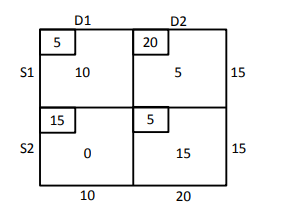
\includegraphics[width=0.75\columnwidth]{chapters/10/7/2/4/figs/fig.png}
 \end{center}
\caption{}
\label{fig:10/7/2/4Fig1}
\end{figure}
\fi

\item Find the position vector of the mid point of the vector joining the points $\vec{P}$(2, 3, 4)
and $\vec{Q}$(4, 1, –2).
\\
\solution
		\begin{enumerate}[label=\thesubsection.\arabic*,ref=\thesubsection.\theenumi]
\item Find the coordinates of the point which divides the join of $(-1,7) $ and $ (4,-3)$ in the ratio 2:3.
	\\
		\solution
	\input{chapters/10/7/2/1/section.tex}
\item Find the coordinates of the point $\vec{R}$ on the line segment joining the points $\vec{P}(-1,3)$ and $\vec{Q}(2,5)$ such that $PR=\frac{3}{5}PQ$.
\item Find the ratio in which the point $\vec{P}\brak{\frac{3}{4},\frac{5}{12}}$ divides the line segment joining the points $\vec{A}\brak{\frac{1}{2},\frac{3}{2}}$ and $ \vec{B}(2,-5)$.
\item Find the coordinates of the point which divides the line segment joining the points $(4,-3)$ and $(8,5)$ in the ratio $3:1$ internally.
\item Find the coordinates of the point $\vec{P}$ on $AD$ such that $AP : PD = 2 : 1$.
\item If the point $\vec{P} (2, 1)$ lies on the line segment joining points $\vec{A} (4, 2)$  and $ \vec{B} (8, 4)$,
then
\begin{enumerate}
	\item $AP =\frac{1}{3}{AB}$ 
\item ${AP}={PE}$
\item ${PB}=\frac{1}{3}{AB}$
\item${AP}=\frac{1}{2}{AB}$
 \end{enumerate}
\item Find the ratio in which the line segment joining the points $(-3,10)$  and  $(6,-8)$  is divided by $ (-1,6)$.
	\\
		\solution
	\input{chapters/10/7/2/4/section.tex}
\item Find the position vector of the mid point of the vector joining the points $\vec{P}$(2, 3, 4)
and $\vec{Q}$(4, 1, –2).
\\
\solution
		\input{chapters/12/10/2/16/section.tex}
\item Let $\vec{A}(4, 2), \vec{B}(6, 5)$  and $ \vec{C}(1, 4)$ be the vertices of $\triangle ABC$.
\begin{enumerate}
\item If $\vec{A}$ and  $\vec{B}$ are $(-2,-2)$ and  $(2,-4)$, respectively, find the coordinates of $\vec{P}$ such that $AP= \frac {3}{7}AB$  and $ \vec{P}$ lies on the line segment $AB$.
	\\
		\solution
	\input{chapters/10/7/2/8/section.tex}
\item Find the coordinates of the points which divide the line segment joining $A(-2,2)$  and  $\vec{B}(2,8)$ into four equal parts.
	\\
		\solution
	\input{chapters/10/7/2/9/section.tex}
\item In what ratio does the point $(-4,6)$ divide the line segment joining the points $\vec{A}(-6,0)$ and $\vec{B}(3,-8)$?
\item Given that $\vec{P}(3,2,-4), \vec{Q}(5,4,-6)$ and $\vec{R}(9,8,-10)$ are collinear. Find the ratio in which $\vec{Q}$ divides $PR$.
\item Points $\vec{A}(-6,10),\vec{B}(-4,6)$  and  $\vec{C}(3,-8)$ are collinear such that $AB=  \frac{2}{9}AC$.
\item The point which divides the line segment joining the points $\vec{P} (7, –6) $  and  $\vec{Q}(3, 4)$ in the 
ratio 1 : 2 internally lies in  which quadrant?
\item Find the coordinates of the points of trisection of the line segment joining $(4,-1)$  and  $(-2,3)$.
	\\
		\solution
	\input{chapters/10/7/2/2/section.tex}
\item Find the coordinates of the points which trisect the line segment joining the points $\vec{P}(4,2,-6)$ and $\vec{Q}(10,-16,6)$.
\item Find the coordinates of the points of trisection (i.e. points dividing to three equal parts) of the line segment joining the points $\vec{A}(2,-2)$ and $\vec{B}(-7,4)$.
\item Point $\vec{P}(5,-3)$ is one of the two points of trisection of line segment joining the points $\vec{A}(7,-2)$ and $\vec{B}(1,-5)$
\item Find the position vector of a point $\vec{R}$ which divides the line joining two points $\vec{P}$
and $\vec{Q}$ whose position vectors are $\hat{i}+2\hat{j}-\hat{k}$ and $-\hat{i}+\hat{j}+\hat{k}$ respectively, in the
ratio 2 : 1
\begin{enumerate}
    \item  internally
    \item  externally
\end{enumerate}
%\solution
%		\input{chapters/12/10/2/15/section.tex}
\item Find the coordinates of the point which divides the line segment joining the points which divides the line segment joining  the points $(-2,3,5)$ and $(1,-4,6)$ in the ratio 
\begin{enumerate}
\item $2:3$ internally,
\item $2:3$ externally
\end{enumerate}
\item Find the coordinates of the point which divides the line segment joining the points $(1,-2,3)$ and $(3,4,-5)$ in the ratio $2:3$
\begin{enumerate}
\item internally, and
\item externally
\end{enumerate}
\item Consider two points $\vec{P}$ and $\vec{Q}$ with position vectors $\overrightarrow{OP} = 3\overrightarrow{a}-2\overrightarrow{b}$ and $\overrightarrow{OQ}=\overrightarrow{a}+\overrightarrow{b}$. Find the position vector of a point $\vec{R}$ which divides the line joining $\vec{P}$ and $\vec{Q}$ in the ratio $2:1$, 
\begin{enumerate}
\item internally, and 
\item externally.
\end{enumerate}
\item The median from $\vec{A}$ meets $BC$ at $\vec{D}$. Find the coordinates of the point $\vec{D}$.
\item Find the coordinates of points $\vec{Q}$ and $\vec{R}$ on medians $BE$ and $CF$ respectively such that $BQ : QE = 2 : 1$  and  $CR : RF = 2 : 1$.
\item What do you observe?
\item If $\vec{A}, \vec{B}$ and $\vec{C}$  are the vertices of $\triangle ABC$, find the coordinates of the centroid of the triangle.
\end{enumerate}
\solution
	\input{chapters/10/7/4/7/section.tex}
\item If $\vec{P}(9a-2,-b)$ divides line segment joining $\vec{A}(3a+1,-3)$ and $\vec{B}(8a,5)$ in the ratio 3:1, find the values of $a$ and $b$.
\item Find the position vector of a point $\vec{R}$ which divides the line joining two points $\vec{P}$ and $\vec{Q}$ whose position vectors are $2\vec{a}+\vec{b}$ and $\vec{a}-3\vec{b}$ externally in the ratio $1:2$.
\item The position vector of the point which divides the join of points 2$\vec{a}$-3$\vec{b}$ $\text{and}$ $\vec{a}+\vec{b}$ in the ratio 3:1 is \rule{1cm}{0.1pt}.
\item If $\vec{a}$ and $\vec{b}$ are the postion vectors of $\vec{A}$ and $\vec{B}$, respectively, find the position vector of a point $\vec{C}$ in $BA$ produced such that $BC=1.5BA$.
\item Find the position vector of a point $\vec{R}$ which divides the line joining two points $\vec{P}$ and $\vec{Q}$ whose position vectors are $(2\vec{a}+\vec{b})$ and $(\vec{a}-3\vec{b})$
externally in the ratio 1 : 2. Also, show that $\vec{P}$ is the mid point of the line segment $RQ$.
\end{enumerate}

\item Let $\vec{A}(4, 2), \vec{B}(6, 5)$  and $ \vec{C}(1, 4)$ be the vertices of $\triangle ABC$.
\begin{enumerate}
\item If $\vec{A}$ and  $\vec{B}$ are $(-2,-2)$ and  $(2,-4)$, respectively, find the coordinates of $\vec{P}$ such that $AP= \frac {3}{7}AB$  and $ \vec{P}$ lies on the line segment $AB$.
	\\
		\solution
	\begin{enumerate}[label=\thesubsection.\arabic*,ref=\thesubsection.\theenumi]
\item Find the coordinates of the point which divides the join of $(-1,7) $ and $ (4,-3)$ in the ratio 2:3.
	\\
		\solution
	\input{chapters/10/7/2/1/section.tex}
\item Find the coordinates of the point $\vec{R}$ on the line segment joining the points $\vec{P}(-1,3)$ and $\vec{Q}(2,5)$ such that $PR=\frac{3}{5}PQ$.
\item Find the ratio in which the point $\vec{P}\brak{\frac{3}{4},\frac{5}{12}}$ divides the line segment joining the points $\vec{A}\brak{\frac{1}{2},\frac{3}{2}}$ and $ \vec{B}(2,-5)$.
\item Find the coordinates of the point which divides the line segment joining the points $(4,-3)$ and $(8,5)$ in the ratio $3:1$ internally.
\item Find the coordinates of the point $\vec{P}$ on $AD$ such that $AP : PD = 2 : 1$.
\item If the point $\vec{P} (2, 1)$ lies on the line segment joining points $\vec{A} (4, 2)$  and $ \vec{B} (8, 4)$,
then
\begin{enumerate}
	\item $AP =\frac{1}{3}{AB}$ 
\item ${AP}={PE}$
\item ${PB}=\frac{1}{3}{AB}$
\item${AP}=\frac{1}{2}{AB}$
 \end{enumerate}
\item Find the ratio in which the line segment joining the points $(-3,10)$  and  $(6,-8)$  is divided by $ (-1,6)$.
	\\
		\solution
	\input{chapters/10/7/2/4/section.tex}
\item Find the position vector of the mid point of the vector joining the points $\vec{P}$(2, 3, 4)
and $\vec{Q}$(4, 1, –2).
\\
\solution
		\input{chapters/12/10/2/16/section.tex}
\item Let $\vec{A}(4, 2), \vec{B}(6, 5)$  and $ \vec{C}(1, 4)$ be the vertices of $\triangle ABC$.
\begin{enumerate}
\item If $\vec{A}$ and  $\vec{B}$ are $(-2,-2)$ and  $(2,-4)$, respectively, find the coordinates of $\vec{P}$ such that $AP= \frac {3}{7}AB$  and $ \vec{P}$ lies on the line segment $AB$.
	\\
		\solution
	\input{chapters/10/7/2/8/section.tex}
\item Find the coordinates of the points which divide the line segment joining $A(-2,2)$  and  $\vec{B}(2,8)$ into four equal parts.
	\\
		\solution
	\input{chapters/10/7/2/9/section.tex}
\item In what ratio does the point $(-4,6)$ divide the line segment joining the points $\vec{A}(-6,0)$ and $\vec{B}(3,-8)$?
\item Given that $\vec{P}(3,2,-4), \vec{Q}(5,4,-6)$ and $\vec{R}(9,8,-10)$ are collinear. Find the ratio in which $\vec{Q}$ divides $PR$.
\item Points $\vec{A}(-6,10),\vec{B}(-4,6)$  and  $\vec{C}(3,-8)$ are collinear such that $AB=  \frac{2}{9}AC$.
\item The point which divides the line segment joining the points $\vec{P} (7, –6) $  and  $\vec{Q}(3, 4)$ in the 
ratio 1 : 2 internally lies in  which quadrant?
\item Find the coordinates of the points of trisection of the line segment joining $(4,-1)$  and  $(-2,3)$.
	\\
		\solution
	\input{chapters/10/7/2/2/section.tex}
\item Find the coordinates of the points which trisect the line segment joining the points $\vec{P}(4,2,-6)$ and $\vec{Q}(10,-16,6)$.
\item Find the coordinates of the points of trisection (i.e. points dividing to three equal parts) of the line segment joining the points $\vec{A}(2,-2)$ and $\vec{B}(-7,4)$.
\item Point $\vec{P}(5,-3)$ is one of the two points of trisection of line segment joining the points $\vec{A}(7,-2)$ and $\vec{B}(1,-5)$
\item Find the position vector of a point $\vec{R}$ which divides the line joining two points $\vec{P}$
and $\vec{Q}$ whose position vectors are $\hat{i}+2\hat{j}-\hat{k}$ and $-\hat{i}+\hat{j}+\hat{k}$ respectively, in the
ratio 2 : 1
\begin{enumerate}
    \item  internally
    \item  externally
\end{enumerate}
%\solution
%		\input{chapters/12/10/2/15/section.tex}
\item Find the coordinates of the point which divides the line segment joining the points which divides the line segment joining  the points $(-2,3,5)$ and $(1,-4,6)$ in the ratio 
\begin{enumerate}
\item $2:3$ internally,
\item $2:3$ externally
\end{enumerate}
\item Find the coordinates of the point which divides the line segment joining the points $(1,-2,3)$ and $(3,4,-5)$ in the ratio $2:3$
\begin{enumerate}
\item internally, and
\item externally
\end{enumerate}
\item Consider two points $\vec{P}$ and $\vec{Q}$ with position vectors $\overrightarrow{OP} = 3\overrightarrow{a}-2\overrightarrow{b}$ and $\overrightarrow{OQ}=\overrightarrow{a}+\overrightarrow{b}$. Find the position vector of a point $\vec{R}$ which divides the line joining $\vec{P}$ and $\vec{Q}$ in the ratio $2:1$, 
\begin{enumerate}
\item internally, and 
\item externally.
\end{enumerate}
\item The median from $\vec{A}$ meets $BC$ at $\vec{D}$. Find the coordinates of the point $\vec{D}$.
\item Find the coordinates of points $\vec{Q}$ and $\vec{R}$ on medians $BE$ and $CF$ respectively such that $BQ : QE = 2 : 1$  and  $CR : RF = 2 : 1$.
\item What do you observe?
\item If $\vec{A}, \vec{B}$ and $\vec{C}$  are the vertices of $\triangle ABC$, find the coordinates of the centroid of the triangle.
\end{enumerate}
\solution
	\input{chapters/10/7/4/7/section.tex}
\item If $\vec{P}(9a-2,-b)$ divides line segment joining $\vec{A}(3a+1,-3)$ and $\vec{B}(8a,5)$ in the ratio 3:1, find the values of $a$ and $b$.
\item Find the position vector of a point $\vec{R}$ which divides the line joining two points $\vec{P}$ and $\vec{Q}$ whose position vectors are $2\vec{a}+\vec{b}$ and $\vec{a}-3\vec{b}$ externally in the ratio $1:2$.
\item The position vector of the point which divides the join of points 2$\vec{a}$-3$\vec{b}$ $\text{and}$ $\vec{a}+\vec{b}$ in the ratio 3:1 is \rule{1cm}{0.1pt}.
\item If $\vec{a}$ and $\vec{b}$ are the postion vectors of $\vec{A}$ and $\vec{B}$, respectively, find the position vector of a point $\vec{C}$ in $BA$ produced such that $BC=1.5BA$.
\item Find the position vector of a point $\vec{R}$ which divides the line joining two points $\vec{P}$ and $\vec{Q}$ whose position vectors are $(2\vec{a}+\vec{b})$ and $(\vec{a}-3\vec{b})$
externally in the ratio 1 : 2. Also, show that $\vec{P}$ is the mid point of the line segment $RQ$.
\end{enumerate}

\item Find the coordinates of the points which divide the line segment joining $A(-2,2)$  and  $\vec{B}(2,8)$ into four equal parts.
	\\
		\solution
	\begin{enumerate}[label=\thesubsection.\arabic*,ref=\thesubsection.\theenumi]
\item Find the coordinates of the point which divides the join of $(-1,7) $ and $ (4,-3)$ in the ratio 2:3.
	\\
		\solution
	\input{chapters/10/7/2/1/section.tex}
\item Find the coordinates of the point $\vec{R}$ on the line segment joining the points $\vec{P}(-1,3)$ and $\vec{Q}(2,5)$ such that $PR=\frac{3}{5}PQ$.
\item Find the ratio in which the point $\vec{P}\brak{\frac{3}{4},\frac{5}{12}}$ divides the line segment joining the points $\vec{A}\brak{\frac{1}{2},\frac{3}{2}}$ and $ \vec{B}(2,-5)$.
\item Find the coordinates of the point which divides the line segment joining the points $(4,-3)$ and $(8,5)$ in the ratio $3:1$ internally.
\item Find the coordinates of the point $\vec{P}$ on $AD$ such that $AP : PD = 2 : 1$.
\item If the point $\vec{P} (2, 1)$ lies on the line segment joining points $\vec{A} (4, 2)$  and $ \vec{B} (8, 4)$,
then
\begin{enumerate}
	\item $AP =\frac{1}{3}{AB}$ 
\item ${AP}={PE}$
\item ${PB}=\frac{1}{3}{AB}$
\item${AP}=\frac{1}{2}{AB}$
 \end{enumerate}
\item Find the ratio in which the line segment joining the points $(-3,10)$  and  $(6,-8)$  is divided by $ (-1,6)$.
	\\
		\solution
	\input{chapters/10/7/2/4/section.tex}
\item Find the position vector of the mid point of the vector joining the points $\vec{P}$(2, 3, 4)
and $\vec{Q}$(4, 1, –2).
\\
\solution
		\input{chapters/12/10/2/16/section.tex}
\item Let $\vec{A}(4, 2), \vec{B}(6, 5)$  and $ \vec{C}(1, 4)$ be the vertices of $\triangle ABC$.
\begin{enumerate}
\item If $\vec{A}$ and  $\vec{B}$ are $(-2,-2)$ and  $(2,-4)$, respectively, find the coordinates of $\vec{P}$ such that $AP= \frac {3}{7}AB$  and $ \vec{P}$ lies on the line segment $AB$.
	\\
		\solution
	\input{chapters/10/7/2/8/section.tex}
\item Find the coordinates of the points which divide the line segment joining $A(-2,2)$  and  $\vec{B}(2,8)$ into four equal parts.
	\\
		\solution
	\input{chapters/10/7/2/9/section.tex}
\item In what ratio does the point $(-4,6)$ divide the line segment joining the points $\vec{A}(-6,0)$ and $\vec{B}(3,-8)$?
\item Given that $\vec{P}(3,2,-4), \vec{Q}(5,4,-6)$ and $\vec{R}(9,8,-10)$ are collinear. Find the ratio in which $\vec{Q}$ divides $PR$.
\item Points $\vec{A}(-6,10),\vec{B}(-4,6)$  and  $\vec{C}(3,-8)$ are collinear such that $AB=  \frac{2}{9}AC$.
\item The point which divides the line segment joining the points $\vec{P} (7, –6) $  and  $\vec{Q}(3, 4)$ in the 
ratio 1 : 2 internally lies in  which quadrant?
\item Find the coordinates of the points of trisection of the line segment joining $(4,-1)$  and  $(-2,3)$.
	\\
		\solution
	\input{chapters/10/7/2/2/section.tex}
\item Find the coordinates of the points which trisect the line segment joining the points $\vec{P}(4,2,-6)$ and $\vec{Q}(10,-16,6)$.
\item Find the coordinates of the points of trisection (i.e. points dividing to three equal parts) of the line segment joining the points $\vec{A}(2,-2)$ and $\vec{B}(-7,4)$.
\item Point $\vec{P}(5,-3)$ is one of the two points of trisection of line segment joining the points $\vec{A}(7,-2)$ and $\vec{B}(1,-5)$
\item Find the position vector of a point $\vec{R}$ which divides the line joining two points $\vec{P}$
and $\vec{Q}$ whose position vectors are $\hat{i}+2\hat{j}-\hat{k}$ and $-\hat{i}+\hat{j}+\hat{k}$ respectively, in the
ratio 2 : 1
\begin{enumerate}
    \item  internally
    \item  externally
\end{enumerate}
%\solution
%		\input{chapters/12/10/2/15/section.tex}
\item Find the coordinates of the point which divides the line segment joining the points which divides the line segment joining  the points $(-2,3,5)$ and $(1,-4,6)$ in the ratio 
\begin{enumerate}
\item $2:3$ internally,
\item $2:3$ externally
\end{enumerate}
\item Find the coordinates of the point which divides the line segment joining the points $(1,-2,3)$ and $(3,4,-5)$ in the ratio $2:3$
\begin{enumerate}
\item internally, and
\item externally
\end{enumerate}
\item Consider two points $\vec{P}$ and $\vec{Q}$ with position vectors $\overrightarrow{OP} = 3\overrightarrow{a}-2\overrightarrow{b}$ and $\overrightarrow{OQ}=\overrightarrow{a}+\overrightarrow{b}$. Find the position vector of a point $\vec{R}$ which divides the line joining $\vec{P}$ and $\vec{Q}$ in the ratio $2:1$, 
\begin{enumerate}
\item internally, and 
\item externally.
\end{enumerate}
\item The median from $\vec{A}$ meets $BC$ at $\vec{D}$. Find the coordinates of the point $\vec{D}$.
\item Find the coordinates of points $\vec{Q}$ and $\vec{R}$ on medians $BE$ and $CF$ respectively such that $BQ : QE = 2 : 1$  and  $CR : RF = 2 : 1$.
\item What do you observe?
\item If $\vec{A}, \vec{B}$ and $\vec{C}$  are the vertices of $\triangle ABC$, find the coordinates of the centroid of the triangle.
\end{enumerate}
\solution
	\input{chapters/10/7/4/7/section.tex}
\item If $\vec{P}(9a-2,-b)$ divides line segment joining $\vec{A}(3a+1,-3)$ and $\vec{B}(8a,5)$ in the ratio 3:1, find the values of $a$ and $b$.
\item Find the position vector of a point $\vec{R}$ which divides the line joining two points $\vec{P}$ and $\vec{Q}$ whose position vectors are $2\vec{a}+\vec{b}$ and $\vec{a}-3\vec{b}$ externally in the ratio $1:2$.
\item The position vector of the point which divides the join of points 2$\vec{a}$-3$\vec{b}$ $\text{and}$ $\vec{a}+\vec{b}$ in the ratio 3:1 is \rule{1cm}{0.1pt}.
\item If $\vec{a}$ and $\vec{b}$ are the postion vectors of $\vec{A}$ and $\vec{B}$, respectively, find the position vector of a point $\vec{C}$ in $BA$ produced such that $BC=1.5BA$.
\item Find the position vector of a point $\vec{R}$ which divides the line joining two points $\vec{P}$ and $\vec{Q}$ whose position vectors are $(2\vec{a}+\vec{b})$ and $(\vec{a}-3\vec{b})$
externally in the ratio 1 : 2. Also, show that $\vec{P}$ is the mid point of the line segment $RQ$.
\end{enumerate}

\item In what ratio does the point $(-4,6)$ divide the line segment joining the points $\vec{A}(-6,0)$ and $\vec{B}(3,-8)$?
\item Given that $\vec{P}(3,2,-4), \vec{Q}(5,4,-6)$ and $\vec{R}(9,8,-10)$ are collinear. Find the ratio in which $\vec{Q}$ divides $PR$.
\item Points $\vec{A}(-6,10),\vec{B}(-4,6)$  and  $\vec{C}(3,-8)$ are collinear such that $AB=  \frac{2}{9}AC$.
\item The point which divides the line segment joining the points $\vec{P} (7, –6) $  and  $\vec{Q}(3, 4)$ in the 
ratio 1 : 2 internally lies in  which quadrant?
\item Find the coordinates of the points of trisection of the line segment joining $(4,-1)$  and  $(-2,3)$.
	\\
		\solution
	Using section formula,
\begin{align}
\vec{R}=\frac{1}{1+\frac{1}{2}}\brak{\myvec{4\\-1}+\frac{1}{2}\myvec{-2\\3}}
=\myvec{2\\ \frac{1}{3}}\\
\vec{S}=\frac{1}{1+\frac{2}{1}}\brak{\myvec{4\\-1}+\frac{2}{1}\myvec{-2\\3}}
=\myvec{0\\ \frac{5}{3}}
\end{align}
which are the desired points of trisection.
\iffalse
See
		\figref{fig:chapters/10/7/2/2/Figure}
\begin{figure}[H]
\centering
\includegraphics[width=0.75\columnwidth]{chapters/10/7/2/2/figs/dj.pdf}
\caption{}
		\label{fig:chapters/10/7/2/2/Figure}
\end{figure}
\fi

\item Find the coordinates of the points which trisect the line segment joining the points $\vec{P}(4,2,-6)$ and $\vec{Q}(10,-16,6)$.
\item Find the coordinates of the points of trisection (i.e. points dividing to three equal parts) of the line segment joining the points $\vec{A}(2,-2)$ and $\vec{B}(-7,4)$.
\item Point $\vec{P}(5,-3)$ is one of the two points of trisection of line segment joining the points $\vec{A}(7,-2)$ and $\vec{B}(1,-5)$
\item Find the position vector of a point $\vec{R}$ which divides the line joining two points $\vec{P}$
and $\vec{Q}$ whose position vectors are $\hat{i}+2\hat{j}-\hat{k}$ and $-\hat{i}+\hat{j}+\hat{k}$ respectively, in the
ratio 2 : 1
\begin{enumerate}
    \item  internally
    \item  externally
\end{enumerate}
%\solution
%		\begin{enumerate}[label=\thesubsection.\arabic*,ref=\thesubsection.\theenumi]
\item Find the coordinates of the point which divides the join of $(-1,7) $ and $ (4,-3)$ in the ratio 2:3.
	\\
		\solution
	\input{chapters/10/7/2/1/section.tex}
\item Find the coordinates of the point $\vec{R}$ on the line segment joining the points $\vec{P}(-1,3)$ and $\vec{Q}(2,5)$ such that $PR=\frac{3}{5}PQ$.
\item Find the ratio in which the point $\vec{P}\brak{\frac{3}{4},\frac{5}{12}}$ divides the line segment joining the points $\vec{A}\brak{\frac{1}{2},\frac{3}{2}}$ and $ \vec{B}(2,-5)$.
\item Find the coordinates of the point which divides the line segment joining the points $(4,-3)$ and $(8,5)$ in the ratio $3:1$ internally.
\item Find the coordinates of the point $\vec{P}$ on $AD$ such that $AP : PD = 2 : 1$.
\item If the point $\vec{P} (2, 1)$ lies on the line segment joining points $\vec{A} (4, 2)$  and $ \vec{B} (8, 4)$,
then
\begin{enumerate}
	\item $AP =\frac{1}{3}{AB}$ 
\item ${AP}={PE}$
\item ${PB}=\frac{1}{3}{AB}$
\item${AP}=\frac{1}{2}{AB}$
 \end{enumerate}
\item Find the ratio in which the line segment joining the points $(-3,10)$  and  $(6,-8)$  is divided by $ (-1,6)$.
	\\
		\solution
	\input{chapters/10/7/2/4/section.tex}
\item Find the position vector of the mid point of the vector joining the points $\vec{P}$(2, 3, 4)
and $\vec{Q}$(4, 1, –2).
\\
\solution
		\input{chapters/12/10/2/16/section.tex}
\item Let $\vec{A}(4, 2), \vec{B}(6, 5)$  and $ \vec{C}(1, 4)$ be the vertices of $\triangle ABC$.
\begin{enumerate}
\item If $\vec{A}$ and  $\vec{B}$ are $(-2,-2)$ and  $(2,-4)$, respectively, find the coordinates of $\vec{P}$ such that $AP= \frac {3}{7}AB$  and $ \vec{P}$ lies on the line segment $AB$.
	\\
		\solution
	\input{chapters/10/7/2/8/section.tex}
\item Find the coordinates of the points which divide the line segment joining $A(-2,2)$  and  $\vec{B}(2,8)$ into four equal parts.
	\\
		\solution
	\input{chapters/10/7/2/9/section.tex}
\item In what ratio does the point $(-4,6)$ divide the line segment joining the points $\vec{A}(-6,0)$ and $\vec{B}(3,-8)$?
\item Given that $\vec{P}(3,2,-4), \vec{Q}(5,4,-6)$ and $\vec{R}(9,8,-10)$ are collinear. Find the ratio in which $\vec{Q}$ divides $PR$.
\item Points $\vec{A}(-6,10),\vec{B}(-4,6)$  and  $\vec{C}(3,-8)$ are collinear such that $AB=  \frac{2}{9}AC$.
\item The point which divides the line segment joining the points $\vec{P} (7, –6) $  and  $\vec{Q}(3, 4)$ in the 
ratio 1 : 2 internally lies in  which quadrant?
\item Find the coordinates of the points of trisection of the line segment joining $(4,-1)$  and  $(-2,3)$.
	\\
		\solution
	\input{chapters/10/7/2/2/section.tex}
\item Find the coordinates of the points which trisect the line segment joining the points $\vec{P}(4,2,-6)$ and $\vec{Q}(10,-16,6)$.
\item Find the coordinates of the points of trisection (i.e. points dividing to three equal parts) of the line segment joining the points $\vec{A}(2,-2)$ and $\vec{B}(-7,4)$.
\item Point $\vec{P}(5,-3)$ is one of the two points of trisection of line segment joining the points $\vec{A}(7,-2)$ and $\vec{B}(1,-5)$
\item Find the position vector of a point $\vec{R}$ which divides the line joining two points $\vec{P}$
and $\vec{Q}$ whose position vectors are $\hat{i}+2\hat{j}-\hat{k}$ and $-\hat{i}+\hat{j}+\hat{k}$ respectively, in the
ratio 2 : 1
\begin{enumerate}
    \item  internally
    \item  externally
\end{enumerate}
%\solution
%		\input{chapters/12/10/2/15/section.tex}
\item Find the coordinates of the point which divides the line segment joining the points which divides the line segment joining  the points $(-2,3,5)$ and $(1,-4,6)$ in the ratio 
\begin{enumerate}
\item $2:3$ internally,
\item $2:3$ externally
\end{enumerate}
\item Find the coordinates of the point which divides the line segment joining the points $(1,-2,3)$ and $(3,4,-5)$ in the ratio $2:3$
\begin{enumerate}
\item internally, and
\item externally
\end{enumerate}
\item Consider two points $\vec{P}$ and $\vec{Q}$ with position vectors $\overrightarrow{OP} = 3\overrightarrow{a}-2\overrightarrow{b}$ and $\overrightarrow{OQ}=\overrightarrow{a}+\overrightarrow{b}$. Find the position vector of a point $\vec{R}$ which divides the line joining $\vec{P}$ and $\vec{Q}$ in the ratio $2:1$, 
\begin{enumerate}
\item internally, and 
\item externally.
\end{enumerate}
\item The median from $\vec{A}$ meets $BC$ at $\vec{D}$. Find the coordinates of the point $\vec{D}$.
\item Find the coordinates of points $\vec{Q}$ and $\vec{R}$ on medians $BE$ and $CF$ respectively such that $BQ : QE = 2 : 1$  and  $CR : RF = 2 : 1$.
\item What do you observe?
\item If $\vec{A}, \vec{B}$ and $\vec{C}$  are the vertices of $\triangle ABC$, find the coordinates of the centroid of the triangle.
\end{enumerate}
\solution
	\input{chapters/10/7/4/7/section.tex}
\item If $\vec{P}(9a-2,-b)$ divides line segment joining $\vec{A}(3a+1,-3)$ and $\vec{B}(8a,5)$ in the ratio 3:1, find the values of $a$ and $b$.
\item Find the position vector of a point $\vec{R}$ which divides the line joining two points $\vec{P}$ and $\vec{Q}$ whose position vectors are $2\vec{a}+\vec{b}$ and $\vec{a}-3\vec{b}$ externally in the ratio $1:2$.
\item The position vector of the point which divides the join of points 2$\vec{a}$-3$\vec{b}$ $\text{and}$ $\vec{a}+\vec{b}$ in the ratio 3:1 is \rule{1cm}{0.1pt}.
\item If $\vec{a}$ and $\vec{b}$ are the postion vectors of $\vec{A}$ and $\vec{B}$, respectively, find the position vector of a point $\vec{C}$ in $BA$ produced such that $BC=1.5BA$.
\item Find the position vector of a point $\vec{R}$ which divides the line joining two points $\vec{P}$ and $\vec{Q}$ whose position vectors are $(2\vec{a}+\vec{b})$ and $(\vec{a}-3\vec{b})$
externally in the ratio 1 : 2. Also, show that $\vec{P}$ is the mid point of the line segment $RQ$.
\end{enumerate}

\item Find the coordinates of the point which divides the line segment joining the points which divides the line segment joining  the points $(-2,3,5)$ and $(1,-4,6)$ in the ratio 
\begin{enumerate}
\item $2:3$ internally,
\item $2:3$ externally
\end{enumerate}
\item Find the coordinates of the point which divides the line segment joining the points $(1,-2,3)$ and $(3,4,-5)$ in the ratio $2:3$
\begin{enumerate}
\item internally, and
\item externally
\end{enumerate}
\item Consider two points $\vec{P}$ and $\vec{Q}$ with position vectors $\overrightarrow{OP} = 3\overrightarrow{a}-2\overrightarrow{b}$ and $\overrightarrow{OQ}=\overrightarrow{a}+\overrightarrow{b}$. Find the position vector of a point $\vec{R}$ which divides the line joining $\vec{P}$ and $\vec{Q}$ in the ratio $2:1$, 
\begin{enumerate}
\item internally, and 
\item externally.
\end{enumerate}
\item The median from $\vec{A}$ meets $BC$ at $\vec{D}$. Find the coordinates of the point $\vec{D}$.
\item Find the coordinates of points $\vec{Q}$ and $\vec{R}$ on medians $BE$ and $CF$ respectively such that $BQ : QE = 2 : 1$  and  $CR : RF = 2 : 1$.
\item What do you observe?
\item If $\vec{A}, \vec{B}$ and $\vec{C}$  are the vertices of $\triangle ABC$, find the coordinates of the centroid of the triangle.
\end{enumerate}
\solution
	\begin{enumerate}[label=\thesubsection.\arabic*,ref=\thesubsection.\theenumi]
\item Find the coordinates of the point which divides the join of $(-1,7) $ and $ (4,-3)$ in the ratio 2:3.
	\\
		\solution
	\input{chapters/10/7/2/1/section.tex}
\item Find the coordinates of the point $\vec{R}$ on the line segment joining the points $\vec{P}(-1,3)$ and $\vec{Q}(2,5)$ such that $PR=\frac{3}{5}PQ$.
\item Find the ratio in which the point $\vec{P}\brak{\frac{3}{4},\frac{5}{12}}$ divides the line segment joining the points $\vec{A}\brak{\frac{1}{2},\frac{3}{2}}$ and $ \vec{B}(2,-5)$.
\item Find the coordinates of the point which divides the line segment joining the points $(4,-3)$ and $(8,5)$ in the ratio $3:1$ internally.
\item Find the coordinates of the point $\vec{P}$ on $AD$ such that $AP : PD = 2 : 1$.
\item If the point $\vec{P} (2, 1)$ lies on the line segment joining points $\vec{A} (4, 2)$  and $ \vec{B} (8, 4)$,
then
\begin{enumerate}
	\item $AP =\frac{1}{3}{AB}$ 
\item ${AP}={PE}$
\item ${PB}=\frac{1}{3}{AB}$
\item${AP}=\frac{1}{2}{AB}$
 \end{enumerate}
\item Find the ratio in which the line segment joining the points $(-3,10)$  and  $(6,-8)$  is divided by $ (-1,6)$.
	\\
		\solution
	\input{chapters/10/7/2/4/section.tex}
\item Find the position vector of the mid point of the vector joining the points $\vec{P}$(2, 3, 4)
and $\vec{Q}$(4, 1, –2).
\\
\solution
		\input{chapters/12/10/2/16/section.tex}
\item Let $\vec{A}(4, 2), \vec{B}(6, 5)$  and $ \vec{C}(1, 4)$ be the vertices of $\triangle ABC$.
\begin{enumerate}
\item If $\vec{A}$ and  $\vec{B}$ are $(-2,-2)$ and  $(2,-4)$, respectively, find the coordinates of $\vec{P}$ such that $AP= \frac {3}{7}AB$  and $ \vec{P}$ lies on the line segment $AB$.
	\\
		\solution
	\input{chapters/10/7/2/8/section.tex}
\item Find the coordinates of the points which divide the line segment joining $A(-2,2)$  and  $\vec{B}(2,8)$ into four equal parts.
	\\
		\solution
	\input{chapters/10/7/2/9/section.tex}
\item In what ratio does the point $(-4,6)$ divide the line segment joining the points $\vec{A}(-6,0)$ and $\vec{B}(3,-8)$?
\item Given that $\vec{P}(3,2,-4), \vec{Q}(5,4,-6)$ and $\vec{R}(9,8,-10)$ are collinear. Find the ratio in which $\vec{Q}$ divides $PR$.
\item Points $\vec{A}(-6,10),\vec{B}(-4,6)$  and  $\vec{C}(3,-8)$ are collinear such that $AB=  \frac{2}{9}AC$.
\item The point which divides the line segment joining the points $\vec{P} (7, –6) $  and  $\vec{Q}(3, 4)$ in the 
ratio 1 : 2 internally lies in  which quadrant?
\item Find the coordinates of the points of trisection of the line segment joining $(4,-1)$  and  $(-2,3)$.
	\\
		\solution
	\input{chapters/10/7/2/2/section.tex}
\item Find the coordinates of the points which trisect the line segment joining the points $\vec{P}(4,2,-6)$ and $\vec{Q}(10,-16,6)$.
\item Find the coordinates of the points of trisection (i.e. points dividing to three equal parts) of the line segment joining the points $\vec{A}(2,-2)$ and $\vec{B}(-7,4)$.
\item Point $\vec{P}(5,-3)$ is one of the two points of trisection of line segment joining the points $\vec{A}(7,-2)$ and $\vec{B}(1,-5)$
\item Find the position vector of a point $\vec{R}$ which divides the line joining two points $\vec{P}$
and $\vec{Q}$ whose position vectors are $\hat{i}+2\hat{j}-\hat{k}$ and $-\hat{i}+\hat{j}+\hat{k}$ respectively, in the
ratio 2 : 1
\begin{enumerate}
    \item  internally
    \item  externally
\end{enumerate}
%\solution
%		\input{chapters/12/10/2/15/section.tex}
\item Find the coordinates of the point which divides the line segment joining the points which divides the line segment joining  the points $(-2,3,5)$ and $(1,-4,6)$ in the ratio 
\begin{enumerate}
\item $2:3$ internally,
\item $2:3$ externally
\end{enumerate}
\item Find the coordinates of the point which divides the line segment joining the points $(1,-2,3)$ and $(3,4,-5)$ in the ratio $2:3$
\begin{enumerate}
\item internally, and
\item externally
\end{enumerate}
\item Consider two points $\vec{P}$ and $\vec{Q}$ with position vectors $\overrightarrow{OP} = 3\overrightarrow{a}-2\overrightarrow{b}$ and $\overrightarrow{OQ}=\overrightarrow{a}+\overrightarrow{b}$. Find the position vector of a point $\vec{R}$ which divides the line joining $\vec{P}$ and $\vec{Q}$ in the ratio $2:1$, 
\begin{enumerate}
\item internally, and 
\item externally.
\end{enumerate}
\item The median from $\vec{A}$ meets $BC$ at $\vec{D}$. Find the coordinates of the point $\vec{D}$.
\item Find the coordinates of points $\vec{Q}$ and $\vec{R}$ on medians $BE$ and $CF$ respectively such that $BQ : QE = 2 : 1$  and  $CR : RF = 2 : 1$.
\item What do you observe?
\item If $\vec{A}, \vec{B}$ and $\vec{C}$  are the vertices of $\triangle ABC$, find the coordinates of the centroid of the triangle.
\end{enumerate}
\solution
	\input{chapters/10/7/4/7/section.tex}
\item If $\vec{P}(9a-2,-b)$ divides line segment joining $\vec{A}(3a+1,-3)$ and $\vec{B}(8a,5)$ in the ratio 3:1, find the values of $a$ and $b$.
\item Find the position vector of a point $\vec{R}$ which divides the line joining two points $\vec{P}$ and $\vec{Q}$ whose position vectors are $2\vec{a}+\vec{b}$ and $\vec{a}-3\vec{b}$ externally in the ratio $1:2$.
\item The position vector of the point which divides the join of points 2$\vec{a}$-3$\vec{b}$ $\text{and}$ $\vec{a}+\vec{b}$ in the ratio 3:1 is \rule{1cm}{0.1pt}.
\item If $\vec{a}$ and $\vec{b}$ are the postion vectors of $\vec{A}$ and $\vec{B}$, respectively, find the position vector of a point $\vec{C}$ in $BA$ produced such that $BC=1.5BA$.
\item Find the position vector of a point $\vec{R}$ which divides the line joining two points $\vec{P}$ and $\vec{Q}$ whose position vectors are $(2\vec{a}+\vec{b})$ and $(\vec{a}-3\vec{b})$
externally in the ratio 1 : 2. Also, show that $\vec{P}$ is the mid point of the line segment $RQ$.
\end{enumerate}

\item If $\vec{P}(9a-2,-b)$ divides line segment joining $\vec{A}(3a+1,-3)$ and $\vec{B}(8a,5)$ in the ratio 3:1, find the values of $a$ and $b$.
\item Find the position vector of a point $\vec{R}$ which divides the line joining two points $\vec{P}$ and $\vec{Q}$ whose position vectors are $2\vec{a}+\vec{b}$ and $\vec{a}-3\vec{b}$ externally in the ratio $1:2$.
\item The position vector of the point which divides the join of points 2$\vec{a}$-3$\vec{b}$ $\text{and}$ $\vec{a}+\vec{b}$ in the ratio 3:1 is \rule{1cm}{0.1pt}.
\item If $\vec{a}$ and $\vec{b}$ are the postion vectors of $\vec{A}$ and $\vec{B}$, respectively, find the position vector of a point $\vec{C}$ in $BA$ produced such that $BC=1.5BA$.
\item Find the position vector of a point $\vec{R}$ which divides the line joining two points $\vec{P}$ and $\vec{Q}$ whose position vectors are $(2\vec{a}+\vec{b})$ and $(\vec{a}-3\vec{b})$
externally in the ratio 1 : 2. Also, show that $\vec{P}$ is the mid point of the line segment $RQ$.
\end{enumerate}

\item Find the coordinates of the points which divide the line segment joining $A(-2,2)$  and  $\vec{B}(2,8)$ into four equal parts.
	\\
		\solution
	\begin{enumerate}[label=\thesubsection.\arabic*,ref=\thesubsection.\theenumi]
\item Find the coordinates of the point which divides the join of $(-1,7) $ and $ (4,-3)$ in the ratio 2:3.
	\\
		\solution
	\begin{enumerate}[label=\thesubsection.\arabic*,ref=\thesubsection.\theenumi]
\item Find the coordinates of the point which divides the join of $(-1,7) $ and $ (4,-3)$ in the ratio 2:3.
	\\
		\solution
	\input{chapters/10/7/2/1/section.tex}
\item Find the coordinates of the point $\vec{R}$ on the line segment joining the points $\vec{P}(-1,3)$ and $\vec{Q}(2,5)$ such that $PR=\frac{3}{5}PQ$.
\item Find the ratio in which the point $\vec{P}\brak{\frac{3}{4},\frac{5}{12}}$ divides the line segment joining the points $\vec{A}\brak{\frac{1}{2},\frac{3}{2}}$ and $ \vec{B}(2,-5)$.
\item Find the coordinates of the point which divides the line segment joining the points $(4,-3)$ and $(8,5)$ in the ratio $3:1$ internally.
\item Find the coordinates of the point $\vec{P}$ on $AD$ such that $AP : PD = 2 : 1$.
\item If the point $\vec{P} (2, 1)$ lies on the line segment joining points $\vec{A} (4, 2)$  and $ \vec{B} (8, 4)$,
then
\begin{enumerate}
	\item $AP =\frac{1}{3}{AB}$ 
\item ${AP}={PE}$
\item ${PB}=\frac{1}{3}{AB}$
\item${AP}=\frac{1}{2}{AB}$
 \end{enumerate}
\item Find the ratio in which the line segment joining the points $(-3,10)$  and  $(6,-8)$  is divided by $ (-1,6)$.
	\\
		\solution
	\input{chapters/10/7/2/4/section.tex}
\item Find the position vector of the mid point of the vector joining the points $\vec{P}$(2, 3, 4)
and $\vec{Q}$(4, 1, –2).
\\
\solution
		\input{chapters/12/10/2/16/section.tex}
\item Let $\vec{A}(4, 2), \vec{B}(6, 5)$  and $ \vec{C}(1, 4)$ be the vertices of $\triangle ABC$.
\begin{enumerate}
\item If $\vec{A}$ and  $\vec{B}$ are $(-2,-2)$ and  $(2,-4)$, respectively, find the coordinates of $\vec{P}$ such that $AP= \frac {3}{7}AB$  and $ \vec{P}$ lies on the line segment $AB$.
	\\
		\solution
	\input{chapters/10/7/2/8/section.tex}
\item Find the coordinates of the points which divide the line segment joining $A(-2,2)$  and  $\vec{B}(2,8)$ into four equal parts.
	\\
		\solution
	\input{chapters/10/7/2/9/section.tex}
\item In what ratio does the point $(-4,6)$ divide the line segment joining the points $\vec{A}(-6,0)$ and $\vec{B}(3,-8)$?
\item Given that $\vec{P}(3,2,-4), \vec{Q}(5,4,-6)$ and $\vec{R}(9,8,-10)$ are collinear. Find the ratio in which $\vec{Q}$ divides $PR$.
\item Points $\vec{A}(-6,10),\vec{B}(-4,6)$  and  $\vec{C}(3,-8)$ are collinear such that $AB=  \frac{2}{9}AC$.
\item The point which divides the line segment joining the points $\vec{P} (7, –6) $  and  $\vec{Q}(3, 4)$ in the 
ratio 1 : 2 internally lies in  which quadrant?
\item Find the coordinates of the points of trisection of the line segment joining $(4,-1)$  and  $(-2,3)$.
	\\
		\solution
	\input{chapters/10/7/2/2/section.tex}
\item Find the coordinates of the points which trisect the line segment joining the points $\vec{P}(4,2,-6)$ and $\vec{Q}(10,-16,6)$.
\item Find the coordinates of the points of trisection (i.e. points dividing to three equal parts) of the line segment joining the points $\vec{A}(2,-2)$ and $\vec{B}(-7,4)$.
\item Point $\vec{P}(5,-3)$ is one of the two points of trisection of line segment joining the points $\vec{A}(7,-2)$ and $\vec{B}(1,-5)$
\item Find the position vector of a point $\vec{R}$ which divides the line joining two points $\vec{P}$
and $\vec{Q}$ whose position vectors are $\hat{i}+2\hat{j}-\hat{k}$ and $-\hat{i}+\hat{j}+\hat{k}$ respectively, in the
ratio 2 : 1
\begin{enumerate}
    \item  internally
    \item  externally
\end{enumerate}
%\solution
%		\input{chapters/12/10/2/15/section.tex}
\item Find the coordinates of the point which divides the line segment joining the points which divides the line segment joining  the points $(-2,3,5)$ and $(1,-4,6)$ in the ratio 
\begin{enumerate}
\item $2:3$ internally,
\item $2:3$ externally
\end{enumerate}
\item Find the coordinates of the point which divides the line segment joining the points $(1,-2,3)$ and $(3,4,-5)$ in the ratio $2:3$
\begin{enumerate}
\item internally, and
\item externally
\end{enumerate}
\item Consider two points $\vec{P}$ and $\vec{Q}$ with position vectors $\overrightarrow{OP} = 3\overrightarrow{a}-2\overrightarrow{b}$ and $\overrightarrow{OQ}=\overrightarrow{a}+\overrightarrow{b}$. Find the position vector of a point $\vec{R}$ which divides the line joining $\vec{P}$ and $\vec{Q}$ in the ratio $2:1$, 
\begin{enumerate}
\item internally, and 
\item externally.
\end{enumerate}
\item The median from $\vec{A}$ meets $BC$ at $\vec{D}$. Find the coordinates of the point $\vec{D}$.
\item Find the coordinates of points $\vec{Q}$ and $\vec{R}$ on medians $BE$ and $CF$ respectively such that $BQ : QE = 2 : 1$  and  $CR : RF = 2 : 1$.
\item What do you observe?
\item If $\vec{A}, \vec{B}$ and $\vec{C}$  are the vertices of $\triangle ABC$, find the coordinates of the centroid of the triangle.
\end{enumerate}
\solution
	\input{chapters/10/7/4/7/section.tex}
\item If $\vec{P}(9a-2,-b)$ divides line segment joining $\vec{A}(3a+1,-3)$ and $\vec{B}(8a,5)$ in the ratio 3:1, find the values of $a$ and $b$.
\item Find the position vector of a point $\vec{R}$ which divides the line joining two points $\vec{P}$ and $\vec{Q}$ whose position vectors are $2\vec{a}+\vec{b}$ and $\vec{a}-3\vec{b}$ externally in the ratio $1:2$.
\item The position vector of the point which divides the join of points 2$\vec{a}$-3$\vec{b}$ $\text{and}$ $\vec{a}+\vec{b}$ in the ratio 3:1 is \rule{1cm}{0.1pt}.
\item If $\vec{a}$ and $\vec{b}$ are the postion vectors of $\vec{A}$ and $\vec{B}$, respectively, find the position vector of a point $\vec{C}$ in $BA$ produced such that $BC=1.5BA$.
\item Find the position vector of a point $\vec{R}$ which divides the line joining two points $\vec{P}$ and $\vec{Q}$ whose position vectors are $(2\vec{a}+\vec{b})$ and $(\vec{a}-3\vec{b})$
externally in the ratio 1 : 2. Also, show that $\vec{P}$ is the mid point of the line segment $RQ$.
\end{enumerate}

\item Find the coordinates of the point $\vec{R}$ on the line segment joining the points $\vec{P}(-1,3)$ and $\vec{Q}(2,5)$ such that $PR=\frac{3}{5}PQ$.
\item Find the ratio in which the point $\vec{P}\brak{\frac{3}{4},\frac{5}{12}}$ divides the line segment joining the points $\vec{A}\brak{\frac{1}{2},\frac{3}{2}}$ and $ \vec{B}(2,-5)$.
\item Find the coordinates of the point which divides the line segment joining the points $(4,-3)$ and $(8,5)$ in the ratio $3:1$ internally.
\item Find the coordinates of the point $\vec{P}$ on $AD$ such that $AP : PD = 2 : 1$.
\item If the point $\vec{P} (2, 1)$ lies on the line segment joining points $\vec{A} (4, 2)$  and $ \vec{B} (8, 4)$,
then
\begin{enumerate}
	\item $AP =\frac{1}{3}{AB}$ 
\item ${AP}={PE}$
\item ${PB}=\frac{1}{3}{AB}$
\item${AP}=\frac{1}{2}{AB}$
 \end{enumerate}
\item Find the ratio in which the line segment joining the points $(-3,10)$  and  $(6,-8)$  is divided by $ (-1,6)$.
	\\
		\solution
	\iffalse
Using section formula,
\begin{align}
         \myvec{-1\\6} &=\frac{{\myvec{-3\\10}+k\myvec{6\\-8}}}{1+k}\\
	 \implies 7k\myvec{1 \\ -2} &= 2\myvec{1 \\ -2}
	 \\
	 \text{or, } k &= \frac{2}{7}.
\end{align}
\fi
In 
			\eqref{eq:section_formula-k}, substituting
			\begin{align}
				\vec{B} &= \myvec{-3\\10}, \vec{C} = \myvec{6\\-8}, \vec{D} = \myvec{-1\\6},
				\\
				k &= \frac{\myvec{-2 & 4}\myvec{-7 \\ 14}}{\norm{\myvec{-7 \\ 14}}^2} = \frac{2}{7}
			\end{align}
\iffalse
See \figref{fig:10/7/2/4Fig1}.
\begin{figure}[H]
 \begin{center}
  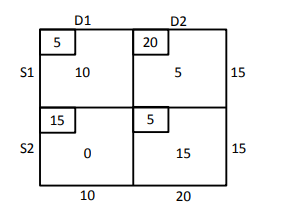
\includegraphics[width=0.75\columnwidth]{chapters/10/7/2/4/figs/fig.png}
 \end{center}
\caption{}
\label{fig:10/7/2/4Fig1}
\end{figure}
\fi

\item Find the position vector of the mid point of the vector joining the points $\vec{P}$(2, 3, 4)
and $\vec{Q}$(4, 1, –2).
\\
\solution
		\begin{enumerate}[label=\thesubsection.\arabic*,ref=\thesubsection.\theenumi]
\item Find the coordinates of the point which divides the join of $(-1,7) $ and $ (4,-3)$ in the ratio 2:3.
	\\
		\solution
	\input{chapters/10/7/2/1/section.tex}
\item Find the coordinates of the point $\vec{R}$ on the line segment joining the points $\vec{P}(-1,3)$ and $\vec{Q}(2,5)$ such that $PR=\frac{3}{5}PQ$.
\item Find the ratio in which the point $\vec{P}\brak{\frac{3}{4},\frac{5}{12}}$ divides the line segment joining the points $\vec{A}\brak{\frac{1}{2},\frac{3}{2}}$ and $ \vec{B}(2,-5)$.
\item Find the coordinates of the point which divides the line segment joining the points $(4,-3)$ and $(8,5)$ in the ratio $3:1$ internally.
\item Find the coordinates of the point $\vec{P}$ on $AD$ such that $AP : PD = 2 : 1$.
\item If the point $\vec{P} (2, 1)$ lies on the line segment joining points $\vec{A} (4, 2)$  and $ \vec{B} (8, 4)$,
then
\begin{enumerate}
	\item $AP =\frac{1}{3}{AB}$ 
\item ${AP}={PE}$
\item ${PB}=\frac{1}{3}{AB}$
\item${AP}=\frac{1}{2}{AB}$
 \end{enumerate}
\item Find the ratio in which the line segment joining the points $(-3,10)$  and  $(6,-8)$  is divided by $ (-1,6)$.
	\\
		\solution
	\input{chapters/10/7/2/4/section.tex}
\item Find the position vector of the mid point of the vector joining the points $\vec{P}$(2, 3, 4)
and $\vec{Q}$(4, 1, –2).
\\
\solution
		\input{chapters/12/10/2/16/section.tex}
\item Let $\vec{A}(4, 2), \vec{B}(6, 5)$  and $ \vec{C}(1, 4)$ be the vertices of $\triangle ABC$.
\begin{enumerate}
\item If $\vec{A}$ and  $\vec{B}$ are $(-2,-2)$ and  $(2,-4)$, respectively, find the coordinates of $\vec{P}$ such that $AP= \frac {3}{7}AB$  and $ \vec{P}$ lies on the line segment $AB$.
	\\
		\solution
	\input{chapters/10/7/2/8/section.tex}
\item Find the coordinates of the points which divide the line segment joining $A(-2,2)$  and  $\vec{B}(2,8)$ into four equal parts.
	\\
		\solution
	\input{chapters/10/7/2/9/section.tex}
\item In what ratio does the point $(-4,6)$ divide the line segment joining the points $\vec{A}(-6,0)$ and $\vec{B}(3,-8)$?
\item Given that $\vec{P}(3,2,-4), \vec{Q}(5,4,-6)$ and $\vec{R}(9,8,-10)$ are collinear. Find the ratio in which $\vec{Q}$ divides $PR$.
\item Points $\vec{A}(-6,10),\vec{B}(-4,6)$  and  $\vec{C}(3,-8)$ are collinear such that $AB=  \frac{2}{9}AC$.
\item The point which divides the line segment joining the points $\vec{P} (7, –6) $  and  $\vec{Q}(3, 4)$ in the 
ratio 1 : 2 internally lies in  which quadrant?
\item Find the coordinates of the points of trisection of the line segment joining $(4,-1)$  and  $(-2,3)$.
	\\
		\solution
	\input{chapters/10/7/2/2/section.tex}
\item Find the coordinates of the points which trisect the line segment joining the points $\vec{P}(4,2,-6)$ and $\vec{Q}(10,-16,6)$.
\item Find the coordinates of the points of trisection (i.e. points dividing to three equal parts) of the line segment joining the points $\vec{A}(2,-2)$ and $\vec{B}(-7,4)$.
\item Point $\vec{P}(5,-3)$ is one of the two points of trisection of line segment joining the points $\vec{A}(7,-2)$ and $\vec{B}(1,-5)$
\item Find the position vector of a point $\vec{R}$ which divides the line joining two points $\vec{P}$
and $\vec{Q}$ whose position vectors are $\hat{i}+2\hat{j}-\hat{k}$ and $-\hat{i}+\hat{j}+\hat{k}$ respectively, in the
ratio 2 : 1
\begin{enumerate}
    \item  internally
    \item  externally
\end{enumerate}
%\solution
%		\input{chapters/12/10/2/15/section.tex}
\item Find the coordinates of the point which divides the line segment joining the points which divides the line segment joining  the points $(-2,3,5)$ and $(1,-4,6)$ in the ratio 
\begin{enumerate}
\item $2:3$ internally,
\item $2:3$ externally
\end{enumerate}
\item Find the coordinates of the point which divides the line segment joining the points $(1,-2,3)$ and $(3,4,-5)$ in the ratio $2:3$
\begin{enumerate}
\item internally, and
\item externally
\end{enumerate}
\item Consider two points $\vec{P}$ and $\vec{Q}$ with position vectors $\overrightarrow{OP} = 3\overrightarrow{a}-2\overrightarrow{b}$ and $\overrightarrow{OQ}=\overrightarrow{a}+\overrightarrow{b}$. Find the position vector of a point $\vec{R}$ which divides the line joining $\vec{P}$ and $\vec{Q}$ in the ratio $2:1$, 
\begin{enumerate}
\item internally, and 
\item externally.
\end{enumerate}
\item The median from $\vec{A}$ meets $BC$ at $\vec{D}$. Find the coordinates of the point $\vec{D}$.
\item Find the coordinates of points $\vec{Q}$ and $\vec{R}$ on medians $BE$ and $CF$ respectively such that $BQ : QE = 2 : 1$  and  $CR : RF = 2 : 1$.
\item What do you observe?
\item If $\vec{A}, \vec{B}$ and $\vec{C}$  are the vertices of $\triangle ABC$, find the coordinates of the centroid of the triangle.
\end{enumerate}
\solution
	\input{chapters/10/7/4/7/section.tex}
\item If $\vec{P}(9a-2,-b)$ divides line segment joining $\vec{A}(3a+1,-3)$ and $\vec{B}(8a,5)$ in the ratio 3:1, find the values of $a$ and $b$.
\item Find the position vector of a point $\vec{R}$ which divides the line joining two points $\vec{P}$ and $\vec{Q}$ whose position vectors are $2\vec{a}+\vec{b}$ and $\vec{a}-3\vec{b}$ externally in the ratio $1:2$.
\item The position vector of the point which divides the join of points 2$\vec{a}$-3$\vec{b}$ $\text{and}$ $\vec{a}+\vec{b}$ in the ratio 3:1 is \rule{1cm}{0.1pt}.
\item If $\vec{a}$ and $\vec{b}$ are the postion vectors of $\vec{A}$ and $\vec{B}$, respectively, find the position vector of a point $\vec{C}$ in $BA$ produced such that $BC=1.5BA$.
\item Find the position vector of a point $\vec{R}$ which divides the line joining two points $\vec{P}$ and $\vec{Q}$ whose position vectors are $(2\vec{a}+\vec{b})$ and $(\vec{a}-3\vec{b})$
externally in the ratio 1 : 2. Also, show that $\vec{P}$ is the mid point of the line segment $RQ$.
\end{enumerate}

\item Let $\vec{A}(4, 2), \vec{B}(6, 5)$  and $ \vec{C}(1, 4)$ be the vertices of $\triangle ABC$.
\begin{enumerate}
\item If $\vec{A}$ and  $\vec{B}$ are $(-2,-2)$ and  $(2,-4)$, respectively, find the coordinates of $\vec{P}$ such that $AP= \frac {3}{7}AB$  and $ \vec{P}$ lies on the line segment $AB$.
	\\
		\solution
	\begin{enumerate}[label=\thesubsection.\arabic*,ref=\thesubsection.\theenumi]
\item Find the coordinates of the point which divides the join of $(-1,7) $ and $ (4,-3)$ in the ratio 2:3.
	\\
		\solution
	\input{chapters/10/7/2/1/section.tex}
\item Find the coordinates of the point $\vec{R}$ on the line segment joining the points $\vec{P}(-1,3)$ and $\vec{Q}(2,5)$ such that $PR=\frac{3}{5}PQ$.
\item Find the ratio in which the point $\vec{P}\brak{\frac{3}{4},\frac{5}{12}}$ divides the line segment joining the points $\vec{A}\brak{\frac{1}{2},\frac{3}{2}}$ and $ \vec{B}(2,-5)$.
\item Find the coordinates of the point which divides the line segment joining the points $(4,-3)$ and $(8,5)$ in the ratio $3:1$ internally.
\item Find the coordinates of the point $\vec{P}$ on $AD$ such that $AP : PD = 2 : 1$.
\item If the point $\vec{P} (2, 1)$ lies on the line segment joining points $\vec{A} (4, 2)$  and $ \vec{B} (8, 4)$,
then
\begin{enumerate}
	\item $AP =\frac{1}{3}{AB}$ 
\item ${AP}={PE}$
\item ${PB}=\frac{1}{3}{AB}$
\item${AP}=\frac{1}{2}{AB}$
 \end{enumerate}
\item Find the ratio in which the line segment joining the points $(-3,10)$  and  $(6,-8)$  is divided by $ (-1,6)$.
	\\
		\solution
	\input{chapters/10/7/2/4/section.tex}
\item Find the position vector of the mid point of the vector joining the points $\vec{P}$(2, 3, 4)
and $\vec{Q}$(4, 1, –2).
\\
\solution
		\input{chapters/12/10/2/16/section.tex}
\item Let $\vec{A}(4, 2), \vec{B}(6, 5)$  and $ \vec{C}(1, 4)$ be the vertices of $\triangle ABC$.
\begin{enumerate}
\item If $\vec{A}$ and  $\vec{B}$ are $(-2,-2)$ and  $(2,-4)$, respectively, find the coordinates of $\vec{P}$ such that $AP= \frac {3}{7}AB$  and $ \vec{P}$ lies on the line segment $AB$.
	\\
		\solution
	\input{chapters/10/7/2/8/section.tex}
\item Find the coordinates of the points which divide the line segment joining $A(-2,2)$  and  $\vec{B}(2,8)$ into four equal parts.
	\\
		\solution
	\input{chapters/10/7/2/9/section.tex}
\item In what ratio does the point $(-4,6)$ divide the line segment joining the points $\vec{A}(-6,0)$ and $\vec{B}(3,-8)$?
\item Given that $\vec{P}(3,2,-4), \vec{Q}(5,4,-6)$ and $\vec{R}(9,8,-10)$ are collinear. Find the ratio in which $\vec{Q}$ divides $PR$.
\item Points $\vec{A}(-6,10),\vec{B}(-4,6)$  and  $\vec{C}(3,-8)$ are collinear such that $AB=  \frac{2}{9}AC$.
\item The point which divides the line segment joining the points $\vec{P} (7, –6) $  and  $\vec{Q}(3, 4)$ in the 
ratio 1 : 2 internally lies in  which quadrant?
\item Find the coordinates of the points of trisection of the line segment joining $(4,-1)$  and  $(-2,3)$.
	\\
		\solution
	\input{chapters/10/7/2/2/section.tex}
\item Find the coordinates of the points which trisect the line segment joining the points $\vec{P}(4,2,-6)$ and $\vec{Q}(10,-16,6)$.
\item Find the coordinates of the points of trisection (i.e. points dividing to three equal parts) of the line segment joining the points $\vec{A}(2,-2)$ and $\vec{B}(-7,4)$.
\item Point $\vec{P}(5,-3)$ is one of the two points of trisection of line segment joining the points $\vec{A}(7,-2)$ and $\vec{B}(1,-5)$
\item Find the position vector of a point $\vec{R}$ which divides the line joining two points $\vec{P}$
and $\vec{Q}$ whose position vectors are $\hat{i}+2\hat{j}-\hat{k}$ and $-\hat{i}+\hat{j}+\hat{k}$ respectively, in the
ratio 2 : 1
\begin{enumerate}
    \item  internally
    \item  externally
\end{enumerate}
%\solution
%		\input{chapters/12/10/2/15/section.tex}
\item Find the coordinates of the point which divides the line segment joining the points which divides the line segment joining  the points $(-2,3,5)$ and $(1,-4,6)$ in the ratio 
\begin{enumerate}
\item $2:3$ internally,
\item $2:3$ externally
\end{enumerate}
\item Find the coordinates of the point which divides the line segment joining the points $(1,-2,3)$ and $(3,4,-5)$ in the ratio $2:3$
\begin{enumerate}
\item internally, and
\item externally
\end{enumerate}
\item Consider two points $\vec{P}$ and $\vec{Q}$ with position vectors $\overrightarrow{OP} = 3\overrightarrow{a}-2\overrightarrow{b}$ and $\overrightarrow{OQ}=\overrightarrow{a}+\overrightarrow{b}$. Find the position vector of a point $\vec{R}$ which divides the line joining $\vec{P}$ and $\vec{Q}$ in the ratio $2:1$, 
\begin{enumerate}
\item internally, and 
\item externally.
\end{enumerate}
\item The median from $\vec{A}$ meets $BC$ at $\vec{D}$. Find the coordinates of the point $\vec{D}$.
\item Find the coordinates of points $\vec{Q}$ and $\vec{R}$ on medians $BE$ and $CF$ respectively such that $BQ : QE = 2 : 1$  and  $CR : RF = 2 : 1$.
\item What do you observe?
\item If $\vec{A}, \vec{B}$ and $\vec{C}$  are the vertices of $\triangle ABC$, find the coordinates of the centroid of the triangle.
\end{enumerate}
\solution
	\input{chapters/10/7/4/7/section.tex}
\item If $\vec{P}(9a-2,-b)$ divides line segment joining $\vec{A}(3a+1,-3)$ and $\vec{B}(8a,5)$ in the ratio 3:1, find the values of $a$ and $b$.
\item Find the position vector of a point $\vec{R}$ which divides the line joining two points $\vec{P}$ and $\vec{Q}$ whose position vectors are $2\vec{a}+\vec{b}$ and $\vec{a}-3\vec{b}$ externally in the ratio $1:2$.
\item The position vector of the point which divides the join of points 2$\vec{a}$-3$\vec{b}$ $\text{and}$ $\vec{a}+\vec{b}$ in the ratio 3:1 is \rule{1cm}{0.1pt}.
\item If $\vec{a}$ and $\vec{b}$ are the postion vectors of $\vec{A}$ and $\vec{B}$, respectively, find the position vector of a point $\vec{C}$ in $BA$ produced such that $BC=1.5BA$.
\item Find the position vector of a point $\vec{R}$ which divides the line joining two points $\vec{P}$ and $\vec{Q}$ whose position vectors are $(2\vec{a}+\vec{b})$ and $(\vec{a}-3\vec{b})$
externally in the ratio 1 : 2. Also, show that $\vec{P}$ is the mid point of the line segment $RQ$.
\end{enumerate}

\item Find the coordinates of the points which divide the line segment joining $A(-2,2)$  and  $\vec{B}(2,8)$ into four equal parts.
	\\
		\solution
	\begin{enumerate}[label=\thesubsection.\arabic*,ref=\thesubsection.\theenumi]
\item Find the coordinates of the point which divides the join of $(-1,7) $ and $ (4,-3)$ in the ratio 2:3.
	\\
		\solution
	\input{chapters/10/7/2/1/section.tex}
\item Find the coordinates of the point $\vec{R}$ on the line segment joining the points $\vec{P}(-1,3)$ and $\vec{Q}(2,5)$ such that $PR=\frac{3}{5}PQ$.
\item Find the ratio in which the point $\vec{P}\brak{\frac{3}{4},\frac{5}{12}}$ divides the line segment joining the points $\vec{A}\brak{\frac{1}{2},\frac{3}{2}}$ and $ \vec{B}(2,-5)$.
\item Find the coordinates of the point which divides the line segment joining the points $(4,-3)$ and $(8,5)$ in the ratio $3:1$ internally.
\item Find the coordinates of the point $\vec{P}$ on $AD$ such that $AP : PD = 2 : 1$.
\item If the point $\vec{P} (2, 1)$ lies on the line segment joining points $\vec{A} (4, 2)$  and $ \vec{B} (8, 4)$,
then
\begin{enumerate}
	\item $AP =\frac{1}{3}{AB}$ 
\item ${AP}={PE}$
\item ${PB}=\frac{1}{3}{AB}$
\item${AP}=\frac{1}{2}{AB}$
 \end{enumerate}
\item Find the ratio in which the line segment joining the points $(-3,10)$  and  $(6,-8)$  is divided by $ (-1,6)$.
	\\
		\solution
	\input{chapters/10/7/2/4/section.tex}
\item Find the position vector of the mid point of the vector joining the points $\vec{P}$(2, 3, 4)
and $\vec{Q}$(4, 1, –2).
\\
\solution
		\input{chapters/12/10/2/16/section.tex}
\item Let $\vec{A}(4, 2), \vec{B}(6, 5)$  and $ \vec{C}(1, 4)$ be the vertices of $\triangle ABC$.
\begin{enumerate}
\item If $\vec{A}$ and  $\vec{B}$ are $(-2,-2)$ and  $(2,-4)$, respectively, find the coordinates of $\vec{P}$ such that $AP= \frac {3}{7}AB$  and $ \vec{P}$ lies on the line segment $AB$.
	\\
		\solution
	\input{chapters/10/7/2/8/section.tex}
\item Find the coordinates of the points which divide the line segment joining $A(-2,2)$  and  $\vec{B}(2,8)$ into four equal parts.
	\\
		\solution
	\input{chapters/10/7/2/9/section.tex}
\item In what ratio does the point $(-4,6)$ divide the line segment joining the points $\vec{A}(-6,0)$ and $\vec{B}(3,-8)$?
\item Given that $\vec{P}(3,2,-4), \vec{Q}(5,4,-6)$ and $\vec{R}(9,8,-10)$ are collinear. Find the ratio in which $\vec{Q}$ divides $PR$.
\item Points $\vec{A}(-6,10),\vec{B}(-4,6)$  and  $\vec{C}(3,-8)$ are collinear such that $AB=  \frac{2}{9}AC$.
\item The point which divides the line segment joining the points $\vec{P} (7, –6) $  and  $\vec{Q}(3, 4)$ in the 
ratio 1 : 2 internally lies in  which quadrant?
\item Find the coordinates of the points of trisection of the line segment joining $(4,-1)$  and  $(-2,3)$.
	\\
		\solution
	\input{chapters/10/7/2/2/section.tex}
\item Find the coordinates of the points which trisect the line segment joining the points $\vec{P}(4,2,-6)$ and $\vec{Q}(10,-16,6)$.
\item Find the coordinates of the points of trisection (i.e. points dividing to three equal parts) of the line segment joining the points $\vec{A}(2,-2)$ and $\vec{B}(-7,4)$.
\item Point $\vec{P}(5,-3)$ is one of the two points of trisection of line segment joining the points $\vec{A}(7,-2)$ and $\vec{B}(1,-5)$
\item Find the position vector of a point $\vec{R}$ which divides the line joining two points $\vec{P}$
and $\vec{Q}$ whose position vectors are $\hat{i}+2\hat{j}-\hat{k}$ and $-\hat{i}+\hat{j}+\hat{k}$ respectively, in the
ratio 2 : 1
\begin{enumerate}
    \item  internally
    \item  externally
\end{enumerate}
%\solution
%		\input{chapters/12/10/2/15/section.tex}
\item Find the coordinates of the point which divides the line segment joining the points which divides the line segment joining  the points $(-2,3,5)$ and $(1,-4,6)$ in the ratio 
\begin{enumerate}
\item $2:3$ internally,
\item $2:3$ externally
\end{enumerate}
\item Find the coordinates of the point which divides the line segment joining the points $(1,-2,3)$ and $(3,4,-5)$ in the ratio $2:3$
\begin{enumerate}
\item internally, and
\item externally
\end{enumerate}
\item Consider two points $\vec{P}$ and $\vec{Q}$ with position vectors $\overrightarrow{OP} = 3\overrightarrow{a}-2\overrightarrow{b}$ and $\overrightarrow{OQ}=\overrightarrow{a}+\overrightarrow{b}$. Find the position vector of a point $\vec{R}$ which divides the line joining $\vec{P}$ and $\vec{Q}$ in the ratio $2:1$, 
\begin{enumerate}
\item internally, and 
\item externally.
\end{enumerate}
\item The median from $\vec{A}$ meets $BC$ at $\vec{D}$. Find the coordinates of the point $\vec{D}$.
\item Find the coordinates of points $\vec{Q}$ and $\vec{R}$ on medians $BE$ and $CF$ respectively such that $BQ : QE = 2 : 1$  and  $CR : RF = 2 : 1$.
\item What do you observe?
\item If $\vec{A}, \vec{B}$ and $\vec{C}$  are the vertices of $\triangle ABC$, find the coordinates of the centroid of the triangle.
\end{enumerate}
\solution
	\input{chapters/10/7/4/7/section.tex}
\item If $\vec{P}(9a-2,-b)$ divides line segment joining $\vec{A}(3a+1,-3)$ and $\vec{B}(8a,5)$ in the ratio 3:1, find the values of $a$ and $b$.
\item Find the position vector of a point $\vec{R}$ which divides the line joining two points $\vec{P}$ and $\vec{Q}$ whose position vectors are $2\vec{a}+\vec{b}$ and $\vec{a}-3\vec{b}$ externally in the ratio $1:2$.
\item The position vector of the point which divides the join of points 2$\vec{a}$-3$\vec{b}$ $\text{and}$ $\vec{a}+\vec{b}$ in the ratio 3:1 is \rule{1cm}{0.1pt}.
\item If $\vec{a}$ and $\vec{b}$ are the postion vectors of $\vec{A}$ and $\vec{B}$, respectively, find the position vector of a point $\vec{C}$ in $BA$ produced such that $BC=1.5BA$.
\item Find the position vector of a point $\vec{R}$ which divides the line joining two points $\vec{P}$ and $\vec{Q}$ whose position vectors are $(2\vec{a}+\vec{b})$ and $(\vec{a}-3\vec{b})$
externally in the ratio 1 : 2. Also, show that $\vec{P}$ is the mid point of the line segment $RQ$.
\end{enumerate}

\item In what ratio does the point $(-4,6)$ divide the line segment joining the points $\vec{A}(-6,0)$ and $\vec{B}(3,-8)$?
\item Given that $\vec{P}(3,2,-4), \vec{Q}(5,4,-6)$ and $\vec{R}(9,8,-10)$ are collinear. Find the ratio in which $\vec{Q}$ divides $PR$.
\item Points $\vec{A}(-6,10),\vec{B}(-4,6)$  and  $\vec{C}(3,-8)$ are collinear such that $AB=  \frac{2}{9}AC$.
\item The point which divides the line segment joining the points $\vec{P} (7, –6) $  and  $\vec{Q}(3, 4)$ in the 
ratio 1 : 2 internally lies in  which quadrant?
\item Find the coordinates of the points of trisection of the line segment joining $(4,-1)$  and  $(-2,3)$.
	\\
		\solution
	Using section formula,
\begin{align}
\vec{R}=\frac{1}{1+\frac{1}{2}}\brak{\myvec{4\\-1}+\frac{1}{2}\myvec{-2\\3}}
=\myvec{2\\ \frac{1}{3}}\\
\vec{S}=\frac{1}{1+\frac{2}{1}}\brak{\myvec{4\\-1}+\frac{2}{1}\myvec{-2\\3}}
=\myvec{0\\ \frac{5}{3}}
\end{align}
which are the desired points of trisection.
\iffalse
See
		\figref{fig:chapters/10/7/2/2/Figure}
\begin{figure}[H]
\centering
\includegraphics[width=0.75\columnwidth]{chapters/10/7/2/2/figs/dj.pdf}
\caption{}
		\label{fig:chapters/10/7/2/2/Figure}
\end{figure}
\fi

\item Find the coordinates of the points which trisect the line segment joining the points $\vec{P}(4,2,-6)$ and $\vec{Q}(10,-16,6)$.
\item Find the coordinates of the points of trisection (i.e. points dividing to three equal parts) of the line segment joining the points $\vec{A}(2,-2)$ and $\vec{B}(-7,4)$.
\item Point $\vec{P}(5,-3)$ is one of the two points of trisection of line segment joining the points $\vec{A}(7,-2)$ and $\vec{B}(1,-5)$
\item Find the position vector of a point $\vec{R}$ which divides the line joining two points $\vec{P}$
and $\vec{Q}$ whose position vectors are $\hat{i}+2\hat{j}-\hat{k}$ and $-\hat{i}+\hat{j}+\hat{k}$ respectively, in the
ratio 2 : 1
\begin{enumerate}
    \item  internally
    \item  externally
\end{enumerate}
%\solution
%		\begin{enumerate}[label=\thesubsection.\arabic*,ref=\thesubsection.\theenumi]
\item Find the coordinates of the point which divides the join of $(-1,7) $ and $ (4,-3)$ in the ratio 2:3.
	\\
		\solution
	\input{chapters/10/7/2/1/section.tex}
\item Find the coordinates of the point $\vec{R}$ on the line segment joining the points $\vec{P}(-1,3)$ and $\vec{Q}(2,5)$ such that $PR=\frac{3}{5}PQ$.
\item Find the ratio in which the point $\vec{P}\brak{\frac{3}{4},\frac{5}{12}}$ divides the line segment joining the points $\vec{A}\brak{\frac{1}{2},\frac{3}{2}}$ and $ \vec{B}(2,-5)$.
\item Find the coordinates of the point which divides the line segment joining the points $(4,-3)$ and $(8,5)$ in the ratio $3:1$ internally.
\item Find the coordinates of the point $\vec{P}$ on $AD$ such that $AP : PD = 2 : 1$.
\item If the point $\vec{P} (2, 1)$ lies on the line segment joining points $\vec{A} (4, 2)$  and $ \vec{B} (8, 4)$,
then
\begin{enumerate}
	\item $AP =\frac{1}{3}{AB}$ 
\item ${AP}={PE}$
\item ${PB}=\frac{1}{3}{AB}$
\item${AP}=\frac{1}{2}{AB}$
 \end{enumerate}
\item Find the ratio in which the line segment joining the points $(-3,10)$  and  $(6,-8)$  is divided by $ (-1,6)$.
	\\
		\solution
	\input{chapters/10/7/2/4/section.tex}
\item Find the position vector of the mid point of the vector joining the points $\vec{P}$(2, 3, 4)
and $\vec{Q}$(4, 1, –2).
\\
\solution
		\input{chapters/12/10/2/16/section.tex}
\item Let $\vec{A}(4, 2), \vec{B}(6, 5)$  and $ \vec{C}(1, 4)$ be the vertices of $\triangle ABC$.
\begin{enumerate}
\item If $\vec{A}$ and  $\vec{B}$ are $(-2,-2)$ and  $(2,-4)$, respectively, find the coordinates of $\vec{P}$ such that $AP= \frac {3}{7}AB$  and $ \vec{P}$ lies on the line segment $AB$.
	\\
		\solution
	\input{chapters/10/7/2/8/section.tex}
\item Find the coordinates of the points which divide the line segment joining $A(-2,2)$  and  $\vec{B}(2,8)$ into four equal parts.
	\\
		\solution
	\input{chapters/10/7/2/9/section.tex}
\item In what ratio does the point $(-4,6)$ divide the line segment joining the points $\vec{A}(-6,0)$ and $\vec{B}(3,-8)$?
\item Given that $\vec{P}(3,2,-4), \vec{Q}(5,4,-6)$ and $\vec{R}(9,8,-10)$ are collinear. Find the ratio in which $\vec{Q}$ divides $PR$.
\item Points $\vec{A}(-6,10),\vec{B}(-4,6)$  and  $\vec{C}(3,-8)$ are collinear such that $AB=  \frac{2}{9}AC$.
\item The point which divides the line segment joining the points $\vec{P} (7, –6) $  and  $\vec{Q}(3, 4)$ in the 
ratio 1 : 2 internally lies in  which quadrant?
\item Find the coordinates of the points of trisection of the line segment joining $(4,-1)$  and  $(-2,3)$.
	\\
		\solution
	\input{chapters/10/7/2/2/section.tex}
\item Find the coordinates of the points which trisect the line segment joining the points $\vec{P}(4,2,-6)$ and $\vec{Q}(10,-16,6)$.
\item Find the coordinates of the points of trisection (i.e. points dividing to three equal parts) of the line segment joining the points $\vec{A}(2,-2)$ and $\vec{B}(-7,4)$.
\item Point $\vec{P}(5,-3)$ is one of the two points of trisection of line segment joining the points $\vec{A}(7,-2)$ and $\vec{B}(1,-5)$
\item Find the position vector of a point $\vec{R}$ which divides the line joining two points $\vec{P}$
and $\vec{Q}$ whose position vectors are $\hat{i}+2\hat{j}-\hat{k}$ and $-\hat{i}+\hat{j}+\hat{k}$ respectively, in the
ratio 2 : 1
\begin{enumerate}
    \item  internally
    \item  externally
\end{enumerate}
%\solution
%		\input{chapters/12/10/2/15/section.tex}
\item Find the coordinates of the point which divides the line segment joining the points which divides the line segment joining  the points $(-2,3,5)$ and $(1,-4,6)$ in the ratio 
\begin{enumerate}
\item $2:3$ internally,
\item $2:3$ externally
\end{enumerate}
\item Find the coordinates of the point which divides the line segment joining the points $(1,-2,3)$ and $(3,4,-5)$ in the ratio $2:3$
\begin{enumerate}
\item internally, and
\item externally
\end{enumerate}
\item Consider two points $\vec{P}$ and $\vec{Q}$ with position vectors $\overrightarrow{OP} = 3\overrightarrow{a}-2\overrightarrow{b}$ and $\overrightarrow{OQ}=\overrightarrow{a}+\overrightarrow{b}$. Find the position vector of a point $\vec{R}$ which divides the line joining $\vec{P}$ and $\vec{Q}$ in the ratio $2:1$, 
\begin{enumerate}
\item internally, and 
\item externally.
\end{enumerate}
\item The median from $\vec{A}$ meets $BC$ at $\vec{D}$. Find the coordinates of the point $\vec{D}$.
\item Find the coordinates of points $\vec{Q}$ and $\vec{R}$ on medians $BE$ and $CF$ respectively such that $BQ : QE = 2 : 1$  and  $CR : RF = 2 : 1$.
\item What do you observe?
\item If $\vec{A}, \vec{B}$ and $\vec{C}$  are the vertices of $\triangle ABC$, find the coordinates of the centroid of the triangle.
\end{enumerate}
\solution
	\input{chapters/10/7/4/7/section.tex}
\item If $\vec{P}(9a-2,-b)$ divides line segment joining $\vec{A}(3a+1,-3)$ and $\vec{B}(8a,5)$ in the ratio 3:1, find the values of $a$ and $b$.
\item Find the position vector of a point $\vec{R}$ which divides the line joining two points $\vec{P}$ and $\vec{Q}$ whose position vectors are $2\vec{a}+\vec{b}$ and $\vec{a}-3\vec{b}$ externally in the ratio $1:2$.
\item The position vector of the point which divides the join of points 2$\vec{a}$-3$\vec{b}$ $\text{and}$ $\vec{a}+\vec{b}$ in the ratio 3:1 is \rule{1cm}{0.1pt}.
\item If $\vec{a}$ and $\vec{b}$ are the postion vectors of $\vec{A}$ and $\vec{B}$, respectively, find the position vector of a point $\vec{C}$ in $BA$ produced such that $BC=1.5BA$.
\item Find the position vector of a point $\vec{R}$ which divides the line joining two points $\vec{P}$ and $\vec{Q}$ whose position vectors are $(2\vec{a}+\vec{b})$ and $(\vec{a}-3\vec{b})$
externally in the ratio 1 : 2. Also, show that $\vec{P}$ is the mid point of the line segment $RQ$.
\end{enumerate}

\item Find the coordinates of the point which divides the line segment joining the points which divides the line segment joining  the points $(-2,3,5)$ and $(1,-4,6)$ in the ratio 
\begin{enumerate}
\item $2:3$ internally,
\item $2:3$ externally
\end{enumerate}
\item Find the coordinates of the point which divides the line segment joining the points $(1,-2,3)$ and $(3,4,-5)$ in the ratio $2:3$
\begin{enumerate}
\item internally, and
\item externally
\end{enumerate}
\item Consider two points $\vec{P}$ and $\vec{Q}$ with position vectors $\overrightarrow{OP} = 3\overrightarrow{a}-2\overrightarrow{b}$ and $\overrightarrow{OQ}=\overrightarrow{a}+\overrightarrow{b}$. Find the position vector of a point $\vec{R}$ which divides the line joining $\vec{P}$ and $\vec{Q}$ in the ratio $2:1$, 
\begin{enumerate}
\item internally, and 
\item externally.
\end{enumerate}
\item The median from $\vec{A}$ meets $BC$ at $\vec{D}$. Find the coordinates of the point $\vec{D}$.
\item Find the coordinates of points $\vec{Q}$ and $\vec{R}$ on medians $BE$ and $CF$ respectively such that $BQ : QE = 2 : 1$  and  $CR : RF = 2 : 1$.
\item What do you observe?
\item If $\vec{A}, \vec{B}$ and $\vec{C}$  are the vertices of $\triangle ABC$, find the coordinates of the centroid of the triangle.
\end{enumerate}
\solution
	\begin{enumerate}[label=\thesubsection.\arabic*,ref=\thesubsection.\theenumi]
\item Find the coordinates of the point which divides the join of $(-1,7) $ and $ (4,-3)$ in the ratio 2:3.
	\\
		\solution
	\input{chapters/10/7/2/1/section.tex}
\item Find the coordinates of the point $\vec{R}$ on the line segment joining the points $\vec{P}(-1,3)$ and $\vec{Q}(2,5)$ such that $PR=\frac{3}{5}PQ$.
\item Find the ratio in which the point $\vec{P}\brak{\frac{3}{4},\frac{5}{12}}$ divides the line segment joining the points $\vec{A}\brak{\frac{1}{2},\frac{3}{2}}$ and $ \vec{B}(2,-5)$.
\item Find the coordinates of the point which divides the line segment joining the points $(4,-3)$ and $(8,5)$ in the ratio $3:1$ internally.
\item Find the coordinates of the point $\vec{P}$ on $AD$ such that $AP : PD = 2 : 1$.
\item If the point $\vec{P} (2, 1)$ lies on the line segment joining points $\vec{A} (4, 2)$  and $ \vec{B} (8, 4)$,
then
\begin{enumerate}
	\item $AP =\frac{1}{3}{AB}$ 
\item ${AP}={PE}$
\item ${PB}=\frac{1}{3}{AB}$
\item${AP}=\frac{1}{2}{AB}$
 \end{enumerate}
\item Find the ratio in which the line segment joining the points $(-3,10)$  and  $(6,-8)$  is divided by $ (-1,6)$.
	\\
		\solution
	\input{chapters/10/7/2/4/section.tex}
\item Find the position vector of the mid point of the vector joining the points $\vec{P}$(2, 3, 4)
and $\vec{Q}$(4, 1, –2).
\\
\solution
		\input{chapters/12/10/2/16/section.tex}
\item Let $\vec{A}(4, 2), \vec{B}(6, 5)$  and $ \vec{C}(1, 4)$ be the vertices of $\triangle ABC$.
\begin{enumerate}
\item If $\vec{A}$ and  $\vec{B}$ are $(-2,-2)$ and  $(2,-4)$, respectively, find the coordinates of $\vec{P}$ such that $AP= \frac {3}{7}AB$  and $ \vec{P}$ lies on the line segment $AB$.
	\\
		\solution
	\input{chapters/10/7/2/8/section.tex}
\item Find the coordinates of the points which divide the line segment joining $A(-2,2)$  and  $\vec{B}(2,8)$ into four equal parts.
	\\
		\solution
	\input{chapters/10/7/2/9/section.tex}
\item In what ratio does the point $(-4,6)$ divide the line segment joining the points $\vec{A}(-6,0)$ and $\vec{B}(3,-8)$?
\item Given that $\vec{P}(3,2,-4), \vec{Q}(5,4,-6)$ and $\vec{R}(9,8,-10)$ are collinear. Find the ratio in which $\vec{Q}$ divides $PR$.
\item Points $\vec{A}(-6,10),\vec{B}(-4,6)$  and  $\vec{C}(3,-8)$ are collinear such that $AB=  \frac{2}{9}AC$.
\item The point which divides the line segment joining the points $\vec{P} (7, –6) $  and  $\vec{Q}(3, 4)$ in the 
ratio 1 : 2 internally lies in  which quadrant?
\item Find the coordinates of the points of trisection of the line segment joining $(4,-1)$  and  $(-2,3)$.
	\\
		\solution
	\input{chapters/10/7/2/2/section.tex}
\item Find the coordinates of the points which trisect the line segment joining the points $\vec{P}(4,2,-6)$ and $\vec{Q}(10,-16,6)$.
\item Find the coordinates of the points of trisection (i.e. points dividing to three equal parts) of the line segment joining the points $\vec{A}(2,-2)$ and $\vec{B}(-7,4)$.
\item Point $\vec{P}(5,-3)$ is one of the two points of trisection of line segment joining the points $\vec{A}(7,-2)$ and $\vec{B}(1,-5)$
\item Find the position vector of a point $\vec{R}$ which divides the line joining two points $\vec{P}$
and $\vec{Q}$ whose position vectors are $\hat{i}+2\hat{j}-\hat{k}$ and $-\hat{i}+\hat{j}+\hat{k}$ respectively, in the
ratio 2 : 1
\begin{enumerate}
    \item  internally
    \item  externally
\end{enumerate}
%\solution
%		\input{chapters/12/10/2/15/section.tex}
\item Find the coordinates of the point which divides the line segment joining the points which divides the line segment joining  the points $(-2,3,5)$ and $(1,-4,6)$ in the ratio 
\begin{enumerate}
\item $2:3$ internally,
\item $2:3$ externally
\end{enumerate}
\item Find the coordinates of the point which divides the line segment joining the points $(1,-2,3)$ and $(3,4,-5)$ in the ratio $2:3$
\begin{enumerate}
\item internally, and
\item externally
\end{enumerate}
\item Consider two points $\vec{P}$ and $\vec{Q}$ with position vectors $\overrightarrow{OP} = 3\overrightarrow{a}-2\overrightarrow{b}$ and $\overrightarrow{OQ}=\overrightarrow{a}+\overrightarrow{b}$. Find the position vector of a point $\vec{R}$ which divides the line joining $\vec{P}$ and $\vec{Q}$ in the ratio $2:1$, 
\begin{enumerate}
\item internally, and 
\item externally.
\end{enumerate}
\item The median from $\vec{A}$ meets $BC$ at $\vec{D}$. Find the coordinates of the point $\vec{D}$.
\item Find the coordinates of points $\vec{Q}$ and $\vec{R}$ on medians $BE$ and $CF$ respectively such that $BQ : QE = 2 : 1$  and  $CR : RF = 2 : 1$.
\item What do you observe?
\item If $\vec{A}, \vec{B}$ and $\vec{C}$  are the vertices of $\triangle ABC$, find the coordinates of the centroid of the triangle.
\end{enumerate}
\solution
	\input{chapters/10/7/4/7/section.tex}
\item If $\vec{P}(9a-2,-b)$ divides line segment joining $\vec{A}(3a+1,-3)$ and $\vec{B}(8a,5)$ in the ratio 3:1, find the values of $a$ and $b$.
\item Find the position vector of a point $\vec{R}$ which divides the line joining two points $\vec{P}$ and $\vec{Q}$ whose position vectors are $2\vec{a}+\vec{b}$ and $\vec{a}-3\vec{b}$ externally in the ratio $1:2$.
\item The position vector of the point which divides the join of points 2$\vec{a}$-3$\vec{b}$ $\text{and}$ $\vec{a}+\vec{b}$ in the ratio 3:1 is \rule{1cm}{0.1pt}.
\item If $\vec{a}$ and $\vec{b}$ are the postion vectors of $\vec{A}$ and $\vec{B}$, respectively, find the position vector of a point $\vec{C}$ in $BA$ produced such that $BC=1.5BA$.
\item Find the position vector of a point $\vec{R}$ which divides the line joining two points $\vec{P}$ and $\vec{Q}$ whose position vectors are $(2\vec{a}+\vec{b})$ and $(\vec{a}-3\vec{b})$
externally in the ratio 1 : 2. Also, show that $\vec{P}$ is the mid point of the line segment $RQ$.
\end{enumerate}

\item If $\vec{P}(9a-2,-b)$ divides line segment joining $\vec{A}(3a+1,-3)$ and $\vec{B}(8a,5)$ in the ratio 3:1, find the values of $a$ and $b$.
\item Find the position vector of a point $\vec{R}$ which divides the line joining two points $\vec{P}$ and $\vec{Q}$ whose position vectors are $2\vec{a}+\vec{b}$ and $\vec{a}-3\vec{b}$ externally in the ratio $1:2$.
\item The position vector of the point which divides the join of points 2$\vec{a}$-3$\vec{b}$ $\text{and}$ $\vec{a}+\vec{b}$ in the ratio 3:1 is \rule{1cm}{0.1pt}.
\item If $\vec{a}$ and $\vec{b}$ are the postion vectors of $\vec{A}$ and $\vec{B}$, respectively, find the position vector of a point $\vec{C}$ in $BA$ produced such that $BC=1.5BA$.
\item Find the position vector of a point $\vec{R}$ which divides the line joining two points $\vec{P}$ and $\vec{Q}$ whose position vectors are $(2\vec{a}+\vec{b})$ and $(\vec{a}-3\vec{b})$
externally in the ratio 1 : 2. Also, show that $\vec{P}$ is the mid point of the line segment $RQ$.
\end{enumerate}

\item In what ratio does the point $(-4,6)$ divide the line segment joining the points $\vec{A}(-6,0)$ and $\vec{B}(3,-8)$?
\item Given that $\vec{P}(3,2,-4), \vec{Q}(5,4,-6)$ and $\vec{R}(9,8,-10)$ are collinear. Find the ratio in which $\vec{Q}$ divides $PR$.
\item Points $\vec{A}(-6,10),\vec{B}(-4,6)$  and  $\vec{C}(3,-8)$ are collinear such that $AB=  \frac{2}{9}AC$.
\item The point which divides the line segment joining the points $\vec{P} (7, –6) $  and  $\vec{Q}(3, 4)$ in the 
ratio 1 : 2 internally lies in  which quadrant?
\item Find the coordinates of the points of trisection of the line segment joining $(4,-1)$  and  $(-2,3)$.
	\\
		\solution
	Using section formula,
\begin{align}
\vec{R}=\frac{1}{1+\frac{1}{2}}\brak{\myvec{4\\-1}+\frac{1}{2}\myvec{-2\\3}}
=\myvec{2\\ \frac{1}{3}}\\
\vec{S}=\frac{1}{1+\frac{2}{1}}\brak{\myvec{4\\-1}+\frac{2}{1}\myvec{-2\\3}}
=\myvec{0\\ \frac{5}{3}}
\end{align}
which are the desired points of trisection.
\iffalse
See
		\figref{fig:chapters/10/7/2/2/Figure}
\begin{figure}[H]
\centering
\includegraphics[width=0.75\columnwidth]{chapters/10/7/2/2/figs/dj.pdf}
\caption{}
		\label{fig:chapters/10/7/2/2/Figure}
\end{figure}
\fi

\item Find the coordinates of the points which trisect the line segment joining the points $\vec{P}(4,2,-6)$ and $\vec{Q}(10,-16,6)$.
\item Find the coordinates of the points of trisection (i.e. points dividing to three equal parts) of the line segment joining the points $\vec{A}(2,-2)$ and $\vec{B}(-7,4)$.
\item Point $\vec{P}(5,-3)$ is one of the two points of trisection of line segment joining the points $\vec{A}(7,-2)$ and $\vec{B}(1,-5)$
\item Find the position vector of a point $\vec{R}$ which divides the line joining two points $\vec{P}$
and $\vec{Q}$ whose position vectors are $\hat{i}+2\hat{j}-\hat{k}$ and $-\hat{i}+\hat{j}+\hat{k}$ respectively, in the
ratio 2 : 1
\begin{enumerate}
    \item  internally
    \item  externally
\end{enumerate}
%\solution
%		\begin{enumerate}[label=\thesubsection.\arabic*,ref=\thesubsection.\theenumi]
\item Find the coordinates of the point which divides the join of $(-1,7) $ and $ (4,-3)$ in the ratio 2:3.
	\\
		\solution
	\begin{enumerate}[label=\thesubsection.\arabic*,ref=\thesubsection.\theenumi]
\item Find the coordinates of the point which divides the join of $(-1,7) $ and $ (4,-3)$ in the ratio 2:3.
	\\
		\solution
	\input{chapters/10/7/2/1/section.tex}
\item Find the coordinates of the point $\vec{R}$ on the line segment joining the points $\vec{P}(-1,3)$ and $\vec{Q}(2,5)$ such that $PR=\frac{3}{5}PQ$.
\item Find the ratio in which the point $\vec{P}\brak{\frac{3}{4},\frac{5}{12}}$ divides the line segment joining the points $\vec{A}\brak{\frac{1}{2},\frac{3}{2}}$ and $ \vec{B}(2,-5)$.
\item Find the coordinates of the point which divides the line segment joining the points $(4,-3)$ and $(8,5)$ in the ratio $3:1$ internally.
\item Find the coordinates of the point $\vec{P}$ on $AD$ such that $AP : PD = 2 : 1$.
\item If the point $\vec{P} (2, 1)$ lies on the line segment joining points $\vec{A} (4, 2)$  and $ \vec{B} (8, 4)$,
then
\begin{enumerate}
	\item $AP =\frac{1}{3}{AB}$ 
\item ${AP}={PE}$
\item ${PB}=\frac{1}{3}{AB}$
\item${AP}=\frac{1}{2}{AB}$
 \end{enumerate}
\item Find the ratio in which the line segment joining the points $(-3,10)$  and  $(6,-8)$  is divided by $ (-1,6)$.
	\\
		\solution
	\input{chapters/10/7/2/4/section.tex}
\item Find the position vector of the mid point of the vector joining the points $\vec{P}$(2, 3, 4)
and $\vec{Q}$(4, 1, –2).
\\
\solution
		\input{chapters/12/10/2/16/section.tex}
\item Let $\vec{A}(4, 2), \vec{B}(6, 5)$  and $ \vec{C}(1, 4)$ be the vertices of $\triangle ABC$.
\begin{enumerate}
\item If $\vec{A}$ and  $\vec{B}$ are $(-2,-2)$ and  $(2,-4)$, respectively, find the coordinates of $\vec{P}$ such that $AP= \frac {3}{7}AB$  and $ \vec{P}$ lies on the line segment $AB$.
	\\
		\solution
	\input{chapters/10/7/2/8/section.tex}
\item Find the coordinates of the points which divide the line segment joining $A(-2,2)$  and  $\vec{B}(2,8)$ into four equal parts.
	\\
		\solution
	\input{chapters/10/7/2/9/section.tex}
\item In what ratio does the point $(-4,6)$ divide the line segment joining the points $\vec{A}(-6,0)$ and $\vec{B}(3,-8)$?
\item Given that $\vec{P}(3,2,-4), \vec{Q}(5,4,-6)$ and $\vec{R}(9,8,-10)$ are collinear. Find the ratio in which $\vec{Q}$ divides $PR$.
\item Points $\vec{A}(-6,10),\vec{B}(-4,6)$  and  $\vec{C}(3,-8)$ are collinear such that $AB=  \frac{2}{9}AC$.
\item The point which divides the line segment joining the points $\vec{P} (7, –6) $  and  $\vec{Q}(3, 4)$ in the 
ratio 1 : 2 internally lies in  which quadrant?
\item Find the coordinates of the points of trisection of the line segment joining $(4,-1)$  and  $(-2,3)$.
	\\
		\solution
	\input{chapters/10/7/2/2/section.tex}
\item Find the coordinates of the points which trisect the line segment joining the points $\vec{P}(4,2,-6)$ and $\vec{Q}(10,-16,6)$.
\item Find the coordinates of the points of trisection (i.e. points dividing to three equal parts) of the line segment joining the points $\vec{A}(2,-2)$ and $\vec{B}(-7,4)$.
\item Point $\vec{P}(5,-3)$ is one of the two points of trisection of line segment joining the points $\vec{A}(7,-2)$ and $\vec{B}(1,-5)$
\item Find the position vector of a point $\vec{R}$ which divides the line joining two points $\vec{P}$
and $\vec{Q}$ whose position vectors are $\hat{i}+2\hat{j}-\hat{k}$ and $-\hat{i}+\hat{j}+\hat{k}$ respectively, in the
ratio 2 : 1
\begin{enumerate}
    \item  internally
    \item  externally
\end{enumerate}
%\solution
%		\input{chapters/12/10/2/15/section.tex}
\item Find the coordinates of the point which divides the line segment joining the points which divides the line segment joining  the points $(-2,3,5)$ and $(1,-4,6)$ in the ratio 
\begin{enumerate}
\item $2:3$ internally,
\item $2:3$ externally
\end{enumerate}
\item Find the coordinates of the point which divides the line segment joining the points $(1,-2,3)$ and $(3,4,-5)$ in the ratio $2:3$
\begin{enumerate}
\item internally, and
\item externally
\end{enumerate}
\item Consider two points $\vec{P}$ and $\vec{Q}$ with position vectors $\overrightarrow{OP} = 3\overrightarrow{a}-2\overrightarrow{b}$ and $\overrightarrow{OQ}=\overrightarrow{a}+\overrightarrow{b}$. Find the position vector of a point $\vec{R}$ which divides the line joining $\vec{P}$ and $\vec{Q}$ in the ratio $2:1$, 
\begin{enumerate}
\item internally, and 
\item externally.
\end{enumerate}
\item The median from $\vec{A}$ meets $BC$ at $\vec{D}$. Find the coordinates of the point $\vec{D}$.
\item Find the coordinates of points $\vec{Q}$ and $\vec{R}$ on medians $BE$ and $CF$ respectively such that $BQ : QE = 2 : 1$  and  $CR : RF = 2 : 1$.
\item What do you observe?
\item If $\vec{A}, \vec{B}$ and $\vec{C}$  are the vertices of $\triangle ABC$, find the coordinates of the centroid of the triangle.
\end{enumerate}
\solution
	\input{chapters/10/7/4/7/section.tex}
\item If $\vec{P}(9a-2,-b)$ divides line segment joining $\vec{A}(3a+1,-3)$ and $\vec{B}(8a,5)$ in the ratio 3:1, find the values of $a$ and $b$.
\item Find the position vector of a point $\vec{R}$ which divides the line joining two points $\vec{P}$ and $\vec{Q}$ whose position vectors are $2\vec{a}+\vec{b}$ and $\vec{a}-3\vec{b}$ externally in the ratio $1:2$.
\item The position vector of the point which divides the join of points 2$\vec{a}$-3$\vec{b}$ $\text{and}$ $\vec{a}+\vec{b}$ in the ratio 3:1 is \rule{1cm}{0.1pt}.
\item If $\vec{a}$ and $\vec{b}$ are the postion vectors of $\vec{A}$ and $\vec{B}$, respectively, find the position vector of a point $\vec{C}$ in $BA$ produced such that $BC=1.5BA$.
\item Find the position vector of a point $\vec{R}$ which divides the line joining two points $\vec{P}$ and $\vec{Q}$ whose position vectors are $(2\vec{a}+\vec{b})$ and $(\vec{a}-3\vec{b})$
externally in the ratio 1 : 2. Also, show that $\vec{P}$ is the mid point of the line segment $RQ$.
\end{enumerate}

\item Find the coordinates of the point $\vec{R}$ on the line segment joining the points $\vec{P}(-1,3)$ and $\vec{Q}(2,5)$ such that $PR=\frac{3}{5}PQ$.
\item Find the ratio in which the point $\vec{P}\brak{\frac{3}{4},\frac{5}{12}}$ divides the line segment joining the points $\vec{A}\brak{\frac{1}{2},\frac{3}{2}}$ and $ \vec{B}(2,-5)$.
\item Find the coordinates of the point which divides the line segment joining the points $(4,-3)$ and $(8,5)$ in the ratio $3:1$ internally.
\item Find the coordinates of the point $\vec{P}$ on $AD$ such that $AP : PD = 2 : 1$.
\item If the point $\vec{P} (2, 1)$ lies on the line segment joining points $\vec{A} (4, 2)$  and $ \vec{B} (8, 4)$,
then
\begin{enumerate}
	\item $AP =\frac{1}{3}{AB}$ 
\item ${AP}={PE}$
\item ${PB}=\frac{1}{3}{AB}$
\item${AP}=\frac{1}{2}{AB}$
 \end{enumerate}
\item Find the ratio in which the line segment joining the points $(-3,10)$  and  $(6,-8)$  is divided by $ (-1,6)$.
	\\
		\solution
	\iffalse
Using section formula,
\begin{align}
         \myvec{-1\\6} &=\frac{{\myvec{-3\\10}+k\myvec{6\\-8}}}{1+k}\\
	 \implies 7k\myvec{1 \\ -2} &= 2\myvec{1 \\ -2}
	 \\
	 \text{or, } k &= \frac{2}{7}.
\end{align}
\fi
In 
			\eqref{eq:section_formula-k}, substituting
			\begin{align}
				\vec{B} &= \myvec{-3\\10}, \vec{C} = \myvec{6\\-8}, \vec{D} = \myvec{-1\\6},
				\\
				k &= \frac{\myvec{-2 & 4}\myvec{-7 \\ 14}}{\norm{\myvec{-7 \\ 14}}^2} = \frac{2}{7}
			\end{align}
\iffalse
See \figref{fig:10/7/2/4Fig1}.
\begin{figure}[H]
 \begin{center}
  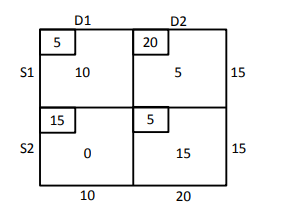
\includegraphics[width=0.75\columnwidth]{chapters/10/7/2/4/figs/fig.png}
 \end{center}
\caption{}
\label{fig:10/7/2/4Fig1}
\end{figure}
\fi

\item Find the position vector of the mid point of the vector joining the points $\vec{P}$(2, 3, 4)
and $\vec{Q}$(4, 1, –2).
\\
\solution
		\begin{enumerate}[label=\thesubsection.\arabic*,ref=\thesubsection.\theenumi]
\item Find the coordinates of the point which divides the join of $(-1,7) $ and $ (4,-3)$ in the ratio 2:3.
	\\
		\solution
	\input{chapters/10/7/2/1/section.tex}
\item Find the coordinates of the point $\vec{R}$ on the line segment joining the points $\vec{P}(-1,3)$ and $\vec{Q}(2,5)$ such that $PR=\frac{3}{5}PQ$.
\item Find the ratio in which the point $\vec{P}\brak{\frac{3}{4},\frac{5}{12}}$ divides the line segment joining the points $\vec{A}\brak{\frac{1}{2},\frac{3}{2}}$ and $ \vec{B}(2,-5)$.
\item Find the coordinates of the point which divides the line segment joining the points $(4,-3)$ and $(8,5)$ in the ratio $3:1$ internally.
\item Find the coordinates of the point $\vec{P}$ on $AD$ such that $AP : PD = 2 : 1$.
\item If the point $\vec{P} (2, 1)$ lies on the line segment joining points $\vec{A} (4, 2)$  and $ \vec{B} (8, 4)$,
then
\begin{enumerate}
	\item $AP =\frac{1}{3}{AB}$ 
\item ${AP}={PE}$
\item ${PB}=\frac{1}{3}{AB}$
\item${AP}=\frac{1}{2}{AB}$
 \end{enumerate}
\item Find the ratio in which the line segment joining the points $(-3,10)$  and  $(6,-8)$  is divided by $ (-1,6)$.
	\\
		\solution
	\input{chapters/10/7/2/4/section.tex}
\item Find the position vector of the mid point of the vector joining the points $\vec{P}$(2, 3, 4)
and $\vec{Q}$(4, 1, –2).
\\
\solution
		\input{chapters/12/10/2/16/section.tex}
\item Let $\vec{A}(4, 2), \vec{B}(6, 5)$  and $ \vec{C}(1, 4)$ be the vertices of $\triangle ABC$.
\begin{enumerate}
\item If $\vec{A}$ and  $\vec{B}$ are $(-2,-2)$ and  $(2,-4)$, respectively, find the coordinates of $\vec{P}$ such that $AP= \frac {3}{7}AB$  and $ \vec{P}$ lies on the line segment $AB$.
	\\
		\solution
	\input{chapters/10/7/2/8/section.tex}
\item Find the coordinates of the points which divide the line segment joining $A(-2,2)$  and  $\vec{B}(2,8)$ into four equal parts.
	\\
		\solution
	\input{chapters/10/7/2/9/section.tex}
\item In what ratio does the point $(-4,6)$ divide the line segment joining the points $\vec{A}(-6,0)$ and $\vec{B}(3,-8)$?
\item Given that $\vec{P}(3,2,-4), \vec{Q}(5,4,-6)$ and $\vec{R}(9,8,-10)$ are collinear. Find the ratio in which $\vec{Q}$ divides $PR$.
\item Points $\vec{A}(-6,10),\vec{B}(-4,6)$  and  $\vec{C}(3,-8)$ are collinear such that $AB=  \frac{2}{9}AC$.
\item The point which divides the line segment joining the points $\vec{P} (7, –6) $  and  $\vec{Q}(3, 4)$ in the 
ratio 1 : 2 internally lies in  which quadrant?
\item Find the coordinates of the points of trisection of the line segment joining $(4,-1)$  and  $(-2,3)$.
	\\
		\solution
	\input{chapters/10/7/2/2/section.tex}
\item Find the coordinates of the points which trisect the line segment joining the points $\vec{P}(4,2,-6)$ and $\vec{Q}(10,-16,6)$.
\item Find the coordinates of the points of trisection (i.e. points dividing to three equal parts) of the line segment joining the points $\vec{A}(2,-2)$ and $\vec{B}(-7,4)$.
\item Point $\vec{P}(5,-3)$ is one of the two points of trisection of line segment joining the points $\vec{A}(7,-2)$ and $\vec{B}(1,-5)$
\item Find the position vector of a point $\vec{R}$ which divides the line joining two points $\vec{P}$
and $\vec{Q}$ whose position vectors are $\hat{i}+2\hat{j}-\hat{k}$ and $-\hat{i}+\hat{j}+\hat{k}$ respectively, in the
ratio 2 : 1
\begin{enumerate}
    \item  internally
    \item  externally
\end{enumerate}
%\solution
%		\input{chapters/12/10/2/15/section.tex}
\item Find the coordinates of the point which divides the line segment joining the points which divides the line segment joining  the points $(-2,3,5)$ and $(1,-4,6)$ in the ratio 
\begin{enumerate}
\item $2:3$ internally,
\item $2:3$ externally
\end{enumerate}
\item Find the coordinates of the point which divides the line segment joining the points $(1,-2,3)$ and $(3,4,-5)$ in the ratio $2:3$
\begin{enumerate}
\item internally, and
\item externally
\end{enumerate}
\item Consider two points $\vec{P}$ and $\vec{Q}$ with position vectors $\overrightarrow{OP} = 3\overrightarrow{a}-2\overrightarrow{b}$ and $\overrightarrow{OQ}=\overrightarrow{a}+\overrightarrow{b}$. Find the position vector of a point $\vec{R}$ which divides the line joining $\vec{P}$ and $\vec{Q}$ in the ratio $2:1$, 
\begin{enumerate}
\item internally, and 
\item externally.
\end{enumerate}
\item The median from $\vec{A}$ meets $BC$ at $\vec{D}$. Find the coordinates of the point $\vec{D}$.
\item Find the coordinates of points $\vec{Q}$ and $\vec{R}$ on medians $BE$ and $CF$ respectively such that $BQ : QE = 2 : 1$  and  $CR : RF = 2 : 1$.
\item What do you observe?
\item If $\vec{A}, \vec{B}$ and $\vec{C}$  are the vertices of $\triangle ABC$, find the coordinates of the centroid of the triangle.
\end{enumerate}
\solution
	\input{chapters/10/7/4/7/section.tex}
\item If $\vec{P}(9a-2,-b)$ divides line segment joining $\vec{A}(3a+1,-3)$ and $\vec{B}(8a,5)$ in the ratio 3:1, find the values of $a$ and $b$.
\item Find the position vector of a point $\vec{R}$ which divides the line joining two points $\vec{P}$ and $\vec{Q}$ whose position vectors are $2\vec{a}+\vec{b}$ and $\vec{a}-3\vec{b}$ externally in the ratio $1:2$.
\item The position vector of the point which divides the join of points 2$\vec{a}$-3$\vec{b}$ $\text{and}$ $\vec{a}+\vec{b}$ in the ratio 3:1 is \rule{1cm}{0.1pt}.
\item If $\vec{a}$ and $\vec{b}$ are the postion vectors of $\vec{A}$ and $\vec{B}$, respectively, find the position vector of a point $\vec{C}$ in $BA$ produced such that $BC=1.5BA$.
\item Find the position vector of a point $\vec{R}$ which divides the line joining two points $\vec{P}$ and $\vec{Q}$ whose position vectors are $(2\vec{a}+\vec{b})$ and $(\vec{a}-3\vec{b})$
externally in the ratio 1 : 2. Also, show that $\vec{P}$ is the mid point of the line segment $RQ$.
\end{enumerate}

\item Let $\vec{A}(4, 2), \vec{B}(6, 5)$  and $ \vec{C}(1, 4)$ be the vertices of $\triangle ABC$.
\begin{enumerate}
\item If $\vec{A}$ and  $\vec{B}$ are $(-2,-2)$ and  $(2,-4)$, respectively, find the coordinates of $\vec{P}$ such that $AP= \frac {3}{7}AB$  and $ \vec{P}$ lies on the line segment $AB$.
	\\
		\solution
	\begin{enumerate}[label=\thesubsection.\arabic*,ref=\thesubsection.\theenumi]
\item Find the coordinates of the point which divides the join of $(-1,7) $ and $ (4,-3)$ in the ratio 2:3.
	\\
		\solution
	\input{chapters/10/7/2/1/section.tex}
\item Find the coordinates of the point $\vec{R}$ on the line segment joining the points $\vec{P}(-1,3)$ and $\vec{Q}(2,5)$ such that $PR=\frac{3}{5}PQ$.
\item Find the ratio in which the point $\vec{P}\brak{\frac{3}{4},\frac{5}{12}}$ divides the line segment joining the points $\vec{A}\brak{\frac{1}{2},\frac{3}{2}}$ and $ \vec{B}(2,-5)$.
\item Find the coordinates of the point which divides the line segment joining the points $(4,-3)$ and $(8,5)$ in the ratio $3:1$ internally.
\item Find the coordinates of the point $\vec{P}$ on $AD$ such that $AP : PD = 2 : 1$.
\item If the point $\vec{P} (2, 1)$ lies on the line segment joining points $\vec{A} (4, 2)$  and $ \vec{B} (8, 4)$,
then
\begin{enumerate}
	\item $AP =\frac{1}{3}{AB}$ 
\item ${AP}={PE}$
\item ${PB}=\frac{1}{3}{AB}$
\item${AP}=\frac{1}{2}{AB}$
 \end{enumerate}
\item Find the ratio in which the line segment joining the points $(-3,10)$  and  $(6,-8)$  is divided by $ (-1,6)$.
	\\
		\solution
	\input{chapters/10/7/2/4/section.tex}
\item Find the position vector of the mid point of the vector joining the points $\vec{P}$(2, 3, 4)
and $\vec{Q}$(4, 1, –2).
\\
\solution
		\input{chapters/12/10/2/16/section.tex}
\item Let $\vec{A}(4, 2), \vec{B}(6, 5)$  and $ \vec{C}(1, 4)$ be the vertices of $\triangle ABC$.
\begin{enumerate}
\item If $\vec{A}$ and  $\vec{B}$ are $(-2,-2)$ and  $(2,-4)$, respectively, find the coordinates of $\vec{P}$ such that $AP= \frac {3}{7}AB$  and $ \vec{P}$ lies on the line segment $AB$.
	\\
		\solution
	\input{chapters/10/7/2/8/section.tex}
\item Find the coordinates of the points which divide the line segment joining $A(-2,2)$  and  $\vec{B}(2,8)$ into four equal parts.
	\\
		\solution
	\input{chapters/10/7/2/9/section.tex}
\item In what ratio does the point $(-4,6)$ divide the line segment joining the points $\vec{A}(-6,0)$ and $\vec{B}(3,-8)$?
\item Given that $\vec{P}(3,2,-4), \vec{Q}(5,4,-6)$ and $\vec{R}(9,8,-10)$ are collinear. Find the ratio in which $\vec{Q}$ divides $PR$.
\item Points $\vec{A}(-6,10),\vec{B}(-4,6)$  and  $\vec{C}(3,-8)$ are collinear such that $AB=  \frac{2}{9}AC$.
\item The point which divides the line segment joining the points $\vec{P} (7, –6) $  and  $\vec{Q}(3, 4)$ in the 
ratio 1 : 2 internally lies in  which quadrant?
\item Find the coordinates of the points of trisection of the line segment joining $(4,-1)$  and  $(-2,3)$.
	\\
		\solution
	\input{chapters/10/7/2/2/section.tex}
\item Find the coordinates of the points which trisect the line segment joining the points $\vec{P}(4,2,-6)$ and $\vec{Q}(10,-16,6)$.
\item Find the coordinates of the points of trisection (i.e. points dividing to three equal parts) of the line segment joining the points $\vec{A}(2,-2)$ and $\vec{B}(-7,4)$.
\item Point $\vec{P}(5,-3)$ is one of the two points of trisection of line segment joining the points $\vec{A}(7,-2)$ and $\vec{B}(1,-5)$
\item Find the position vector of a point $\vec{R}$ which divides the line joining two points $\vec{P}$
and $\vec{Q}$ whose position vectors are $\hat{i}+2\hat{j}-\hat{k}$ and $-\hat{i}+\hat{j}+\hat{k}$ respectively, in the
ratio 2 : 1
\begin{enumerate}
    \item  internally
    \item  externally
\end{enumerate}
%\solution
%		\input{chapters/12/10/2/15/section.tex}
\item Find the coordinates of the point which divides the line segment joining the points which divides the line segment joining  the points $(-2,3,5)$ and $(1,-4,6)$ in the ratio 
\begin{enumerate}
\item $2:3$ internally,
\item $2:3$ externally
\end{enumerate}
\item Find the coordinates of the point which divides the line segment joining the points $(1,-2,3)$ and $(3,4,-5)$ in the ratio $2:3$
\begin{enumerate}
\item internally, and
\item externally
\end{enumerate}
\item Consider two points $\vec{P}$ and $\vec{Q}$ with position vectors $\overrightarrow{OP} = 3\overrightarrow{a}-2\overrightarrow{b}$ and $\overrightarrow{OQ}=\overrightarrow{a}+\overrightarrow{b}$. Find the position vector of a point $\vec{R}$ which divides the line joining $\vec{P}$ and $\vec{Q}$ in the ratio $2:1$, 
\begin{enumerate}
\item internally, and 
\item externally.
\end{enumerate}
\item The median from $\vec{A}$ meets $BC$ at $\vec{D}$. Find the coordinates of the point $\vec{D}$.
\item Find the coordinates of points $\vec{Q}$ and $\vec{R}$ on medians $BE$ and $CF$ respectively such that $BQ : QE = 2 : 1$  and  $CR : RF = 2 : 1$.
\item What do you observe?
\item If $\vec{A}, \vec{B}$ and $\vec{C}$  are the vertices of $\triangle ABC$, find the coordinates of the centroid of the triangle.
\end{enumerate}
\solution
	\input{chapters/10/7/4/7/section.tex}
\item If $\vec{P}(9a-2,-b)$ divides line segment joining $\vec{A}(3a+1,-3)$ and $\vec{B}(8a,5)$ in the ratio 3:1, find the values of $a$ and $b$.
\item Find the position vector of a point $\vec{R}$ which divides the line joining two points $\vec{P}$ and $\vec{Q}$ whose position vectors are $2\vec{a}+\vec{b}$ and $\vec{a}-3\vec{b}$ externally in the ratio $1:2$.
\item The position vector of the point which divides the join of points 2$\vec{a}$-3$\vec{b}$ $\text{and}$ $\vec{a}+\vec{b}$ in the ratio 3:1 is \rule{1cm}{0.1pt}.
\item If $\vec{a}$ and $\vec{b}$ are the postion vectors of $\vec{A}$ and $\vec{B}$, respectively, find the position vector of a point $\vec{C}$ in $BA$ produced such that $BC=1.5BA$.
\item Find the position vector of a point $\vec{R}$ which divides the line joining two points $\vec{P}$ and $\vec{Q}$ whose position vectors are $(2\vec{a}+\vec{b})$ and $(\vec{a}-3\vec{b})$
externally in the ratio 1 : 2. Also, show that $\vec{P}$ is the mid point of the line segment $RQ$.
\end{enumerate}

\item Find the coordinates of the points which divide the line segment joining $A(-2,2)$  and  $\vec{B}(2,8)$ into four equal parts.
	\\
		\solution
	\begin{enumerate}[label=\thesubsection.\arabic*,ref=\thesubsection.\theenumi]
\item Find the coordinates of the point which divides the join of $(-1,7) $ and $ (4,-3)$ in the ratio 2:3.
	\\
		\solution
	\input{chapters/10/7/2/1/section.tex}
\item Find the coordinates of the point $\vec{R}$ on the line segment joining the points $\vec{P}(-1,3)$ and $\vec{Q}(2,5)$ such that $PR=\frac{3}{5}PQ$.
\item Find the ratio in which the point $\vec{P}\brak{\frac{3}{4},\frac{5}{12}}$ divides the line segment joining the points $\vec{A}\brak{\frac{1}{2},\frac{3}{2}}$ and $ \vec{B}(2,-5)$.
\item Find the coordinates of the point which divides the line segment joining the points $(4,-3)$ and $(8,5)$ in the ratio $3:1$ internally.
\item Find the coordinates of the point $\vec{P}$ on $AD$ such that $AP : PD = 2 : 1$.
\item If the point $\vec{P} (2, 1)$ lies on the line segment joining points $\vec{A} (4, 2)$  and $ \vec{B} (8, 4)$,
then
\begin{enumerate}
	\item $AP =\frac{1}{3}{AB}$ 
\item ${AP}={PE}$
\item ${PB}=\frac{1}{3}{AB}$
\item${AP}=\frac{1}{2}{AB}$
 \end{enumerate}
\item Find the ratio in which the line segment joining the points $(-3,10)$  and  $(6,-8)$  is divided by $ (-1,6)$.
	\\
		\solution
	\input{chapters/10/7/2/4/section.tex}
\item Find the position vector of the mid point of the vector joining the points $\vec{P}$(2, 3, 4)
and $\vec{Q}$(4, 1, –2).
\\
\solution
		\input{chapters/12/10/2/16/section.tex}
\item Let $\vec{A}(4, 2), \vec{B}(6, 5)$  and $ \vec{C}(1, 4)$ be the vertices of $\triangle ABC$.
\begin{enumerate}
\item If $\vec{A}$ and  $\vec{B}$ are $(-2,-2)$ and  $(2,-4)$, respectively, find the coordinates of $\vec{P}$ such that $AP= \frac {3}{7}AB$  and $ \vec{P}$ lies on the line segment $AB$.
	\\
		\solution
	\input{chapters/10/7/2/8/section.tex}
\item Find the coordinates of the points which divide the line segment joining $A(-2,2)$  and  $\vec{B}(2,8)$ into four equal parts.
	\\
		\solution
	\input{chapters/10/7/2/9/section.tex}
\item In what ratio does the point $(-4,6)$ divide the line segment joining the points $\vec{A}(-6,0)$ and $\vec{B}(3,-8)$?
\item Given that $\vec{P}(3,2,-4), \vec{Q}(5,4,-6)$ and $\vec{R}(9,8,-10)$ are collinear. Find the ratio in which $\vec{Q}$ divides $PR$.
\item Points $\vec{A}(-6,10),\vec{B}(-4,6)$  and  $\vec{C}(3,-8)$ are collinear such that $AB=  \frac{2}{9}AC$.
\item The point which divides the line segment joining the points $\vec{P} (7, –6) $  and  $\vec{Q}(3, 4)$ in the 
ratio 1 : 2 internally lies in  which quadrant?
\item Find the coordinates of the points of trisection of the line segment joining $(4,-1)$  and  $(-2,3)$.
	\\
		\solution
	\input{chapters/10/7/2/2/section.tex}
\item Find the coordinates of the points which trisect the line segment joining the points $\vec{P}(4,2,-6)$ and $\vec{Q}(10,-16,6)$.
\item Find the coordinates of the points of trisection (i.e. points dividing to three equal parts) of the line segment joining the points $\vec{A}(2,-2)$ and $\vec{B}(-7,4)$.
\item Point $\vec{P}(5,-3)$ is one of the two points of trisection of line segment joining the points $\vec{A}(7,-2)$ and $\vec{B}(1,-5)$
\item Find the position vector of a point $\vec{R}$ which divides the line joining two points $\vec{P}$
and $\vec{Q}$ whose position vectors are $\hat{i}+2\hat{j}-\hat{k}$ and $-\hat{i}+\hat{j}+\hat{k}$ respectively, in the
ratio 2 : 1
\begin{enumerate}
    \item  internally
    \item  externally
\end{enumerate}
%\solution
%		\input{chapters/12/10/2/15/section.tex}
\item Find the coordinates of the point which divides the line segment joining the points which divides the line segment joining  the points $(-2,3,5)$ and $(1,-4,6)$ in the ratio 
\begin{enumerate}
\item $2:3$ internally,
\item $2:3$ externally
\end{enumerate}
\item Find the coordinates of the point which divides the line segment joining the points $(1,-2,3)$ and $(3,4,-5)$ in the ratio $2:3$
\begin{enumerate}
\item internally, and
\item externally
\end{enumerate}
\item Consider two points $\vec{P}$ and $\vec{Q}$ with position vectors $\overrightarrow{OP} = 3\overrightarrow{a}-2\overrightarrow{b}$ and $\overrightarrow{OQ}=\overrightarrow{a}+\overrightarrow{b}$. Find the position vector of a point $\vec{R}$ which divides the line joining $\vec{P}$ and $\vec{Q}$ in the ratio $2:1$, 
\begin{enumerate}
\item internally, and 
\item externally.
\end{enumerate}
\item The median from $\vec{A}$ meets $BC$ at $\vec{D}$. Find the coordinates of the point $\vec{D}$.
\item Find the coordinates of points $\vec{Q}$ and $\vec{R}$ on medians $BE$ and $CF$ respectively such that $BQ : QE = 2 : 1$  and  $CR : RF = 2 : 1$.
\item What do you observe?
\item If $\vec{A}, \vec{B}$ and $\vec{C}$  are the vertices of $\triangle ABC$, find the coordinates of the centroid of the triangle.
\end{enumerate}
\solution
	\input{chapters/10/7/4/7/section.tex}
\item If $\vec{P}(9a-2,-b)$ divides line segment joining $\vec{A}(3a+1,-3)$ and $\vec{B}(8a,5)$ in the ratio 3:1, find the values of $a$ and $b$.
\item Find the position vector of a point $\vec{R}$ which divides the line joining two points $\vec{P}$ and $\vec{Q}$ whose position vectors are $2\vec{a}+\vec{b}$ and $\vec{a}-3\vec{b}$ externally in the ratio $1:2$.
\item The position vector of the point which divides the join of points 2$\vec{a}$-3$\vec{b}$ $\text{and}$ $\vec{a}+\vec{b}$ in the ratio 3:1 is \rule{1cm}{0.1pt}.
\item If $\vec{a}$ and $\vec{b}$ are the postion vectors of $\vec{A}$ and $\vec{B}$, respectively, find the position vector of a point $\vec{C}$ in $BA$ produced such that $BC=1.5BA$.
\item Find the position vector of a point $\vec{R}$ which divides the line joining two points $\vec{P}$ and $\vec{Q}$ whose position vectors are $(2\vec{a}+\vec{b})$ and $(\vec{a}-3\vec{b})$
externally in the ratio 1 : 2. Also, show that $\vec{P}$ is the mid point of the line segment $RQ$.
\end{enumerate}

\item In what ratio does the point $(-4,6)$ divide the line segment joining the points $\vec{A}(-6,0)$ and $\vec{B}(3,-8)$?
\item Given that $\vec{P}(3,2,-4), \vec{Q}(5,4,-6)$ and $\vec{R}(9,8,-10)$ are collinear. Find the ratio in which $\vec{Q}$ divides $PR$.
\item Points $\vec{A}(-6,10),\vec{B}(-4,6)$  and  $\vec{C}(3,-8)$ are collinear such that $AB=  \frac{2}{9}AC$.
\item The point which divides the line segment joining the points $\vec{P} (7, –6) $  and  $\vec{Q}(3, 4)$ in the 
ratio 1 : 2 internally lies in  which quadrant?
\item Find the coordinates of the points of trisection of the line segment joining $(4,-1)$  and  $(-2,3)$.
	\\
		\solution
	Using section formula,
\begin{align}
\vec{R}=\frac{1}{1+\frac{1}{2}}\brak{\myvec{4\\-1}+\frac{1}{2}\myvec{-2\\3}}
=\myvec{2\\ \frac{1}{3}}\\
\vec{S}=\frac{1}{1+\frac{2}{1}}\brak{\myvec{4\\-1}+\frac{2}{1}\myvec{-2\\3}}
=\myvec{0\\ \frac{5}{3}}
\end{align}
which are the desired points of trisection.
\iffalse
See
		\figref{fig:chapters/10/7/2/2/Figure}
\begin{figure}[H]
\centering
\includegraphics[width=0.75\columnwidth]{chapters/10/7/2/2/figs/dj.pdf}
\caption{}
		\label{fig:chapters/10/7/2/2/Figure}
\end{figure}
\fi

\item Find the coordinates of the points which trisect the line segment joining the points $\vec{P}(4,2,-6)$ and $\vec{Q}(10,-16,6)$.
\item Find the coordinates of the points of trisection (i.e. points dividing to three equal parts) of the line segment joining the points $\vec{A}(2,-2)$ and $\vec{B}(-7,4)$.
\item Point $\vec{P}(5,-3)$ is one of the two points of trisection of line segment joining the points $\vec{A}(7,-2)$ and $\vec{B}(1,-5)$
\item Find the position vector of a point $\vec{R}$ which divides the line joining two points $\vec{P}$
and $\vec{Q}$ whose position vectors are $\hat{i}+2\hat{j}-\hat{k}$ and $-\hat{i}+\hat{j}+\hat{k}$ respectively, in the
ratio 2 : 1
\begin{enumerate}
    \item  internally
    \item  externally
\end{enumerate}
%\solution
%		\begin{enumerate}[label=\thesubsection.\arabic*,ref=\thesubsection.\theenumi]
\item Find the coordinates of the point which divides the join of $(-1,7) $ and $ (4,-3)$ in the ratio 2:3.
	\\
		\solution
	\input{chapters/10/7/2/1/section.tex}
\item Find the coordinates of the point $\vec{R}$ on the line segment joining the points $\vec{P}(-1,3)$ and $\vec{Q}(2,5)$ such that $PR=\frac{3}{5}PQ$.
\item Find the ratio in which the point $\vec{P}\brak{\frac{3}{4},\frac{5}{12}}$ divides the line segment joining the points $\vec{A}\brak{\frac{1}{2},\frac{3}{2}}$ and $ \vec{B}(2,-5)$.
\item Find the coordinates of the point which divides the line segment joining the points $(4,-3)$ and $(8,5)$ in the ratio $3:1$ internally.
\item Find the coordinates of the point $\vec{P}$ on $AD$ such that $AP : PD = 2 : 1$.
\item If the point $\vec{P} (2, 1)$ lies on the line segment joining points $\vec{A} (4, 2)$  and $ \vec{B} (8, 4)$,
then
\begin{enumerate}
	\item $AP =\frac{1}{3}{AB}$ 
\item ${AP}={PE}$
\item ${PB}=\frac{1}{3}{AB}$
\item${AP}=\frac{1}{2}{AB}$
 \end{enumerate}
\item Find the ratio in which the line segment joining the points $(-3,10)$  and  $(6,-8)$  is divided by $ (-1,6)$.
	\\
		\solution
	\input{chapters/10/7/2/4/section.tex}
\item Find the position vector of the mid point of the vector joining the points $\vec{P}$(2, 3, 4)
and $\vec{Q}$(4, 1, –2).
\\
\solution
		\input{chapters/12/10/2/16/section.tex}
\item Let $\vec{A}(4, 2), \vec{B}(6, 5)$  and $ \vec{C}(1, 4)$ be the vertices of $\triangle ABC$.
\begin{enumerate}
\item If $\vec{A}$ and  $\vec{B}$ are $(-2,-2)$ and  $(2,-4)$, respectively, find the coordinates of $\vec{P}$ such that $AP= \frac {3}{7}AB$  and $ \vec{P}$ lies on the line segment $AB$.
	\\
		\solution
	\input{chapters/10/7/2/8/section.tex}
\item Find the coordinates of the points which divide the line segment joining $A(-2,2)$  and  $\vec{B}(2,8)$ into four equal parts.
	\\
		\solution
	\input{chapters/10/7/2/9/section.tex}
\item In what ratio does the point $(-4,6)$ divide the line segment joining the points $\vec{A}(-6,0)$ and $\vec{B}(3,-8)$?
\item Given that $\vec{P}(3,2,-4), \vec{Q}(5,4,-6)$ and $\vec{R}(9,8,-10)$ are collinear. Find the ratio in which $\vec{Q}$ divides $PR$.
\item Points $\vec{A}(-6,10),\vec{B}(-4,6)$  and  $\vec{C}(3,-8)$ are collinear such that $AB=  \frac{2}{9}AC$.
\item The point which divides the line segment joining the points $\vec{P} (7, –6) $  and  $\vec{Q}(3, 4)$ in the 
ratio 1 : 2 internally lies in  which quadrant?
\item Find the coordinates of the points of trisection of the line segment joining $(4,-1)$  and  $(-2,3)$.
	\\
		\solution
	\input{chapters/10/7/2/2/section.tex}
\item Find the coordinates of the points which trisect the line segment joining the points $\vec{P}(4,2,-6)$ and $\vec{Q}(10,-16,6)$.
\item Find the coordinates of the points of trisection (i.e. points dividing to three equal parts) of the line segment joining the points $\vec{A}(2,-2)$ and $\vec{B}(-7,4)$.
\item Point $\vec{P}(5,-3)$ is one of the two points of trisection of line segment joining the points $\vec{A}(7,-2)$ and $\vec{B}(1,-5)$
\item Find the position vector of a point $\vec{R}$ which divides the line joining two points $\vec{P}$
and $\vec{Q}$ whose position vectors are $\hat{i}+2\hat{j}-\hat{k}$ and $-\hat{i}+\hat{j}+\hat{k}$ respectively, in the
ratio 2 : 1
\begin{enumerate}
    \item  internally
    \item  externally
\end{enumerate}
%\solution
%		\input{chapters/12/10/2/15/section.tex}
\item Find the coordinates of the point which divides the line segment joining the points which divides the line segment joining  the points $(-2,3,5)$ and $(1,-4,6)$ in the ratio 
\begin{enumerate}
\item $2:3$ internally,
\item $2:3$ externally
\end{enumerate}
\item Find the coordinates of the point which divides the line segment joining the points $(1,-2,3)$ and $(3,4,-5)$ in the ratio $2:3$
\begin{enumerate}
\item internally, and
\item externally
\end{enumerate}
\item Consider two points $\vec{P}$ and $\vec{Q}$ with position vectors $\overrightarrow{OP} = 3\overrightarrow{a}-2\overrightarrow{b}$ and $\overrightarrow{OQ}=\overrightarrow{a}+\overrightarrow{b}$. Find the position vector of a point $\vec{R}$ which divides the line joining $\vec{P}$ and $\vec{Q}$ in the ratio $2:1$, 
\begin{enumerate}
\item internally, and 
\item externally.
\end{enumerate}
\item The median from $\vec{A}$ meets $BC$ at $\vec{D}$. Find the coordinates of the point $\vec{D}$.
\item Find the coordinates of points $\vec{Q}$ and $\vec{R}$ on medians $BE$ and $CF$ respectively such that $BQ : QE = 2 : 1$  and  $CR : RF = 2 : 1$.
\item What do you observe?
\item If $\vec{A}, \vec{B}$ and $\vec{C}$  are the vertices of $\triangle ABC$, find the coordinates of the centroid of the triangle.
\end{enumerate}
\solution
	\input{chapters/10/7/4/7/section.tex}
\item If $\vec{P}(9a-2,-b)$ divides line segment joining $\vec{A}(3a+1,-3)$ and $\vec{B}(8a,5)$ in the ratio 3:1, find the values of $a$ and $b$.
\item Find the position vector of a point $\vec{R}$ which divides the line joining two points $\vec{P}$ and $\vec{Q}$ whose position vectors are $2\vec{a}+\vec{b}$ and $\vec{a}-3\vec{b}$ externally in the ratio $1:2$.
\item The position vector of the point which divides the join of points 2$\vec{a}$-3$\vec{b}$ $\text{and}$ $\vec{a}+\vec{b}$ in the ratio 3:1 is \rule{1cm}{0.1pt}.
\item If $\vec{a}$ and $\vec{b}$ are the postion vectors of $\vec{A}$ and $\vec{B}$, respectively, find the position vector of a point $\vec{C}$ in $BA$ produced such that $BC=1.5BA$.
\item Find the position vector of a point $\vec{R}$ which divides the line joining two points $\vec{P}$ and $\vec{Q}$ whose position vectors are $(2\vec{a}+\vec{b})$ and $(\vec{a}-3\vec{b})$
externally in the ratio 1 : 2. Also, show that $\vec{P}$ is the mid point of the line segment $RQ$.
\end{enumerate}

\item Find the coordinates of the point which divides the line segment joining the points which divides the line segment joining  the points $(-2,3,5)$ and $(1,-4,6)$ in the ratio 
\begin{enumerate}
\item $2:3$ internally,
\item $2:3$ externally
\end{enumerate}
\item Find the coordinates of the point which divides the line segment joining the points $(1,-2,3)$ and $(3,4,-5)$ in the ratio $2:3$
\begin{enumerate}
\item internally, and
\item externally
\end{enumerate}
\item Consider two points $\vec{P}$ and $\vec{Q}$ with position vectors $\overrightarrow{OP} = 3\overrightarrow{a}-2\overrightarrow{b}$ and $\overrightarrow{OQ}=\overrightarrow{a}+\overrightarrow{b}$. Find the position vector of a point $\vec{R}$ which divides the line joining $\vec{P}$ and $\vec{Q}$ in the ratio $2:1$, 
\begin{enumerate}
\item internally, and 
\item externally.
\end{enumerate}
\item The median from $\vec{A}$ meets $BC$ at $\vec{D}$. Find the coordinates of the point $\vec{D}$.
\item Find the coordinates of points $\vec{Q}$ and $\vec{R}$ on medians $BE$ and $CF$ respectively such that $BQ : QE = 2 : 1$  and  $CR : RF = 2 : 1$.
\item What do you observe?
\item If $\vec{A}, \vec{B}$ and $\vec{C}$  are the vertices of $\triangle ABC$, find the coordinates of the centroid of the triangle.
\end{enumerate}
\solution
	\begin{enumerate}[label=\thesubsection.\arabic*,ref=\thesubsection.\theenumi]
\item Find the coordinates of the point which divides the join of $(-1,7) $ and $ (4,-3)$ in the ratio 2:3.
	\\
		\solution
	\input{chapters/10/7/2/1/section.tex}
\item Find the coordinates of the point $\vec{R}$ on the line segment joining the points $\vec{P}(-1,3)$ and $\vec{Q}(2,5)$ such that $PR=\frac{3}{5}PQ$.
\item Find the ratio in which the point $\vec{P}\brak{\frac{3}{4},\frac{5}{12}}$ divides the line segment joining the points $\vec{A}\brak{\frac{1}{2},\frac{3}{2}}$ and $ \vec{B}(2,-5)$.
\item Find the coordinates of the point which divides the line segment joining the points $(4,-3)$ and $(8,5)$ in the ratio $3:1$ internally.
\item Find the coordinates of the point $\vec{P}$ on $AD$ such that $AP : PD = 2 : 1$.
\item If the point $\vec{P} (2, 1)$ lies on the line segment joining points $\vec{A} (4, 2)$  and $ \vec{B} (8, 4)$,
then
\begin{enumerate}
	\item $AP =\frac{1}{3}{AB}$ 
\item ${AP}={PE}$
\item ${PB}=\frac{1}{3}{AB}$
\item${AP}=\frac{1}{2}{AB}$
 \end{enumerate}
\item Find the ratio in which the line segment joining the points $(-3,10)$  and  $(6,-8)$  is divided by $ (-1,6)$.
	\\
		\solution
	\input{chapters/10/7/2/4/section.tex}
\item Find the position vector of the mid point of the vector joining the points $\vec{P}$(2, 3, 4)
and $\vec{Q}$(4, 1, –2).
\\
\solution
		\input{chapters/12/10/2/16/section.tex}
\item Let $\vec{A}(4, 2), \vec{B}(6, 5)$  and $ \vec{C}(1, 4)$ be the vertices of $\triangle ABC$.
\begin{enumerate}
\item If $\vec{A}$ and  $\vec{B}$ are $(-2,-2)$ and  $(2,-4)$, respectively, find the coordinates of $\vec{P}$ such that $AP= \frac {3}{7}AB$  and $ \vec{P}$ lies on the line segment $AB$.
	\\
		\solution
	\input{chapters/10/7/2/8/section.tex}
\item Find the coordinates of the points which divide the line segment joining $A(-2,2)$  and  $\vec{B}(2,8)$ into four equal parts.
	\\
		\solution
	\input{chapters/10/7/2/9/section.tex}
\item In what ratio does the point $(-4,6)$ divide the line segment joining the points $\vec{A}(-6,0)$ and $\vec{B}(3,-8)$?
\item Given that $\vec{P}(3,2,-4), \vec{Q}(5,4,-6)$ and $\vec{R}(9,8,-10)$ are collinear. Find the ratio in which $\vec{Q}$ divides $PR$.
\item Points $\vec{A}(-6,10),\vec{B}(-4,6)$  and  $\vec{C}(3,-8)$ are collinear such that $AB=  \frac{2}{9}AC$.
\item The point which divides the line segment joining the points $\vec{P} (7, –6) $  and  $\vec{Q}(3, 4)$ in the 
ratio 1 : 2 internally lies in  which quadrant?
\item Find the coordinates of the points of trisection of the line segment joining $(4,-1)$  and  $(-2,3)$.
	\\
		\solution
	\input{chapters/10/7/2/2/section.tex}
\item Find the coordinates of the points which trisect the line segment joining the points $\vec{P}(4,2,-6)$ and $\vec{Q}(10,-16,6)$.
\item Find the coordinates of the points of trisection (i.e. points dividing to three equal parts) of the line segment joining the points $\vec{A}(2,-2)$ and $\vec{B}(-7,4)$.
\item Point $\vec{P}(5,-3)$ is one of the two points of trisection of line segment joining the points $\vec{A}(7,-2)$ and $\vec{B}(1,-5)$
\item Find the position vector of a point $\vec{R}$ which divides the line joining two points $\vec{P}$
and $\vec{Q}$ whose position vectors are $\hat{i}+2\hat{j}-\hat{k}$ and $-\hat{i}+\hat{j}+\hat{k}$ respectively, in the
ratio 2 : 1
\begin{enumerate}
    \item  internally
    \item  externally
\end{enumerate}
%\solution
%		\input{chapters/12/10/2/15/section.tex}
\item Find the coordinates of the point which divides the line segment joining the points which divides the line segment joining  the points $(-2,3,5)$ and $(1,-4,6)$ in the ratio 
\begin{enumerate}
\item $2:3$ internally,
\item $2:3$ externally
\end{enumerate}
\item Find the coordinates of the point which divides the line segment joining the points $(1,-2,3)$ and $(3,4,-5)$ in the ratio $2:3$
\begin{enumerate}
\item internally, and
\item externally
\end{enumerate}
\item Consider two points $\vec{P}$ and $\vec{Q}$ with position vectors $\overrightarrow{OP} = 3\overrightarrow{a}-2\overrightarrow{b}$ and $\overrightarrow{OQ}=\overrightarrow{a}+\overrightarrow{b}$. Find the position vector of a point $\vec{R}$ which divides the line joining $\vec{P}$ and $\vec{Q}$ in the ratio $2:1$, 
\begin{enumerate}
\item internally, and 
\item externally.
\end{enumerate}
\item The median from $\vec{A}$ meets $BC$ at $\vec{D}$. Find the coordinates of the point $\vec{D}$.
\item Find the coordinates of points $\vec{Q}$ and $\vec{R}$ on medians $BE$ and $CF$ respectively such that $BQ : QE = 2 : 1$  and  $CR : RF = 2 : 1$.
\item What do you observe?
\item If $\vec{A}, \vec{B}$ and $\vec{C}$  are the vertices of $\triangle ABC$, find the coordinates of the centroid of the triangle.
\end{enumerate}
\solution
	\input{chapters/10/7/4/7/section.tex}
\item If $\vec{P}(9a-2,-b)$ divides line segment joining $\vec{A}(3a+1,-3)$ and $\vec{B}(8a,5)$ in the ratio 3:1, find the values of $a$ and $b$.
\item Find the position vector of a point $\vec{R}$ which divides the line joining two points $\vec{P}$ and $\vec{Q}$ whose position vectors are $2\vec{a}+\vec{b}$ and $\vec{a}-3\vec{b}$ externally in the ratio $1:2$.
\item The position vector of the point which divides the join of points 2$\vec{a}$-3$\vec{b}$ $\text{and}$ $\vec{a}+\vec{b}$ in the ratio 3:1 is \rule{1cm}{0.1pt}.
\item If $\vec{a}$ and $\vec{b}$ are the postion vectors of $\vec{A}$ and $\vec{B}$, respectively, find the position vector of a point $\vec{C}$ in $BA$ produced such that $BC=1.5BA$.
\item Find the position vector of a point $\vec{R}$ which divides the line joining two points $\vec{P}$ and $\vec{Q}$ whose position vectors are $(2\vec{a}+\vec{b})$ and $(\vec{a}-3\vec{b})$
externally in the ratio 1 : 2. Also, show that $\vec{P}$ is the mid point of the line segment $RQ$.
\end{enumerate}

\item If $\vec{P}(9a-2,-b)$ divides line segment joining $\vec{A}(3a+1,-3)$ and $\vec{B}(8a,5)$ in the ratio 3:1, find the values of $a$ and $b$.
\item Find the position vector of a point $\vec{R}$ which divides the line joining two points $\vec{P}$ and $\vec{Q}$ whose position vectors are $2\vec{a}+\vec{b}$ and $\vec{a}-3\vec{b}$ externally in the ratio $1:2$.
\item The position vector of the point which divides the join of points 2$\vec{a}$-3$\vec{b}$ $\text{and}$ $\vec{a}+\vec{b}$ in the ratio 3:1 is \rule{1cm}{0.1pt}.
\item If $\vec{a}$ and $\vec{b}$ are the postion vectors of $\vec{A}$ and $\vec{B}$, respectively, find the position vector of a point $\vec{C}$ in $BA$ produced such that $BC=1.5BA$.
\item Find the position vector of a point $\vec{R}$ which divides the line joining two points $\vec{P}$ and $\vec{Q}$ whose position vectors are $(2\vec{a}+\vec{b})$ and $(\vec{a}-3\vec{b})$
externally in the ratio 1 : 2. Also, show that $\vec{P}$ is the mid point of the line segment $RQ$.
\end{enumerate}

\item Find the coordinates of the point which divides the line segment joining the points which divides the line segment joining  the points $(-2,3,5)$ and $(1,-4,6)$ in the ratio 
\begin{enumerate}
\item $2:3$ internally,
\item $2:3$ externally
\end{enumerate}
\item Find the coordinates of the point which divides the line segment joining the points $(1,-2,3)$ and $(3,4,-5)$ in the ratio $2:3$
\begin{enumerate}
\item internally, and
\item externally
\end{enumerate}
\item Consider two points $\vec{P}$ and $\vec{Q}$ with position vectors $\overrightarrow{OP} = 3\overrightarrow{a}-2\overrightarrow{b}$ and $\overrightarrow{OQ}=\overrightarrow{a}+\overrightarrow{b}$. Find the position vector of a point $\vec{R}$ which divides the line joining $\vec{P}$ and $\vec{Q}$ in the ratio $2:1$, 
\begin{enumerate}
\item internally, and 
\item externally.
\end{enumerate}
\item The median from $\vec{A}$ meets $BC$ at $\vec{D}$. Find the coordinates of the point $\vec{D}$.
\item Find the coordinates of points $\vec{Q}$ and $\vec{R}$ on medians $BE$ and $CF$ respectively such that $BQ : QE = 2 : 1$  and  $CR : RF = 2 : 1$.
\item What do you observe?
\item If $\vec{A}, \vec{B}$ and $\vec{C}$  are the vertices of $\triangle ABC$, find the coordinates of the centroid of the triangle.
\end{enumerate}
\solution
	\begin{enumerate}[label=\thesubsection.\arabic*,ref=\thesubsection.\theenumi]
\item Find the coordinates of the point which divides the join of $(-1,7) $ and $ (4,-3)$ in the ratio 2:3.
	\\
		\solution
	\begin{enumerate}[label=\thesubsection.\arabic*,ref=\thesubsection.\theenumi]
\item Find the coordinates of the point which divides the join of $(-1,7) $ and $ (4,-3)$ in the ratio 2:3.
	\\
		\solution
	\input{chapters/10/7/2/1/section.tex}
\item Find the coordinates of the point $\vec{R}$ on the line segment joining the points $\vec{P}(-1,3)$ and $\vec{Q}(2,5)$ such that $PR=\frac{3}{5}PQ$.
\item Find the ratio in which the point $\vec{P}\brak{\frac{3}{4},\frac{5}{12}}$ divides the line segment joining the points $\vec{A}\brak{\frac{1}{2},\frac{3}{2}}$ and $ \vec{B}(2,-5)$.
\item Find the coordinates of the point which divides the line segment joining the points $(4,-3)$ and $(8,5)$ in the ratio $3:1$ internally.
\item Find the coordinates of the point $\vec{P}$ on $AD$ such that $AP : PD = 2 : 1$.
\item If the point $\vec{P} (2, 1)$ lies on the line segment joining points $\vec{A} (4, 2)$  and $ \vec{B} (8, 4)$,
then
\begin{enumerate}
	\item $AP =\frac{1}{3}{AB}$ 
\item ${AP}={PE}$
\item ${PB}=\frac{1}{3}{AB}$
\item${AP}=\frac{1}{2}{AB}$
 \end{enumerate}
\item Find the ratio in which the line segment joining the points $(-3,10)$  and  $(6,-8)$  is divided by $ (-1,6)$.
	\\
		\solution
	\input{chapters/10/7/2/4/section.tex}
\item Find the position vector of the mid point of the vector joining the points $\vec{P}$(2, 3, 4)
and $\vec{Q}$(4, 1, –2).
\\
\solution
		\input{chapters/12/10/2/16/section.tex}
\item Let $\vec{A}(4, 2), \vec{B}(6, 5)$  and $ \vec{C}(1, 4)$ be the vertices of $\triangle ABC$.
\begin{enumerate}
\item If $\vec{A}$ and  $\vec{B}$ are $(-2,-2)$ and  $(2,-4)$, respectively, find the coordinates of $\vec{P}$ such that $AP= \frac {3}{7}AB$  and $ \vec{P}$ lies on the line segment $AB$.
	\\
		\solution
	\input{chapters/10/7/2/8/section.tex}
\item Find the coordinates of the points which divide the line segment joining $A(-2,2)$  and  $\vec{B}(2,8)$ into four equal parts.
	\\
		\solution
	\input{chapters/10/7/2/9/section.tex}
\item In what ratio does the point $(-4,6)$ divide the line segment joining the points $\vec{A}(-6,0)$ and $\vec{B}(3,-8)$?
\item Given that $\vec{P}(3,2,-4), \vec{Q}(5,4,-6)$ and $\vec{R}(9,8,-10)$ are collinear. Find the ratio in which $\vec{Q}$ divides $PR$.
\item Points $\vec{A}(-6,10),\vec{B}(-4,6)$  and  $\vec{C}(3,-8)$ are collinear such that $AB=  \frac{2}{9}AC$.
\item The point which divides the line segment joining the points $\vec{P} (7, –6) $  and  $\vec{Q}(3, 4)$ in the 
ratio 1 : 2 internally lies in  which quadrant?
\item Find the coordinates of the points of trisection of the line segment joining $(4,-1)$  and  $(-2,3)$.
	\\
		\solution
	\input{chapters/10/7/2/2/section.tex}
\item Find the coordinates of the points which trisect the line segment joining the points $\vec{P}(4,2,-6)$ and $\vec{Q}(10,-16,6)$.
\item Find the coordinates of the points of trisection (i.e. points dividing to three equal parts) of the line segment joining the points $\vec{A}(2,-2)$ and $\vec{B}(-7,4)$.
\item Point $\vec{P}(5,-3)$ is one of the two points of trisection of line segment joining the points $\vec{A}(7,-2)$ and $\vec{B}(1,-5)$
\item Find the position vector of a point $\vec{R}$ which divides the line joining two points $\vec{P}$
and $\vec{Q}$ whose position vectors are $\hat{i}+2\hat{j}-\hat{k}$ and $-\hat{i}+\hat{j}+\hat{k}$ respectively, in the
ratio 2 : 1
\begin{enumerate}
    \item  internally
    \item  externally
\end{enumerate}
%\solution
%		\input{chapters/12/10/2/15/section.tex}
\item Find the coordinates of the point which divides the line segment joining the points which divides the line segment joining  the points $(-2,3,5)$ and $(1,-4,6)$ in the ratio 
\begin{enumerate}
\item $2:3$ internally,
\item $2:3$ externally
\end{enumerate}
\item Find the coordinates of the point which divides the line segment joining the points $(1,-2,3)$ and $(3,4,-5)$ in the ratio $2:3$
\begin{enumerate}
\item internally, and
\item externally
\end{enumerate}
\item Consider two points $\vec{P}$ and $\vec{Q}$ with position vectors $\overrightarrow{OP} = 3\overrightarrow{a}-2\overrightarrow{b}$ and $\overrightarrow{OQ}=\overrightarrow{a}+\overrightarrow{b}$. Find the position vector of a point $\vec{R}$ which divides the line joining $\vec{P}$ and $\vec{Q}$ in the ratio $2:1$, 
\begin{enumerate}
\item internally, and 
\item externally.
\end{enumerate}
\item The median from $\vec{A}$ meets $BC$ at $\vec{D}$. Find the coordinates of the point $\vec{D}$.
\item Find the coordinates of points $\vec{Q}$ and $\vec{R}$ on medians $BE$ and $CF$ respectively such that $BQ : QE = 2 : 1$  and  $CR : RF = 2 : 1$.
\item What do you observe?
\item If $\vec{A}, \vec{B}$ and $\vec{C}$  are the vertices of $\triangle ABC$, find the coordinates of the centroid of the triangle.
\end{enumerate}
\solution
	\input{chapters/10/7/4/7/section.tex}
\item If $\vec{P}(9a-2,-b)$ divides line segment joining $\vec{A}(3a+1,-3)$ and $\vec{B}(8a,5)$ in the ratio 3:1, find the values of $a$ and $b$.
\item Find the position vector of a point $\vec{R}$ which divides the line joining two points $\vec{P}$ and $\vec{Q}$ whose position vectors are $2\vec{a}+\vec{b}$ and $\vec{a}-3\vec{b}$ externally in the ratio $1:2$.
\item The position vector of the point which divides the join of points 2$\vec{a}$-3$\vec{b}$ $\text{and}$ $\vec{a}+\vec{b}$ in the ratio 3:1 is \rule{1cm}{0.1pt}.
\item If $\vec{a}$ and $\vec{b}$ are the postion vectors of $\vec{A}$ and $\vec{B}$, respectively, find the position vector of a point $\vec{C}$ in $BA$ produced such that $BC=1.5BA$.
\item Find the position vector of a point $\vec{R}$ which divides the line joining two points $\vec{P}$ and $\vec{Q}$ whose position vectors are $(2\vec{a}+\vec{b})$ and $(\vec{a}-3\vec{b})$
externally in the ratio 1 : 2. Also, show that $\vec{P}$ is the mid point of the line segment $RQ$.
\end{enumerate}

\item Find the coordinates of the point $\vec{R}$ on the line segment joining the points $\vec{P}(-1,3)$ and $\vec{Q}(2,5)$ such that $PR=\frac{3}{5}PQ$.
\item Find the ratio in which the point $\vec{P}\brak{\frac{3}{4},\frac{5}{12}}$ divides the line segment joining the points $\vec{A}\brak{\frac{1}{2},\frac{3}{2}}$ and $ \vec{B}(2,-5)$.
\item Find the coordinates of the point which divides the line segment joining the points $(4,-3)$ and $(8,5)$ in the ratio $3:1$ internally.
\item Find the coordinates of the point $\vec{P}$ on $AD$ such that $AP : PD = 2 : 1$.
\item If the point $\vec{P} (2, 1)$ lies on the line segment joining points $\vec{A} (4, 2)$  and $ \vec{B} (8, 4)$,
then
\begin{enumerate}
	\item $AP =\frac{1}{3}{AB}$ 
\item ${AP}={PE}$
\item ${PB}=\frac{1}{3}{AB}$
\item${AP}=\frac{1}{2}{AB}$
 \end{enumerate}
\item Find the ratio in which the line segment joining the points $(-3,10)$  and  $(6,-8)$  is divided by $ (-1,6)$.
	\\
		\solution
	\iffalse
Using section formula,
\begin{align}
         \myvec{-1\\6} &=\frac{{\myvec{-3\\10}+k\myvec{6\\-8}}}{1+k}\\
	 \implies 7k\myvec{1 \\ -2} &= 2\myvec{1 \\ -2}
	 \\
	 \text{or, } k &= \frac{2}{7}.
\end{align}
\fi
In 
			\eqref{eq:section_formula-k}, substituting
			\begin{align}
				\vec{B} &= \myvec{-3\\10}, \vec{C} = \myvec{6\\-8}, \vec{D} = \myvec{-1\\6},
				\\
				k &= \frac{\myvec{-2 & 4}\myvec{-7 \\ 14}}{\norm{\myvec{-7 \\ 14}}^2} = \frac{2}{7}
			\end{align}
\iffalse
See \figref{fig:10/7/2/4Fig1}.
\begin{figure}[H]
 \begin{center}
  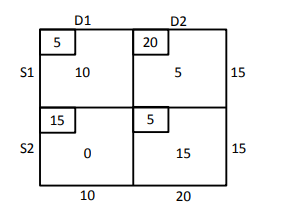
\includegraphics[width=0.75\columnwidth]{chapters/10/7/2/4/figs/fig.png}
 \end{center}
\caption{}
\label{fig:10/7/2/4Fig1}
\end{figure}
\fi

\item Find the position vector of the mid point of the vector joining the points $\vec{P}$(2, 3, 4)
and $\vec{Q}$(4, 1, –2).
\\
\solution
		\begin{enumerate}[label=\thesubsection.\arabic*,ref=\thesubsection.\theenumi]
\item Find the coordinates of the point which divides the join of $(-1,7) $ and $ (4,-3)$ in the ratio 2:3.
	\\
		\solution
	\input{chapters/10/7/2/1/section.tex}
\item Find the coordinates of the point $\vec{R}$ on the line segment joining the points $\vec{P}(-1,3)$ and $\vec{Q}(2,5)$ such that $PR=\frac{3}{5}PQ$.
\item Find the ratio in which the point $\vec{P}\brak{\frac{3}{4},\frac{5}{12}}$ divides the line segment joining the points $\vec{A}\brak{\frac{1}{2},\frac{3}{2}}$ and $ \vec{B}(2,-5)$.
\item Find the coordinates of the point which divides the line segment joining the points $(4,-3)$ and $(8,5)$ in the ratio $3:1$ internally.
\item Find the coordinates of the point $\vec{P}$ on $AD$ such that $AP : PD = 2 : 1$.
\item If the point $\vec{P} (2, 1)$ lies on the line segment joining points $\vec{A} (4, 2)$  and $ \vec{B} (8, 4)$,
then
\begin{enumerate}
	\item $AP =\frac{1}{3}{AB}$ 
\item ${AP}={PE}$
\item ${PB}=\frac{1}{3}{AB}$
\item${AP}=\frac{1}{2}{AB}$
 \end{enumerate}
\item Find the ratio in which the line segment joining the points $(-3,10)$  and  $(6,-8)$  is divided by $ (-1,6)$.
	\\
		\solution
	\input{chapters/10/7/2/4/section.tex}
\item Find the position vector of the mid point of the vector joining the points $\vec{P}$(2, 3, 4)
and $\vec{Q}$(4, 1, –2).
\\
\solution
		\input{chapters/12/10/2/16/section.tex}
\item Let $\vec{A}(4, 2), \vec{B}(6, 5)$  and $ \vec{C}(1, 4)$ be the vertices of $\triangle ABC$.
\begin{enumerate}
\item If $\vec{A}$ and  $\vec{B}$ are $(-2,-2)$ and  $(2,-4)$, respectively, find the coordinates of $\vec{P}$ such that $AP= \frac {3}{7}AB$  and $ \vec{P}$ lies on the line segment $AB$.
	\\
		\solution
	\input{chapters/10/7/2/8/section.tex}
\item Find the coordinates of the points which divide the line segment joining $A(-2,2)$  and  $\vec{B}(2,8)$ into four equal parts.
	\\
		\solution
	\input{chapters/10/7/2/9/section.tex}
\item In what ratio does the point $(-4,6)$ divide the line segment joining the points $\vec{A}(-6,0)$ and $\vec{B}(3,-8)$?
\item Given that $\vec{P}(3,2,-4), \vec{Q}(5,4,-6)$ and $\vec{R}(9,8,-10)$ are collinear. Find the ratio in which $\vec{Q}$ divides $PR$.
\item Points $\vec{A}(-6,10),\vec{B}(-4,6)$  and  $\vec{C}(3,-8)$ are collinear such that $AB=  \frac{2}{9}AC$.
\item The point which divides the line segment joining the points $\vec{P} (7, –6) $  and  $\vec{Q}(3, 4)$ in the 
ratio 1 : 2 internally lies in  which quadrant?
\item Find the coordinates of the points of trisection of the line segment joining $(4,-1)$  and  $(-2,3)$.
	\\
		\solution
	\input{chapters/10/7/2/2/section.tex}
\item Find the coordinates of the points which trisect the line segment joining the points $\vec{P}(4,2,-6)$ and $\vec{Q}(10,-16,6)$.
\item Find the coordinates of the points of trisection (i.e. points dividing to three equal parts) of the line segment joining the points $\vec{A}(2,-2)$ and $\vec{B}(-7,4)$.
\item Point $\vec{P}(5,-3)$ is one of the two points of trisection of line segment joining the points $\vec{A}(7,-2)$ and $\vec{B}(1,-5)$
\item Find the position vector of a point $\vec{R}$ which divides the line joining two points $\vec{P}$
and $\vec{Q}$ whose position vectors are $\hat{i}+2\hat{j}-\hat{k}$ and $-\hat{i}+\hat{j}+\hat{k}$ respectively, in the
ratio 2 : 1
\begin{enumerate}
    \item  internally
    \item  externally
\end{enumerate}
%\solution
%		\input{chapters/12/10/2/15/section.tex}
\item Find the coordinates of the point which divides the line segment joining the points which divides the line segment joining  the points $(-2,3,5)$ and $(1,-4,6)$ in the ratio 
\begin{enumerate}
\item $2:3$ internally,
\item $2:3$ externally
\end{enumerate}
\item Find the coordinates of the point which divides the line segment joining the points $(1,-2,3)$ and $(3,4,-5)$ in the ratio $2:3$
\begin{enumerate}
\item internally, and
\item externally
\end{enumerate}
\item Consider two points $\vec{P}$ and $\vec{Q}$ with position vectors $\overrightarrow{OP} = 3\overrightarrow{a}-2\overrightarrow{b}$ and $\overrightarrow{OQ}=\overrightarrow{a}+\overrightarrow{b}$. Find the position vector of a point $\vec{R}$ which divides the line joining $\vec{P}$ and $\vec{Q}$ in the ratio $2:1$, 
\begin{enumerate}
\item internally, and 
\item externally.
\end{enumerate}
\item The median from $\vec{A}$ meets $BC$ at $\vec{D}$. Find the coordinates of the point $\vec{D}$.
\item Find the coordinates of points $\vec{Q}$ and $\vec{R}$ on medians $BE$ and $CF$ respectively such that $BQ : QE = 2 : 1$  and  $CR : RF = 2 : 1$.
\item What do you observe?
\item If $\vec{A}, \vec{B}$ and $\vec{C}$  are the vertices of $\triangle ABC$, find the coordinates of the centroid of the triangle.
\end{enumerate}
\solution
	\input{chapters/10/7/4/7/section.tex}
\item If $\vec{P}(9a-2,-b)$ divides line segment joining $\vec{A}(3a+1,-3)$ and $\vec{B}(8a,5)$ in the ratio 3:1, find the values of $a$ and $b$.
\item Find the position vector of a point $\vec{R}$ which divides the line joining two points $\vec{P}$ and $\vec{Q}$ whose position vectors are $2\vec{a}+\vec{b}$ and $\vec{a}-3\vec{b}$ externally in the ratio $1:2$.
\item The position vector of the point which divides the join of points 2$\vec{a}$-3$\vec{b}$ $\text{and}$ $\vec{a}+\vec{b}$ in the ratio 3:1 is \rule{1cm}{0.1pt}.
\item If $\vec{a}$ and $\vec{b}$ are the postion vectors of $\vec{A}$ and $\vec{B}$, respectively, find the position vector of a point $\vec{C}$ in $BA$ produced such that $BC=1.5BA$.
\item Find the position vector of a point $\vec{R}$ which divides the line joining two points $\vec{P}$ and $\vec{Q}$ whose position vectors are $(2\vec{a}+\vec{b})$ and $(\vec{a}-3\vec{b})$
externally in the ratio 1 : 2. Also, show that $\vec{P}$ is the mid point of the line segment $RQ$.
\end{enumerate}

\item Let $\vec{A}(4, 2), \vec{B}(6, 5)$  and $ \vec{C}(1, 4)$ be the vertices of $\triangle ABC$.
\begin{enumerate}
\item If $\vec{A}$ and  $\vec{B}$ are $(-2,-2)$ and  $(2,-4)$, respectively, find the coordinates of $\vec{P}$ such that $AP= \frac {3}{7}AB$  and $ \vec{P}$ lies on the line segment $AB$.
	\\
		\solution
	\begin{enumerate}[label=\thesubsection.\arabic*,ref=\thesubsection.\theenumi]
\item Find the coordinates of the point which divides the join of $(-1,7) $ and $ (4,-3)$ in the ratio 2:3.
	\\
		\solution
	\input{chapters/10/7/2/1/section.tex}
\item Find the coordinates of the point $\vec{R}$ on the line segment joining the points $\vec{P}(-1,3)$ and $\vec{Q}(2,5)$ such that $PR=\frac{3}{5}PQ$.
\item Find the ratio in which the point $\vec{P}\brak{\frac{3}{4},\frac{5}{12}}$ divides the line segment joining the points $\vec{A}\brak{\frac{1}{2},\frac{3}{2}}$ and $ \vec{B}(2,-5)$.
\item Find the coordinates of the point which divides the line segment joining the points $(4,-3)$ and $(8,5)$ in the ratio $3:1$ internally.
\item Find the coordinates of the point $\vec{P}$ on $AD$ such that $AP : PD = 2 : 1$.
\item If the point $\vec{P} (2, 1)$ lies on the line segment joining points $\vec{A} (4, 2)$  and $ \vec{B} (8, 4)$,
then
\begin{enumerate}
	\item $AP =\frac{1}{3}{AB}$ 
\item ${AP}={PE}$
\item ${PB}=\frac{1}{3}{AB}$
\item${AP}=\frac{1}{2}{AB}$
 \end{enumerate}
\item Find the ratio in which the line segment joining the points $(-3,10)$  and  $(6,-8)$  is divided by $ (-1,6)$.
	\\
		\solution
	\input{chapters/10/7/2/4/section.tex}
\item Find the position vector of the mid point of the vector joining the points $\vec{P}$(2, 3, 4)
and $\vec{Q}$(4, 1, –2).
\\
\solution
		\input{chapters/12/10/2/16/section.tex}
\item Let $\vec{A}(4, 2), \vec{B}(6, 5)$  and $ \vec{C}(1, 4)$ be the vertices of $\triangle ABC$.
\begin{enumerate}
\item If $\vec{A}$ and  $\vec{B}$ are $(-2,-2)$ and  $(2,-4)$, respectively, find the coordinates of $\vec{P}$ such that $AP= \frac {3}{7}AB$  and $ \vec{P}$ lies on the line segment $AB$.
	\\
		\solution
	\input{chapters/10/7/2/8/section.tex}
\item Find the coordinates of the points which divide the line segment joining $A(-2,2)$  and  $\vec{B}(2,8)$ into four equal parts.
	\\
		\solution
	\input{chapters/10/7/2/9/section.tex}
\item In what ratio does the point $(-4,6)$ divide the line segment joining the points $\vec{A}(-6,0)$ and $\vec{B}(3,-8)$?
\item Given that $\vec{P}(3,2,-4), \vec{Q}(5,4,-6)$ and $\vec{R}(9,8,-10)$ are collinear. Find the ratio in which $\vec{Q}$ divides $PR$.
\item Points $\vec{A}(-6,10),\vec{B}(-4,6)$  and  $\vec{C}(3,-8)$ are collinear such that $AB=  \frac{2}{9}AC$.
\item The point which divides the line segment joining the points $\vec{P} (7, –6) $  and  $\vec{Q}(3, 4)$ in the 
ratio 1 : 2 internally lies in  which quadrant?
\item Find the coordinates of the points of trisection of the line segment joining $(4,-1)$  and  $(-2,3)$.
	\\
		\solution
	\input{chapters/10/7/2/2/section.tex}
\item Find the coordinates of the points which trisect the line segment joining the points $\vec{P}(4,2,-6)$ and $\vec{Q}(10,-16,6)$.
\item Find the coordinates of the points of trisection (i.e. points dividing to three equal parts) of the line segment joining the points $\vec{A}(2,-2)$ and $\vec{B}(-7,4)$.
\item Point $\vec{P}(5,-3)$ is one of the two points of trisection of line segment joining the points $\vec{A}(7,-2)$ and $\vec{B}(1,-5)$
\item Find the position vector of a point $\vec{R}$ which divides the line joining two points $\vec{P}$
and $\vec{Q}$ whose position vectors are $\hat{i}+2\hat{j}-\hat{k}$ and $-\hat{i}+\hat{j}+\hat{k}$ respectively, in the
ratio 2 : 1
\begin{enumerate}
    \item  internally
    \item  externally
\end{enumerate}
%\solution
%		\input{chapters/12/10/2/15/section.tex}
\item Find the coordinates of the point which divides the line segment joining the points which divides the line segment joining  the points $(-2,3,5)$ and $(1,-4,6)$ in the ratio 
\begin{enumerate}
\item $2:3$ internally,
\item $2:3$ externally
\end{enumerate}
\item Find the coordinates of the point which divides the line segment joining the points $(1,-2,3)$ and $(3,4,-5)$ in the ratio $2:3$
\begin{enumerate}
\item internally, and
\item externally
\end{enumerate}
\item Consider two points $\vec{P}$ and $\vec{Q}$ with position vectors $\overrightarrow{OP} = 3\overrightarrow{a}-2\overrightarrow{b}$ and $\overrightarrow{OQ}=\overrightarrow{a}+\overrightarrow{b}$. Find the position vector of a point $\vec{R}$ which divides the line joining $\vec{P}$ and $\vec{Q}$ in the ratio $2:1$, 
\begin{enumerate}
\item internally, and 
\item externally.
\end{enumerate}
\item The median from $\vec{A}$ meets $BC$ at $\vec{D}$. Find the coordinates of the point $\vec{D}$.
\item Find the coordinates of points $\vec{Q}$ and $\vec{R}$ on medians $BE$ and $CF$ respectively such that $BQ : QE = 2 : 1$  and  $CR : RF = 2 : 1$.
\item What do you observe?
\item If $\vec{A}, \vec{B}$ and $\vec{C}$  are the vertices of $\triangle ABC$, find the coordinates of the centroid of the triangle.
\end{enumerate}
\solution
	\input{chapters/10/7/4/7/section.tex}
\item If $\vec{P}(9a-2,-b)$ divides line segment joining $\vec{A}(3a+1,-3)$ and $\vec{B}(8a,5)$ in the ratio 3:1, find the values of $a$ and $b$.
\item Find the position vector of a point $\vec{R}$ which divides the line joining two points $\vec{P}$ and $\vec{Q}$ whose position vectors are $2\vec{a}+\vec{b}$ and $\vec{a}-3\vec{b}$ externally in the ratio $1:2$.
\item The position vector of the point which divides the join of points 2$\vec{a}$-3$\vec{b}$ $\text{and}$ $\vec{a}+\vec{b}$ in the ratio 3:1 is \rule{1cm}{0.1pt}.
\item If $\vec{a}$ and $\vec{b}$ are the postion vectors of $\vec{A}$ and $\vec{B}$, respectively, find the position vector of a point $\vec{C}$ in $BA$ produced such that $BC=1.5BA$.
\item Find the position vector of a point $\vec{R}$ which divides the line joining two points $\vec{P}$ and $\vec{Q}$ whose position vectors are $(2\vec{a}+\vec{b})$ and $(\vec{a}-3\vec{b})$
externally in the ratio 1 : 2. Also, show that $\vec{P}$ is the mid point of the line segment $RQ$.
\end{enumerate}

\item Find the coordinates of the points which divide the line segment joining $A(-2,2)$  and  $\vec{B}(2,8)$ into four equal parts.
	\\
		\solution
	\begin{enumerate}[label=\thesubsection.\arabic*,ref=\thesubsection.\theenumi]
\item Find the coordinates of the point which divides the join of $(-1,7) $ and $ (4,-3)$ in the ratio 2:3.
	\\
		\solution
	\input{chapters/10/7/2/1/section.tex}
\item Find the coordinates of the point $\vec{R}$ on the line segment joining the points $\vec{P}(-1,3)$ and $\vec{Q}(2,5)$ such that $PR=\frac{3}{5}PQ$.
\item Find the ratio in which the point $\vec{P}\brak{\frac{3}{4},\frac{5}{12}}$ divides the line segment joining the points $\vec{A}\brak{\frac{1}{2},\frac{3}{2}}$ and $ \vec{B}(2,-5)$.
\item Find the coordinates of the point which divides the line segment joining the points $(4,-3)$ and $(8,5)$ in the ratio $3:1$ internally.
\item Find the coordinates of the point $\vec{P}$ on $AD$ such that $AP : PD = 2 : 1$.
\item If the point $\vec{P} (2, 1)$ lies on the line segment joining points $\vec{A} (4, 2)$  and $ \vec{B} (8, 4)$,
then
\begin{enumerate}
	\item $AP =\frac{1}{3}{AB}$ 
\item ${AP}={PE}$
\item ${PB}=\frac{1}{3}{AB}$
\item${AP}=\frac{1}{2}{AB}$
 \end{enumerate}
\item Find the ratio in which the line segment joining the points $(-3,10)$  and  $(6,-8)$  is divided by $ (-1,6)$.
	\\
		\solution
	\input{chapters/10/7/2/4/section.tex}
\item Find the position vector of the mid point of the vector joining the points $\vec{P}$(2, 3, 4)
and $\vec{Q}$(4, 1, –2).
\\
\solution
		\input{chapters/12/10/2/16/section.tex}
\item Let $\vec{A}(4, 2), \vec{B}(6, 5)$  and $ \vec{C}(1, 4)$ be the vertices of $\triangle ABC$.
\begin{enumerate}
\item If $\vec{A}$ and  $\vec{B}$ are $(-2,-2)$ and  $(2,-4)$, respectively, find the coordinates of $\vec{P}$ such that $AP= \frac {3}{7}AB$  and $ \vec{P}$ lies on the line segment $AB$.
	\\
		\solution
	\input{chapters/10/7/2/8/section.tex}
\item Find the coordinates of the points which divide the line segment joining $A(-2,2)$  and  $\vec{B}(2,8)$ into four equal parts.
	\\
		\solution
	\input{chapters/10/7/2/9/section.tex}
\item In what ratio does the point $(-4,6)$ divide the line segment joining the points $\vec{A}(-6,0)$ and $\vec{B}(3,-8)$?
\item Given that $\vec{P}(3,2,-4), \vec{Q}(5,4,-6)$ and $\vec{R}(9,8,-10)$ are collinear. Find the ratio in which $\vec{Q}$ divides $PR$.
\item Points $\vec{A}(-6,10),\vec{B}(-4,6)$  and  $\vec{C}(3,-8)$ are collinear such that $AB=  \frac{2}{9}AC$.
\item The point which divides the line segment joining the points $\vec{P} (7, –6) $  and  $\vec{Q}(3, 4)$ in the 
ratio 1 : 2 internally lies in  which quadrant?
\item Find the coordinates of the points of trisection of the line segment joining $(4,-1)$  and  $(-2,3)$.
	\\
		\solution
	\input{chapters/10/7/2/2/section.tex}
\item Find the coordinates of the points which trisect the line segment joining the points $\vec{P}(4,2,-6)$ and $\vec{Q}(10,-16,6)$.
\item Find the coordinates of the points of trisection (i.e. points dividing to three equal parts) of the line segment joining the points $\vec{A}(2,-2)$ and $\vec{B}(-7,4)$.
\item Point $\vec{P}(5,-3)$ is one of the two points of trisection of line segment joining the points $\vec{A}(7,-2)$ and $\vec{B}(1,-5)$
\item Find the position vector of a point $\vec{R}$ which divides the line joining two points $\vec{P}$
and $\vec{Q}$ whose position vectors are $\hat{i}+2\hat{j}-\hat{k}$ and $-\hat{i}+\hat{j}+\hat{k}$ respectively, in the
ratio 2 : 1
\begin{enumerate}
    \item  internally
    \item  externally
\end{enumerate}
%\solution
%		\input{chapters/12/10/2/15/section.tex}
\item Find the coordinates of the point which divides the line segment joining the points which divides the line segment joining  the points $(-2,3,5)$ and $(1,-4,6)$ in the ratio 
\begin{enumerate}
\item $2:3$ internally,
\item $2:3$ externally
\end{enumerate}
\item Find the coordinates of the point which divides the line segment joining the points $(1,-2,3)$ and $(3,4,-5)$ in the ratio $2:3$
\begin{enumerate}
\item internally, and
\item externally
\end{enumerate}
\item Consider two points $\vec{P}$ and $\vec{Q}$ with position vectors $\overrightarrow{OP} = 3\overrightarrow{a}-2\overrightarrow{b}$ and $\overrightarrow{OQ}=\overrightarrow{a}+\overrightarrow{b}$. Find the position vector of a point $\vec{R}$ which divides the line joining $\vec{P}$ and $\vec{Q}$ in the ratio $2:1$, 
\begin{enumerate}
\item internally, and 
\item externally.
\end{enumerate}
\item The median from $\vec{A}$ meets $BC$ at $\vec{D}$. Find the coordinates of the point $\vec{D}$.
\item Find the coordinates of points $\vec{Q}$ and $\vec{R}$ on medians $BE$ and $CF$ respectively such that $BQ : QE = 2 : 1$  and  $CR : RF = 2 : 1$.
\item What do you observe?
\item If $\vec{A}, \vec{B}$ and $\vec{C}$  are the vertices of $\triangle ABC$, find the coordinates of the centroid of the triangle.
\end{enumerate}
\solution
	\input{chapters/10/7/4/7/section.tex}
\item If $\vec{P}(9a-2,-b)$ divides line segment joining $\vec{A}(3a+1,-3)$ and $\vec{B}(8a,5)$ in the ratio 3:1, find the values of $a$ and $b$.
\item Find the position vector of a point $\vec{R}$ which divides the line joining two points $\vec{P}$ and $\vec{Q}$ whose position vectors are $2\vec{a}+\vec{b}$ and $\vec{a}-3\vec{b}$ externally in the ratio $1:2$.
\item The position vector of the point which divides the join of points 2$\vec{a}$-3$\vec{b}$ $\text{and}$ $\vec{a}+\vec{b}$ in the ratio 3:1 is \rule{1cm}{0.1pt}.
\item If $\vec{a}$ and $\vec{b}$ are the postion vectors of $\vec{A}$ and $\vec{B}$, respectively, find the position vector of a point $\vec{C}$ in $BA$ produced such that $BC=1.5BA$.
\item Find the position vector of a point $\vec{R}$ which divides the line joining two points $\vec{P}$ and $\vec{Q}$ whose position vectors are $(2\vec{a}+\vec{b})$ and $(\vec{a}-3\vec{b})$
externally in the ratio 1 : 2. Also, show that $\vec{P}$ is the mid point of the line segment $RQ$.
\end{enumerate}

\item In what ratio does the point $(-4,6)$ divide the line segment joining the points $\vec{A}(-6,0)$ and $\vec{B}(3,-8)$?
\item Given that $\vec{P}(3,2,-4), \vec{Q}(5,4,-6)$ and $\vec{R}(9,8,-10)$ are collinear. Find the ratio in which $\vec{Q}$ divides $PR$.
\item Points $\vec{A}(-6,10),\vec{B}(-4,6)$  and  $\vec{C}(3,-8)$ are collinear such that $AB=  \frac{2}{9}AC$.
\item The point which divides the line segment joining the points $\vec{P} (7, –6) $  and  $\vec{Q}(3, 4)$ in the 
ratio 1 : 2 internally lies in  which quadrant?
\item Find the coordinates of the points of trisection of the line segment joining $(4,-1)$  and  $(-2,3)$.
	\\
		\solution
	Using section formula,
\begin{align}
\vec{R}=\frac{1}{1+\frac{1}{2}}\brak{\myvec{4\\-1}+\frac{1}{2}\myvec{-2\\3}}
=\myvec{2\\ \frac{1}{3}}\\
\vec{S}=\frac{1}{1+\frac{2}{1}}\brak{\myvec{4\\-1}+\frac{2}{1}\myvec{-2\\3}}
=\myvec{0\\ \frac{5}{3}}
\end{align}
which are the desired points of trisection.
\iffalse
See
		\figref{fig:chapters/10/7/2/2/Figure}
\begin{figure}[H]
\centering
\includegraphics[width=0.75\columnwidth]{chapters/10/7/2/2/figs/dj.pdf}
\caption{}
		\label{fig:chapters/10/7/2/2/Figure}
\end{figure}
\fi

\item Find the coordinates of the points which trisect the line segment joining the points $\vec{P}(4,2,-6)$ and $\vec{Q}(10,-16,6)$.
\item Find the coordinates of the points of trisection (i.e. points dividing to three equal parts) of the line segment joining the points $\vec{A}(2,-2)$ and $\vec{B}(-7,4)$.
\item Point $\vec{P}(5,-3)$ is one of the two points of trisection of line segment joining the points $\vec{A}(7,-2)$ and $\vec{B}(1,-5)$
\item Find the position vector of a point $\vec{R}$ which divides the line joining two points $\vec{P}$
and $\vec{Q}$ whose position vectors are $\hat{i}+2\hat{j}-\hat{k}$ and $-\hat{i}+\hat{j}+\hat{k}$ respectively, in the
ratio 2 : 1
\begin{enumerate}
    \item  internally
    \item  externally
\end{enumerate}
%\solution
%		\begin{enumerate}[label=\thesubsection.\arabic*,ref=\thesubsection.\theenumi]
\item Find the coordinates of the point which divides the join of $(-1,7) $ and $ (4,-3)$ in the ratio 2:3.
	\\
		\solution
	\input{chapters/10/7/2/1/section.tex}
\item Find the coordinates of the point $\vec{R}$ on the line segment joining the points $\vec{P}(-1,3)$ and $\vec{Q}(2,5)$ such that $PR=\frac{3}{5}PQ$.
\item Find the ratio in which the point $\vec{P}\brak{\frac{3}{4},\frac{5}{12}}$ divides the line segment joining the points $\vec{A}\brak{\frac{1}{2},\frac{3}{2}}$ and $ \vec{B}(2,-5)$.
\item Find the coordinates of the point which divides the line segment joining the points $(4,-3)$ and $(8,5)$ in the ratio $3:1$ internally.
\item Find the coordinates of the point $\vec{P}$ on $AD$ such that $AP : PD = 2 : 1$.
\item If the point $\vec{P} (2, 1)$ lies on the line segment joining points $\vec{A} (4, 2)$  and $ \vec{B} (8, 4)$,
then
\begin{enumerate}
	\item $AP =\frac{1}{3}{AB}$ 
\item ${AP}={PE}$
\item ${PB}=\frac{1}{3}{AB}$
\item${AP}=\frac{1}{2}{AB}$
 \end{enumerate}
\item Find the ratio in which the line segment joining the points $(-3,10)$  and  $(6,-8)$  is divided by $ (-1,6)$.
	\\
		\solution
	\input{chapters/10/7/2/4/section.tex}
\item Find the position vector of the mid point of the vector joining the points $\vec{P}$(2, 3, 4)
and $\vec{Q}$(4, 1, –2).
\\
\solution
		\input{chapters/12/10/2/16/section.tex}
\item Let $\vec{A}(4, 2), \vec{B}(6, 5)$  and $ \vec{C}(1, 4)$ be the vertices of $\triangle ABC$.
\begin{enumerate}
\item If $\vec{A}$ and  $\vec{B}$ are $(-2,-2)$ and  $(2,-4)$, respectively, find the coordinates of $\vec{P}$ such that $AP= \frac {3}{7}AB$  and $ \vec{P}$ lies on the line segment $AB$.
	\\
		\solution
	\input{chapters/10/7/2/8/section.tex}
\item Find the coordinates of the points which divide the line segment joining $A(-2,2)$  and  $\vec{B}(2,8)$ into four equal parts.
	\\
		\solution
	\input{chapters/10/7/2/9/section.tex}
\item In what ratio does the point $(-4,6)$ divide the line segment joining the points $\vec{A}(-6,0)$ and $\vec{B}(3,-8)$?
\item Given that $\vec{P}(3,2,-4), \vec{Q}(5,4,-6)$ and $\vec{R}(9,8,-10)$ are collinear. Find the ratio in which $\vec{Q}$ divides $PR$.
\item Points $\vec{A}(-6,10),\vec{B}(-4,6)$  and  $\vec{C}(3,-8)$ are collinear such that $AB=  \frac{2}{9}AC$.
\item The point which divides the line segment joining the points $\vec{P} (7, –6) $  and  $\vec{Q}(3, 4)$ in the 
ratio 1 : 2 internally lies in  which quadrant?
\item Find the coordinates of the points of trisection of the line segment joining $(4,-1)$  and  $(-2,3)$.
	\\
		\solution
	\input{chapters/10/7/2/2/section.tex}
\item Find the coordinates of the points which trisect the line segment joining the points $\vec{P}(4,2,-6)$ and $\vec{Q}(10,-16,6)$.
\item Find the coordinates of the points of trisection (i.e. points dividing to three equal parts) of the line segment joining the points $\vec{A}(2,-2)$ and $\vec{B}(-7,4)$.
\item Point $\vec{P}(5,-3)$ is one of the two points of trisection of line segment joining the points $\vec{A}(7,-2)$ and $\vec{B}(1,-5)$
\item Find the position vector of a point $\vec{R}$ which divides the line joining two points $\vec{P}$
and $\vec{Q}$ whose position vectors are $\hat{i}+2\hat{j}-\hat{k}$ and $-\hat{i}+\hat{j}+\hat{k}$ respectively, in the
ratio 2 : 1
\begin{enumerate}
    \item  internally
    \item  externally
\end{enumerate}
%\solution
%		\input{chapters/12/10/2/15/section.tex}
\item Find the coordinates of the point which divides the line segment joining the points which divides the line segment joining  the points $(-2,3,5)$ and $(1,-4,6)$ in the ratio 
\begin{enumerate}
\item $2:3$ internally,
\item $2:3$ externally
\end{enumerate}
\item Find the coordinates of the point which divides the line segment joining the points $(1,-2,3)$ and $(3,4,-5)$ in the ratio $2:3$
\begin{enumerate}
\item internally, and
\item externally
\end{enumerate}
\item Consider two points $\vec{P}$ and $\vec{Q}$ with position vectors $\overrightarrow{OP} = 3\overrightarrow{a}-2\overrightarrow{b}$ and $\overrightarrow{OQ}=\overrightarrow{a}+\overrightarrow{b}$. Find the position vector of a point $\vec{R}$ which divides the line joining $\vec{P}$ and $\vec{Q}$ in the ratio $2:1$, 
\begin{enumerate}
\item internally, and 
\item externally.
\end{enumerate}
\item The median from $\vec{A}$ meets $BC$ at $\vec{D}$. Find the coordinates of the point $\vec{D}$.
\item Find the coordinates of points $\vec{Q}$ and $\vec{R}$ on medians $BE$ and $CF$ respectively such that $BQ : QE = 2 : 1$  and  $CR : RF = 2 : 1$.
\item What do you observe?
\item If $\vec{A}, \vec{B}$ and $\vec{C}$  are the vertices of $\triangle ABC$, find the coordinates of the centroid of the triangle.
\end{enumerate}
\solution
	\input{chapters/10/7/4/7/section.tex}
\item If $\vec{P}(9a-2,-b)$ divides line segment joining $\vec{A}(3a+1,-3)$ and $\vec{B}(8a,5)$ in the ratio 3:1, find the values of $a$ and $b$.
\item Find the position vector of a point $\vec{R}$ which divides the line joining two points $\vec{P}$ and $\vec{Q}$ whose position vectors are $2\vec{a}+\vec{b}$ and $\vec{a}-3\vec{b}$ externally in the ratio $1:2$.
\item The position vector of the point which divides the join of points 2$\vec{a}$-3$\vec{b}$ $\text{and}$ $\vec{a}+\vec{b}$ in the ratio 3:1 is \rule{1cm}{0.1pt}.
\item If $\vec{a}$ and $\vec{b}$ are the postion vectors of $\vec{A}$ and $\vec{B}$, respectively, find the position vector of a point $\vec{C}$ in $BA$ produced such that $BC=1.5BA$.
\item Find the position vector of a point $\vec{R}$ which divides the line joining two points $\vec{P}$ and $\vec{Q}$ whose position vectors are $(2\vec{a}+\vec{b})$ and $(\vec{a}-3\vec{b})$
externally in the ratio 1 : 2. Also, show that $\vec{P}$ is the mid point of the line segment $RQ$.
\end{enumerate}

\item Find the coordinates of the point which divides the line segment joining the points which divides the line segment joining  the points $(-2,3,5)$ and $(1,-4,6)$ in the ratio 
\begin{enumerate}
\item $2:3$ internally,
\item $2:3$ externally
\end{enumerate}
\item Find the coordinates of the point which divides the line segment joining the points $(1,-2,3)$ and $(3,4,-5)$ in the ratio $2:3$
\begin{enumerate}
\item internally, and
\item externally
\end{enumerate}
\item Consider two points $\vec{P}$ and $\vec{Q}$ with position vectors $\overrightarrow{OP} = 3\overrightarrow{a}-2\overrightarrow{b}$ and $\overrightarrow{OQ}=\overrightarrow{a}+\overrightarrow{b}$. Find the position vector of a point $\vec{R}$ which divides the line joining $\vec{P}$ and $\vec{Q}$ in the ratio $2:1$, 
\begin{enumerate}
\item internally, and 
\item externally.
\end{enumerate}
\item The median from $\vec{A}$ meets $BC$ at $\vec{D}$. Find the coordinates of the point $\vec{D}$.
\item Find the coordinates of points $\vec{Q}$ and $\vec{R}$ on medians $BE$ and $CF$ respectively such that $BQ : QE = 2 : 1$  and  $CR : RF = 2 : 1$.
\item What do you observe?
\item If $\vec{A}, \vec{B}$ and $\vec{C}$  are the vertices of $\triangle ABC$, find the coordinates of the centroid of the triangle.
\end{enumerate}
\solution
	\begin{enumerate}[label=\thesubsection.\arabic*,ref=\thesubsection.\theenumi]
\item Find the coordinates of the point which divides the join of $(-1,7) $ and $ (4,-3)$ in the ratio 2:3.
	\\
		\solution
	\input{chapters/10/7/2/1/section.tex}
\item Find the coordinates of the point $\vec{R}$ on the line segment joining the points $\vec{P}(-1,3)$ and $\vec{Q}(2,5)$ such that $PR=\frac{3}{5}PQ$.
\item Find the ratio in which the point $\vec{P}\brak{\frac{3}{4},\frac{5}{12}}$ divides the line segment joining the points $\vec{A}\brak{\frac{1}{2},\frac{3}{2}}$ and $ \vec{B}(2,-5)$.
\item Find the coordinates of the point which divides the line segment joining the points $(4,-3)$ and $(8,5)$ in the ratio $3:1$ internally.
\item Find the coordinates of the point $\vec{P}$ on $AD$ such that $AP : PD = 2 : 1$.
\item If the point $\vec{P} (2, 1)$ lies on the line segment joining points $\vec{A} (4, 2)$  and $ \vec{B} (8, 4)$,
then
\begin{enumerate}
	\item $AP =\frac{1}{3}{AB}$ 
\item ${AP}={PE}$
\item ${PB}=\frac{1}{3}{AB}$
\item${AP}=\frac{1}{2}{AB}$
 \end{enumerate}
\item Find the ratio in which the line segment joining the points $(-3,10)$  and  $(6,-8)$  is divided by $ (-1,6)$.
	\\
		\solution
	\input{chapters/10/7/2/4/section.tex}
\item Find the position vector of the mid point of the vector joining the points $\vec{P}$(2, 3, 4)
and $\vec{Q}$(4, 1, –2).
\\
\solution
		\input{chapters/12/10/2/16/section.tex}
\item Let $\vec{A}(4, 2), \vec{B}(6, 5)$  and $ \vec{C}(1, 4)$ be the vertices of $\triangle ABC$.
\begin{enumerate}
\item If $\vec{A}$ and  $\vec{B}$ are $(-2,-2)$ and  $(2,-4)$, respectively, find the coordinates of $\vec{P}$ such that $AP= \frac {3}{7}AB$  and $ \vec{P}$ lies on the line segment $AB$.
	\\
		\solution
	\input{chapters/10/7/2/8/section.tex}
\item Find the coordinates of the points which divide the line segment joining $A(-2,2)$  and  $\vec{B}(2,8)$ into four equal parts.
	\\
		\solution
	\input{chapters/10/7/2/9/section.tex}
\item In what ratio does the point $(-4,6)$ divide the line segment joining the points $\vec{A}(-6,0)$ and $\vec{B}(3,-8)$?
\item Given that $\vec{P}(3,2,-4), \vec{Q}(5,4,-6)$ and $\vec{R}(9,8,-10)$ are collinear. Find the ratio in which $\vec{Q}$ divides $PR$.
\item Points $\vec{A}(-6,10),\vec{B}(-4,6)$  and  $\vec{C}(3,-8)$ are collinear such that $AB=  \frac{2}{9}AC$.
\item The point which divides the line segment joining the points $\vec{P} (7, –6) $  and  $\vec{Q}(3, 4)$ in the 
ratio 1 : 2 internally lies in  which quadrant?
\item Find the coordinates of the points of trisection of the line segment joining $(4,-1)$  and  $(-2,3)$.
	\\
		\solution
	\input{chapters/10/7/2/2/section.tex}
\item Find the coordinates of the points which trisect the line segment joining the points $\vec{P}(4,2,-6)$ and $\vec{Q}(10,-16,6)$.
\item Find the coordinates of the points of trisection (i.e. points dividing to three equal parts) of the line segment joining the points $\vec{A}(2,-2)$ and $\vec{B}(-7,4)$.
\item Point $\vec{P}(5,-3)$ is one of the two points of trisection of line segment joining the points $\vec{A}(7,-2)$ and $\vec{B}(1,-5)$
\item Find the position vector of a point $\vec{R}$ which divides the line joining two points $\vec{P}$
and $\vec{Q}$ whose position vectors are $\hat{i}+2\hat{j}-\hat{k}$ and $-\hat{i}+\hat{j}+\hat{k}$ respectively, in the
ratio 2 : 1
\begin{enumerate}
    \item  internally
    \item  externally
\end{enumerate}
%\solution
%		\input{chapters/12/10/2/15/section.tex}
\item Find the coordinates of the point which divides the line segment joining the points which divides the line segment joining  the points $(-2,3,5)$ and $(1,-4,6)$ in the ratio 
\begin{enumerate}
\item $2:3$ internally,
\item $2:3$ externally
\end{enumerate}
\item Find the coordinates of the point which divides the line segment joining the points $(1,-2,3)$ and $(3,4,-5)$ in the ratio $2:3$
\begin{enumerate}
\item internally, and
\item externally
\end{enumerate}
\item Consider two points $\vec{P}$ and $\vec{Q}$ with position vectors $\overrightarrow{OP} = 3\overrightarrow{a}-2\overrightarrow{b}$ and $\overrightarrow{OQ}=\overrightarrow{a}+\overrightarrow{b}$. Find the position vector of a point $\vec{R}$ which divides the line joining $\vec{P}$ and $\vec{Q}$ in the ratio $2:1$, 
\begin{enumerate}
\item internally, and 
\item externally.
\end{enumerate}
\item The median from $\vec{A}$ meets $BC$ at $\vec{D}$. Find the coordinates of the point $\vec{D}$.
\item Find the coordinates of points $\vec{Q}$ and $\vec{R}$ on medians $BE$ and $CF$ respectively such that $BQ : QE = 2 : 1$  and  $CR : RF = 2 : 1$.
\item What do you observe?
\item If $\vec{A}, \vec{B}$ and $\vec{C}$  are the vertices of $\triangle ABC$, find the coordinates of the centroid of the triangle.
\end{enumerate}
\solution
	\input{chapters/10/7/4/7/section.tex}
\item If $\vec{P}(9a-2,-b)$ divides line segment joining $\vec{A}(3a+1,-3)$ and $\vec{B}(8a,5)$ in the ratio 3:1, find the values of $a$ and $b$.
\item Find the position vector of a point $\vec{R}$ which divides the line joining two points $\vec{P}$ and $\vec{Q}$ whose position vectors are $2\vec{a}+\vec{b}$ and $\vec{a}-3\vec{b}$ externally in the ratio $1:2$.
\item The position vector of the point which divides the join of points 2$\vec{a}$-3$\vec{b}$ $\text{and}$ $\vec{a}+\vec{b}$ in the ratio 3:1 is \rule{1cm}{0.1pt}.
\item If $\vec{a}$ and $\vec{b}$ are the postion vectors of $\vec{A}$ and $\vec{B}$, respectively, find the position vector of a point $\vec{C}$ in $BA$ produced such that $BC=1.5BA$.
\item Find the position vector of a point $\vec{R}$ which divides the line joining two points $\vec{P}$ and $\vec{Q}$ whose position vectors are $(2\vec{a}+\vec{b})$ and $(\vec{a}-3\vec{b})$
externally in the ratio 1 : 2. Also, show that $\vec{P}$ is the mid point of the line segment $RQ$.
\end{enumerate}

\item If $\vec{P}(9a-2,-b)$ divides line segment joining $\vec{A}(3a+1,-3)$ and $\vec{B}(8a,5)$ in the ratio 3:1, find the values of $a$ and $b$.
\item Find the position vector of a point $\vec{R}$ which divides the line joining two points $\vec{P}$ and $\vec{Q}$ whose position vectors are $2\vec{a}+\vec{b}$ and $\vec{a}-3\vec{b}$ externally in the ratio $1:2$.
\item The position vector of the point which divides the join of points 2$\vec{a}$-3$\vec{b}$ $\text{and}$ $\vec{a}+\vec{b}$ in the ratio 3:1 is \rule{1cm}{0.1pt}.
\item If $\vec{a}$ and $\vec{b}$ are the postion vectors of $\vec{A}$ and $\vec{B}$, respectively, find the position vector of a point $\vec{C}$ in $BA$ produced such that $BC=1.5BA$.
\item Find the position vector of a point $\vec{R}$ which divides the line joining two points $\vec{P}$ and $\vec{Q}$ whose position vectors are $(2\vec{a}+\vec{b})$ and $(\vec{a}-3\vec{b})$
externally in the ratio 1 : 2. Also, show that $\vec{P}$ is the mid point of the line segment $RQ$.
\end{enumerate}

\item If $\vec{P}(9a-2,-b)$ divides line segment joining $\vec{A}(3a+1,-3)$ and $\vec{B}(8a,5)$ in the ratio 3:1, find the values of $a$ and $b$.
\item Find the position vector of a point $\vec{R}$ which divides the line joining two points $\vec{P}$ and $\vec{Q}$ whose position vectors are $2\vec{a}+\vec{b}$ and $\vec{a}-3\vec{b}$ externally in the ratio $1:2$.
\item The position vector of the point which divides the join of points 2$\vec{a}$-3$\vec{b}$ $\text{and}$ $\vec{a}+\vec{b}$ in the ratio 3:1 is \rule{1cm}{0.1pt}.
\item If $\vec{a}$ and $\vec{b}$ are the postion vectors of $\vec{A}$ and $\vec{B}$, respectively, find the position vector of a point $\vec{C}$ in $BA$ produced such that $BC=1.5BA$.
\item Find the position vector of a point $\vec{R}$ which divides the line joining two points $\vec{P}$ and $\vec{Q}$ whose position vectors are $(2\vec{a}+\vec{b})$ and $(\vec{a}-3\vec{b})$
externally in the ratio 1 : 2. Also, show that $\vec{P}$ is the mid point of the line segment $RQ$.
\end{enumerate}

  \item Find the equation of the circle passing through the points $(4, 1)$ and $(6, 5)$ and whose centre is on the line $ 4x+y=16. $
\label{chapters/11/11/1/10}
\\
\solution
\begin{enumerate}[label=\thesubsection.\arabic*.,ref=\thesubsection.\theenumi]
\item Consider 
\begin{align*}
	L_1:2x+3y+p-3&=0
	\\
               L_2:2x+3y+p+3&=0
\end{align*}
where $p$ is a real number, and 
		$$	C: x^2+y^2+6x-10y+30=0$$
STATEMENT-$1$:If line $L_1$ is a chord of circle C, then line $L_2$ is not always a diameter of circle C\\
STATEMENT-$2$:If line $L_1$ is a diameter of circle C, then line $L_2$ is not a chord  of circle C. \hfill(2008)
\begin{enumerate}
\item Statement-$1$ is True, statement-$2$ is True;Statement-$2$ is a correct explantion for Statement-$1$.
\item Statement-$1$ is True, statement-$2$ is True;Statement-$2$ is NOT a correct explantion for Statement-$1$.
\item Statement-$1$ is True, Statement-$2$ is False
\item Statement-$1$ is False, Statement-$2$ is True.	
\end{enumerate}
	\item If $\vec{A}$ and $\vec{B}$ are points in the plane such that  $\frac{PA}{PB}=K$(constant) for all $\vec{P}$ on a given circle,  then the value of $K$ cannot be equal to \rule{1cm}{0.01pt}.
		\hfill\brak{1982}
\item From the origin chords are drawn  to the circle $\brak{x-1}^{2}+y^{2}=1$. The equation of the locus of the mid-points of these chords is
\rule{1cm}{0.01pt}.
	\hfill\brak{1985}
\item From the point $\vec{A}\brak{0, 3}$ on the circle $$x^{2}+4x+\brak{y-3}^{2}=0,$$  a chord $AB$ is drawn and extended to a point $\vec{M}$ such that $AM=2AB$. The equation of the locus of $\vec{M}$ is 
%
	\hfill\brak{1986}
\item If a circle passes through the points of intersection of the coordinate axes with the lines $\lambda x-y+1=0$ and $x-2y+3=0$,  then the value of $\lambda =\rule{1cm}{0.01pt}.$
%
	\hfill\brak{1991}
\item The equation of the locus of the mid-points of the circle $4x^{2}+4y^{2}-12x+4y+1=0$ that subtend an angle of $\frac{2\pi}{3}$ at its centre is \rule{1cm}{0.01pt}.
%
	\hfill\brak{1993}
\item The intercept of the line $y=x$ by the circle $x^{2}+y^{2}-2x=0$ is $AB$. Equation of the circle with $AB$ as a diameter is \rule{1cm}{0.01pt}.
%
	\hfill\brak{1996}
\item For each natural number $k$,  let $C_k$ denote the circle with radius $k$ centimetres and centre at the origin. On the circle $C_k$,  a particle moves $k$ centimetres in the counter-clockwise direction. After completing its motion on $C_k$,  the particle moves to $C_{k+1}$ in the radial direction. The motion of the particle continues in this manner. The particle starts at $\brak{1, 0}$. If the particle crosses the positive direction of the $X$ axis for the first time on the circle $C_n$, then $n=$\rule{1cm}{0.01pt}.
%
	\hfill\brak{1997}
\item The straight line $2x-3y=1$ divides the circular region $x^2+y^2\leq6$ into two parts.\\
If  S  is \{ $\brak{2, 3/4}, \brak{5/2, 3/4}, \brak{1/4, -1/4}, \brak{1/8, 1/4}$ \}  then the  number of point(s) in S lying inside the smaller part is  \rule{1cm}{0.01pt}.\hfill(2011)
\item For how many values of $p$,  the circle $x^2+y^2+2x+4y-p=0$ and the coordinate axes have exactly three common points? \hfill( 2017)
\item If the chord $y=mx+1$ of the circle $x^2+y^2=1$ subtends an angle of measure \( 45^\circ \) at the major segment of the circle then the value of $m$ is \hfill(2002)
\begin{multicols}{4}
\begin{enumerate}
\item$2\pm\sqrt{2}$
\item$-2\pm\sqrt{2}$
\item$-1\pm\sqrt{2}$
\item none of this
\end{enumerate}
\end{multicols}
\item The centres of a set of circles, each of radius $3$,  lie on the circle $x^2+y^2=25$.The locus of any point in the set is \hfill(2002)
\begin{multicols}{2}
\begin{enumerate}
\item$4$ $\leq$$x^2+y^2$ $\leq$ $64$
\item$x^2+y^2\leq25$
\item$x^2+y^2\geq25$
\item$3$ $\leq$ $x^2+y^2$ $\leq$ $9$
\end{enumerate}
\end{multicols}
\item The centre of the circle passing through $\brak{0, 0}$ and $\brak{1, 0}$ and touching the circle $x^2+y^2=9$ is \hfill(2002)
\begin{multicols}{4}
\begin{enumerate}
\item$\brak{1/2, 1/2}$
\item$\brak{1/2, -\sqrt{2}}$
\item$\brak{3/2, 1/2}$
\item$\brak{1/2, 3/2}$
\end{enumerate}
\end{multicols}
\item The equation of a circle with origin as a centre and passing through equilateral triangle whose median is of length $3a$ is \hfill(2002)
\begin{multicols}{2}
\begin{enumerate}
\item$x^2+y^2=9a^2$
\item$x^2+y^2=16a^2$
\item$x^2+y^2=4a^2$
\item$x^2+y^2=a^2$
\end{enumerate}
\end{multicols}
\item The lines $2x-3y=5$ and $3x-4y=7$ are diameters of a circle having area as 154 sq.units. Then the equation of the circle is
\hfill{(2003)}
\begin{multicols}{2}
\begin{enumerate}
\item $x^2+y^2-2x+2y=62$
\item $x^2+y^2+2x-2y=62$
\item $x^2+y^2+2x-2y=47$
\item $x^2+y^2-2x+2y=47$
\end{enumerate}
\end{multicols}
\item A variable circle passes through the fixed point $\vec{A}\brak{p, q}$ and touches the $X$ axis. The locus of the other end of the diameter through $\vec{A}$ is
\hfill{(2004)}
\begin{multicols}{2}
\begin{enumerate}
\item $\brak{y-q}^2=4px$
\item $\brak{x-q}^2=4py$ 
\item $\brak{y-p}^2=4qx$
\item $\brak{x-p}^2=4qy$
\end{enumerate}
\end{multicols}
\item If the lines $2x+3y+1=0$ and $3x-y-4=0$ lie along diameter of a circle of circumference $10\pi$,  then the equation of the circle is 
\hfill{(2004)}
\begin{multicols}{2}
\begin{enumerate}
\item $x^2+y^2+2x-2y-23=0$
\item $x^2+y^2-2x-2y-23=0$
\item $x^2+y^2+2x+2y-23=0$
\item $x^2+y^2-2x+2y-23=0$
\end{enumerate}
\end{multicols}
\item If the lines $3x-4y-7=0$ and $2x-3y-5=0$ are two diameters of a circle of area $49\pi$ square units,  the equation of the circle is 
\hfill{(2006)}
\begin{multicols}{2}
\begin{enumerate}
\item $x^2+y^2+2x-2y-47=0$
\item $x^2+y^2+2x-2y-62=0$
\item $x^2+y^2-2x+2y-62=0$
\item $x^2+y^2-2x+2y-47=0$
\end{enumerate}
\end{multicols}
\item Let $\vec{C}$ be the circle with centre \brak{0, 0} and radius 3 units. The equation of the locus of the mid points of the chords of the circle $\vec{C}$ that subtend an angle of $\frac{2\pi}{3}$ at its centre is
\hfill{(2006)}
\begin{multicols}{4}
\begin{enumerate}
\item $x^2+y^2=\frac{3}{2}$
\item $x^2+y^2=1$
\item $x^2+y^2=\frac{27}{4}$
\item $x^2+y^2=\frac{9}{4}$
\end{enumerate}
\end{multicols}
\item The point diametrically opposite to the point $\vec{P}\brak{1, 0}$ on the circle $x^2+y^2+2x+2y-3=0$ is 
\hfill{(2008)}
\begin{multicols}{4}
\begin{enumerate}
\item \brak{3, -4}
\item \brak{-3, 4}
\item \brak{-3, -4}
\item \brak{3, 4}
\end{enumerate}
\end{multicols}
    \item A square is inscribed in the circle $x^{2} + y^{2} - 2x +4y +3= 0.$ Its sides are parellel to the coordinate axes. Then one vertex of the square is \hfill {(1980)}
    \begin{multicols}{2}
\begin{enumerate}
    		\item $\brak{1+\sqrt{2},  -2}$ 
    		\item $\brak{1-\sqrt{2},  -2}$
    		\item $\brak{1,  -2 +\sqrt{2}}$
    		\item none of these
    	\end{enumerate}
    \end{multicols}
    \item The locus of the midpoint of a chord of the circle $x^{2}+y^{2}=4$ which subtends a right angle at the origin is \hfill {(1984)}
    \begin{multicols}{2}
\begin{enumerate}
    	\item $x+y=2$
    	\item $x^{2}+y^{2}=1$
    	\item $x^{2}+y^{2}=2$
    	\item $x+y=1$
    \end{enumerate}
\end{multicols}
    \item The lines $2x-3y=5$ and $3x-4y=7$ are diameters of a circle of area $154$ sq. units. The equation of this circle is\hfill {(1989)}
    \begin{multicols}{2}
\begin{enumerate}
    	\item $x^{2}+y^{2}+2x-2y=62$
    	\item $x^{2}+y^{2}+2x-2y=47$
    	\item $x^{2}+y^{2}-2x+2y=47$
    	\item $x^{2}+y^{2}-2x+2y=62$
    \end{enumerate}
\end{multicols}
    \item The centre of the circle passing through the points $\brak{0, 0}$, $\brak{1, 0}$ and touching the circle $x^{2}+y^{2}=9$ is
    \hfill {(1992 )}
    \begin{multicols}{2}
\begin{enumerate}
    	\item $\brak{\frac{3}{2}, \frac{1}{2}}$
    	\item $\brak{\frac{1}{2}, \frac{3}{2}}$
    	\item $\brak{\frac{1}{2}, -2\frac{1}{2}}$
    	\item none of these
    \end{enumerate}
\end{multicols}
    \item The locus of the centre of a circle,  which touches the circle is $x^{2}+y^{2}-6x-6y+14=0$ and also touches the y-axis,  is given by the equation: \hfill {(1993 )}
    \begin{multicols}{2}
\begin{enumerate}
    	\item $x^{2}-6x-10y+14=0$
    	\item $x^{2}-10x-6y+14=0$
    	\item $y^{2}-6x-10y+14=0$
    	\item $y^{2}-10x-6y+14=0$
    \end{enumerate}
\end{multicols}
    \item If two distinct chords,  drawn from the point $\brak{p, q}$ on the circle $x^{2}+y^{2}=px+qy$ (where $pq \neq 0$) are bisected by the $X$ axis,  then which are true
    \hfill {(1999 )}
    \begin{multicols}{2}
\begin{enumerate}
    	\item $p^{2}=q^{2}$
    	\item $p^{2}=8q^{2}$ 
    	\item $p^{2}<8q^{2}$
    	\item $p^{2}>8q^{2}$
    \end{enumerate}
\end{multicols}
        \item The triangle $PQR$ is inscribed in the circle $x^2+y^2=25$. If $\vec{Q}$ and $\vec{R}$ have co-ordinates $\brak{3, 4}$ and $\brak{-4, 3}$ respectively, then $\angle$QPR is equal to  
    \hfill$\brak{2000}$
%
%
    \begin{multicols}{2}
\begin{enumerate}
%
        \item $\frac{\pi}{2}$
        \item $\frac{\pi}{3}$
        \item $\frac{\pi}{4}$
        \item $\frac{\pi}{6}$
    \end{enumerate}
    \end{multicols}
    \item Let $AB$ be a chord of the circle $x^2+y^2=r^2$ subtending a right angle at the centre. Then the locus of the centroid of the triangle $PAB$  as $\vec{P}$ moves on the circle is 
        \hfill$\brak{2001}$
        \begin{multicols}{2}
\begin{enumerate}
        \item a parabola
        \item a circle
        \item an ellipse
        \item a pair of straight lines
        \end{enumerate}
        \end{multicols}
     \item If one of the diameters of the circle $x^2+y^2-2x-6y+6=0$ is a chord to the circle with the centre $\brak{2, 1}$, then the radius of the circle is 
         \hfill$\brak{2004}$
         \begin{multicols}{2}
     \begin{multicols}{4}
\begin{enumerate}
         \item $\sqrt3$
         \item $\sqrt2$
         \item 3
         \item 2
     \end{enumerate}
\end{multicols}
     \end{multicols}
     \item A circle is given by $x^2+$\brak{y-1}$^2=1$,  another circle $C$ touches it externally and also the $X$ axis,  then the locus of its centre is
         \hfill$\brak{2005}$
     \begin{multicols}{2}
\begin{enumerate}
         \item \{$\brak{x, y}$:$x^2=4y$\} $\bigcup$ \{$\brak{x, y}$:y$\le$0\}
         \item \{$\brak{x, y}$:$x^2+(y-1)^2=4$\} $\bigcup$ \{$\brak{x, y}$:y$\le$0\}
         \item \{$\brak{x, y}$:$x^2=y$\} $\bigcup$ \{$\brak{0, y}$:y$\le$0\}
         \item \{$\brak{x, y}$:$x^2=4$y\} $\bigcup$ \{$\brak{0, y}$:y$\le$0\}
         \end{enumerate}
         \end{multicols}
             \item The circle passing through the point $\brak{-1, 0}$ and touching the y-axis at $\brak{0, 2}$ also passes through the point
                 \hfill$\brak{2011}$
             \begin{multicols}{4}
\begin{enumerate}
                 \item $\brak{-\frac{3}{2}, 0}$
                 \item $\brak{-\frac{5}{2}, 2}$
                 \item $\brak{-\frac{3}{2}, \frac{5}{2}}$
                 \item $\brak{-4, 0}$
             \end{enumerate}
\end{multicols}
\item $ABCD$ is a square of side length $2$ units. $C_1$ is the circle touching all the sides of the square $ABCD$ and $C_2$ is the $circumcircle$ of square $ABCD$. $L$ is a fixed line in same plane and $\vec{R}$ is a fixed point.
\hfill(2006)
\begin{enumerate}
\item If $\vec{P}$ is any point of $C_1$ and $\vec{Q}$ is another point on $C_2$, then $\frac{PA^2+PB^2+PC^2+PD^2}{QA^2+QB^2+QC^2+QD^2}$
%
\begin{multicols}{4}
\begin{enumerate}
\item $0.75$
\item $1.25$
\item $1$
\item $0.5$
\end{enumerate}
\end{multicols}
\item If a circle is such that it touches the line $L$ and the circle $C_1$ externally, such that both the circles are on the same side of the line, then locus of centre of the circle 
%
\begin{multicols}{4}
\begin{enumerate}
\item ellipse
\item hyperbola
\item parabola
\item circle
\end{enumerate}
\end{multicols}

\item A line $L'$ through $\vec{A}$ is drawn parallel to $BD$. Point $S$ moves such that its distances from the line $BD$ and the vertex $\vec{A}$ are equal. If locus of $S$ cuts $L'$ at $T_2$ and $T_3$ and $AC$ at $T_1$, then area of $\Delta T_1T_2T_3$ is
%
\begin{multicols}{4}
\begin{enumerate}
\item $1/2$ sq.units
\item $2/3$ sq.units
\item $1$ sq.units
\item $2$ sq.units
\end{enumerate}
\end{multicols}
\end{enumerate}
%
\item A circle $C$ of radius $1$ unit is inscribed in an equilateral triangle $PQR$. The points of contact of $C$ with sides $PQ, QR, RP$ are $\vec{D}, \vec{E}, \vec{F}$ respectively. The line $PQ$ is given by the equation $\sqrt{3}x+y-6=0$ and the point $\vec{D}$ is $\brak{3\sqrt{3}/2,  3/2}$. Further, it is given that the origin and the centre of $C$ are on same side of line $PQ$.
%
The equation of circle $C$ is\hfill(2008)
\begin{multicols}{2}
\begin{enumerate}
\item $(x-2\sqrt{3})^2 + (y-1)^2=1$
\item $(x-2\sqrt{3})^2 + (y+1/2)^2=1$
\item $(x-\sqrt{3})^2 + (y-1)^2=1$
\item $(x-\sqrt{3})^2 + (y+1)^2=1$
\end{enumerate}
\end{multicols}
\item Find the equation of the circle whose radius is 5 and which touches the circle $x^2+y^2-2x-4y-20=0$ at the point \brak{5, 5}.
%
\hfill {\brak{1978}}
\item Through a fixed point \brak{h, k} secants are drawn to the circle $x^2+y^2=r^2$. Show that the locus of the mid-points of the secants intercepted is $x^2+y^2=hx+ky$.
%
\hfill {\brak{1983 }}
\item The abscissa of two points $\vec{A}$ and $\vec{B}$ are roots of the equation $x^2+2ax-b^2=0$ and their ordinates are roots of the equation $x^2+2px-q^2=0$. Find the equation and the radius of the circle with $AB$ as diameter.
%
\hfill {\brak{1984 }}
\item Let a given Line $L_1$ intersects the $X$ and $Y$ axes at $\vec{P}$ and $\vec{Q}$ respectively. Let another line $L_2$,  perpendicular to $L_1$,  cut the $X$ and $Y$ axes at $\vec{R}$ and $\vec{S}$,  respectively. Show that the locus of the point of intersection of $PS$ and $QR$ is a circle passing through origin.
%
\hfill {\brak{1987}}
\item The circle $x^2+y^2-4x-y+4=0$ is inscribed in a triangle which has two of its sides along the co-ordinate axes. The locus of circumcentre of the triangle is $x+y-xy+k(x^2+y^2)\textsuperscript{1/2}$. Find $k$.
%
\hfill {\brak{1987 }}
\item If $\brak{ m_i,  \frac{1}{m_i}},  m_i > 0,  i = 1,  2,  3,  4$ are four distinct points on a circle,  then show that $m_1m_2m_3m_4=1$
%
\hfill {\brak{1989 }}
	\item Let a circle be given by $2x\brak{x-a}+y\brak{2y-b}=0$, $\brak{a\neq0, b\neq0}$. Find the condition on $a$ and $b$ if two chords,  each bisected by the $X$ axis, can be drawn to the circle from $\brak{a, \frac{b}{2}}$.                         
%
\hfill(1992)
%
%
%
%
\item Consider a family of circles passing through two fixed points $\vec{A}$$\brak{3, 7}$ and $\vec{B}$$\brak{6, 5}$. Show that chords in which the circle $x^2+y^2-4x-6y-3=0$ cuts the members of the family are concurrent at a point. Find the coordinate of this point.
%
\hfill(1993)
%
%
%
%
%
%
\item Find the intervals of values of $a$ for which the line $y+x=0$ bisects two chords drawn from a point $\brak {\frac{1+\sqrt{2}a}{2}, \frac{1-\sqrt{2}a}{2}}$ to the circle $2x^2+2y^2-\brak{1+\sqrt{2}a}x-\brak{1-\sqrt{2}a}y=0$.  
%
\hfill(1996)
%
\item A circle passes through three points $\vec{A}$, $\vec{B}$ and C with the line segment $AC$ as its diameter. A line passing through $\vec{A}$ intersects the chord $BC$ at point $\vec{D}$ inside the circle. If angles $DAB$ and $CAB$ are $\alpha$ and $\beta$ respectively and the distance between the point $\vec{A}$ and midpoint of the line segment $DC$ is $d$,  prove that the area of the circle is $\frac{\pi d^2 \cos^2{\alpha} }{\cos^2{\alpha}+\cos^2{\beta}+ 2\cos{\alpha} \cos{\beta} \cos{\brak{\beta-\alpha}}}$.        
%

\hfill(1996)
%
%
%
%
%
\item Let $C$ be any circle with centre $\brak{0, \sqrt{2}}$. Prove that at the most two rational points can be there on $C$. (A rational point is a point both of whose coordinates are rational numbers)
%
\hfill(1997)
%
%
%
%
%
%
%
%
%
%
%
\end{enumerate}

  \item Find the equation of the circle passing through the points $\vec{x}_1(2, 3)$ and $\vec{x}_2(-1, 1)$ and whose centre is on the line $x-3y-11=0$.
\label{chapters/11/11/1/11}
\\
\solution 
\begin{enumerate}[label=\thesubsection.\arabic*.,ref=\thesubsection.\theenumi]
\item Consider 
\begin{align*}
	L_1:2x+3y+p-3&=0
	\\
               L_2:2x+3y+p+3&=0
\end{align*}
where $p$ is a real number, and 
		$$	C: x^2+y^2+6x-10y+30=0$$
STATEMENT-$1$:If line $L_1$ is a chord of circle C, then line $L_2$ is not always a diameter of circle C\\
STATEMENT-$2$:If line $L_1$ is a diameter of circle C, then line $L_2$ is not a chord  of circle C. \hfill(2008)
\begin{enumerate}
\item Statement-$1$ is True, statement-$2$ is True;Statement-$2$ is a correct explantion for Statement-$1$.
\item Statement-$1$ is True, statement-$2$ is True;Statement-$2$ is NOT a correct explantion for Statement-$1$.
\item Statement-$1$ is True, Statement-$2$ is False
\item Statement-$1$ is False, Statement-$2$ is True.	
\end{enumerate}
	\item If $\vec{A}$ and $\vec{B}$ are points in the plane such that  $\frac{PA}{PB}=K$(constant) for all $\vec{P}$ on a given circle,  then the value of $K$ cannot be equal to \rule{1cm}{0.01pt}.
		\hfill\brak{1982}
\item From the origin chords are drawn  to the circle $\brak{x-1}^{2}+y^{2}=1$. The equation of the locus of the mid-points of these chords is
\rule{1cm}{0.01pt}.
	\hfill\brak{1985}
\item From the point $\vec{A}\brak{0, 3}$ on the circle $$x^{2}+4x+\brak{y-3}^{2}=0,$$  a chord $AB$ is drawn and extended to a point $\vec{M}$ such that $AM=2AB$. The equation of the locus of $\vec{M}$ is 
%
	\hfill\brak{1986}
\item If a circle passes through the points of intersection of the coordinate axes with the lines $\lambda x-y+1=0$ and $x-2y+3=0$,  then the value of $\lambda =\rule{1cm}{0.01pt}.$
%
	\hfill\brak{1991}
\item The equation of the locus of the mid-points of the circle $4x^{2}+4y^{2}-12x+4y+1=0$ that subtend an angle of $\frac{2\pi}{3}$ at its centre is \rule{1cm}{0.01pt}.
%
	\hfill\brak{1993}
\item The intercept of the line $y=x$ by the circle $x^{2}+y^{2}-2x=0$ is $AB$. Equation of the circle with $AB$ as a diameter is \rule{1cm}{0.01pt}.
%
	\hfill\brak{1996}
\item For each natural number $k$,  let $C_k$ denote the circle with radius $k$ centimetres and centre at the origin. On the circle $C_k$,  a particle moves $k$ centimetres in the counter-clockwise direction. After completing its motion on $C_k$,  the particle moves to $C_{k+1}$ in the radial direction. The motion of the particle continues in this manner. The particle starts at $\brak{1, 0}$. If the particle crosses the positive direction of the $X$ axis for the first time on the circle $C_n$, then $n=$\rule{1cm}{0.01pt}.
%
	\hfill\brak{1997}
\item The straight line $2x-3y=1$ divides the circular region $x^2+y^2\leq6$ into two parts.\\
If  S  is \{ $\brak{2, 3/4}, \brak{5/2, 3/4}, \brak{1/4, -1/4}, \brak{1/8, 1/4}$ \}  then the  number of point(s) in S lying inside the smaller part is  \rule{1cm}{0.01pt}.\hfill(2011)
\item For how many values of $p$,  the circle $x^2+y^2+2x+4y-p=0$ and the coordinate axes have exactly three common points? \hfill( 2017)
\item If the chord $y=mx+1$ of the circle $x^2+y^2=1$ subtends an angle of measure \( 45^\circ \) at the major segment of the circle then the value of $m$ is \hfill(2002)
\begin{multicols}{4}
\begin{enumerate}
\item$2\pm\sqrt{2}$
\item$-2\pm\sqrt{2}$
\item$-1\pm\sqrt{2}$
\item none of this
\end{enumerate}
\end{multicols}
\item The centres of a set of circles, each of radius $3$,  lie on the circle $x^2+y^2=25$.The locus of any point in the set is \hfill(2002)
\begin{multicols}{2}
\begin{enumerate}
\item$4$ $\leq$$x^2+y^2$ $\leq$ $64$
\item$x^2+y^2\leq25$
\item$x^2+y^2\geq25$
\item$3$ $\leq$ $x^2+y^2$ $\leq$ $9$
\end{enumerate}
\end{multicols}
\item The centre of the circle passing through $\brak{0, 0}$ and $\brak{1, 0}$ and touching the circle $x^2+y^2=9$ is \hfill(2002)
\begin{multicols}{4}
\begin{enumerate}
\item$\brak{1/2, 1/2}$
\item$\brak{1/2, -\sqrt{2}}$
\item$\brak{3/2, 1/2}$
\item$\brak{1/2, 3/2}$
\end{enumerate}
\end{multicols}
\item The equation of a circle with origin as a centre and passing through equilateral triangle whose median is of length $3a$ is \hfill(2002)
\begin{multicols}{2}
\begin{enumerate}
\item$x^2+y^2=9a^2$
\item$x^2+y^2=16a^2$
\item$x^2+y^2=4a^2$
\item$x^2+y^2=a^2$
\end{enumerate}
\end{multicols}
\item The lines $2x-3y=5$ and $3x-4y=7$ are diameters of a circle having area as 154 sq.units. Then the equation of the circle is
\hfill{(2003)}
\begin{multicols}{2}
\begin{enumerate}
\item $x^2+y^2-2x+2y=62$
\item $x^2+y^2+2x-2y=62$
\item $x^2+y^2+2x-2y=47$
\item $x^2+y^2-2x+2y=47$
\end{enumerate}
\end{multicols}
\item A variable circle passes through the fixed point $\vec{A}\brak{p, q}$ and touches the $X$ axis. The locus of the other end of the diameter through $\vec{A}$ is
\hfill{(2004)}
\begin{multicols}{2}
\begin{enumerate}
\item $\brak{y-q}^2=4px$
\item $\brak{x-q}^2=4py$ 
\item $\brak{y-p}^2=4qx$
\item $\brak{x-p}^2=4qy$
\end{enumerate}
\end{multicols}
\item If the lines $2x+3y+1=0$ and $3x-y-4=0$ lie along diameter of a circle of circumference $10\pi$,  then the equation of the circle is 
\hfill{(2004)}
\begin{multicols}{2}
\begin{enumerate}
\item $x^2+y^2+2x-2y-23=0$
\item $x^2+y^2-2x-2y-23=0$
\item $x^2+y^2+2x+2y-23=0$
\item $x^2+y^2-2x+2y-23=0$
\end{enumerate}
\end{multicols}
\item If the lines $3x-4y-7=0$ and $2x-3y-5=0$ are two diameters of a circle of area $49\pi$ square units,  the equation of the circle is 
\hfill{(2006)}
\begin{multicols}{2}
\begin{enumerate}
\item $x^2+y^2+2x-2y-47=0$
\item $x^2+y^2+2x-2y-62=0$
\item $x^2+y^2-2x+2y-62=0$
\item $x^2+y^2-2x+2y-47=0$
\end{enumerate}
\end{multicols}
\item Let $\vec{C}$ be the circle with centre \brak{0, 0} and radius 3 units. The equation of the locus of the mid points of the chords of the circle $\vec{C}$ that subtend an angle of $\frac{2\pi}{3}$ at its centre is
\hfill{(2006)}
\begin{multicols}{4}
\begin{enumerate}
\item $x^2+y^2=\frac{3}{2}$
\item $x^2+y^2=1$
\item $x^2+y^2=\frac{27}{4}$
\item $x^2+y^2=\frac{9}{4}$
\end{enumerate}
\end{multicols}
\item The point diametrically opposite to the point $\vec{P}\brak{1, 0}$ on the circle $x^2+y^2+2x+2y-3=0$ is 
\hfill{(2008)}
\begin{multicols}{4}
\begin{enumerate}
\item \brak{3, -4}
\item \brak{-3, 4}
\item \brak{-3, -4}
\item \brak{3, 4}
\end{enumerate}
\end{multicols}
    \item A square is inscribed in the circle $x^{2} + y^{2} - 2x +4y +3= 0.$ Its sides are parellel to the coordinate axes. Then one vertex of the square is \hfill {(1980)}
    \begin{multicols}{2}
\begin{enumerate}
    		\item $\brak{1+\sqrt{2},  -2}$ 
    		\item $\brak{1-\sqrt{2},  -2}$
    		\item $\brak{1,  -2 +\sqrt{2}}$
    		\item none of these
    	\end{enumerate}
    \end{multicols}
    \item The locus of the midpoint of a chord of the circle $x^{2}+y^{2}=4$ which subtends a right angle at the origin is \hfill {(1984)}
    \begin{multicols}{2}
\begin{enumerate}
    	\item $x+y=2$
    	\item $x^{2}+y^{2}=1$
    	\item $x^{2}+y^{2}=2$
    	\item $x+y=1$
    \end{enumerate}
\end{multicols}
    \item The lines $2x-3y=5$ and $3x-4y=7$ are diameters of a circle of area $154$ sq. units. The equation of this circle is\hfill {(1989)}
    \begin{multicols}{2}
\begin{enumerate}
    	\item $x^{2}+y^{2}+2x-2y=62$
    	\item $x^{2}+y^{2}+2x-2y=47$
    	\item $x^{2}+y^{2}-2x+2y=47$
    	\item $x^{2}+y^{2}-2x+2y=62$
    \end{enumerate}
\end{multicols}
    \item The centre of the circle passing through the points $\brak{0, 0}$, $\brak{1, 0}$ and touching the circle $x^{2}+y^{2}=9$ is
    \hfill {(1992 )}
    \begin{multicols}{2}
\begin{enumerate}
    	\item $\brak{\frac{3}{2}, \frac{1}{2}}$
    	\item $\brak{\frac{1}{2}, \frac{3}{2}}$
    	\item $\brak{\frac{1}{2}, -2\frac{1}{2}}$
    	\item none of these
    \end{enumerate}
\end{multicols}
    \item The locus of the centre of a circle,  which touches the circle is $x^{2}+y^{2}-6x-6y+14=0$ and also touches the y-axis,  is given by the equation: \hfill {(1993 )}
    \begin{multicols}{2}
\begin{enumerate}
    	\item $x^{2}-6x-10y+14=0$
    	\item $x^{2}-10x-6y+14=0$
    	\item $y^{2}-6x-10y+14=0$
    	\item $y^{2}-10x-6y+14=0$
    \end{enumerate}
\end{multicols}
    \item If two distinct chords,  drawn from the point $\brak{p, q}$ on the circle $x^{2}+y^{2}=px+qy$ (where $pq \neq 0$) are bisected by the $X$ axis,  then which are true
    \hfill {(1999 )}
    \begin{multicols}{2}
\begin{enumerate}
    	\item $p^{2}=q^{2}$
    	\item $p^{2}=8q^{2}$ 
    	\item $p^{2}<8q^{2}$
    	\item $p^{2}>8q^{2}$
    \end{enumerate}
\end{multicols}
        \item The triangle $PQR$ is inscribed in the circle $x^2+y^2=25$. If $\vec{Q}$ and $\vec{R}$ have co-ordinates $\brak{3, 4}$ and $\brak{-4, 3}$ respectively, then $\angle$QPR is equal to  
    \hfill$\brak{2000}$
%
%
    \begin{multicols}{2}
\begin{enumerate}
%
        \item $\frac{\pi}{2}$
        \item $\frac{\pi}{3}$
        \item $\frac{\pi}{4}$
        \item $\frac{\pi}{6}$
    \end{enumerate}
    \end{multicols}
    \item Let $AB$ be a chord of the circle $x^2+y^2=r^2$ subtending a right angle at the centre. Then the locus of the centroid of the triangle $PAB$  as $\vec{P}$ moves on the circle is 
        \hfill$\brak{2001}$
        \begin{multicols}{2}
\begin{enumerate}
        \item a parabola
        \item a circle
        \item an ellipse
        \item a pair of straight lines
        \end{enumerate}
        \end{multicols}
     \item If one of the diameters of the circle $x^2+y^2-2x-6y+6=0$ is a chord to the circle with the centre $\brak{2, 1}$, then the radius of the circle is 
         \hfill$\brak{2004}$
         \begin{multicols}{2}
     \begin{multicols}{4}
\begin{enumerate}
         \item $\sqrt3$
         \item $\sqrt2$
         \item 3
         \item 2
     \end{enumerate}
\end{multicols}
     \end{multicols}
     \item A circle is given by $x^2+$\brak{y-1}$^2=1$,  another circle $C$ touches it externally and also the $X$ axis,  then the locus of its centre is
         \hfill$\brak{2005}$
     \begin{multicols}{2}
\begin{enumerate}
         \item \{$\brak{x, y}$:$x^2=4y$\} $\bigcup$ \{$\brak{x, y}$:y$\le$0\}
         \item \{$\brak{x, y}$:$x^2+(y-1)^2=4$\} $\bigcup$ \{$\brak{x, y}$:y$\le$0\}
         \item \{$\brak{x, y}$:$x^2=y$\} $\bigcup$ \{$\brak{0, y}$:y$\le$0\}
         \item \{$\brak{x, y}$:$x^2=4$y\} $\bigcup$ \{$\brak{0, y}$:y$\le$0\}
         \end{enumerate}
         \end{multicols}
             \item The circle passing through the point $\brak{-1, 0}$ and touching the y-axis at $\brak{0, 2}$ also passes through the point
                 \hfill$\brak{2011}$
             \begin{multicols}{4}
\begin{enumerate}
                 \item $\brak{-\frac{3}{2}, 0}$
                 \item $\brak{-\frac{5}{2}, 2}$
                 \item $\brak{-\frac{3}{2}, \frac{5}{2}}$
                 \item $\brak{-4, 0}$
             \end{enumerate}
\end{multicols}
\item $ABCD$ is a square of side length $2$ units. $C_1$ is the circle touching all the sides of the square $ABCD$ and $C_2$ is the $circumcircle$ of square $ABCD$. $L$ is a fixed line in same plane and $\vec{R}$ is a fixed point.
\hfill(2006)
\begin{enumerate}
\item If $\vec{P}$ is any point of $C_1$ and $\vec{Q}$ is another point on $C_2$, then $\frac{PA^2+PB^2+PC^2+PD^2}{QA^2+QB^2+QC^2+QD^2}$
%
\begin{multicols}{4}
\begin{enumerate}
\item $0.75$
\item $1.25$
\item $1$
\item $0.5$
\end{enumerate}
\end{multicols}
\item If a circle is such that it touches the line $L$ and the circle $C_1$ externally, such that both the circles are on the same side of the line, then locus of centre of the circle 
%
\begin{multicols}{4}
\begin{enumerate}
\item ellipse
\item hyperbola
\item parabola
\item circle
\end{enumerate}
\end{multicols}

\item A line $L'$ through $\vec{A}$ is drawn parallel to $BD$. Point $S$ moves such that its distances from the line $BD$ and the vertex $\vec{A}$ are equal. If locus of $S$ cuts $L'$ at $T_2$ and $T_3$ and $AC$ at $T_1$, then area of $\Delta T_1T_2T_3$ is
%
\begin{multicols}{4}
\begin{enumerate}
\item $1/2$ sq.units
\item $2/3$ sq.units
\item $1$ sq.units
\item $2$ sq.units
\end{enumerate}
\end{multicols}
\end{enumerate}
%
\item A circle $C$ of radius $1$ unit is inscribed in an equilateral triangle $PQR$. The points of contact of $C$ with sides $PQ, QR, RP$ are $\vec{D}, \vec{E}, \vec{F}$ respectively. The line $PQ$ is given by the equation $\sqrt{3}x+y-6=0$ and the point $\vec{D}$ is $\brak{3\sqrt{3}/2,  3/2}$. Further, it is given that the origin and the centre of $C$ are on same side of line $PQ$.
%
The equation of circle $C$ is\hfill(2008)
\begin{multicols}{2}
\begin{enumerate}
\item $(x-2\sqrt{3})^2 + (y-1)^2=1$
\item $(x-2\sqrt{3})^2 + (y+1/2)^2=1$
\item $(x-\sqrt{3})^2 + (y-1)^2=1$
\item $(x-\sqrt{3})^2 + (y+1)^2=1$
\end{enumerate}
\end{multicols}
\item Find the equation of the circle whose radius is 5 and which touches the circle $x^2+y^2-2x-4y-20=0$ at the point \brak{5, 5}.
%
\hfill {\brak{1978}}
\item Through a fixed point \brak{h, k} secants are drawn to the circle $x^2+y^2=r^2$. Show that the locus of the mid-points of the secants intercepted is $x^2+y^2=hx+ky$.
%
\hfill {\brak{1983 }}
\item The abscissa of two points $\vec{A}$ and $\vec{B}$ are roots of the equation $x^2+2ax-b^2=0$ and their ordinates are roots of the equation $x^2+2px-q^2=0$. Find the equation and the radius of the circle with $AB$ as diameter.
%
\hfill {\brak{1984 }}
\item Let a given Line $L_1$ intersects the $X$ and $Y$ axes at $\vec{P}$ and $\vec{Q}$ respectively. Let another line $L_2$,  perpendicular to $L_1$,  cut the $X$ and $Y$ axes at $\vec{R}$ and $\vec{S}$,  respectively. Show that the locus of the point of intersection of $PS$ and $QR$ is a circle passing through origin.
%
\hfill {\brak{1987}}
\item The circle $x^2+y^2-4x-y+4=0$ is inscribed in a triangle which has two of its sides along the co-ordinate axes. The locus of circumcentre of the triangle is $x+y-xy+k(x^2+y^2)\textsuperscript{1/2}$. Find $k$.
%
\hfill {\brak{1987 }}
\item If $\brak{ m_i,  \frac{1}{m_i}},  m_i > 0,  i = 1,  2,  3,  4$ are four distinct points on a circle,  then show that $m_1m_2m_3m_4=1$
%
\hfill {\brak{1989 }}
	\item Let a circle be given by $2x\brak{x-a}+y\brak{2y-b}=0$, $\brak{a\neq0, b\neq0}$. Find the condition on $a$ and $b$ if two chords,  each bisected by the $X$ axis, can be drawn to the circle from $\brak{a, \frac{b}{2}}$.                         
%
\hfill(1992)
%
%
%
%
\item Consider a family of circles passing through two fixed points $\vec{A}$$\brak{3, 7}$ and $\vec{B}$$\brak{6, 5}$. Show that chords in which the circle $x^2+y^2-4x-6y-3=0$ cuts the members of the family are concurrent at a point. Find the coordinate of this point.
%
\hfill(1993)
%
%
%
%
%
%
\item Find the intervals of values of $a$ for which the line $y+x=0$ bisects two chords drawn from a point $\brak {\frac{1+\sqrt{2}a}{2}, \frac{1-\sqrt{2}a}{2}}$ to the circle $2x^2+2y^2-\brak{1+\sqrt{2}a}x-\brak{1-\sqrt{2}a}y=0$.  
%
\hfill(1996)
%
\item A circle passes through three points $\vec{A}$, $\vec{B}$ and C with the line segment $AC$ as its diameter. A line passing through $\vec{A}$ intersects the chord $BC$ at point $\vec{D}$ inside the circle. If angles $DAB$ and $CAB$ are $\alpha$ and $\beta$ respectively and the distance between the point $\vec{A}$ and midpoint of the line segment $DC$ is $d$,  prove that the area of the circle is $\frac{\pi d^2 \cos^2{\alpha} }{\cos^2{\alpha}+\cos^2{\beta}+ 2\cos{\alpha} \cos{\beta} \cos{\brak{\beta-\alpha}}}$.        
%

\hfill(1996)
%
%
%
%
%
\item Let $C$ be any circle with centre $\brak{0, \sqrt{2}}$. Prove that at the most two rational points can be there on $C$. (A rational point is a point both of whose coordinates are rational numbers)
%
\hfill(1997)
%
%
%
%
%
%
%
%
%
%
%
\end{enumerate}

\item A circle drawn with origin as the
centre passes through 
		$\brak{\frac{13}{2},  0}$. The
point which does not lie in the
interior of the circle is
\begin{enumerate}
\item $\brak{\frac{-3}{4},  1}$
\item $\brak{2,  \frac{7}{3}}$
\item $\brak{5,  \frac{-1}{2}}$
\item $\brak{-6,  \frac{-5}{2}}$
\end{enumerate}
 \item The point $\vec{P}(-2,  4)$ lies on circle of radius 6 and center $\vec{C}(3,  5)$.
  \item Find the equation of the circle with radius 5 whose centre lies on the $X$ axis and passes through the point $(2, 3)$.
\label{chapters/11/11/1/12}
\\
\solution 
\begin{enumerate}[label=\thesubsection.\arabic*.,ref=\thesubsection.\theenumi]
\item Consider 
\begin{align*}
	L_1:2x+3y+p-3&=0
	\\
               L_2:2x+3y+p+3&=0
\end{align*}
where $p$ is a real number, and 
		$$	C: x^2+y^2+6x-10y+30=0$$
STATEMENT-$1$:If line $L_1$ is a chord of circle C, then line $L_2$ is not always a diameter of circle C\\
STATEMENT-$2$:If line $L_1$ is a diameter of circle C, then line $L_2$ is not a chord  of circle C. \hfill(2008)
\begin{enumerate}
\item Statement-$1$ is True, statement-$2$ is True;Statement-$2$ is a correct explantion for Statement-$1$.
\item Statement-$1$ is True, statement-$2$ is True;Statement-$2$ is NOT a correct explantion for Statement-$1$.
\item Statement-$1$ is True, Statement-$2$ is False
\item Statement-$1$ is False, Statement-$2$ is True.	
\end{enumerate}
	\item If $\vec{A}$ and $\vec{B}$ are points in the plane such that  $\frac{PA}{PB}=K$(constant) for all $\vec{P}$ on a given circle,  then the value of $K$ cannot be equal to \rule{1cm}{0.01pt}.
		\hfill\brak{1982}
\item From the origin chords are drawn  to the circle $\brak{x-1}^{2}+y^{2}=1$. The equation of the locus of the mid-points of these chords is
\rule{1cm}{0.01pt}.
	\hfill\brak{1985}
\item From the point $\vec{A}\brak{0, 3}$ on the circle $$x^{2}+4x+\brak{y-3}^{2}=0,$$  a chord $AB$ is drawn and extended to a point $\vec{M}$ such that $AM=2AB$. The equation of the locus of $\vec{M}$ is 
%
	\hfill\brak{1986}
\item If a circle passes through the points of intersection of the coordinate axes with the lines $\lambda x-y+1=0$ and $x-2y+3=0$,  then the value of $\lambda =\rule{1cm}{0.01pt}.$
%
	\hfill\brak{1991}
\item The equation of the locus of the mid-points of the circle $4x^{2}+4y^{2}-12x+4y+1=0$ that subtend an angle of $\frac{2\pi}{3}$ at its centre is \rule{1cm}{0.01pt}.
%
	\hfill\brak{1993}
\item The intercept of the line $y=x$ by the circle $x^{2}+y^{2}-2x=0$ is $AB$. Equation of the circle with $AB$ as a diameter is \rule{1cm}{0.01pt}.
%
	\hfill\brak{1996}
\item For each natural number $k$,  let $C_k$ denote the circle with radius $k$ centimetres and centre at the origin. On the circle $C_k$,  a particle moves $k$ centimetres in the counter-clockwise direction. After completing its motion on $C_k$,  the particle moves to $C_{k+1}$ in the radial direction. The motion of the particle continues in this manner. The particle starts at $\brak{1, 0}$. If the particle crosses the positive direction of the $X$ axis for the first time on the circle $C_n$, then $n=$\rule{1cm}{0.01pt}.
%
	\hfill\brak{1997}
\item The straight line $2x-3y=1$ divides the circular region $x^2+y^2\leq6$ into two parts.\\
If  S  is \{ $\brak{2, 3/4}, \brak{5/2, 3/4}, \brak{1/4, -1/4}, \brak{1/8, 1/4}$ \}  then the  number of point(s) in S lying inside the smaller part is  \rule{1cm}{0.01pt}.\hfill(2011)
\item For how many values of $p$,  the circle $x^2+y^2+2x+4y-p=0$ and the coordinate axes have exactly three common points? \hfill( 2017)
\item If the chord $y=mx+1$ of the circle $x^2+y^2=1$ subtends an angle of measure \( 45^\circ \) at the major segment of the circle then the value of $m$ is \hfill(2002)
\begin{multicols}{4}
\begin{enumerate}
\item$2\pm\sqrt{2}$
\item$-2\pm\sqrt{2}$
\item$-1\pm\sqrt{2}$
\item none of this
\end{enumerate}
\end{multicols}
\item The centres of a set of circles, each of radius $3$,  lie on the circle $x^2+y^2=25$.The locus of any point in the set is \hfill(2002)
\begin{multicols}{2}
\begin{enumerate}
\item$4$ $\leq$$x^2+y^2$ $\leq$ $64$
\item$x^2+y^2\leq25$
\item$x^2+y^2\geq25$
\item$3$ $\leq$ $x^2+y^2$ $\leq$ $9$
\end{enumerate}
\end{multicols}
\item The centre of the circle passing through $\brak{0, 0}$ and $\brak{1, 0}$ and touching the circle $x^2+y^2=9$ is \hfill(2002)
\begin{multicols}{4}
\begin{enumerate}
\item$\brak{1/2, 1/2}$
\item$\brak{1/2, -\sqrt{2}}$
\item$\brak{3/2, 1/2}$
\item$\brak{1/2, 3/2}$
\end{enumerate}
\end{multicols}
\item The equation of a circle with origin as a centre and passing through equilateral triangle whose median is of length $3a$ is \hfill(2002)
\begin{multicols}{2}
\begin{enumerate}
\item$x^2+y^2=9a^2$
\item$x^2+y^2=16a^2$
\item$x^2+y^2=4a^2$
\item$x^2+y^2=a^2$
\end{enumerate}
\end{multicols}
\item The lines $2x-3y=5$ and $3x-4y=7$ are diameters of a circle having area as 154 sq.units. Then the equation of the circle is
\hfill{(2003)}
\begin{multicols}{2}
\begin{enumerate}
\item $x^2+y^2-2x+2y=62$
\item $x^2+y^2+2x-2y=62$
\item $x^2+y^2+2x-2y=47$
\item $x^2+y^2-2x+2y=47$
\end{enumerate}
\end{multicols}
\item A variable circle passes through the fixed point $\vec{A}\brak{p, q}$ and touches the $X$ axis. The locus of the other end of the diameter through $\vec{A}$ is
\hfill{(2004)}
\begin{multicols}{2}
\begin{enumerate}
\item $\brak{y-q}^2=4px$
\item $\brak{x-q}^2=4py$ 
\item $\brak{y-p}^2=4qx$
\item $\brak{x-p}^2=4qy$
\end{enumerate}
\end{multicols}
\item If the lines $2x+3y+1=0$ and $3x-y-4=0$ lie along diameter of a circle of circumference $10\pi$,  then the equation of the circle is 
\hfill{(2004)}
\begin{multicols}{2}
\begin{enumerate}
\item $x^2+y^2+2x-2y-23=0$
\item $x^2+y^2-2x-2y-23=0$
\item $x^2+y^2+2x+2y-23=0$
\item $x^2+y^2-2x+2y-23=0$
\end{enumerate}
\end{multicols}
\item If the lines $3x-4y-7=0$ and $2x-3y-5=0$ are two diameters of a circle of area $49\pi$ square units,  the equation of the circle is 
\hfill{(2006)}
\begin{multicols}{2}
\begin{enumerate}
\item $x^2+y^2+2x-2y-47=0$
\item $x^2+y^2+2x-2y-62=0$
\item $x^2+y^2-2x+2y-62=0$
\item $x^2+y^2-2x+2y-47=0$
\end{enumerate}
\end{multicols}
\item Let $\vec{C}$ be the circle with centre \brak{0, 0} and radius 3 units. The equation of the locus of the mid points of the chords of the circle $\vec{C}$ that subtend an angle of $\frac{2\pi}{3}$ at its centre is
\hfill{(2006)}
\begin{multicols}{4}
\begin{enumerate}
\item $x^2+y^2=\frac{3}{2}$
\item $x^2+y^2=1$
\item $x^2+y^2=\frac{27}{4}$
\item $x^2+y^2=\frac{9}{4}$
\end{enumerate}
\end{multicols}
\item The point diametrically opposite to the point $\vec{P}\brak{1, 0}$ on the circle $x^2+y^2+2x+2y-3=0$ is 
\hfill{(2008)}
\begin{multicols}{4}
\begin{enumerate}
\item \brak{3, -4}
\item \brak{-3, 4}
\item \brak{-3, -4}
\item \brak{3, 4}
\end{enumerate}
\end{multicols}
    \item A square is inscribed in the circle $x^{2} + y^{2} - 2x +4y +3= 0.$ Its sides are parellel to the coordinate axes. Then one vertex of the square is \hfill {(1980)}
    \begin{multicols}{2}
\begin{enumerate}
    		\item $\brak{1+\sqrt{2},  -2}$ 
    		\item $\brak{1-\sqrt{2},  -2}$
    		\item $\brak{1,  -2 +\sqrt{2}}$
    		\item none of these
    	\end{enumerate}
    \end{multicols}
    \item The locus of the midpoint of a chord of the circle $x^{2}+y^{2}=4$ which subtends a right angle at the origin is \hfill {(1984)}
    \begin{multicols}{2}
\begin{enumerate}
    	\item $x+y=2$
    	\item $x^{2}+y^{2}=1$
    	\item $x^{2}+y^{2}=2$
    	\item $x+y=1$
    \end{enumerate}
\end{multicols}
    \item The lines $2x-3y=5$ and $3x-4y=7$ are diameters of a circle of area $154$ sq. units. The equation of this circle is\hfill {(1989)}
    \begin{multicols}{2}
\begin{enumerate}
    	\item $x^{2}+y^{2}+2x-2y=62$
    	\item $x^{2}+y^{2}+2x-2y=47$
    	\item $x^{2}+y^{2}-2x+2y=47$
    	\item $x^{2}+y^{2}-2x+2y=62$
    \end{enumerate}
\end{multicols}
    \item The centre of the circle passing through the points $\brak{0, 0}$, $\brak{1, 0}$ and touching the circle $x^{2}+y^{2}=9$ is
    \hfill {(1992 )}
    \begin{multicols}{2}
\begin{enumerate}
    	\item $\brak{\frac{3}{2}, \frac{1}{2}}$
    	\item $\brak{\frac{1}{2}, \frac{3}{2}}$
    	\item $\brak{\frac{1}{2}, -2\frac{1}{2}}$
    	\item none of these
    \end{enumerate}
\end{multicols}
    \item The locus of the centre of a circle,  which touches the circle is $x^{2}+y^{2}-6x-6y+14=0$ and also touches the y-axis,  is given by the equation: \hfill {(1993 )}
    \begin{multicols}{2}
\begin{enumerate}
    	\item $x^{2}-6x-10y+14=0$
    	\item $x^{2}-10x-6y+14=0$
    	\item $y^{2}-6x-10y+14=0$
    	\item $y^{2}-10x-6y+14=0$
    \end{enumerate}
\end{multicols}
    \item If two distinct chords,  drawn from the point $\brak{p, q}$ on the circle $x^{2}+y^{2}=px+qy$ (where $pq \neq 0$) are bisected by the $X$ axis,  then which are true
    \hfill {(1999 )}
    \begin{multicols}{2}
\begin{enumerate}
    	\item $p^{2}=q^{2}$
    	\item $p^{2}=8q^{2}$ 
    	\item $p^{2}<8q^{2}$
    	\item $p^{2}>8q^{2}$
    \end{enumerate}
\end{multicols}
        \item The triangle $PQR$ is inscribed in the circle $x^2+y^2=25$. If $\vec{Q}$ and $\vec{R}$ have co-ordinates $\brak{3, 4}$ and $\brak{-4, 3}$ respectively, then $\angle$QPR is equal to  
    \hfill$\brak{2000}$
%
%
    \begin{multicols}{2}
\begin{enumerate}
%
        \item $\frac{\pi}{2}$
        \item $\frac{\pi}{3}$
        \item $\frac{\pi}{4}$
        \item $\frac{\pi}{6}$
    \end{enumerate}
    \end{multicols}
    \item Let $AB$ be a chord of the circle $x^2+y^2=r^2$ subtending a right angle at the centre. Then the locus of the centroid of the triangle $PAB$  as $\vec{P}$ moves on the circle is 
        \hfill$\brak{2001}$
        \begin{multicols}{2}
\begin{enumerate}
        \item a parabola
        \item a circle
        \item an ellipse
        \item a pair of straight lines
        \end{enumerate}
        \end{multicols}
     \item If one of the diameters of the circle $x^2+y^2-2x-6y+6=0$ is a chord to the circle with the centre $\brak{2, 1}$, then the radius of the circle is 
         \hfill$\brak{2004}$
         \begin{multicols}{2}
     \begin{multicols}{4}
\begin{enumerate}
         \item $\sqrt3$
         \item $\sqrt2$
         \item 3
         \item 2
     \end{enumerate}
\end{multicols}
     \end{multicols}
     \item A circle is given by $x^2+$\brak{y-1}$^2=1$,  another circle $C$ touches it externally and also the $X$ axis,  then the locus of its centre is
         \hfill$\brak{2005}$
     \begin{multicols}{2}
\begin{enumerate}
         \item \{$\brak{x, y}$:$x^2=4y$\} $\bigcup$ \{$\brak{x, y}$:y$\le$0\}
         \item \{$\brak{x, y}$:$x^2+(y-1)^2=4$\} $\bigcup$ \{$\brak{x, y}$:y$\le$0\}
         \item \{$\brak{x, y}$:$x^2=y$\} $\bigcup$ \{$\brak{0, y}$:y$\le$0\}
         \item \{$\brak{x, y}$:$x^2=4$y\} $\bigcup$ \{$\brak{0, y}$:y$\le$0\}
         \end{enumerate}
         \end{multicols}
             \item The circle passing through the point $\brak{-1, 0}$ and touching the y-axis at $\brak{0, 2}$ also passes through the point
                 \hfill$\brak{2011}$
             \begin{multicols}{4}
\begin{enumerate}
                 \item $\brak{-\frac{3}{2}, 0}$
                 \item $\brak{-\frac{5}{2}, 2}$
                 \item $\brak{-\frac{3}{2}, \frac{5}{2}}$
                 \item $\brak{-4, 0}$
             \end{enumerate}
\end{multicols}
\item $ABCD$ is a square of side length $2$ units. $C_1$ is the circle touching all the sides of the square $ABCD$ and $C_2$ is the $circumcircle$ of square $ABCD$. $L$ is a fixed line in same plane and $\vec{R}$ is a fixed point.
\hfill(2006)
\begin{enumerate}
\item If $\vec{P}$ is any point of $C_1$ and $\vec{Q}$ is another point on $C_2$, then $\frac{PA^2+PB^2+PC^2+PD^2}{QA^2+QB^2+QC^2+QD^2}$
%
\begin{multicols}{4}
\begin{enumerate}
\item $0.75$
\item $1.25$
\item $1$
\item $0.5$
\end{enumerate}
\end{multicols}
\item If a circle is such that it touches the line $L$ and the circle $C_1$ externally, such that both the circles are on the same side of the line, then locus of centre of the circle 
%
\begin{multicols}{4}
\begin{enumerate}
\item ellipse
\item hyperbola
\item parabola
\item circle
\end{enumerate}
\end{multicols}

\item A line $L'$ through $\vec{A}$ is drawn parallel to $BD$. Point $S$ moves such that its distances from the line $BD$ and the vertex $\vec{A}$ are equal. If locus of $S$ cuts $L'$ at $T_2$ and $T_3$ and $AC$ at $T_1$, then area of $\Delta T_1T_2T_3$ is
%
\begin{multicols}{4}
\begin{enumerate}
\item $1/2$ sq.units
\item $2/3$ sq.units
\item $1$ sq.units
\item $2$ sq.units
\end{enumerate}
\end{multicols}
\end{enumerate}
%
\item A circle $C$ of radius $1$ unit is inscribed in an equilateral triangle $PQR$. The points of contact of $C$ with sides $PQ, QR, RP$ are $\vec{D}, \vec{E}, \vec{F}$ respectively. The line $PQ$ is given by the equation $\sqrt{3}x+y-6=0$ and the point $\vec{D}$ is $\brak{3\sqrt{3}/2,  3/2}$. Further, it is given that the origin and the centre of $C$ are on same side of line $PQ$.
%
The equation of circle $C$ is\hfill(2008)
\begin{multicols}{2}
\begin{enumerate}
\item $(x-2\sqrt{3})^2 + (y-1)^2=1$
\item $(x-2\sqrt{3})^2 + (y+1/2)^2=1$
\item $(x-\sqrt{3})^2 + (y-1)^2=1$
\item $(x-\sqrt{3})^2 + (y+1)^2=1$
\end{enumerate}
\end{multicols}
\item Find the equation of the circle whose radius is 5 and which touches the circle $x^2+y^2-2x-4y-20=0$ at the point \brak{5, 5}.
%
\hfill {\brak{1978}}
\item Through a fixed point \brak{h, k} secants are drawn to the circle $x^2+y^2=r^2$. Show that the locus of the mid-points of the secants intercepted is $x^2+y^2=hx+ky$.
%
\hfill {\brak{1983 }}
\item The abscissa of two points $\vec{A}$ and $\vec{B}$ are roots of the equation $x^2+2ax-b^2=0$ and their ordinates are roots of the equation $x^2+2px-q^2=0$. Find the equation and the radius of the circle with $AB$ as diameter.
%
\hfill {\brak{1984 }}
\item Let a given Line $L_1$ intersects the $X$ and $Y$ axes at $\vec{P}$ and $\vec{Q}$ respectively. Let another line $L_2$,  perpendicular to $L_1$,  cut the $X$ and $Y$ axes at $\vec{R}$ and $\vec{S}$,  respectively. Show that the locus of the point of intersection of $PS$ and $QR$ is a circle passing through origin.
%
\hfill {\brak{1987}}
\item The circle $x^2+y^2-4x-y+4=0$ is inscribed in a triangle which has two of its sides along the co-ordinate axes. The locus of circumcentre of the triangle is $x+y-xy+k(x^2+y^2)\textsuperscript{1/2}$. Find $k$.
%
\hfill {\brak{1987 }}
\item If $\brak{ m_i,  \frac{1}{m_i}},  m_i > 0,  i = 1,  2,  3,  4$ are four distinct points on a circle,  then show that $m_1m_2m_3m_4=1$
%
\hfill {\brak{1989 }}
	\item Let a circle be given by $2x\brak{x-a}+y\brak{2y-b}=0$, $\brak{a\neq0, b\neq0}$. Find the condition on $a$ and $b$ if two chords,  each bisected by the $X$ axis, can be drawn to the circle from $\brak{a, \frac{b}{2}}$.                         
%
\hfill(1992)
%
%
%
%
\item Consider a family of circles passing through two fixed points $\vec{A}$$\brak{3, 7}$ and $\vec{B}$$\brak{6, 5}$. Show that chords in which the circle $x^2+y^2-4x-6y-3=0$ cuts the members of the family are concurrent at a point. Find the coordinate of this point.
%
\hfill(1993)
%
%
%
%
%
%
\item Find the intervals of values of $a$ for which the line $y+x=0$ bisects two chords drawn from a point $\brak {\frac{1+\sqrt{2}a}{2}, \frac{1-\sqrt{2}a}{2}}$ to the circle $2x^2+2y^2-\brak{1+\sqrt{2}a}x-\brak{1-\sqrt{2}a}y=0$.  
%
\hfill(1996)
%
\item A circle passes through three points $\vec{A}$, $\vec{B}$ and C with the line segment $AC$ as its diameter. A line passing through $\vec{A}$ intersects the chord $BC$ at point $\vec{D}$ inside the circle. If angles $DAB$ and $CAB$ are $\alpha$ and $\beta$ respectively and the distance between the point $\vec{A}$ and midpoint of the line segment $DC$ is $d$,  prove that the area of the circle is $\frac{\pi d^2 \cos^2{\alpha} }{\cos^2{\alpha}+\cos^2{\beta}+ 2\cos{\alpha} \cos{\beta} \cos{\brak{\beta-\alpha}}}$.        
%

\hfill(1996)
%
%
%
%
%
\item Let $C$ be any circle with centre $\brak{0, \sqrt{2}}$. Prove that at the most two rational points can be there on $C$. (A rational point is a point both of whose coordinates are rational numbers)
%
\hfill(1997)
%
%
%
%
%
%
%
%
%
%
%
\end{enumerate}

  \item Find the equation of a circle with centre $(2, 2)$ and passing through the point $(4, 5)$.
\label{chapters/11/11/1/14}
\\
\solution
\begin{enumerate}[label=\thesubsection.\arabic*.,ref=\thesubsection.\theenumi]
\item Consider 
\begin{align*}
	L_1:2x+3y+p-3&=0
	\\
               L_2:2x+3y+p+3&=0
\end{align*}
where $p$ is a real number, and 
		$$	C: x^2+y^2+6x-10y+30=0$$
STATEMENT-$1$:If line $L_1$ is a chord of circle C, then line $L_2$ is not always a diameter of circle C\\
STATEMENT-$2$:If line $L_1$ is a diameter of circle C, then line $L_2$ is not a chord  of circle C. \hfill(2008)
\begin{enumerate}
\item Statement-$1$ is True, statement-$2$ is True;Statement-$2$ is a correct explantion for Statement-$1$.
\item Statement-$1$ is True, statement-$2$ is True;Statement-$2$ is NOT a correct explantion for Statement-$1$.
\item Statement-$1$ is True, Statement-$2$ is False
\item Statement-$1$ is False, Statement-$2$ is True.	
\end{enumerate}
	\item If $\vec{A}$ and $\vec{B}$ are points in the plane such that  $\frac{PA}{PB}=K$(constant) for all $\vec{P}$ on a given circle,  then the value of $K$ cannot be equal to \rule{1cm}{0.01pt}.
		\hfill\brak{1982}
\item From the origin chords are drawn  to the circle $\brak{x-1}^{2}+y^{2}=1$. The equation of the locus of the mid-points of these chords is
\rule{1cm}{0.01pt}.
	\hfill\brak{1985}
\item From the point $\vec{A}\brak{0, 3}$ on the circle $$x^{2}+4x+\brak{y-3}^{2}=0,$$  a chord $AB$ is drawn and extended to a point $\vec{M}$ such that $AM=2AB$. The equation of the locus of $\vec{M}$ is 
%
	\hfill\brak{1986}
\item If a circle passes through the points of intersection of the coordinate axes with the lines $\lambda x-y+1=0$ and $x-2y+3=0$,  then the value of $\lambda =\rule{1cm}{0.01pt}.$
%
	\hfill\brak{1991}
\item The equation of the locus of the mid-points of the circle $4x^{2}+4y^{2}-12x+4y+1=0$ that subtend an angle of $\frac{2\pi}{3}$ at its centre is \rule{1cm}{0.01pt}.
%
	\hfill\brak{1993}
\item The intercept of the line $y=x$ by the circle $x^{2}+y^{2}-2x=0$ is $AB$. Equation of the circle with $AB$ as a diameter is \rule{1cm}{0.01pt}.
%
	\hfill\brak{1996}
\item For each natural number $k$,  let $C_k$ denote the circle with radius $k$ centimetres and centre at the origin. On the circle $C_k$,  a particle moves $k$ centimetres in the counter-clockwise direction. After completing its motion on $C_k$,  the particle moves to $C_{k+1}$ in the radial direction. The motion of the particle continues in this manner. The particle starts at $\brak{1, 0}$. If the particle crosses the positive direction of the $X$ axis for the first time on the circle $C_n$, then $n=$\rule{1cm}{0.01pt}.
%
	\hfill\brak{1997}
\item The straight line $2x-3y=1$ divides the circular region $x^2+y^2\leq6$ into two parts.\\
If  S  is \{ $\brak{2, 3/4}, \brak{5/2, 3/4}, \brak{1/4, -1/4}, \brak{1/8, 1/4}$ \}  then the  number of point(s) in S lying inside the smaller part is  \rule{1cm}{0.01pt}.\hfill(2011)
\item For how many values of $p$,  the circle $x^2+y^2+2x+4y-p=0$ and the coordinate axes have exactly three common points? \hfill( 2017)
\item If the chord $y=mx+1$ of the circle $x^2+y^2=1$ subtends an angle of measure \( 45^\circ \) at the major segment of the circle then the value of $m$ is \hfill(2002)
\begin{multicols}{4}
\begin{enumerate}
\item$2\pm\sqrt{2}$
\item$-2\pm\sqrt{2}$
\item$-1\pm\sqrt{2}$
\item none of this
\end{enumerate}
\end{multicols}
\item The centres of a set of circles, each of radius $3$,  lie on the circle $x^2+y^2=25$.The locus of any point in the set is \hfill(2002)
\begin{multicols}{2}
\begin{enumerate}
\item$4$ $\leq$$x^2+y^2$ $\leq$ $64$
\item$x^2+y^2\leq25$
\item$x^2+y^2\geq25$
\item$3$ $\leq$ $x^2+y^2$ $\leq$ $9$
\end{enumerate}
\end{multicols}
\item The centre of the circle passing through $\brak{0, 0}$ and $\brak{1, 0}$ and touching the circle $x^2+y^2=9$ is \hfill(2002)
\begin{multicols}{4}
\begin{enumerate}
\item$\brak{1/2, 1/2}$
\item$\brak{1/2, -\sqrt{2}}$
\item$\brak{3/2, 1/2}$
\item$\brak{1/2, 3/2}$
\end{enumerate}
\end{multicols}
\item The equation of a circle with origin as a centre and passing through equilateral triangle whose median is of length $3a$ is \hfill(2002)
\begin{multicols}{2}
\begin{enumerate}
\item$x^2+y^2=9a^2$
\item$x^2+y^2=16a^2$
\item$x^2+y^2=4a^2$
\item$x^2+y^2=a^2$
\end{enumerate}
\end{multicols}
\item The lines $2x-3y=5$ and $3x-4y=7$ are diameters of a circle having area as 154 sq.units. Then the equation of the circle is
\hfill{(2003)}
\begin{multicols}{2}
\begin{enumerate}
\item $x^2+y^2-2x+2y=62$
\item $x^2+y^2+2x-2y=62$
\item $x^2+y^2+2x-2y=47$
\item $x^2+y^2-2x+2y=47$
\end{enumerate}
\end{multicols}
\item A variable circle passes through the fixed point $\vec{A}\brak{p, q}$ and touches the $X$ axis. The locus of the other end of the diameter through $\vec{A}$ is
\hfill{(2004)}
\begin{multicols}{2}
\begin{enumerate}
\item $\brak{y-q}^2=4px$
\item $\brak{x-q}^2=4py$ 
\item $\brak{y-p}^2=4qx$
\item $\brak{x-p}^2=4qy$
\end{enumerate}
\end{multicols}
\item If the lines $2x+3y+1=0$ and $3x-y-4=0$ lie along diameter of a circle of circumference $10\pi$,  then the equation of the circle is 
\hfill{(2004)}
\begin{multicols}{2}
\begin{enumerate}
\item $x^2+y^2+2x-2y-23=0$
\item $x^2+y^2-2x-2y-23=0$
\item $x^2+y^2+2x+2y-23=0$
\item $x^2+y^2-2x+2y-23=0$
\end{enumerate}
\end{multicols}
\item If the lines $3x-4y-7=0$ and $2x-3y-5=0$ are two diameters of a circle of area $49\pi$ square units,  the equation of the circle is 
\hfill{(2006)}
\begin{multicols}{2}
\begin{enumerate}
\item $x^2+y^2+2x-2y-47=0$
\item $x^2+y^2+2x-2y-62=0$
\item $x^2+y^2-2x+2y-62=0$
\item $x^2+y^2-2x+2y-47=0$
\end{enumerate}
\end{multicols}
\item Let $\vec{C}$ be the circle with centre \brak{0, 0} and radius 3 units. The equation of the locus of the mid points of the chords of the circle $\vec{C}$ that subtend an angle of $\frac{2\pi}{3}$ at its centre is
\hfill{(2006)}
\begin{multicols}{4}
\begin{enumerate}
\item $x^2+y^2=\frac{3}{2}$
\item $x^2+y^2=1$
\item $x^2+y^2=\frac{27}{4}$
\item $x^2+y^2=\frac{9}{4}$
\end{enumerate}
\end{multicols}
\item The point diametrically opposite to the point $\vec{P}\brak{1, 0}$ on the circle $x^2+y^2+2x+2y-3=0$ is 
\hfill{(2008)}
\begin{multicols}{4}
\begin{enumerate}
\item \brak{3, -4}
\item \brak{-3, 4}
\item \brak{-3, -4}
\item \brak{3, 4}
\end{enumerate}
\end{multicols}
    \item A square is inscribed in the circle $x^{2} + y^{2} - 2x +4y +3= 0.$ Its sides are parellel to the coordinate axes. Then one vertex of the square is \hfill {(1980)}
    \begin{multicols}{2}
\begin{enumerate}
    		\item $\brak{1+\sqrt{2},  -2}$ 
    		\item $\brak{1-\sqrt{2},  -2}$
    		\item $\brak{1,  -2 +\sqrt{2}}$
    		\item none of these
    	\end{enumerate}
    \end{multicols}
    \item The locus of the midpoint of a chord of the circle $x^{2}+y^{2}=4$ which subtends a right angle at the origin is \hfill {(1984)}
    \begin{multicols}{2}
\begin{enumerate}
    	\item $x+y=2$
    	\item $x^{2}+y^{2}=1$
    	\item $x^{2}+y^{2}=2$
    	\item $x+y=1$
    \end{enumerate}
\end{multicols}
    \item The lines $2x-3y=5$ and $3x-4y=7$ are diameters of a circle of area $154$ sq. units. The equation of this circle is\hfill {(1989)}
    \begin{multicols}{2}
\begin{enumerate}
    	\item $x^{2}+y^{2}+2x-2y=62$
    	\item $x^{2}+y^{2}+2x-2y=47$
    	\item $x^{2}+y^{2}-2x+2y=47$
    	\item $x^{2}+y^{2}-2x+2y=62$
    \end{enumerate}
\end{multicols}
    \item The centre of the circle passing through the points $\brak{0, 0}$, $\brak{1, 0}$ and touching the circle $x^{2}+y^{2}=9$ is
    \hfill {(1992 )}
    \begin{multicols}{2}
\begin{enumerate}
    	\item $\brak{\frac{3}{2}, \frac{1}{2}}$
    	\item $\brak{\frac{1}{2}, \frac{3}{2}}$
    	\item $\brak{\frac{1}{2}, -2\frac{1}{2}}$
    	\item none of these
    \end{enumerate}
\end{multicols}
    \item The locus of the centre of a circle,  which touches the circle is $x^{2}+y^{2}-6x-6y+14=0$ and also touches the y-axis,  is given by the equation: \hfill {(1993 )}
    \begin{multicols}{2}
\begin{enumerate}
    	\item $x^{2}-6x-10y+14=0$
    	\item $x^{2}-10x-6y+14=0$
    	\item $y^{2}-6x-10y+14=0$
    	\item $y^{2}-10x-6y+14=0$
    \end{enumerate}
\end{multicols}
    \item If two distinct chords,  drawn from the point $\brak{p, q}$ on the circle $x^{2}+y^{2}=px+qy$ (where $pq \neq 0$) are bisected by the $X$ axis,  then which are true
    \hfill {(1999 )}
    \begin{multicols}{2}
\begin{enumerate}
    	\item $p^{2}=q^{2}$
    	\item $p^{2}=8q^{2}$ 
    	\item $p^{2}<8q^{2}$
    	\item $p^{2}>8q^{2}$
    \end{enumerate}
\end{multicols}
        \item The triangle $PQR$ is inscribed in the circle $x^2+y^2=25$. If $\vec{Q}$ and $\vec{R}$ have co-ordinates $\brak{3, 4}$ and $\brak{-4, 3}$ respectively, then $\angle$QPR is equal to  
    \hfill$\brak{2000}$
%
%
    \begin{multicols}{2}
\begin{enumerate}
%
        \item $\frac{\pi}{2}$
        \item $\frac{\pi}{3}$
        \item $\frac{\pi}{4}$
        \item $\frac{\pi}{6}$
    \end{enumerate}
    \end{multicols}
    \item Let $AB$ be a chord of the circle $x^2+y^2=r^2$ subtending a right angle at the centre. Then the locus of the centroid of the triangle $PAB$  as $\vec{P}$ moves on the circle is 
        \hfill$\brak{2001}$
        \begin{multicols}{2}
\begin{enumerate}
        \item a parabola
        \item a circle
        \item an ellipse
        \item a pair of straight lines
        \end{enumerate}
        \end{multicols}
     \item If one of the diameters of the circle $x^2+y^2-2x-6y+6=0$ is a chord to the circle with the centre $\brak{2, 1}$, then the radius of the circle is 
         \hfill$\brak{2004}$
         \begin{multicols}{2}
     \begin{multicols}{4}
\begin{enumerate}
         \item $\sqrt3$
         \item $\sqrt2$
         \item 3
         \item 2
     \end{enumerate}
\end{multicols}
     \end{multicols}
     \item A circle is given by $x^2+$\brak{y-1}$^2=1$,  another circle $C$ touches it externally and also the $X$ axis,  then the locus of its centre is
         \hfill$\brak{2005}$
     \begin{multicols}{2}
\begin{enumerate}
         \item \{$\brak{x, y}$:$x^2=4y$\} $\bigcup$ \{$\brak{x, y}$:y$\le$0\}
         \item \{$\brak{x, y}$:$x^2+(y-1)^2=4$\} $\bigcup$ \{$\brak{x, y}$:y$\le$0\}
         \item \{$\brak{x, y}$:$x^2=y$\} $\bigcup$ \{$\brak{0, y}$:y$\le$0\}
         \item \{$\brak{x, y}$:$x^2=4$y\} $\bigcup$ \{$\brak{0, y}$:y$\le$0\}
         \end{enumerate}
         \end{multicols}
             \item The circle passing through the point $\brak{-1, 0}$ and touching the y-axis at $\brak{0, 2}$ also passes through the point
                 \hfill$\brak{2011}$
             \begin{multicols}{4}
\begin{enumerate}
                 \item $\brak{-\frac{3}{2}, 0}$
                 \item $\brak{-\frac{5}{2}, 2}$
                 \item $\brak{-\frac{3}{2}, \frac{5}{2}}$
                 \item $\brak{-4, 0}$
             \end{enumerate}
\end{multicols}
\item $ABCD$ is a square of side length $2$ units. $C_1$ is the circle touching all the sides of the square $ABCD$ and $C_2$ is the $circumcircle$ of square $ABCD$. $L$ is a fixed line in same plane and $\vec{R}$ is a fixed point.
\hfill(2006)
\begin{enumerate}
\item If $\vec{P}$ is any point of $C_1$ and $\vec{Q}$ is another point on $C_2$, then $\frac{PA^2+PB^2+PC^2+PD^2}{QA^2+QB^2+QC^2+QD^2}$
%
\begin{multicols}{4}
\begin{enumerate}
\item $0.75$
\item $1.25$
\item $1$
\item $0.5$
\end{enumerate}
\end{multicols}
\item If a circle is such that it touches the line $L$ and the circle $C_1$ externally, such that both the circles are on the same side of the line, then locus of centre of the circle 
%
\begin{multicols}{4}
\begin{enumerate}
\item ellipse
\item hyperbola
\item parabola
\item circle
\end{enumerate}
\end{multicols}

\item A line $L'$ through $\vec{A}$ is drawn parallel to $BD$. Point $S$ moves such that its distances from the line $BD$ and the vertex $\vec{A}$ are equal. If locus of $S$ cuts $L'$ at $T_2$ and $T_3$ and $AC$ at $T_1$, then area of $\Delta T_1T_2T_3$ is
%
\begin{multicols}{4}
\begin{enumerate}
\item $1/2$ sq.units
\item $2/3$ sq.units
\item $1$ sq.units
\item $2$ sq.units
\end{enumerate}
\end{multicols}
\end{enumerate}
%
\item A circle $C$ of radius $1$ unit is inscribed in an equilateral triangle $PQR$. The points of contact of $C$ with sides $PQ, QR, RP$ are $\vec{D}, \vec{E}, \vec{F}$ respectively. The line $PQ$ is given by the equation $\sqrt{3}x+y-6=0$ and the point $\vec{D}$ is $\brak{3\sqrt{3}/2,  3/2}$. Further, it is given that the origin and the centre of $C$ are on same side of line $PQ$.
%
The equation of circle $C$ is\hfill(2008)
\begin{multicols}{2}
\begin{enumerate}
\item $(x-2\sqrt{3})^2 + (y-1)^2=1$
\item $(x-2\sqrt{3})^2 + (y+1/2)^2=1$
\item $(x-\sqrt{3})^2 + (y-1)^2=1$
\item $(x-\sqrt{3})^2 + (y+1)^2=1$
\end{enumerate}
\end{multicols}
\item Find the equation of the circle whose radius is 5 and which touches the circle $x^2+y^2-2x-4y-20=0$ at the point \brak{5, 5}.
%
\hfill {\brak{1978}}
\item Through a fixed point \brak{h, k} secants are drawn to the circle $x^2+y^2=r^2$. Show that the locus of the mid-points of the secants intercepted is $x^2+y^2=hx+ky$.
%
\hfill {\brak{1983 }}
\item The abscissa of two points $\vec{A}$ and $\vec{B}$ are roots of the equation $x^2+2ax-b^2=0$ and their ordinates are roots of the equation $x^2+2px-q^2=0$. Find the equation and the radius of the circle with $AB$ as diameter.
%
\hfill {\brak{1984 }}
\item Let a given Line $L_1$ intersects the $X$ and $Y$ axes at $\vec{P}$ and $\vec{Q}$ respectively. Let another line $L_2$,  perpendicular to $L_1$,  cut the $X$ and $Y$ axes at $\vec{R}$ and $\vec{S}$,  respectively. Show that the locus of the point of intersection of $PS$ and $QR$ is a circle passing through origin.
%
\hfill {\brak{1987}}
\item The circle $x^2+y^2-4x-y+4=0$ is inscribed in a triangle which has two of its sides along the co-ordinate axes. The locus of circumcentre of the triangle is $x+y-xy+k(x^2+y^2)\textsuperscript{1/2}$. Find $k$.
%
\hfill {\brak{1987 }}
\item If $\brak{ m_i,  \frac{1}{m_i}},  m_i > 0,  i = 1,  2,  3,  4$ are four distinct points on a circle,  then show that $m_1m_2m_3m_4=1$
%
\hfill {\brak{1989 }}
	\item Let a circle be given by $2x\brak{x-a}+y\brak{2y-b}=0$, $\brak{a\neq0, b\neq0}$. Find the condition on $a$ and $b$ if two chords,  each bisected by the $X$ axis, can be drawn to the circle from $\brak{a, \frac{b}{2}}$.                         
%
\hfill(1992)
%
%
%
%
\item Consider a family of circles passing through two fixed points $\vec{A}$$\brak{3, 7}$ and $\vec{B}$$\brak{6, 5}$. Show that chords in which the circle $x^2+y^2-4x-6y-3=0$ cuts the members of the family are concurrent at a point. Find the coordinate of this point.
%
\hfill(1993)
%
%
%
%
%
%
\item Find the intervals of values of $a$ for which the line $y+x=0$ bisects two chords drawn from a point $\brak {\frac{1+\sqrt{2}a}{2}, \frac{1-\sqrt{2}a}{2}}$ to the circle $2x^2+2y^2-\brak{1+\sqrt{2}a}x-\brak{1-\sqrt{2}a}y=0$.  
%
\hfill(1996)
%
\item A circle passes through three points $\vec{A}$, $\vec{B}$ and C with the line segment $AC$ as its diameter. A line passing through $\vec{A}$ intersects the chord $BC$ at point $\vec{D}$ inside the circle. If angles $DAB$ and $CAB$ are $\alpha$ and $\beta$ respectively and the distance between the point $\vec{A}$ and midpoint of the line segment $DC$ is $d$,  prove that the area of the circle is $\frac{\pi d^2 \cos^2{\alpha} }{\cos^2{\alpha}+\cos^2{\beta}+ 2\cos{\alpha} \cos{\beta} \cos{\brak{\beta-\alpha}}}$.        
%

\hfill(1996)
%
%
%
%
%
\item Let $C$ be any circle with centre $\brak{0, \sqrt{2}}$. Prove that at the most two rational points can be there on $C$. (A rational point is a point both of whose coordinates are rational numbers)
%
\hfill(1997)
%
%
%
%
%
%
%
%
%
%
%
\end{enumerate}

\item The centre of a circle is $(2a,  a-7)$. Find the values of $a$ if the circle passes through the point $(11,  -9)$ and has diameter $10\sqrt{2}$ units.
\item A circle has its centre at the origin and a point $\vec{P}(5,  0)$ lies on it. The point $\vec{Q}(6,  8)$ lies outside the circle.
  \item Does the point $(-2.5, 3.5)$ lie inside,  outside or on the circle $x^{2}+y^{2}=25?$
\\
\solution
\begin{enumerate}[label=\thesubsection.\arabic*.,ref=\thesubsection.\theenumi]
\item Consider 
\begin{align*}
	L_1:2x+3y+p-3&=0
	\\
               L_2:2x+3y+p+3&=0
\end{align*}
where $p$ is a real number, and 
		$$	C: x^2+y^2+6x-10y+30=0$$
STATEMENT-$1$:If line $L_1$ is a chord of circle C, then line $L_2$ is not always a diameter of circle C\\
STATEMENT-$2$:If line $L_1$ is a diameter of circle C, then line $L_2$ is not a chord  of circle C. \hfill(2008)
\begin{enumerate}
\item Statement-$1$ is True, statement-$2$ is True;Statement-$2$ is a correct explantion for Statement-$1$.
\item Statement-$1$ is True, statement-$2$ is True;Statement-$2$ is NOT a correct explantion for Statement-$1$.
\item Statement-$1$ is True, Statement-$2$ is False
\item Statement-$1$ is False, Statement-$2$ is True.	
\end{enumerate}
	\item If $\vec{A}$ and $\vec{B}$ are points in the plane such that  $\frac{PA}{PB}=K$(constant) for all $\vec{P}$ on a given circle,  then the value of $K$ cannot be equal to \rule{1cm}{0.01pt}.
		\hfill\brak{1982}
\item From the origin chords are drawn  to the circle $\brak{x-1}^{2}+y^{2}=1$. The equation of the locus of the mid-points of these chords is
\rule{1cm}{0.01pt}.
	\hfill\brak{1985}
\item From the point $\vec{A}\brak{0, 3}$ on the circle $$x^{2}+4x+\brak{y-3}^{2}=0,$$  a chord $AB$ is drawn and extended to a point $\vec{M}$ such that $AM=2AB$. The equation of the locus of $\vec{M}$ is 
%
	\hfill\brak{1986}
\item If a circle passes through the points of intersection of the coordinate axes with the lines $\lambda x-y+1=0$ and $x-2y+3=0$,  then the value of $\lambda =\rule{1cm}{0.01pt}.$
%
	\hfill\brak{1991}
\item The equation of the locus of the mid-points of the circle $4x^{2}+4y^{2}-12x+4y+1=0$ that subtend an angle of $\frac{2\pi}{3}$ at its centre is \rule{1cm}{0.01pt}.
%
	\hfill\brak{1993}
\item The intercept of the line $y=x$ by the circle $x^{2}+y^{2}-2x=0$ is $AB$. Equation of the circle with $AB$ as a diameter is \rule{1cm}{0.01pt}.
%
	\hfill\brak{1996}
\item For each natural number $k$,  let $C_k$ denote the circle with radius $k$ centimetres and centre at the origin. On the circle $C_k$,  a particle moves $k$ centimetres in the counter-clockwise direction. After completing its motion on $C_k$,  the particle moves to $C_{k+1}$ in the radial direction. The motion of the particle continues in this manner. The particle starts at $\brak{1, 0}$. If the particle crosses the positive direction of the $X$ axis for the first time on the circle $C_n$, then $n=$\rule{1cm}{0.01pt}.
%
	\hfill\brak{1997}
\item The straight line $2x-3y=1$ divides the circular region $x^2+y^2\leq6$ into two parts.\\
If  S  is \{ $\brak{2, 3/4}, \brak{5/2, 3/4}, \brak{1/4, -1/4}, \brak{1/8, 1/4}$ \}  then the  number of point(s) in S lying inside the smaller part is  \rule{1cm}{0.01pt}.\hfill(2011)
\item For how many values of $p$,  the circle $x^2+y^2+2x+4y-p=0$ and the coordinate axes have exactly three common points? \hfill( 2017)
\item If the chord $y=mx+1$ of the circle $x^2+y^2=1$ subtends an angle of measure \( 45^\circ \) at the major segment of the circle then the value of $m$ is \hfill(2002)
\begin{multicols}{4}
\begin{enumerate}
\item$2\pm\sqrt{2}$
\item$-2\pm\sqrt{2}$
\item$-1\pm\sqrt{2}$
\item none of this
\end{enumerate}
\end{multicols}
\item The centres of a set of circles, each of radius $3$,  lie on the circle $x^2+y^2=25$.The locus of any point in the set is \hfill(2002)
\begin{multicols}{2}
\begin{enumerate}
\item$4$ $\leq$$x^2+y^2$ $\leq$ $64$
\item$x^2+y^2\leq25$
\item$x^2+y^2\geq25$
\item$3$ $\leq$ $x^2+y^2$ $\leq$ $9$
\end{enumerate}
\end{multicols}
\item The centre of the circle passing through $\brak{0, 0}$ and $\brak{1, 0}$ and touching the circle $x^2+y^2=9$ is \hfill(2002)
\begin{multicols}{4}
\begin{enumerate}
\item$\brak{1/2, 1/2}$
\item$\brak{1/2, -\sqrt{2}}$
\item$\brak{3/2, 1/2}$
\item$\brak{1/2, 3/2}$
\end{enumerate}
\end{multicols}
\item The equation of a circle with origin as a centre and passing through equilateral triangle whose median is of length $3a$ is \hfill(2002)
\begin{multicols}{2}
\begin{enumerate}
\item$x^2+y^2=9a^2$
\item$x^2+y^2=16a^2$
\item$x^2+y^2=4a^2$
\item$x^2+y^2=a^2$
\end{enumerate}
\end{multicols}
\item The lines $2x-3y=5$ and $3x-4y=7$ are diameters of a circle having area as 154 sq.units. Then the equation of the circle is
\hfill{(2003)}
\begin{multicols}{2}
\begin{enumerate}
\item $x^2+y^2-2x+2y=62$
\item $x^2+y^2+2x-2y=62$
\item $x^2+y^2+2x-2y=47$
\item $x^2+y^2-2x+2y=47$
\end{enumerate}
\end{multicols}
\item A variable circle passes through the fixed point $\vec{A}\brak{p, q}$ and touches the $X$ axis. The locus of the other end of the diameter through $\vec{A}$ is
\hfill{(2004)}
\begin{multicols}{2}
\begin{enumerate}
\item $\brak{y-q}^2=4px$
\item $\brak{x-q}^2=4py$ 
\item $\brak{y-p}^2=4qx$
\item $\brak{x-p}^2=4qy$
\end{enumerate}
\end{multicols}
\item If the lines $2x+3y+1=0$ and $3x-y-4=0$ lie along diameter of a circle of circumference $10\pi$,  then the equation of the circle is 
\hfill{(2004)}
\begin{multicols}{2}
\begin{enumerate}
\item $x^2+y^2+2x-2y-23=0$
\item $x^2+y^2-2x-2y-23=0$
\item $x^2+y^2+2x+2y-23=0$
\item $x^2+y^2-2x+2y-23=0$
\end{enumerate}
\end{multicols}
\item If the lines $3x-4y-7=0$ and $2x-3y-5=0$ are two diameters of a circle of area $49\pi$ square units,  the equation of the circle is 
\hfill{(2006)}
\begin{multicols}{2}
\begin{enumerate}
\item $x^2+y^2+2x-2y-47=0$
\item $x^2+y^2+2x-2y-62=0$
\item $x^2+y^2-2x+2y-62=0$
\item $x^2+y^2-2x+2y-47=0$
\end{enumerate}
\end{multicols}
\item Let $\vec{C}$ be the circle with centre \brak{0, 0} and radius 3 units. The equation of the locus of the mid points of the chords of the circle $\vec{C}$ that subtend an angle of $\frac{2\pi}{3}$ at its centre is
\hfill{(2006)}
\begin{multicols}{4}
\begin{enumerate}
\item $x^2+y^2=\frac{3}{2}$
\item $x^2+y^2=1$
\item $x^2+y^2=\frac{27}{4}$
\item $x^2+y^2=\frac{9}{4}$
\end{enumerate}
\end{multicols}
\item The point diametrically opposite to the point $\vec{P}\brak{1, 0}$ on the circle $x^2+y^2+2x+2y-3=0$ is 
\hfill{(2008)}
\begin{multicols}{4}
\begin{enumerate}
\item \brak{3, -4}
\item \brak{-3, 4}
\item \brak{-3, -4}
\item \brak{3, 4}
\end{enumerate}
\end{multicols}
    \item A square is inscribed in the circle $x^{2} + y^{2} - 2x +4y +3= 0.$ Its sides are parellel to the coordinate axes. Then one vertex of the square is \hfill {(1980)}
    \begin{multicols}{2}
\begin{enumerate}
    		\item $\brak{1+\sqrt{2},  -2}$ 
    		\item $\brak{1-\sqrt{2},  -2}$
    		\item $\brak{1,  -2 +\sqrt{2}}$
    		\item none of these
    	\end{enumerate}
    \end{multicols}
    \item The locus of the midpoint of a chord of the circle $x^{2}+y^{2}=4$ which subtends a right angle at the origin is \hfill {(1984)}
    \begin{multicols}{2}
\begin{enumerate}
    	\item $x+y=2$
    	\item $x^{2}+y^{2}=1$
    	\item $x^{2}+y^{2}=2$
    	\item $x+y=1$
    \end{enumerate}
\end{multicols}
    \item The lines $2x-3y=5$ and $3x-4y=7$ are diameters of a circle of area $154$ sq. units. The equation of this circle is\hfill {(1989)}
    \begin{multicols}{2}
\begin{enumerate}
    	\item $x^{2}+y^{2}+2x-2y=62$
    	\item $x^{2}+y^{2}+2x-2y=47$
    	\item $x^{2}+y^{2}-2x+2y=47$
    	\item $x^{2}+y^{2}-2x+2y=62$
    \end{enumerate}
\end{multicols}
    \item The centre of the circle passing through the points $\brak{0, 0}$, $\brak{1, 0}$ and touching the circle $x^{2}+y^{2}=9$ is
    \hfill {(1992 )}
    \begin{multicols}{2}
\begin{enumerate}
    	\item $\brak{\frac{3}{2}, \frac{1}{2}}$
    	\item $\brak{\frac{1}{2}, \frac{3}{2}}$
    	\item $\brak{\frac{1}{2}, -2\frac{1}{2}}$
    	\item none of these
    \end{enumerate}
\end{multicols}
    \item The locus of the centre of a circle,  which touches the circle is $x^{2}+y^{2}-6x-6y+14=0$ and also touches the y-axis,  is given by the equation: \hfill {(1993 )}
    \begin{multicols}{2}
\begin{enumerate}
    	\item $x^{2}-6x-10y+14=0$
    	\item $x^{2}-10x-6y+14=0$
    	\item $y^{2}-6x-10y+14=0$
    	\item $y^{2}-10x-6y+14=0$
    \end{enumerate}
\end{multicols}
    \item If two distinct chords,  drawn from the point $\brak{p, q}$ on the circle $x^{2}+y^{2}=px+qy$ (where $pq \neq 0$) are bisected by the $X$ axis,  then which are true
    \hfill {(1999 )}
    \begin{multicols}{2}
\begin{enumerate}
    	\item $p^{2}=q^{2}$
    	\item $p^{2}=8q^{2}$ 
    	\item $p^{2}<8q^{2}$
    	\item $p^{2}>8q^{2}$
    \end{enumerate}
\end{multicols}
        \item The triangle $PQR$ is inscribed in the circle $x^2+y^2=25$. If $\vec{Q}$ and $\vec{R}$ have co-ordinates $\brak{3, 4}$ and $\brak{-4, 3}$ respectively, then $\angle$QPR is equal to  
    \hfill$\brak{2000}$
%
%
    \begin{multicols}{2}
\begin{enumerate}
%
        \item $\frac{\pi}{2}$
        \item $\frac{\pi}{3}$
        \item $\frac{\pi}{4}$
        \item $\frac{\pi}{6}$
    \end{enumerate}
    \end{multicols}
    \item Let $AB$ be a chord of the circle $x^2+y^2=r^2$ subtending a right angle at the centre. Then the locus of the centroid of the triangle $PAB$  as $\vec{P}$ moves on the circle is 
        \hfill$\brak{2001}$
        \begin{multicols}{2}
\begin{enumerate}
        \item a parabola
        \item a circle
        \item an ellipse
        \item a pair of straight lines
        \end{enumerate}
        \end{multicols}
     \item If one of the diameters of the circle $x^2+y^2-2x-6y+6=0$ is a chord to the circle with the centre $\brak{2, 1}$, then the radius of the circle is 
         \hfill$\brak{2004}$
         \begin{multicols}{2}
     \begin{multicols}{4}
\begin{enumerate}
         \item $\sqrt3$
         \item $\sqrt2$
         \item 3
         \item 2
     \end{enumerate}
\end{multicols}
     \end{multicols}
     \item A circle is given by $x^2+$\brak{y-1}$^2=1$,  another circle $C$ touches it externally and also the $X$ axis,  then the locus of its centre is
         \hfill$\brak{2005}$
     \begin{multicols}{2}
\begin{enumerate}
         \item \{$\brak{x, y}$:$x^2=4y$\} $\bigcup$ \{$\brak{x, y}$:y$\le$0\}
         \item \{$\brak{x, y}$:$x^2+(y-1)^2=4$\} $\bigcup$ \{$\brak{x, y}$:y$\le$0\}
         \item \{$\brak{x, y}$:$x^2=y$\} $\bigcup$ \{$\brak{0, y}$:y$\le$0\}
         \item \{$\brak{x, y}$:$x^2=4$y\} $\bigcup$ \{$\brak{0, y}$:y$\le$0\}
         \end{enumerate}
         \end{multicols}
             \item The circle passing through the point $\brak{-1, 0}$ and touching the y-axis at $\brak{0, 2}$ also passes through the point
                 \hfill$\brak{2011}$
             \begin{multicols}{4}
\begin{enumerate}
                 \item $\brak{-\frac{3}{2}, 0}$
                 \item $\brak{-\frac{5}{2}, 2}$
                 \item $\brak{-\frac{3}{2}, \frac{5}{2}}$
                 \item $\brak{-4, 0}$
             \end{enumerate}
\end{multicols}
\item $ABCD$ is a square of side length $2$ units. $C_1$ is the circle touching all the sides of the square $ABCD$ and $C_2$ is the $circumcircle$ of square $ABCD$. $L$ is a fixed line in same plane and $\vec{R}$ is a fixed point.
\hfill(2006)
\begin{enumerate}
\item If $\vec{P}$ is any point of $C_1$ and $\vec{Q}$ is another point on $C_2$, then $\frac{PA^2+PB^2+PC^2+PD^2}{QA^2+QB^2+QC^2+QD^2}$
%
\begin{multicols}{4}
\begin{enumerate}
\item $0.75$
\item $1.25$
\item $1$
\item $0.5$
\end{enumerate}
\end{multicols}
\item If a circle is such that it touches the line $L$ and the circle $C_1$ externally, such that both the circles are on the same side of the line, then locus of centre of the circle 
%
\begin{multicols}{4}
\begin{enumerate}
\item ellipse
\item hyperbola
\item parabola
\item circle
\end{enumerate}
\end{multicols}

\item A line $L'$ through $\vec{A}$ is drawn parallel to $BD$. Point $S$ moves such that its distances from the line $BD$ and the vertex $\vec{A}$ are equal. If locus of $S$ cuts $L'$ at $T_2$ and $T_3$ and $AC$ at $T_1$, then area of $\Delta T_1T_2T_3$ is
%
\begin{multicols}{4}
\begin{enumerate}
\item $1/2$ sq.units
\item $2/3$ sq.units
\item $1$ sq.units
\item $2$ sq.units
\end{enumerate}
\end{multicols}
\end{enumerate}
%
\item A circle $C$ of radius $1$ unit is inscribed in an equilateral triangle $PQR$. The points of contact of $C$ with sides $PQ, QR, RP$ are $\vec{D}, \vec{E}, \vec{F}$ respectively. The line $PQ$ is given by the equation $\sqrt{3}x+y-6=0$ and the point $\vec{D}$ is $\brak{3\sqrt{3}/2,  3/2}$. Further, it is given that the origin and the centre of $C$ are on same side of line $PQ$.
%
The equation of circle $C$ is\hfill(2008)
\begin{multicols}{2}
\begin{enumerate}
\item $(x-2\sqrt{3})^2 + (y-1)^2=1$
\item $(x-2\sqrt{3})^2 + (y+1/2)^2=1$
\item $(x-\sqrt{3})^2 + (y-1)^2=1$
\item $(x-\sqrt{3})^2 + (y+1)^2=1$
\end{enumerate}
\end{multicols}
\item Find the equation of the circle whose radius is 5 and which touches the circle $x^2+y^2-2x-4y-20=0$ at the point \brak{5, 5}.
%
\hfill {\brak{1978}}
\item Through a fixed point \brak{h, k} secants are drawn to the circle $x^2+y^2=r^2$. Show that the locus of the mid-points of the secants intercepted is $x^2+y^2=hx+ky$.
%
\hfill {\brak{1983 }}
\item The abscissa of two points $\vec{A}$ and $\vec{B}$ are roots of the equation $x^2+2ax-b^2=0$ and their ordinates are roots of the equation $x^2+2px-q^2=0$. Find the equation and the radius of the circle with $AB$ as diameter.
%
\hfill {\brak{1984 }}
\item Let a given Line $L_1$ intersects the $X$ and $Y$ axes at $\vec{P}$ and $\vec{Q}$ respectively. Let another line $L_2$,  perpendicular to $L_1$,  cut the $X$ and $Y$ axes at $\vec{R}$ and $\vec{S}$,  respectively. Show that the locus of the point of intersection of $PS$ and $QR$ is a circle passing through origin.
%
\hfill {\brak{1987}}
\item The circle $x^2+y^2-4x-y+4=0$ is inscribed in a triangle which has two of its sides along the co-ordinate axes. The locus of circumcentre of the triangle is $x+y-xy+k(x^2+y^2)\textsuperscript{1/2}$. Find $k$.
%
\hfill {\brak{1987 }}
\item If $\brak{ m_i,  \frac{1}{m_i}},  m_i > 0,  i = 1,  2,  3,  4$ are four distinct points on a circle,  then show that $m_1m_2m_3m_4=1$
%
\hfill {\brak{1989 }}
	\item Let a circle be given by $2x\brak{x-a}+y\brak{2y-b}=0$, $\brak{a\neq0, b\neq0}$. Find the condition on $a$ and $b$ if two chords,  each bisected by the $X$ axis, can be drawn to the circle from $\brak{a, \frac{b}{2}}$.                         
%
\hfill(1992)
%
%
%
%
\item Consider a family of circles passing through two fixed points $\vec{A}$$\brak{3, 7}$ and $\vec{B}$$\brak{6, 5}$. Show that chords in which the circle $x^2+y^2-4x-6y-3=0$ cuts the members of the family are concurrent at a point. Find the coordinate of this point.
%
\hfill(1993)
%
%
%
%
%
%
\item Find the intervals of values of $a$ for which the line $y+x=0$ bisects two chords drawn from a point $\brak {\frac{1+\sqrt{2}a}{2}, \frac{1-\sqrt{2}a}{2}}$ to the circle $2x^2+2y^2-\brak{1+\sqrt{2}a}x-\brak{1-\sqrt{2}a}y=0$.  
%
\hfill(1996)
%
\item A circle passes through three points $\vec{A}$, $\vec{B}$ and C with the line segment $AC$ as its diameter. A line passing through $\vec{A}$ intersects the chord $BC$ at point $\vec{D}$ inside the circle. If angles $DAB$ and $CAB$ are $\alpha$ and $\beta$ respectively and the distance between the point $\vec{A}$ and midpoint of the line segment $DC$ is $d$,  prove that the area of the circle is $\frac{\pi d^2 \cos^2{\alpha} }{\cos^2{\alpha}+\cos^2{\beta}+ 2\cos{\alpha} \cos{\beta} \cos{\brak{\beta-\alpha}}}$.        
%

\hfill(1996)
%
%
%
%
%
\item Let $C$ be any circle with centre $\brak{0, \sqrt{2}}$. Prove that at the most two rational points can be there on $C$. (A rational point is a point both of whose coordinates are rational numbers)
%
\hfill(1997)
%
%
%
%
%
%
%
%
%
%
%
\end{enumerate}

 \item Find the equation of the circle having (1, -2) as its centre  and passing through the intersection of $3x+y=14,  2x+5y=18$.
\item If the lines $2x-3y=5$ and $3x-4y=7$ are the diameters of a circle of area 154 square units,  then obtain the equation of the circle.
\item Find the equation of the circle which passes through the points (2, 3) and (4, 5) and the centre lies on the straight line $y-4x+3=0$.
\item Find the equation of a circle passing through the point (7, 3) having radius 3 units and whose centre lies on the line $y=x-1$.
 \item Find the equation of a circle concentric with the circle $x^2+y^2-6x+12y+15=0$ and has double of its area.
 \item If one end of a diameter of the circle $x^2+y^2-4x-6y+11 =0$ is (3, 4),  then find the coordinate of the other end of the diameter.
\item Find the centre of a circle passing though the points $(6, -6),  (3, -7)$ and $(3, 3)$. \\ 
\label{chapters/10/7/4/3}
\solution 
\begin{enumerate}[label=\thesubsection.\arabic*.,ref=\thesubsection.\theenumi]
\item Consider 
\begin{align*}
	L_1:2x+3y+p-3&=0
	\\
               L_2:2x+3y+p+3&=0
\end{align*}
where $p$ is a real number, and 
		$$	C: x^2+y^2+6x-10y+30=0$$
STATEMENT-$1$:If line $L_1$ is a chord of circle C, then line $L_2$ is not always a diameter of circle C\\
STATEMENT-$2$:If line $L_1$ is a diameter of circle C, then line $L_2$ is not a chord  of circle C. \hfill(2008)
\begin{enumerate}
\item Statement-$1$ is True, statement-$2$ is True;Statement-$2$ is a correct explantion for Statement-$1$.
\item Statement-$1$ is True, statement-$2$ is True;Statement-$2$ is NOT a correct explantion for Statement-$1$.
\item Statement-$1$ is True, Statement-$2$ is False
\item Statement-$1$ is False, Statement-$2$ is True.	
\end{enumerate}
	\item If $\vec{A}$ and $\vec{B}$ are points in the plane such that  $\frac{PA}{PB}=K$(constant) for all $\vec{P}$ on a given circle,  then the value of $K$ cannot be equal to \rule{1cm}{0.01pt}.
		\hfill\brak{1982}
\item From the origin chords are drawn  to the circle $\brak{x-1}^{2}+y^{2}=1$. The equation of the locus of the mid-points of these chords is
\rule{1cm}{0.01pt}.
	\hfill\brak{1985}
\item From the point $\vec{A}\brak{0, 3}$ on the circle $$x^{2}+4x+\brak{y-3}^{2}=0,$$  a chord $AB$ is drawn and extended to a point $\vec{M}$ such that $AM=2AB$. The equation of the locus of $\vec{M}$ is 
%
	\hfill\brak{1986}
\item If a circle passes through the points of intersection of the coordinate axes with the lines $\lambda x-y+1=0$ and $x-2y+3=0$,  then the value of $\lambda =\rule{1cm}{0.01pt}.$
%
	\hfill\brak{1991}
\item The equation of the locus of the mid-points of the circle $4x^{2}+4y^{2}-12x+4y+1=0$ that subtend an angle of $\frac{2\pi}{3}$ at its centre is \rule{1cm}{0.01pt}.
%
	\hfill\brak{1993}
\item The intercept of the line $y=x$ by the circle $x^{2}+y^{2}-2x=0$ is $AB$. Equation of the circle with $AB$ as a diameter is \rule{1cm}{0.01pt}.
%
	\hfill\brak{1996}
\item For each natural number $k$,  let $C_k$ denote the circle with radius $k$ centimetres and centre at the origin. On the circle $C_k$,  a particle moves $k$ centimetres in the counter-clockwise direction. After completing its motion on $C_k$,  the particle moves to $C_{k+1}$ in the radial direction. The motion of the particle continues in this manner. The particle starts at $\brak{1, 0}$. If the particle crosses the positive direction of the $X$ axis for the first time on the circle $C_n$, then $n=$\rule{1cm}{0.01pt}.
%
	\hfill\brak{1997}
\item The straight line $2x-3y=1$ divides the circular region $x^2+y^2\leq6$ into two parts.\\
If  S  is \{ $\brak{2, 3/4}, \brak{5/2, 3/4}, \brak{1/4, -1/4}, \brak{1/8, 1/4}$ \}  then the  number of point(s) in S lying inside the smaller part is  \rule{1cm}{0.01pt}.\hfill(2011)
\item For how many values of $p$,  the circle $x^2+y^2+2x+4y-p=0$ and the coordinate axes have exactly three common points? \hfill( 2017)
\item If the chord $y=mx+1$ of the circle $x^2+y^2=1$ subtends an angle of measure \( 45^\circ \) at the major segment of the circle then the value of $m$ is \hfill(2002)
\begin{multicols}{4}
\begin{enumerate}
\item$2\pm\sqrt{2}$
\item$-2\pm\sqrt{2}$
\item$-1\pm\sqrt{2}$
\item none of this
\end{enumerate}
\end{multicols}
\item The centres of a set of circles, each of radius $3$,  lie on the circle $x^2+y^2=25$.The locus of any point in the set is \hfill(2002)
\begin{multicols}{2}
\begin{enumerate}
\item$4$ $\leq$$x^2+y^2$ $\leq$ $64$
\item$x^2+y^2\leq25$
\item$x^2+y^2\geq25$
\item$3$ $\leq$ $x^2+y^2$ $\leq$ $9$
\end{enumerate}
\end{multicols}
\item The centre of the circle passing through $\brak{0, 0}$ and $\brak{1, 0}$ and touching the circle $x^2+y^2=9$ is \hfill(2002)
\begin{multicols}{4}
\begin{enumerate}
\item$\brak{1/2, 1/2}$
\item$\brak{1/2, -\sqrt{2}}$
\item$\brak{3/2, 1/2}$
\item$\brak{1/2, 3/2}$
\end{enumerate}
\end{multicols}
\item The equation of a circle with origin as a centre and passing through equilateral triangle whose median is of length $3a$ is \hfill(2002)
\begin{multicols}{2}
\begin{enumerate}
\item$x^2+y^2=9a^2$
\item$x^2+y^2=16a^2$
\item$x^2+y^2=4a^2$
\item$x^2+y^2=a^2$
\end{enumerate}
\end{multicols}
\item The lines $2x-3y=5$ and $3x-4y=7$ are diameters of a circle having area as 154 sq.units. Then the equation of the circle is
\hfill{(2003)}
\begin{multicols}{2}
\begin{enumerate}
\item $x^2+y^2-2x+2y=62$
\item $x^2+y^2+2x-2y=62$
\item $x^2+y^2+2x-2y=47$
\item $x^2+y^2-2x+2y=47$
\end{enumerate}
\end{multicols}
\item A variable circle passes through the fixed point $\vec{A}\brak{p, q}$ and touches the $X$ axis. The locus of the other end of the diameter through $\vec{A}$ is
\hfill{(2004)}
\begin{multicols}{2}
\begin{enumerate}
\item $\brak{y-q}^2=4px$
\item $\brak{x-q}^2=4py$ 
\item $\brak{y-p}^2=4qx$
\item $\brak{x-p}^2=4qy$
\end{enumerate}
\end{multicols}
\item If the lines $2x+3y+1=0$ and $3x-y-4=0$ lie along diameter of a circle of circumference $10\pi$,  then the equation of the circle is 
\hfill{(2004)}
\begin{multicols}{2}
\begin{enumerate}
\item $x^2+y^2+2x-2y-23=0$
\item $x^2+y^2-2x-2y-23=0$
\item $x^2+y^2+2x+2y-23=0$
\item $x^2+y^2-2x+2y-23=0$
\end{enumerate}
\end{multicols}
\item If the lines $3x-4y-7=0$ and $2x-3y-5=0$ are two diameters of a circle of area $49\pi$ square units,  the equation of the circle is 
\hfill{(2006)}
\begin{multicols}{2}
\begin{enumerate}
\item $x^2+y^2+2x-2y-47=0$
\item $x^2+y^2+2x-2y-62=0$
\item $x^2+y^2-2x+2y-62=0$
\item $x^2+y^2-2x+2y-47=0$
\end{enumerate}
\end{multicols}
\item Let $\vec{C}$ be the circle with centre \brak{0, 0} and radius 3 units. The equation of the locus of the mid points of the chords of the circle $\vec{C}$ that subtend an angle of $\frac{2\pi}{3}$ at its centre is
\hfill{(2006)}
\begin{multicols}{4}
\begin{enumerate}
\item $x^2+y^2=\frac{3}{2}$
\item $x^2+y^2=1$
\item $x^2+y^2=\frac{27}{4}$
\item $x^2+y^2=\frac{9}{4}$
\end{enumerate}
\end{multicols}
\item The point diametrically opposite to the point $\vec{P}\brak{1, 0}$ on the circle $x^2+y^2+2x+2y-3=0$ is 
\hfill{(2008)}
\begin{multicols}{4}
\begin{enumerate}
\item \brak{3, -4}
\item \brak{-3, 4}
\item \brak{-3, -4}
\item \brak{3, 4}
\end{enumerate}
\end{multicols}
    \item A square is inscribed in the circle $x^{2} + y^{2} - 2x +4y +3= 0.$ Its sides are parellel to the coordinate axes. Then one vertex of the square is \hfill {(1980)}
    \begin{multicols}{2}
\begin{enumerate}
    		\item $\brak{1+\sqrt{2},  -2}$ 
    		\item $\brak{1-\sqrt{2},  -2}$
    		\item $\brak{1,  -2 +\sqrt{2}}$
    		\item none of these
    	\end{enumerate}
    \end{multicols}
    \item The locus of the midpoint of a chord of the circle $x^{2}+y^{2}=4$ which subtends a right angle at the origin is \hfill {(1984)}
    \begin{multicols}{2}
\begin{enumerate}
    	\item $x+y=2$
    	\item $x^{2}+y^{2}=1$
    	\item $x^{2}+y^{2}=2$
    	\item $x+y=1$
    \end{enumerate}
\end{multicols}
    \item The lines $2x-3y=5$ and $3x-4y=7$ are diameters of a circle of area $154$ sq. units. The equation of this circle is\hfill {(1989)}
    \begin{multicols}{2}
\begin{enumerate}
    	\item $x^{2}+y^{2}+2x-2y=62$
    	\item $x^{2}+y^{2}+2x-2y=47$
    	\item $x^{2}+y^{2}-2x+2y=47$
    	\item $x^{2}+y^{2}-2x+2y=62$
    \end{enumerate}
\end{multicols}
    \item The centre of the circle passing through the points $\brak{0, 0}$, $\brak{1, 0}$ and touching the circle $x^{2}+y^{2}=9$ is
    \hfill {(1992 )}
    \begin{multicols}{2}
\begin{enumerate}
    	\item $\brak{\frac{3}{2}, \frac{1}{2}}$
    	\item $\brak{\frac{1}{2}, \frac{3}{2}}$
    	\item $\brak{\frac{1}{2}, -2\frac{1}{2}}$
    	\item none of these
    \end{enumerate}
\end{multicols}
    \item The locus of the centre of a circle,  which touches the circle is $x^{2}+y^{2}-6x-6y+14=0$ and also touches the y-axis,  is given by the equation: \hfill {(1993 )}
    \begin{multicols}{2}
\begin{enumerate}
    	\item $x^{2}-6x-10y+14=0$
    	\item $x^{2}-10x-6y+14=0$
    	\item $y^{2}-6x-10y+14=0$
    	\item $y^{2}-10x-6y+14=0$
    \end{enumerate}
\end{multicols}
    \item If two distinct chords,  drawn from the point $\brak{p, q}$ on the circle $x^{2}+y^{2}=px+qy$ (where $pq \neq 0$) are bisected by the $X$ axis,  then which are true
    \hfill {(1999 )}
    \begin{multicols}{2}
\begin{enumerate}
    	\item $p^{2}=q^{2}$
    	\item $p^{2}=8q^{2}$ 
    	\item $p^{2}<8q^{2}$
    	\item $p^{2}>8q^{2}$
    \end{enumerate}
\end{multicols}
        \item The triangle $PQR$ is inscribed in the circle $x^2+y^2=25$. If $\vec{Q}$ and $\vec{R}$ have co-ordinates $\brak{3, 4}$ and $\brak{-4, 3}$ respectively, then $\angle$QPR is equal to  
    \hfill$\brak{2000}$
%
%
    \begin{multicols}{2}
\begin{enumerate}
%
        \item $\frac{\pi}{2}$
        \item $\frac{\pi}{3}$
        \item $\frac{\pi}{4}$
        \item $\frac{\pi}{6}$
    \end{enumerate}
    \end{multicols}
    \item Let $AB$ be a chord of the circle $x^2+y^2=r^2$ subtending a right angle at the centre. Then the locus of the centroid of the triangle $PAB$  as $\vec{P}$ moves on the circle is 
        \hfill$\brak{2001}$
        \begin{multicols}{2}
\begin{enumerate}
        \item a parabola
        \item a circle
        \item an ellipse
        \item a pair of straight lines
        \end{enumerate}
        \end{multicols}
     \item If one of the diameters of the circle $x^2+y^2-2x-6y+6=0$ is a chord to the circle with the centre $\brak{2, 1}$, then the radius of the circle is 
         \hfill$\brak{2004}$
         \begin{multicols}{2}
     \begin{multicols}{4}
\begin{enumerate}
         \item $\sqrt3$
         \item $\sqrt2$
         \item 3
         \item 2
     \end{enumerate}
\end{multicols}
     \end{multicols}
     \item A circle is given by $x^2+$\brak{y-1}$^2=1$,  another circle $C$ touches it externally and also the $X$ axis,  then the locus of its centre is
         \hfill$\brak{2005}$
     \begin{multicols}{2}
\begin{enumerate}
         \item \{$\brak{x, y}$:$x^2=4y$\} $\bigcup$ \{$\brak{x, y}$:y$\le$0\}
         \item \{$\brak{x, y}$:$x^2+(y-1)^2=4$\} $\bigcup$ \{$\brak{x, y}$:y$\le$0\}
         \item \{$\brak{x, y}$:$x^2=y$\} $\bigcup$ \{$\brak{0, y}$:y$\le$0\}
         \item \{$\brak{x, y}$:$x^2=4$y\} $\bigcup$ \{$\brak{0, y}$:y$\le$0\}
         \end{enumerate}
         \end{multicols}
             \item The circle passing through the point $\brak{-1, 0}$ and touching the y-axis at $\brak{0, 2}$ also passes through the point
                 \hfill$\brak{2011}$
             \begin{multicols}{4}
\begin{enumerate}
                 \item $\brak{-\frac{3}{2}, 0}$
                 \item $\brak{-\frac{5}{2}, 2}$
                 \item $\brak{-\frac{3}{2}, \frac{5}{2}}$
                 \item $\brak{-4, 0}$
             \end{enumerate}
\end{multicols}
\item $ABCD$ is a square of side length $2$ units. $C_1$ is the circle touching all the sides of the square $ABCD$ and $C_2$ is the $circumcircle$ of square $ABCD$. $L$ is a fixed line in same plane and $\vec{R}$ is a fixed point.
\hfill(2006)
\begin{enumerate}
\item If $\vec{P}$ is any point of $C_1$ and $\vec{Q}$ is another point on $C_2$, then $\frac{PA^2+PB^2+PC^2+PD^2}{QA^2+QB^2+QC^2+QD^2}$
%
\begin{multicols}{4}
\begin{enumerate}
\item $0.75$
\item $1.25$
\item $1$
\item $0.5$
\end{enumerate}
\end{multicols}
\item If a circle is such that it touches the line $L$ and the circle $C_1$ externally, such that both the circles are on the same side of the line, then locus of centre of the circle 
%
\begin{multicols}{4}
\begin{enumerate}
\item ellipse
\item hyperbola
\item parabola
\item circle
\end{enumerate}
\end{multicols}

\item A line $L'$ through $\vec{A}$ is drawn parallel to $BD$. Point $S$ moves such that its distances from the line $BD$ and the vertex $\vec{A}$ are equal. If locus of $S$ cuts $L'$ at $T_2$ and $T_3$ and $AC$ at $T_1$, then area of $\Delta T_1T_2T_3$ is
%
\begin{multicols}{4}
\begin{enumerate}
\item $1/2$ sq.units
\item $2/3$ sq.units
\item $1$ sq.units
\item $2$ sq.units
\end{enumerate}
\end{multicols}
\end{enumerate}
%
\item A circle $C$ of radius $1$ unit is inscribed in an equilateral triangle $PQR$. The points of contact of $C$ with sides $PQ, QR, RP$ are $\vec{D}, \vec{E}, \vec{F}$ respectively. The line $PQ$ is given by the equation $\sqrt{3}x+y-6=0$ and the point $\vec{D}$ is $\brak{3\sqrt{3}/2,  3/2}$. Further, it is given that the origin and the centre of $C$ are on same side of line $PQ$.
%
The equation of circle $C$ is\hfill(2008)
\begin{multicols}{2}
\begin{enumerate}
\item $(x-2\sqrt{3})^2 + (y-1)^2=1$
\item $(x-2\sqrt{3})^2 + (y+1/2)^2=1$
\item $(x-\sqrt{3})^2 + (y-1)^2=1$
\item $(x-\sqrt{3})^2 + (y+1)^2=1$
\end{enumerate}
\end{multicols}
\item Find the equation of the circle whose radius is 5 and which touches the circle $x^2+y^2-2x-4y-20=0$ at the point \brak{5, 5}.
%
\hfill {\brak{1978}}
\item Through a fixed point \brak{h, k} secants are drawn to the circle $x^2+y^2=r^2$. Show that the locus of the mid-points of the secants intercepted is $x^2+y^2=hx+ky$.
%
\hfill {\brak{1983 }}
\item The abscissa of two points $\vec{A}$ and $\vec{B}$ are roots of the equation $x^2+2ax-b^2=0$ and their ordinates are roots of the equation $x^2+2px-q^2=0$. Find the equation and the radius of the circle with $AB$ as diameter.
%
\hfill {\brak{1984 }}
\item Let a given Line $L_1$ intersects the $X$ and $Y$ axes at $\vec{P}$ and $\vec{Q}$ respectively. Let another line $L_2$,  perpendicular to $L_1$,  cut the $X$ and $Y$ axes at $\vec{R}$ and $\vec{S}$,  respectively. Show that the locus of the point of intersection of $PS$ and $QR$ is a circle passing through origin.
%
\hfill {\brak{1987}}
\item The circle $x^2+y^2-4x-y+4=0$ is inscribed in a triangle which has two of its sides along the co-ordinate axes. The locus of circumcentre of the triangle is $x+y-xy+k(x^2+y^2)\textsuperscript{1/2}$. Find $k$.
%
\hfill {\brak{1987 }}
\item If $\brak{ m_i,  \frac{1}{m_i}},  m_i > 0,  i = 1,  2,  3,  4$ are four distinct points on a circle,  then show that $m_1m_2m_3m_4=1$
%
\hfill {\brak{1989 }}
	\item Let a circle be given by $2x\brak{x-a}+y\brak{2y-b}=0$, $\brak{a\neq0, b\neq0}$. Find the condition on $a$ and $b$ if two chords,  each bisected by the $X$ axis, can be drawn to the circle from $\brak{a, \frac{b}{2}}$.                         
%
\hfill(1992)
%
%
%
%
\item Consider a family of circles passing through two fixed points $\vec{A}$$\brak{3, 7}$ and $\vec{B}$$\brak{6, 5}$. Show that chords in which the circle $x^2+y^2-4x-6y-3=0$ cuts the members of the family are concurrent at a point. Find the coordinate of this point.
%
\hfill(1993)
%
%
%
%
%
%
\item Find the intervals of values of $a$ for which the line $y+x=0$ bisects two chords drawn from a point $\brak {\frac{1+\sqrt{2}a}{2}, \frac{1-\sqrt{2}a}{2}}$ to the circle $2x^2+2y^2-\brak{1+\sqrt{2}a}x-\brak{1-\sqrt{2}a}y=0$.  
%
\hfill(1996)
%
\item A circle passes through three points $\vec{A}$, $\vec{B}$ and C with the line segment $AC$ as its diameter. A line passing through $\vec{A}$ intersects the chord $BC$ at point $\vec{D}$ inside the circle. If angles $DAB$ and $CAB$ are $\alpha$ and $\beta$ respectively and the distance between the point $\vec{A}$ and midpoint of the line segment $DC$ is $d$,  prove that the area of the circle is $\frac{\pi d^2 \cos^2{\alpha} }{\cos^2{\alpha}+\cos^2{\beta}+ 2\cos{\alpha} \cos{\beta} \cos{\brak{\beta-\alpha}}}$.        
%

\hfill(1996)
%
%
%
%
%
\item Let $C$ be any circle with centre $\brak{0, \sqrt{2}}$. Prove that at the most two rational points can be there on $C$. (A rational point is a point both of whose coordinates are rational numbers)
%
\hfill(1997)
%
%
%
%
%
%
%
%
%
%
%
\end{enumerate}

  \item Find the equation of the circle passing through $(0, 0)$ and making intercepts $a$ and $b$ on the coordinate axes.
\end{enumerate}
In each of the following exercises,  find the equation of the circle with the following parameters
\begin{enumerate}[label=\thesubsection.\arabic*, ref=\thesubsection.\theenumi, resume*]
 \item centre $(0, 2)$ and radius $2$
	 \\
		\solution
\label{chapters/11/11/1/1}
\begin{enumerate}[label=\thesubsection.\arabic*.,ref=\thesubsection.\theenumi]
\item Consider 
\begin{align*}
	L_1:2x+3y+p-3&=0
	\\
               L_2:2x+3y+p+3&=0
\end{align*}
where $p$ is a real number, and 
		$$	C: x^2+y^2+6x-10y+30=0$$
STATEMENT-$1$:If line $L_1$ is a chord of circle C, then line $L_2$ is not always a diameter of circle C\\
STATEMENT-$2$:If line $L_1$ is a diameter of circle C, then line $L_2$ is not a chord  of circle C. \hfill(2008)
\begin{enumerate}
\item Statement-$1$ is True, statement-$2$ is True;Statement-$2$ is a correct explantion for Statement-$1$.
\item Statement-$1$ is True, statement-$2$ is True;Statement-$2$ is NOT a correct explantion for Statement-$1$.
\item Statement-$1$ is True, Statement-$2$ is False
\item Statement-$1$ is False, Statement-$2$ is True.	
\end{enumerate}
	\item If $\vec{A}$ and $\vec{B}$ are points in the plane such that  $\frac{PA}{PB}=K$(constant) for all $\vec{P}$ on a given circle,  then the value of $K$ cannot be equal to \rule{1cm}{0.01pt}.
		\hfill\brak{1982}
\item From the origin chords are drawn  to the circle $\brak{x-1}^{2}+y^{2}=1$. The equation of the locus of the mid-points of these chords is
\rule{1cm}{0.01pt}.
	\hfill\brak{1985}
\item From the point $\vec{A}\brak{0, 3}$ on the circle $$x^{2}+4x+\brak{y-3}^{2}=0,$$  a chord $AB$ is drawn and extended to a point $\vec{M}$ such that $AM=2AB$. The equation of the locus of $\vec{M}$ is 
%
	\hfill\brak{1986}
\item If a circle passes through the points of intersection of the coordinate axes with the lines $\lambda x-y+1=0$ and $x-2y+3=0$,  then the value of $\lambda =\rule{1cm}{0.01pt}.$
%
	\hfill\brak{1991}
\item The equation of the locus of the mid-points of the circle $4x^{2}+4y^{2}-12x+4y+1=0$ that subtend an angle of $\frac{2\pi}{3}$ at its centre is \rule{1cm}{0.01pt}.
%
	\hfill\brak{1993}
\item The intercept of the line $y=x$ by the circle $x^{2}+y^{2}-2x=0$ is $AB$. Equation of the circle with $AB$ as a diameter is \rule{1cm}{0.01pt}.
%
	\hfill\brak{1996}
\item For each natural number $k$,  let $C_k$ denote the circle with radius $k$ centimetres and centre at the origin. On the circle $C_k$,  a particle moves $k$ centimetres in the counter-clockwise direction. After completing its motion on $C_k$,  the particle moves to $C_{k+1}$ in the radial direction. The motion of the particle continues in this manner. The particle starts at $\brak{1, 0}$. If the particle crosses the positive direction of the $X$ axis for the first time on the circle $C_n$, then $n=$\rule{1cm}{0.01pt}.
%
	\hfill\brak{1997}
\item The straight line $2x-3y=1$ divides the circular region $x^2+y^2\leq6$ into two parts.\\
If  S  is \{ $\brak{2, 3/4}, \brak{5/2, 3/4}, \brak{1/4, -1/4}, \brak{1/8, 1/4}$ \}  then the  number of point(s) in S lying inside the smaller part is  \rule{1cm}{0.01pt}.\hfill(2011)
\item For how many values of $p$,  the circle $x^2+y^2+2x+4y-p=0$ and the coordinate axes have exactly three common points? \hfill( 2017)
\item If the chord $y=mx+1$ of the circle $x^2+y^2=1$ subtends an angle of measure \( 45^\circ \) at the major segment of the circle then the value of $m$ is \hfill(2002)
\begin{multicols}{4}
\begin{enumerate}
\item$2\pm\sqrt{2}$
\item$-2\pm\sqrt{2}$
\item$-1\pm\sqrt{2}$
\item none of this
\end{enumerate}
\end{multicols}
\item The centres of a set of circles, each of radius $3$,  lie on the circle $x^2+y^2=25$.The locus of any point in the set is \hfill(2002)
\begin{multicols}{2}
\begin{enumerate}
\item$4$ $\leq$$x^2+y^2$ $\leq$ $64$
\item$x^2+y^2\leq25$
\item$x^2+y^2\geq25$
\item$3$ $\leq$ $x^2+y^2$ $\leq$ $9$
\end{enumerate}
\end{multicols}
\item The centre of the circle passing through $\brak{0, 0}$ and $\brak{1, 0}$ and touching the circle $x^2+y^2=9$ is \hfill(2002)
\begin{multicols}{4}
\begin{enumerate}
\item$\brak{1/2, 1/2}$
\item$\brak{1/2, -\sqrt{2}}$
\item$\brak{3/2, 1/2}$
\item$\brak{1/2, 3/2}$
\end{enumerate}
\end{multicols}
\item The equation of a circle with origin as a centre and passing through equilateral triangle whose median is of length $3a$ is \hfill(2002)
\begin{multicols}{2}
\begin{enumerate}
\item$x^2+y^2=9a^2$
\item$x^2+y^2=16a^2$
\item$x^2+y^2=4a^2$
\item$x^2+y^2=a^2$
\end{enumerate}
\end{multicols}
\item The lines $2x-3y=5$ and $3x-4y=7$ are diameters of a circle having area as 154 sq.units. Then the equation of the circle is
\hfill{(2003)}
\begin{multicols}{2}
\begin{enumerate}
\item $x^2+y^2-2x+2y=62$
\item $x^2+y^2+2x-2y=62$
\item $x^2+y^2+2x-2y=47$
\item $x^2+y^2-2x+2y=47$
\end{enumerate}
\end{multicols}
\item A variable circle passes through the fixed point $\vec{A}\brak{p, q}$ and touches the $X$ axis. The locus of the other end of the diameter through $\vec{A}$ is
\hfill{(2004)}
\begin{multicols}{2}
\begin{enumerate}
\item $\brak{y-q}^2=4px$
\item $\brak{x-q}^2=4py$ 
\item $\brak{y-p}^2=4qx$
\item $\brak{x-p}^2=4qy$
\end{enumerate}
\end{multicols}
\item If the lines $2x+3y+1=0$ and $3x-y-4=0$ lie along diameter of a circle of circumference $10\pi$,  then the equation of the circle is 
\hfill{(2004)}
\begin{multicols}{2}
\begin{enumerate}
\item $x^2+y^2+2x-2y-23=0$
\item $x^2+y^2-2x-2y-23=0$
\item $x^2+y^2+2x+2y-23=0$
\item $x^2+y^2-2x+2y-23=0$
\end{enumerate}
\end{multicols}
\item If the lines $3x-4y-7=0$ and $2x-3y-5=0$ are two diameters of a circle of area $49\pi$ square units,  the equation of the circle is 
\hfill{(2006)}
\begin{multicols}{2}
\begin{enumerate}
\item $x^2+y^2+2x-2y-47=0$
\item $x^2+y^2+2x-2y-62=0$
\item $x^2+y^2-2x+2y-62=0$
\item $x^2+y^2-2x+2y-47=0$
\end{enumerate}
\end{multicols}
\item Let $\vec{C}$ be the circle with centre \brak{0, 0} and radius 3 units. The equation of the locus of the mid points of the chords of the circle $\vec{C}$ that subtend an angle of $\frac{2\pi}{3}$ at its centre is
\hfill{(2006)}
\begin{multicols}{4}
\begin{enumerate}
\item $x^2+y^2=\frac{3}{2}$
\item $x^2+y^2=1$
\item $x^2+y^2=\frac{27}{4}$
\item $x^2+y^2=\frac{9}{4}$
\end{enumerate}
\end{multicols}
\item The point diametrically opposite to the point $\vec{P}\brak{1, 0}$ on the circle $x^2+y^2+2x+2y-3=0$ is 
\hfill{(2008)}
\begin{multicols}{4}
\begin{enumerate}
\item \brak{3, -4}
\item \brak{-3, 4}
\item \brak{-3, -4}
\item \brak{3, 4}
\end{enumerate}
\end{multicols}
    \item A square is inscribed in the circle $x^{2} + y^{2} - 2x +4y +3= 0.$ Its sides are parellel to the coordinate axes. Then one vertex of the square is \hfill {(1980)}
    \begin{multicols}{2}
\begin{enumerate}
    		\item $\brak{1+\sqrt{2},  -2}$ 
    		\item $\brak{1-\sqrt{2},  -2}$
    		\item $\brak{1,  -2 +\sqrt{2}}$
    		\item none of these
    	\end{enumerate}
    \end{multicols}
    \item The locus of the midpoint of a chord of the circle $x^{2}+y^{2}=4$ which subtends a right angle at the origin is \hfill {(1984)}
    \begin{multicols}{2}
\begin{enumerate}
    	\item $x+y=2$
    	\item $x^{2}+y^{2}=1$
    	\item $x^{2}+y^{2}=2$
    	\item $x+y=1$
    \end{enumerate}
\end{multicols}
    \item The lines $2x-3y=5$ and $3x-4y=7$ are diameters of a circle of area $154$ sq. units. The equation of this circle is\hfill {(1989)}
    \begin{multicols}{2}
\begin{enumerate}
    	\item $x^{2}+y^{2}+2x-2y=62$
    	\item $x^{2}+y^{2}+2x-2y=47$
    	\item $x^{2}+y^{2}-2x+2y=47$
    	\item $x^{2}+y^{2}-2x+2y=62$
    \end{enumerate}
\end{multicols}
    \item The centre of the circle passing through the points $\brak{0, 0}$, $\brak{1, 0}$ and touching the circle $x^{2}+y^{2}=9$ is
    \hfill {(1992 )}
    \begin{multicols}{2}
\begin{enumerate}
    	\item $\brak{\frac{3}{2}, \frac{1}{2}}$
    	\item $\brak{\frac{1}{2}, \frac{3}{2}}$
    	\item $\brak{\frac{1}{2}, -2\frac{1}{2}}$
    	\item none of these
    \end{enumerate}
\end{multicols}
    \item The locus of the centre of a circle,  which touches the circle is $x^{2}+y^{2}-6x-6y+14=0$ and also touches the y-axis,  is given by the equation: \hfill {(1993 )}
    \begin{multicols}{2}
\begin{enumerate}
    	\item $x^{2}-6x-10y+14=0$
    	\item $x^{2}-10x-6y+14=0$
    	\item $y^{2}-6x-10y+14=0$
    	\item $y^{2}-10x-6y+14=0$
    \end{enumerate}
\end{multicols}
    \item If two distinct chords,  drawn from the point $\brak{p, q}$ on the circle $x^{2}+y^{2}=px+qy$ (where $pq \neq 0$) are bisected by the $X$ axis,  then which are true
    \hfill {(1999 )}
    \begin{multicols}{2}
\begin{enumerate}
    	\item $p^{2}=q^{2}$
    	\item $p^{2}=8q^{2}$ 
    	\item $p^{2}<8q^{2}$
    	\item $p^{2}>8q^{2}$
    \end{enumerate}
\end{multicols}
        \item The triangle $PQR$ is inscribed in the circle $x^2+y^2=25$. If $\vec{Q}$ and $\vec{R}$ have co-ordinates $\brak{3, 4}$ and $\brak{-4, 3}$ respectively, then $\angle$QPR is equal to  
    \hfill$\brak{2000}$
%
%
    \begin{multicols}{2}
\begin{enumerate}
%
        \item $\frac{\pi}{2}$
        \item $\frac{\pi}{3}$
        \item $\frac{\pi}{4}$
        \item $\frac{\pi}{6}$
    \end{enumerate}
    \end{multicols}
    \item Let $AB$ be a chord of the circle $x^2+y^2=r^2$ subtending a right angle at the centre. Then the locus of the centroid of the triangle $PAB$  as $\vec{P}$ moves on the circle is 
        \hfill$\brak{2001}$
        \begin{multicols}{2}
\begin{enumerate}
        \item a parabola
        \item a circle
        \item an ellipse
        \item a pair of straight lines
        \end{enumerate}
        \end{multicols}
     \item If one of the diameters of the circle $x^2+y^2-2x-6y+6=0$ is a chord to the circle with the centre $\brak{2, 1}$, then the radius of the circle is 
         \hfill$\brak{2004}$
         \begin{multicols}{2}
     \begin{multicols}{4}
\begin{enumerate}
         \item $\sqrt3$
         \item $\sqrt2$
         \item 3
         \item 2
     \end{enumerate}
\end{multicols}
     \end{multicols}
     \item A circle is given by $x^2+$\brak{y-1}$^2=1$,  another circle $C$ touches it externally and also the $X$ axis,  then the locus of its centre is
         \hfill$\brak{2005}$
     \begin{multicols}{2}
\begin{enumerate}
         \item \{$\brak{x, y}$:$x^2=4y$\} $\bigcup$ \{$\brak{x, y}$:y$\le$0\}
         \item \{$\brak{x, y}$:$x^2+(y-1)^2=4$\} $\bigcup$ \{$\brak{x, y}$:y$\le$0\}
         \item \{$\brak{x, y}$:$x^2=y$\} $\bigcup$ \{$\brak{0, y}$:y$\le$0\}
         \item \{$\brak{x, y}$:$x^2=4$y\} $\bigcup$ \{$\brak{0, y}$:y$\le$0\}
         \end{enumerate}
         \end{multicols}
             \item The circle passing through the point $\brak{-1, 0}$ and touching the y-axis at $\brak{0, 2}$ also passes through the point
                 \hfill$\brak{2011}$
             \begin{multicols}{4}
\begin{enumerate}
                 \item $\brak{-\frac{3}{2}, 0}$
                 \item $\brak{-\frac{5}{2}, 2}$
                 \item $\brak{-\frac{3}{2}, \frac{5}{2}}$
                 \item $\brak{-4, 0}$
             \end{enumerate}
\end{multicols}
\item $ABCD$ is a square of side length $2$ units. $C_1$ is the circle touching all the sides of the square $ABCD$ and $C_2$ is the $circumcircle$ of square $ABCD$. $L$ is a fixed line in same plane and $\vec{R}$ is a fixed point.
\hfill(2006)
\begin{enumerate}
\item If $\vec{P}$ is any point of $C_1$ and $\vec{Q}$ is another point on $C_2$, then $\frac{PA^2+PB^2+PC^2+PD^2}{QA^2+QB^2+QC^2+QD^2}$
%
\begin{multicols}{4}
\begin{enumerate}
\item $0.75$
\item $1.25$
\item $1$
\item $0.5$
\end{enumerate}
\end{multicols}
\item If a circle is such that it touches the line $L$ and the circle $C_1$ externally, such that both the circles are on the same side of the line, then locus of centre of the circle 
%
\begin{multicols}{4}
\begin{enumerate}
\item ellipse
\item hyperbola
\item parabola
\item circle
\end{enumerate}
\end{multicols}

\item A line $L'$ through $\vec{A}$ is drawn parallel to $BD$. Point $S$ moves such that its distances from the line $BD$ and the vertex $\vec{A}$ are equal. If locus of $S$ cuts $L'$ at $T_2$ and $T_3$ and $AC$ at $T_1$, then area of $\Delta T_1T_2T_3$ is
%
\begin{multicols}{4}
\begin{enumerate}
\item $1/2$ sq.units
\item $2/3$ sq.units
\item $1$ sq.units
\item $2$ sq.units
\end{enumerate}
\end{multicols}
\end{enumerate}
%
\item A circle $C$ of radius $1$ unit is inscribed in an equilateral triangle $PQR$. The points of contact of $C$ with sides $PQ, QR, RP$ are $\vec{D}, \vec{E}, \vec{F}$ respectively. The line $PQ$ is given by the equation $\sqrt{3}x+y-6=0$ and the point $\vec{D}$ is $\brak{3\sqrt{3}/2,  3/2}$. Further, it is given that the origin and the centre of $C$ are on same side of line $PQ$.
%
The equation of circle $C$ is\hfill(2008)
\begin{multicols}{2}
\begin{enumerate}
\item $(x-2\sqrt{3})^2 + (y-1)^2=1$
\item $(x-2\sqrt{3})^2 + (y+1/2)^2=1$
\item $(x-\sqrt{3})^2 + (y-1)^2=1$
\item $(x-\sqrt{3})^2 + (y+1)^2=1$
\end{enumerate}
\end{multicols}
\item Find the equation of the circle whose radius is 5 and which touches the circle $x^2+y^2-2x-4y-20=0$ at the point \brak{5, 5}.
%
\hfill {\brak{1978}}
\item Through a fixed point \brak{h, k} secants are drawn to the circle $x^2+y^2=r^2$. Show that the locus of the mid-points of the secants intercepted is $x^2+y^2=hx+ky$.
%
\hfill {\brak{1983 }}
\item The abscissa of two points $\vec{A}$ and $\vec{B}$ are roots of the equation $x^2+2ax-b^2=0$ and their ordinates are roots of the equation $x^2+2px-q^2=0$. Find the equation and the radius of the circle with $AB$ as diameter.
%
\hfill {\brak{1984 }}
\item Let a given Line $L_1$ intersects the $X$ and $Y$ axes at $\vec{P}$ and $\vec{Q}$ respectively. Let another line $L_2$,  perpendicular to $L_1$,  cut the $X$ and $Y$ axes at $\vec{R}$ and $\vec{S}$,  respectively. Show that the locus of the point of intersection of $PS$ and $QR$ is a circle passing through origin.
%
\hfill {\brak{1987}}
\item The circle $x^2+y^2-4x-y+4=0$ is inscribed in a triangle which has two of its sides along the co-ordinate axes. The locus of circumcentre of the triangle is $x+y-xy+k(x^2+y^2)\textsuperscript{1/2}$. Find $k$.
%
\hfill {\brak{1987 }}
\item If $\brak{ m_i,  \frac{1}{m_i}},  m_i > 0,  i = 1,  2,  3,  4$ are four distinct points on a circle,  then show that $m_1m_2m_3m_4=1$
%
\hfill {\brak{1989 }}
	\item Let a circle be given by $2x\brak{x-a}+y\brak{2y-b}=0$, $\brak{a\neq0, b\neq0}$. Find the condition on $a$ and $b$ if two chords,  each bisected by the $X$ axis, can be drawn to the circle from $\brak{a, \frac{b}{2}}$.                         
%
\hfill(1992)
%
%
%
%
\item Consider a family of circles passing through two fixed points $\vec{A}$$\brak{3, 7}$ and $\vec{B}$$\brak{6, 5}$. Show that chords in which the circle $x^2+y^2-4x-6y-3=0$ cuts the members of the family are concurrent at a point. Find the coordinate of this point.
%
\hfill(1993)
%
%
%
%
%
%
\item Find the intervals of values of $a$ for which the line $y+x=0$ bisects two chords drawn from a point $\brak {\frac{1+\sqrt{2}a}{2}, \frac{1-\sqrt{2}a}{2}}$ to the circle $2x^2+2y^2-\brak{1+\sqrt{2}a}x-\brak{1-\sqrt{2}a}y=0$.  
%
\hfill(1996)
%
\item A circle passes through three points $\vec{A}$, $\vec{B}$ and C with the line segment $AC$ as its diameter. A line passing through $\vec{A}$ intersects the chord $BC$ at point $\vec{D}$ inside the circle. If angles $DAB$ and $CAB$ are $\alpha$ and $\beta$ respectively and the distance between the point $\vec{A}$ and midpoint of the line segment $DC$ is $d$,  prove that the area of the circle is $\frac{\pi d^2 \cos^2{\alpha} }{\cos^2{\alpha}+\cos^2{\beta}+ 2\cos{\alpha} \cos{\beta} \cos{\brak{\beta-\alpha}}}$.        
%

\hfill(1996)
%
%
%
%
%
\item Let $C$ be any circle with centre $\brak{0, \sqrt{2}}$. Prove that at the most two rational points can be there on $C$. (A rational point is a point both of whose coordinates are rational numbers)
%
\hfill(1997)
%
%
%
%
%
%
%
%
%
%
%
\end{enumerate}

%
  \item centre $(-2, 3)$ and radius 4
	 \\
		\solution
\label{chapters/11/11/1/2}
\begin{enumerate}[label=\thesubsection.\arabic*.,ref=\thesubsection.\theenumi]
\item Consider 
\begin{align*}
	L_1:2x+3y+p-3&=0
	\\
               L_2:2x+3y+p+3&=0
\end{align*}
where $p$ is a real number, and 
		$$	C: x^2+y^2+6x-10y+30=0$$
STATEMENT-$1$:If line $L_1$ is a chord of circle C, then line $L_2$ is not always a diameter of circle C\\
STATEMENT-$2$:If line $L_1$ is a diameter of circle C, then line $L_2$ is not a chord  of circle C. \hfill(2008)
\begin{enumerate}
\item Statement-$1$ is True, statement-$2$ is True;Statement-$2$ is a correct explantion for Statement-$1$.
\item Statement-$1$ is True, statement-$2$ is True;Statement-$2$ is NOT a correct explantion for Statement-$1$.
\item Statement-$1$ is True, Statement-$2$ is False
\item Statement-$1$ is False, Statement-$2$ is True.	
\end{enumerate}
	\item If $\vec{A}$ and $\vec{B}$ are points in the plane such that  $\frac{PA}{PB}=K$(constant) for all $\vec{P}$ on a given circle,  then the value of $K$ cannot be equal to \rule{1cm}{0.01pt}.
		\hfill\brak{1982}
\item From the origin chords are drawn  to the circle $\brak{x-1}^{2}+y^{2}=1$. The equation of the locus of the mid-points of these chords is
\rule{1cm}{0.01pt}.
	\hfill\brak{1985}
\item From the point $\vec{A}\brak{0, 3}$ on the circle $$x^{2}+4x+\brak{y-3}^{2}=0,$$  a chord $AB$ is drawn and extended to a point $\vec{M}$ such that $AM=2AB$. The equation of the locus of $\vec{M}$ is 
%
	\hfill\brak{1986}
\item If a circle passes through the points of intersection of the coordinate axes with the lines $\lambda x-y+1=0$ and $x-2y+3=0$,  then the value of $\lambda =\rule{1cm}{0.01pt}.$
%
	\hfill\brak{1991}
\item The equation of the locus of the mid-points of the circle $4x^{2}+4y^{2}-12x+4y+1=0$ that subtend an angle of $\frac{2\pi}{3}$ at its centre is \rule{1cm}{0.01pt}.
%
	\hfill\brak{1993}
\item The intercept of the line $y=x$ by the circle $x^{2}+y^{2}-2x=0$ is $AB$. Equation of the circle with $AB$ as a diameter is \rule{1cm}{0.01pt}.
%
	\hfill\brak{1996}
\item For each natural number $k$,  let $C_k$ denote the circle with radius $k$ centimetres and centre at the origin. On the circle $C_k$,  a particle moves $k$ centimetres in the counter-clockwise direction. After completing its motion on $C_k$,  the particle moves to $C_{k+1}$ in the radial direction. The motion of the particle continues in this manner. The particle starts at $\brak{1, 0}$. If the particle crosses the positive direction of the $X$ axis for the first time on the circle $C_n$, then $n=$\rule{1cm}{0.01pt}.
%
	\hfill\brak{1997}
\item The straight line $2x-3y=1$ divides the circular region $x^2+y^2\leq6$ into two parts.\\
If  S  is \{ $\brak{2, 3/4}, \brak{5/2, 3/4}, \brak{1/4, -1/4}, \brak{1/8, 1/4}$ \}  then the  number of point(s) in S lying inside the smaller part is  \rule{1cm}{0.01pt}.\hfill(2011)
\item For how many values of $p$,  the circle $x^2+y^2+2x+4y-p=0$ and the coordinate axes have exactly three common points? \hfill( 2017)
\item If the chord $y=mx+1$ of the circle $x^2+y^2=1$ subtends an angle of measure \( 45^\circ \) at the major segment of the circle then the value of $m$ is \hfill(2002)
\begin{multicols}{4}
\begin{enumerate}
\item$2\pm\sqrt{2}$
\item$-2\pm\sqrt{2}$
\item$-1\pm\sqrt{2}$
\item none of this
\end{enumerate}
\end{multicols}
\item The centres of a set of circles, each of radius $3$,  lie on the circle $x^2+y^2=25$.The locus of any point in the set is \hfill(2002)
\begin{multicols}{2}
\begin{enumerate}
\item$4$ $\leq$$x^2+y^2$ $\leq$ $64$
\item$x^2+y^2\leq25$
\item$x^2+y^2\geq25$
\item$3$ $\leq$ $x^2+y^2$ $\leq$ $9$
\end{enumerate}
\end{multicols}
\item The centre of the circle passing through $\brak{0, 0}$ and $\brak{1, 0}$ and touching the circle $x^2+y^2=9$ is \hfill(2002)
\begin{multicols}{4}
\begin{enumerate}
\item$\brak{1/2, 1/2}$
\item$\brak{1/2, -\sqrt{2}}$
\item$\brak{3/2, 1/2}$
\item$\brak{1/2, 3/2}$
\end{enumerate}
\end{multicols}
\item The equation of a circle with origin as a centre and passing through equilateral triangle whose median is of length $3a$ is \hfill(2002)
\begin{multicols}{2}
\begin{enumerate}
\item$x^2+y^2=9a^2$
\item$x^2+y^2=16a^2$
\item$x^2+y^2=4a^2$
\item$x^2+y^2=a^2$
\end{enumerate}
\end{multicols}
\item The lines $2x-3y=5$ and $3x-4y=7$ are diameters of a circle having area as 154 sq.units. Then the equation of the circle is
\hfill{(2003)}
\begin{multicols}{2}
\begin{enumerate}
\item $x^2+y^2-2x+2y=62$
\item $x^2+y^2+2x-2y=62$
\item $x^2+y^2+2x-2y=47$
\item $x^2+y^2-2x+2y=47$
\end{enumerate}
\end{multicols}
\item A variable circle passes through the fixed point $\vec{A}\brak{p, q}$ and touches the $X$ axis. The locus of the other end of the diameter through $\vec{A}$ is
\hfill{(2004)}
\begin{multicols}{2}
\begin{enumerate}
\item $\brak{y-q}^2=4px$
\item $\brak{x-q}^2=4py$ 
\item $\brak{y-p}^2=4qx$
\item $\brak{x-p}^2=4qy$
\end{enumerate}
\end{multicols}
\item If the lines $2x+3y+1=0$ and $3x-y-4=0$ lie along diameter of a circle of circumference $10\pi$,  then the equation of the circle is 
\hfill{(2004)}
\begin{multicols}{2}
\begin{enumerate}
\item $x^2+y^2+2x-2y-23=0$
\item $x^2+y^2-2x-2y-23=0$
\item $x^2+y^2+2x+2y-23=0$
\item $x^2+y^2-2x+2y-23=0$
\end{enumerate}
\end{multicols}
\item If the lines $3x-4y-7=0$ and $2x-3y-5=0$ are two diameters of a circle of area $49\pi$ square units,  the equation of the circle is 
\hfill{(2006)}
\begin{multicols}{2}
\begin{enumerate}
\item $x^2+y^2+2x-2y-47=0$
\item $x^2+y^2+2x-2y-62=0$
\item $x^2+y^2-2x+2y-62=0$
\item $x^2+y^2-2x+2y-47=0$
\end{enumerate}
\end{multicols}
\item Let $\vec{C}$ be the circle with centre \brak{0, 0} and radius 3 units. The equation of the locus of the mid points of the chords of the circle $\vec{C}$ that subtend an angle of $\frac{2\pi}{3}$ at its centre is
\hfill{(2006)}
\begin{multicols}{4}
\begin{enumerate}
\item $x^2+y^2=\frac{3}{2}$
\item $x^2+y^2=1$
\item $x^2+y^2=\frac{27}{4}$
\item $x^2+y^2=\frac{9}{4}$
\end{enumerate}
\end{multicols}
\item The point diametrically opposite to the point $\vec{P}\brak{1, 0}$ on the circle $x^2+y^2+2x+2y-3=0$ is 
\hfill{(2008)}
\begin{multicols}{4}
\begin{enumerate}
\item \brak{3, -4}
\item \brak{-3, 4}
\item \brak{-3, -4}
\item \brak{3, 4}
\end{enumerate}
\end{multicols}
    \item A square is inscribed in the circle $x^{2} + y^{2} - 2x +4y +3= 0.$ Its sides are parellel to the coordinate axes. Then one vertex of the square is \hfill {(1980)}
    \begin{multicols}{2}
\begin{enumerate}
    		\item $\brak{1+\sqrt{2},  -2}$ 
    		\item $\brak{1-\sqrt{2},  -2}$
    		\item $\brak{1,  -2 +\sqrt{2}}$
    		\item none of these
    	\end{enumerate}
    \end{multicols}
    \item The locus of the midpoint of a chord of the circle $x^{2}+y^{2}=4$ which subtends a right angle at the origin is \hfill {(1984)}
    \begin{multicols}{2}
\begin{enumerate}
    	\item $x+y=2$
    	\item $x^{2}+y^{2}=1$
    	\item $x^{2}+y^{2}=2$
    	\item $x+y=1$
    \end{enumerate}
\end{multicols}
    \item The lines $2x-3y=5$ and $3x-4y=7$ are diameters of a circle of area $154$ sq. units. The equation of this circle is\hfill {(1989)}
    \begin{multicols}{2}
\begin{enumerate}
    	\item $x^{2}+y^{2}+2x-2y=62$
    	\item $x^{2}+y^{2}+2x-2y=47$
    	\item $x^{2}+y^{2}-2x+2y=47$
    	\item $x^{2}+y^{2}-2x+2y=62$
    \end{enumerate}
\end{multicols}
    \item The centre of the circle passing through the points $\brak{0, 0}$, $\brak{1, 0}$ and touching the circle $x^{2}+y^{2}=9$ is
    \hfill {(1992 )}
    \begin{multicols}{2}
\begin{enumerate}
    	\item $\brak{\frac{3}{2}, \frac{1}{2}}$
    	\item $\brak{\frac{1}{2}, \frac{3}{2}}$
    	\item $\brak{\frac{1}{2}, -2\frac{1}{2}}$
    	\item none of these
    \end{enumerate}
\end{multicols}
    \item The locus of the centre of a circle,  which touches the circle is $x^{2}+y^{2}-6x-6y+14=0$ and also touches the y-axis,  is given by the equation: \hfill {(1993 )}
    \begin{multicols}{2}
\begin{enumerate}
    	\item $x^{2}-6x-10y+14=0$
    	\item $x^{2}-10x-6y+14=0$
    	\item $y^{2}-6x-10y+14=0$
    	\item $y^{2}-10x-6y+14=0$
    \end{enumerate}
\end{multicols}
    \item If two distinct chords,  drawn from the point $\brak{p, q}$ on the circle $x^{2}+y^{2}=px+qy$ (where $pq \neq 0$) are bisected by the $X$ axis,  then which are true
    \hfill {(1999 )}
    \begin{multicols}{2}
\begin{enumerate}
    	\item $p^{2}=q^{2}$
    	\item $p^{2}=8q^{2}$ 
    	\item $p^{2}<8q^{2}$
    	\item $p^{2}>8q^{2}$
    \end{enumerate}
\end{multicols}
        \item The triangle $PQR$ is inscribed in the circle $x^2+y^2=25$. If $\vec{Q}$ and $\vec{R}$ have co-ordinates $\brak{3, 4}$ and $\brak{-4, 3}$ respectively, then $\angle$QPR is equal to  
    \hfill$\brak{2000}$
%
%
    \begin{multicols}{2}
\begin{enumerate}
%
        \item $\frac{\pi}{2}$
        \item $\frac{\pi}{3}$
        \item $\frac{\pi}{4}$
        \item $\frac{\pi}{6}$
    \end{enumerate}
    \end{multicols}
    \item Let $AB$ be a chord of the circle $x^2+y^2=r^2$ subtending a right angle at the centre. Then the locus of the centroid of the triangle $PAB$  as $\vec{P}$ moves on the circle is 
        \hfill$\brak{2001}$
        \begin{multicols}{2}
\begin{enumerate}
        \item a parabola
        \item a circle
        \item an ellipse
        \item a pair of straight lines
        \end{enumerate}
        \end{multicols}
     \item If one of the diameters of the circle $x^2+y^2-2x-6y+6=0$ is a chord to the circle with the centre $\brak{2, 1}$, then the radius of the circle is 
         \hfill$\brak{2004}$
         \begin{multicols}{2}
     \begin{multicols}{4}
\begin{enumerate}
         \item $\sqrt3$
         \item $\sqrt2$
         \item 3
         \item 2
     \end{enumerate}
\end{multicols}
     \end{multicols}
     \item A circle is given by $x^2+$\brak{y-1}$^2=1$,  another circle $C$ touches it externally and also the $X$ axis,  then the locus of its centre is
         \hfill$\brak{2005}$
     \begin{multicols}{2}
\begin{enumerate}
         \item \{$\brak{x, y}$:$x^2=4y$\} $\bigcup$ \{$\brak{x, y}$:y$\le$0\}
         \item \{$\brak{x, y}$:$x^2+(y-1)^2=4$\} $\bigcup$ \{$\brak{x, y}$:y$\le$0\}
         \item \{$\brak{x, y}$:$x^2=y$\} $\bigcup$ \{$\brak{0, y}$:y$\le$0\}
         \item \{$\brak{x, y}$:$x^2=4$y\} $\bigcup$ \{$\brak{0, y}$:y$\le$0\}
         \end{enumerate}
         \end{multicols}
             \item The circle passing through the point $\brak{-1, 0}$ and touching the y-axis at $\brak{0, 2}$ also passes through the point
                 \hfill$\brak{2011}$
             \begin{multicols}{4}
\begin{enumerate}
                 \item $\brak{-\frac{3}{2}, 0}$
                 \item $\brak{-\frac{5}{2}, 2}$
                 \item $\brak{-\frac{3}{2}, \frac{5}{2}}$
                 \item $\brak{-4, 0}$
             \end{enumerate}
\end{multicols}
\item $ABCD$ is a square of side length $2$ units. $C_1$ is the circle touching all the sides of the square $ABCD$ and $C_2$ is the $circumcircle$ of square $ABCD$. $L$ is a fixed line in same plane and $\vec{R}$ is a fixed point.
\hfill(2006)
\begin{enumerate}
\item If $\vec{P}$ is any point of $C_1$ and $\vec{Q}$ is another point on $C_2$, then $\frac{PA^2+PB^2+PC^2+PD^2}{QA^2+QB^2+QC^2+QD^2}$
%
\begin{multicols}{4}
\begin{enumerate}
\item $0.75$
\item $1.25$
\item $1$
\item $0.5$
\end{enumerate}
\end{multicols}
\item If a circle is such that it touches the line $L$ and the circle $C_1$ externally, such that both the circles are on the same side of the line, then locus of centre of the circle 
%
\begin{multicols}{4}
\begin{enumerate}
\item ellipse
\item hyperbola
\item parabola
\item circle
\end{enumerate}
\end{multicols}

\item A line $L'$ through $\vec{A}$ is drawn parallel to $BD$. Point $S$ moves such that its distances from the line $BD$ and the vertex $\vec{A}$ are equal. If locus of $S$ cuts $L'$ at $T_2$ and $T_3$ and $AC$ at $T_1$, then area of $\Delta T_1T_2T_3$ is
%
\begin{multicols}{4}
\begin{enumerate}
\item $1/2$ sq.units
\item $2/3$ sq.units
\item $1$ sq.units
\item $2$ sq.units
\end{enumerate}
\end{multicols}
\end{enumerate}
%
\item A circle $C$ of radius $1$ unit is inscribed in an equilateral triangle $PQR$. The points of contact of $C$ with sides $PQ, QR, RP$ are $\vec{D}, \vec{E}, \vec{F}$ respectively. The line $PQ$ is given by the equation $\sqrt{3}x+y-6=0$ and the point $\vec{D}$ is $\brak{3\sqrt{3}/2,  3/2}$. Further, it is given that the origin and the centre of $C$ are on same side of line $PQ$.
%
The equation of circle $C$ is\hfill(2008)
\begin{multicols}{2}
\begin{enumerate}
\item $(x-2\sqrt{3})^2 + (y-1)^2=1$
\item $(x-2\sqrt{3})^2 + (y+1/2)^2=1$
\item $(x-\sqrt{3})^2 + (y-1)^2=1$
\item $(x-\sqrt{3})^2 + (y+1)^2=1$
\end{enumerate}
\end{multicols}
\item Find the equation of the circle whose radius is 5 and which touches the circle $x^2+y^2-2x-4y-20=0$ at the point \brak{5, 5}.
%
\hfill {\brak{1978}}
\item Through a fixed point \brak{h, k} secants are drawn to the circle $x^2+y^2=r^2$. Show that the locus of the mid-points of the secants intercepted is $x^2+y^2=hx+ky$.
%
\hfill {\brak{1983 }}
\item The abscissa of two points $\vec{A}$ and $\vec{B}$ are roots of the equation $x^2+2ax-b^2=0$ and their ordinates are roots of the equation $x^2+2px-q^2=0$. Find the equation and the radius of the circle with $AB$ as diameter.
%
\hfill {\brak{1984 }}
\item Let a given Line $L_1$ intersects the $X$ and $Y$ axes at $\vec{P}$ and $\vec{Q}$ respectively. Let another line $L_2$,  perpendicular to $L_1$,  cut the $X$ and $Y$ axes at $\vec{R}$ and $\vec{S}$,  respectively. Show that the locus of the point of intersection of $PS$ and $QR$ is a circle passing through origin.
%
\hfill {\brak{1987}}
\item The circle $x^2+y^2-4x-y+4=0$ is inscribed in a triangle which has two of its sides along the co-ordinate axes. The locus of circumcentre of the triangle is $x+y-xy+k(x^2+y^2)\textsuperscript{1/2}$. Find $k$.
%
\hfill {\brak{1987 }}
\item If $\brak{ m_i,  \frac{1}{m_i}},  m_i > 0,  i = 1,  2,  3,  4$ are four distinct points on a circle,  then show that $m_1m_2m_3m_4=1$
%
\hfill {\brak{1989 }}
	\item Let a circle be given by $2x\brak{x-a}+y\brak{2y-b}=0$, $\brak{a\neq0, b\neq0}$. Find the condition on $a$ and $b$ if two chords,  each bisected by the $X$ axis, can be drawn to the circle from $\brak{a, \frac{b}{2}}$.                         
%
\hfill(1992)
%
%
%
%
\item Consider a family of circles passing through two fixed points $\vec{A}$$\brak{3, 7}$ and $\vec{B}$$\brak{6, 5}$. Show that chords in which the circle $x^2+y^2-4x-6y-3=0$ cuts the members of the family are concurrent at a point. Find the coordinate of this point.
%
\hfill(1993)
%
%
%
%
%
%
\item Find the intervals of values of $a$ for which the line $y+x=0$ bisects two chords drawn from a point $\brak {\frac{1+\sqrt{2}a}{2}, \frac{1-\sqrt{2}a}{2}}$ to the circle $2x^2+2y^2-\brak{1+\sqrt{2}a}x-\brak{1-\sqrt{2}a}y=0$.  
%
\hfill(1996)
%
\item A circle passes through three points $\vec{A}$, $\vec{B}$ and C with the line segment $AC$ as its diameter. A line passing through $\vec{A}$ intersects the chord $BC$ at point $\vec{D}$ inside the circle. If angles $DAB$ and $CAB$ are $\alpha$ and $\beta$ respectively and the distance between the point $\vec{A}$ and midpoint of the line segment $DC$ is $d$,  prove that the area of the circle is $\frac{\pi d^2 \cos^2{\alpha} }{\cos^2{\alpha}+\cos^2{\beta}+ 2\cos{\alpha} \cos{\beta} \cos{\brak{\beta-\alpha}}}$.        
%

\hfill(1996)
%
%
%
%
%
\item Let $C$ be any circle with centre $\brak{0, \sqrt{2}}$. Prove that at the most two rational points can be there on $C$. (A rational point is a point both of whose coordinates are rational numbers)
%
\hfill(1997)
%
%
%
%
%
%
%
%
%
%
%
\end{enumerate}


  \item centre $\left(\frac{1}{2},  \frac{1}{4}\right)$ and radius $\frac{1}{12}$
\label{chapters/11/11/1/3}
	 \\
		\solution
\begin{enumerate}[label=\thesubsection.\arabic*.,ref=\thesubsection.\theenumi]
\item Consider 
\begin{align*}
	L_1:2x+3y+p-3&=0
	\\
               L_2:2x+3y+p+3&=0
\end{align*}
where $p$ is a real number, and 
		$$	C: x^2+y^2+6x-10y+30=0$$
STATEMENT-$1$:If line $L_1$ is a chord of circle C, then line $L_2$ is not always a diameter of circle C\\
STATEMENT-$2$:If line $L_1$ is a diameter of circle C, then line $L_2$ is not a chord  of circle C. \hfill(2008)
\begin{enumerate}
\item Statement-$1$ is True, statement-$2$ is True;Statement-$2$ is a correct explantion for Statement-$1$.
\item Statement-$1$ is True, statement-$2$ is True;Statement-$2$ is NOT a correct explantion for Statement-$1$.
\item Statement-$1$ is True, Statement-$2$ is False
\item Statement-$1$ is False, Statement-$2$ is True.	
\end{enumerate}
	\item If $\vec{A}$ and $\vec{B}$ are points in the plane such that  $\frac{PA}{PB}=K$(constant) for all $\vec{P}$ on a given circle,  then the value of $K$ cannot be equal to \rule{1cm}{0.01pt}.
		\hfill\brak{1982}
\item From the origin chords are drawn  to the circle $\brak{x-1}^{2}+y^{2}=1$. The equation of the locus of the mid-points of these chords is
\rule{1cm}{0.01pt}.
	\hfill\brak{1985}
\item From the point $\vec{A}\brak{0, 3}$ on the circle $$x^{2}+4x+\brak{y-3}^{2}=0,$$  a chord $AB$ is drawn and extended to a point $\vec{M}$ such that $AM=2AB$. The equation of the locus of $\vec{M}$ is 
%
	\hfill\brak{1986}
\item If a circle passes through the points of intersection of the coordinate axes with the lines $\lambda x-y+1=0$ and $x-2y+3=0$,  then the value of $\lambda =\rule{1cm}{0.01pt}.$
%
	\hfill\brak{1991}
\item The equation of the locus of the mid-points of the circle $4x^{2}+4y^{2}-12x+4y+1=0$ that subtend an angle of $\frac{2\pi}{3}$ at its centre is \rule{1cm}{0.01pt}.
%
	\hfill\brak{1993}
\item The intercept of the line $y=x$ by the circle $x^{2}+y^{2}-2x=0$ is $AB$. Equation of the circle with $AB$ as a diameter is \rule{1cm}{0.01pt}.
%
	\hfill\brak{1996}
\item For each natural number $k$,  let $C_k$ denote the circle with radius $k$ centimetres and centre at the origin. On the circle $C_k$,  a particle moves $k$ centimetres in the counter-clockwise direction. After completing its motion on $C_k$,  the particle moves to $C_{k+1}$ in the radial direction. The motion of the particle continues in this manner. The particle starts at $\brak{1, 0}$. If the particle crosses the positive direction of the $X$ axis for the first time on the circle $C_n$, then $n=$\rule{1cm}{0.01pt}.
%
	\hfill\brak{1997}
\item The straight line $2x-3y=1$ divides the circular region $x^2+y^2\leq6$ into two parts.\\
If  S  is \{ $\brak{2, 3/4}, \brak{5/2, 3/4}, \brak{1/4, -1/4}, \brak{1/8, 1/4}$ \}  then the  number of point(s) in S lying inside the smaller part is  \rule{1cm}{0.01pt}.\hfill(2011)
\item For how many values of $p$,  the circle $x^2+y^2+2x+4y-p=0$ and the coordinate axes have exactly three common points? \hfill( 2017)
\item If the chord $y=mx+1$ of the circle $x^2+y^2=1$ subtends an angle of measure \( 45^\circ \) at the major segment of the circle then the value of $m$ is \hfill(2002)
\begin{multicols}{4}
\begin{enumerate}
\item$2\pm\sqrt{2}$
\item$-2\pm\sqrt{2}$
\item$-1\pm\sqrt{2}$
\item none of this
\end{enumerate}
\end{multicols}
\item The centres of a set of circles, each of radius $3$,  lie on the circle $x^2+y^2=25$.The locus of any point in the set is \hfill(2002)
\begin{multicols}{2}
\begin{enumerate}
\item$4$ $\leq$$x^2+y^2$ $\leq$ $64$
\item$x^2+y^2\leq25$
\item$x^2+y^2\geq25$
\item$3$ $\leq$ $x^2+y^2$ $\leq$ $9$
\end{enumerate}
\end{multicols}
\item The centre of the circle passing through $\brak{0, 0}$ and $\brak{1, 0}$ and touching the circle $x^2+y^2=9$ is \hfill(2002)
\begin{multicols}{4}
\begin{enumerate}
\item$\brak{1/2, 1/2}$
\item$\brak{1/2, -\sqrt{2}}$
\item$\brak{3/2, 1/2}$
\item$\brak{1/2, 3/2}$
\end{enumerate}
\end{multicols}
\item The equation of a circle with origin as a centre and passing through equilateral triangle whose median is of length $3a$ is \hfill(2002)
\begin{multicols}{2}
\begin{enumerate}
\item$x^2+y^2=9a^2$
\item$x^2+y^2=16a^2$
\item$x^2+y^2=4a^2$
\item$x^2+y^2=a^2$
\end{enumerate}
\end{multicols}
\item The lines $2x-3y=5$ and $3x-4y=7$ are diameters of a circle having area as 154 sq.units. Then the equation of the circle is
\hfill{(2003)}
\begin{multicols}{2}
\begin{enumerate}
\item $x^2+y^2-2x+2y=62$
\item $x^2+y^2+2x-2y=62$
\item $x^2+y^2+2x-2y=47$
\item $x^2+y^2-2x+2y=47$
\end{enumerate}
\end{multicols}
\item A variable circle passes through the fixed point $\vec{A}\brak{p, q}$ and touches the $X$ axis. The locus of the other end of the diameter through $\vec{A}$ is
\hfill{(2004)}
\begin{multicols}{2}
\begin{enumerate}
\item $\brak{y-q}^2=4px$
\item $\brak{x-q}^2=4py$ 
\item $\brak{y-p}^2=4qx$
\item $\brak{x-p}^2=4qy$
\end{enumerate}
\end{multicols}
\item If the lines $2x+3y+1=0$ and $3x-y-4=0$ lie along diameter of a circle of circumference $10\pi$,  then the equation of the circle is 
\hfill{(2004)}
\begin{multicols}{2}
\begin{enumerate}
\item $x^2+y^2+2x-2y-23=0$
\item $x^2+y^2-2x-2y-23=0$
\item $x^2+y^2+2x+2y-23=0$
\item $x^2+y^2-2x+2y-23=0$
\end{enumerate}
\end{multicols}
\item If the lines $3x-4y-7=0$ and $2x-3y-5=0$ are two diameters of a circle of area $49\pi$ square units,  the equation of the circle is 
\hfill{(2006)}
\begin{multicols}{2}
\begin{enumerate}
\item $x^2+y^2+2x-2y-47=0$
\item $x^2+y^2+2x-2y-62=0$
\item $x^2+y^2-2x+2y-62=0$
\item $x^2+y^2-2x+2y-47=0$
\end{enumerate}
\end{multicols}
\item Let $\vec{C}$ be the circle with centre \brak{0, 0} and radius 3 units. The equation of the locus of the mid points of the chords of the circle $\vec{C}$ that subtend an angle of $\frac{2\pi}{3}$ at its centre is
\hfill{(2006)}
\begin{multicols}{4}
\begin{enumerate}
\item $x^2+y^2=\frac{3}{2}$
\item $x^2+y^2=1$
\item $x^2+y^2=\frac{27}{4}$
\item $x^2+y^2=\frac{9}{4}$
\end{enumerate}
\end{multicols}
\item The point diametrically opposite to the point $\vec{P}\brak{1, 0}$ on the circle $x^2+y^2+2x+2y-3=0$ is 
\hfill{(2008)}
\begin{multicols}{4}
\begin{enumerate}
\item \brak{3, -4}
\item \brak{-3, 4}
\item \brak{-3, -4}
\item \brak{3, 4}
\end{enumerate}
\end{multicols}
    \item A square is inscribed in the circle $x^{2} + y^{2} - 2x +4y +3= 0.$ Its sides are parellel to the coordinate axes. Then one vertex of the square is \hfill {(1980)}
    \begin{multicols}{2}
\begin{enumerate}
    		\item $\brak{1+\sqrt{2},  -2}$ 
    		\item $\brak{1-\sqrt{2},  -2}$
    		\item $\brak{1,  -2 +\sqrt{2}}$
    		\item none of these
    	\end{enumerate}
    \end{multicols}
    \item The locus of the midpoint of a chord of the circle $x^{2}+y^{2}=4$ which subtends a right angle at the origin is \hfill {(1984)}
    \begin{multicols}{2}
\begin{enumerate}
    	\item $x+y=2$
    	\item $x^{2}+y^{2}=1$
    	\item $x^{2}+y^{2}=2$
    	\item $x+y=1$
    \end{enumerate}
\end{multicols}
    \item The lines $2x-3y=5$ and $3x-4y=7$ are diameters of a circle of area $154$ sq. units. The equation of this circle is\hfill {(1989)}
    \begin{multicols}{2}
\begin{enumerate}
    	\item $x^{2}+y^{2}+2x-2y=62$
    	\item $x^{2}+y^{2}+2x-2y=47$
    	\item $x^{2}+y^{2}-2x+2y=47$
    	\item $x^{2}+y^{2}-2x+2y=62$
    \end{enumerate}
\end{multicols}
    \item The centre of the circle passing through the points $\brak{0, 0}$, $\brak{1, 0}$ and touching the circle $x^{2}+y^{2}=9$ is
    \hfill {(1992 )}
    \begin{multicols}{2}
\begin{enumerate}
    	\item $\brak{\frac{3}{2}, \frac{1}{2}}$
    	\item $\brak{\frac{1}{2}, \frac{3}{2}}$
    	\item $\brak{\frac{1}{2}, -2\frac{1}{2}}$
    	\item none of these
    \end{enumerate}
\end{multicols}
    \item The locus of the centre of a circle,  which touches the circle is $x^{2}+y^{2}-6x-6y+14=0$ and also touches the y-axis,  is given by the equation: \hfill {(1993 )}
    \begin{multicols}{2}
\begin{enumerate}
    	\item $x^{2}-6x-10y+14=0$
    	\item $x^{2}-10x-6y+14=0$
    	\item $y^{2}-6x-10y+14=0$
    	\item $y^{2}-10x-6y+14=0$
    \end{enumerate}
\end{multicols}
    \item If two distinct chords,  drawn from the point $\brak{p, q}$ on the circle $x^{2}+y^{2}=px+qy$ (where $pq \neq 0$) are bisected by the $X$ axis,  then which are true
    \hfill {(1999 )}
    \begin{multicols}{2}
\begin{enumerate}
    	\item $p^{2}=q^{2}$
    	\item $p^{2}=8q^{2}$ 
    	\item $p^{2}<8q^{2}$
    	\item $p^{2}>8q^{2}$
    \end{enumerate}
\end{multicols}
        \item The triangle $PQR$ is inscribed in the circle $x^2+y^2=25$. If $\vec{Q}$ and $\vec{R}$ have co-ordinates $\brak{3, 4}$ and $\brak{-4, 3}$ respectively, then $\angle$QPR is equal to  
    \hfill$\brak{2000}$
%
%
    \begin{multicols}{2}
\begin{enumerate}
%
        \item $\frac{\pi}{2}$
        \item $\frac{\pi}{3}$
        \item $\frac{\pi}{4}$
        \item $\frac{\pi}{6}$
    \end{enumerate}
    \end{multicols}
    \item Let $AB$ be a chord of the circle $x^2+y^2=r^2$ subtending a right angle at the centre. Then the locus of the centroid of the triangle $PAB$  as $\vec{P}$ moves on the circle is 
        \hfill$\brak{2001}$
        \begin{multicols}{2}
\begin{enumerate}
        \item a parabola
        \item a circle
        \item an ellipse
        \item a pair of straight lines
        \end{enumerate}
        \end{multicols}
     \item If one of the diameters of the circle $x^2+y^2-2x-6y+6=0$ is a chord to the circle with the centre $\brak{2, 1}$, then the radius of the circle is 
         \hfill$\brak{2004}$
         \begin{multicols}{2}
     \begin{multicols}{4}
\begin{enumerate}
         \item $\sqrt3$
         \item $\sqrt2$
         \item 3
         \item 2
     \end{enumerate}
\end{multicols}
     \end{multicols}
     \item A circle is given by $x^2+$\brak{y-1}$^2=1$,  another circle $C$ touches it externally and also the $X$ axis,  then the locus of its centre is
         \hfill$\brak{2005}$
     \begin{multicols}{2}
\begin{enumerate}
         \item \{$\brak{x, y}$:$x^2=4y$\} $\bigcup$ \{$\brak{x, y}$:y$\le$0\}
         \item \{$\brak{x, y}$:$x^2+(y-1)^2=4$\} $\bigcup$ \{$\brak{x, y}$:y$\le$0\}
         \item \{$\brak{x, y}$:$x^2=y$\} $\bigcup$ \{$\brak{0, y}$:y$\le$0\}
         \item \{$\brak{x, y}$:$x^2=4$y\} $\bigcup$ \{$\brak{0, y}$:y$\le$0\}
         \end{enumerate}
         \end{multicols}
             \item The circle passing through the point $\brak{-1, 0}$ and touching the y-axis at $\brak{0, 2}$ also passes through the point
                 \hfill$\brak{2011}$
             \begin{multicols}{4}
\begin{enumerate}
                 \item $\brak{-\frac{3}{2}, 0}$
                 \item $\brak{-\frac{5}{2}, 2}$
                 \item $\brak{-\frac{3}{2}, \frac{5}{2}}$
                 \item $\brak{-4, 0}$
             \end{enumerate}
\end{multicols}
\item $ABCD$ is a square of side length $2$ units. $C_1$ is the circle touching all the sides of the square $ABCD$ and $C_2$ is the $circumcircle$ of square $ABCD$. $L$ is a fixed line in same plane and $\vec{R}$ is a fixed point.
\hfill(2006)
\begin{enumerate}
\item If $\vec{P}$ is any point of $C_1$ and $\vec{Q}$ is another point on $C_2$, then $\frac{PA^2+PB^2+PC^2+PD^2}{QA^2+QB^2+QC^2+QD^2}$
%
\begin{multicols}{4}
\begin{enumerate}
\item $0.75$
\item $1.25$
\item $1$
\item $0.5$
\end{enumerate}
\end{multicols}
\item If a circle is such that it touches the line $L$ and the circle $C_1$ externally, such that both the circles are on the same side of the line, then locus of centre of the circle 
%
\begin{multicols}{4}
\begin{enumerate}
\item ellipse
\item hyperbola
\item parabola
\item circle
\end{enumerate}
\end{multicols}

\item A line $L'$ through $\vec{A}$ is drawn parallel to $BD$. Point $S$ moves such that its distances from the line $BD$ and the vertex $\vec{A}$ are equal. If locus of $S$ cuts $L'$ at $T_2$ and $T_3$ and $AC$ at $T_1$, then area of $\Delta T_1T_2T_3$ is
%
\begin{multicols}{4}
\begin{enumerate}
\item $1/2$ sq.units
\item $2/3$ sq.units
\item $1$ sq.units
\item $2$ sq.units
\end{enumerate}
\end{multicols}
\end{enumerate}
%
\item A circle $C$ of radius $1$ unit is inscribed in an equilateral triangle $PQR$. The points of contact of $C$ with sides $PQ, QR, RP$ are $\vec{D}, \vec{E}, \vec{F}$ respectively. The line $PQ$ is given by the equation $\sqrt{3}x+y-6=0$ and the point $\vec{D}$ is $\brak{3\sqrt{3}/2,  3/2}$. Further, it is given that the origin and the centre of $C$ are on same side of line $PQ$.
%
The equation of circle $C$ is\hfill(2008)
\begin{multicols}{2}
\begin{enumerate}
\item $(x-2\sqrt{3})^2 + (y-1)^2=1$
\item $(x-2\sqrt{3})^2 + (y+1/2)^2=1$
\item $(x-\sqrt{3})^2 + (y-1)^2=1$
\item $(x-\sqrt{3})^2 + (y+1)^2=1$
\end{enumerate}
\end{multicols}
\item Find the equation of the circle whose radius is 5 and which touches the circle $x^2+y^2-2x-4y-20=0$ at the point \brak{5, 5}.
%
\hfill {\brak{1978}}
\item Through a fixed point \brak{h, k} secants are drawn to the circle $x^2+y^2=r^2$. Show that the locus of the mid-points of the secants intercepted is $x^2+y^2=hx+ky$.
%
\hfill {\brak{1983 }}
\item The abscissa of two points $\vec{A}$ and $\vec{B}$ are roots of the equation $x^2+2ax-b^2=0$ and their ordinates are roots of the equation $x^2+2px-q^2=0$. Find the equation and the radius of the circle with $AB$ as diameter.
%
\hfill {\brak{1984 }}
\item Let a given Line $L_1$ intersects the $X$ and $Y$ axes at $\vec{P}$ and $\vec{Q}$ respectively. Let another line $L_2$,  perpendicular to $L_1$,  cut the $X$ and $Y$ axes at $\vec{R}$ and $\vec{S}$,  respectively. Show that the locus of the point of intersection of $PS$ and $QR$ is a circle passing through origin.
%
\hfill {\brak{1987}}
\item The circle $x^2+y^2-4x-y+4=0$ is inscribed in a triangle which has two of its sides along the co-ordinate axes. The locus of circumcentre of the triangle is $x+y-xy+k(x^2+y^2)\textsuperscript{1/2}$. Find $k$.
%
\hfill {\brak{1987 }}
\item If $\brak{ m_i,  \frac{1}{m_i}},  m_i > 0,  i = 1,  2,  3,  4$ are four distinct points on a circle,  then show that $m_1m_2m_3m_4=1$
%
\hfill {\brak{1989 }}
	\item Let a circle be given by $2x\brak{x-a}+y\brak{2y-b}=0$, $\brak{a\neq0, b\neq0}$. Find the condition on $a$ and $b$ if two chords,  each bisected by the $X$ axis, can be drawn to the circle from $\brak{a, \frac{b}{2}}$.                         
%
\hfill(1992)
%
%
%
%
\item Consider a family of circles passing through two fixed points $\vec{A}$$\brak{3, 7}$ and $\vec{B}$$\brak{6, 5}$. Show that chords in which the circle $x^2+y^2-4x-6y-3=0$ cuts the members of the family are concurrent at a point. Find the coordinate of this point.
%
\hfill(1993)
%
%
%
%
%
%
\item Find the intervals of values of $a$ for which the line $y+x=0$ bisects two chords drawn from a point $\brak {\frac{1+\sqrt{2}a}{2}, \frac{1-\sqrt{2}a}{2}}$ to the circle $2x^2+2y^2-\brak{1+\sqrt{2}a}x-\brak{1-\sqrt{2}a}y=0$.  
%
\hfill(1996)
%
\item A circle passes through three points $\vec{A}$, $\vec{B}$ and C with the line segment $AC$ as its diameter. A line passing through $\vec{A}$ intersects the chord $BC$ at point $\vec{D}$ inside the circle. If angles $DAB$ and $CAB$ are $\alpha$ and $\beta$ respectively and the distance between the point $\vec{A}$ and midpoint of the line segment $DC$ is $d$,  prove that the area of the circle is $\frac{\pi d^2 \cos^2{\alpha} }{\cos^2{\alpha}+\cos^2{\beta}+ 2\cos{\alpha} \cos{\beta} \cos{\brak{\beta-\alpha}}}$.        
%

\hfill(1996)
%
%
%
%
%
\item Let $C$ be any circle with centre $\brak{0, \sqrt{2}}$. Prove that at the most two rational points can be there on $C$. (A rational point is a point both of whose coordinates are rational numbers)
%
\hfill(1997)
%
%
%
%
%
%
%
%
%
%
%
\end{enumerate}

  \item centre $(1, 1)$ and radius $\sqrt{2}$
	 \\
		\solution
\begin{enumerate}[label=\thesubsection.\arabic*.,ref=\thesubsection.\theenumi]
\item Consider 
\begin{align*}
	L_1:2x+3y+p-3&=0
	\\
               L_2:2x+3y+p+3&=0
\end{align*}
where $p$ is a real number, and 
		$$	C: x^2+y^2+6x-10y+30=0$$
STATEMENT-$1$:If line $L_1$ is a chord of circle C, then line $L_2$ is not always a diameter of circle C\\
STATEMENT-$2$:If line $L_1$ is a diameter of circle C, then line $L_2$ is not a chord  of circle C. \hfill(2008)
\begin{enumerate}
\item Statement-$1$ is True, statement-$2$ is True;Statement-$2$ is a correct explantion for Statement-$1$.
\item Statement-$1$ is True, statement-$2$ is True;Statement-$2$ is NOT a correct explantion for Statement-$1$.
\item Statement-$1$ is True, Statement-$2$ is False
\item Statement-$1$ is False, Statement-$2$ is True.	
\end{enumerate}
	\item If $\vec{A}$ and $\vec{B}$ are points in the plane such that  $\frac{PA}{PB}=K$(constant) for all $\vec{P}$ on a given circle,  then the value of $K$ cannot be equal to \rule{1cm}{0.01pt}.
		\hfill\brak{1982}
\item From the origin chords are drawn  to the circle $\brak{x-1}^{2}+y^{2}=1$. The equation of the locus of the mid-points of these chords is
\rule{1cm}{0.01pt}.
	\hfill\brak{1985}
\item From the point $\vec{A}\brak{0, 3}$ on the circle $$x^{2}+4x+\brak{y-3}^{2}=0,$$  a chord $AB$ is drawn and extended to a point $\vec{M}$ such that $AM=2AB$. The equation of the locus of $\vec{M}$ is 
%
	\hfill\brak{1986}
\item If a circle passes through the points of intersection of the coordinate axes with the lines $\lambda x-y+1=0$ and $x-2y+3=0$,  then the value of $\lambda =\rule{1cm}{0.01pt}.$
%
	\hfill\brak{1991}
\item The equation of the locus of the mid-points of the circle $4x^{2}+4y^{2}-12x+4y+1=0$ that subtend an angle of $\frac{2\pi}{3}$ at its centre is \rule{1cm}{0.01pt}.
%
	\hfill\brak{1993}
\item The intercept of the line $y=x$ by the circle $x^{2}+y^{2}-2x=0$ is $AB$. Equation of the circle with $AB$ as a diameter is \rule{1cm}{0.01pt}.
%
	\hfill\brak{1996}
\item For each natural number $k$,  let $C_k$ denote the circle with radius $k$ centimetres and centre at the origin. On the circle $C_k$,  a particle moves $k$ centimetres in the counter-clockwise direction. After completing its motion on $C_k$,  the particle moves to $C_{k+1}$ in the radial direction. The motion of the particle continues in this manner. The particle starts at $\brak{1, 0}$. If the particle crosses the positive direction of the $X$ axis for the first time on the circle $C_n$, then $n=$\rule{1cm}{0.01pt}.
%
	\hfill\brak{1997}
\item The straight line $2x-3y=1$ divides the circular region $x^2+y^2\leq6$ into two parts.\\
If  S  is \{ $\brak{2, 3/4}, \brak{5/2, 3/4}, \brak{1/4, -1/4}, \brak{1/8, 1/4}$ \}  then the  number of point(s) in S lying inside the smaller part is  \rule{1cm}{0.01pt}.\hfill(2011)
\item For how many values of $p$,  the circle $x^2+y^2+2x+4y-p=0$ and the coordinate axes have exactly three common points? \hfill( 2017)
\item If the chord $y=mx+1$ of the circle $x^2+y^2=1$ subtends an angle of measure \( 45^\circ \) at the major segment of the circle then the value of $m$ is \hfill(2002)
\begin{multicols}{4}
\begin{enumerate}
\item$2\pm\sqrt{2}$
\item$-2\pm\sqrt{2}$
\item$-1\pm\sqrt{2}$
\item none of this
\end{enumerate}
\end{multicols}
\item The centres of a set of circles, each of radius $3$,  lie on the circle $x^2+y^2=25$.The locus of any point in the set is \hfill(2002)
\begin{multicols}{2}
\begin{enumerate}
\item$4$ $\leq$$x^2+y^2$ $\leq$ $64$
\item$x^2+y^2\leq25$
\item$x^2+y^2\geq25$
\item$3$ $\leq$ $x^2+y^2$ $\leq$ $9$
\end{enumerate}
\end{multicols}
\item The centre of the circle passing through $\brak{0, 0}$ and $\brak{1, 0}$ and touching the circle $x^2+y^2=9$ is \hfill(2002)
\begin{multicols}{4}
\begin{enumerate}
\item$\brak{1/2, 1/2}$
\item$\brak{1/2, -\sqrt{2}}$
\item$\brak{3/2, 1/2}$
\item$\brak{1/2, 3/2}$
\end{enumerate}
\end{multicols}
\item The equation of a circle with origin as a centre and passing through equilateral triangle whose median is of length $3a$ is \hfill(2002)
\begin{multicols}{2}
\begin{enumerate}
\item$x^2+y^2=9a^2$
\item$x^2+y^2=16a^2$
\item$x^2+y^2=4a^2$
\item$x^2+y^2=a^2$
\end{enumerate}
\end{multicols}
\item The lines $2x-3y=5$ and $3x-4y=7$ are diameters of a circle having area as 154 sq.units. Then the equation of the circle is
\hfill{(2003)}
\begin{multicols}{2}
\begin{enumerate}
\item $x^2+y^2-2x+2y=62$
\item $x^2+y^2+2x-2y=62$
\item $x^2+y^2+2x-2y=47$
\item $x^2+y^2-2x+2y=47$
\end{enumerate}
\end{multicols}
\item A variable circle passes through the fixed point $\vec{A}\brak{p, q}$ and touches the $X$ axis. The locus of the other end of the diameter through $\vec{A}$ is
\hfill{(2004)}
\begin{multicols}{2}
\begin{enumerate}
\item $\brak{y-q}^2=4px$
\item $\brak{x-q}^2=4py$ 
\item $\brak{y-p}^2=4qx$
\item $\brak{x-p}^2=4qy$
\end{enumerate}
\end{multicols}
\item If the lines $2x+3y+1=0$ and $3x-y-4=0$ lie along diameter of a circle of circumference $10\pi$,  then the equation of the circle is 
\hfill{(2004)}
\begin{multicols}{2}
\begin{enumerate}
\item $x^2+y^2+2x-2y-23=0$
\item $x^2+y^2-2x-2y-23=0$
\item $x^2+y^2+2x+2y-23=0$
\item $x^2+y^2-2x+2y-23=0$
\end{enumerate}
\end{multicols}
\item If the lines $3x-4y-7=0$ and $2x-3y-5=0$ are two diameters of a circle of area $49\pi$ square units,  the equation of the circle is 
\hfill{(2006)}
\begin{multicols}{2}
\begin{enumerate}
\item $x^2+y^2+2x-2y-47=0$
\item $x^2+y^2+2x-2y-62=0$
\item $x^2+y^2-2x+2y-62=0$
\item $x^2+y^2-2x+2y-47=0$
\end{enumerate}
\end{multicols}
\item Let $\vec{C}$ be the circle with centre \brak{0, 0} and radius 3 units. The equation of the locus of the mid points of the chords of the circle $\vec{C}$ that subtend an angle of $\frac{2\pi}{3}$ at its centre is
\hfill{(2006)}
\begin{multicols}{4}
\begin{enumerate}
\item $x^2+y^2=\frac{3}{2}$
\item $x^2+y^2=1$
\item $x^2+y^2=\frac{27}{4}$
\item $x^2+y^2=\frac{9}{4}$
\end{enumerate}
\end{multicols}
\item The point diametrically opposite to the point $\vec{P}\brak{1, 0}$ on the circle $x^2+y^2+2x+2y-3=0$ is 
\hfill{(2008)}
\begin{multicols}{4}
\begin{enumerate}
\item \brak{3, -4}
\item \brak{-3, 4}
\item \brak{-3, -4}
\item \brak{3, 4}
\end{enumerate}
\end{multicols}
    \item A square is inscribed in the circle $x^{2} + y^{2} - 2x +4y +3= 0.$ Its sides are parellel to the coordinate axes. Then one vertex of the square is \hfill {(1980)}
    \begin{multicols}{2}
\begin{enumerate}
    		\item $\brak{1+\sqrt{2},  -2}$ 
    		\item $\brak{1-\sqrt{2},  -2}$
    		\item $\brak{1,  -2 +\sqrt{2}}$
    		\item none of these
    	\end{enumerate}
    \end{multicols}
    \item The locus of the midpoint of a chord of the circle $x^{2}+y^{2}=4$ which subtends a right angle at the origin is \hfill {(1984)}
    \begin{multicols}{2}
\begin{enumerate}
    	\item $x+y=2$
    	\item $x^{2}+y^{2}=1$
    	\item $x^{2}+y^{2}=2$
    	\item $x+y=1$
    \end{enumerate}
\end{multicols}
    \item The lines $2x-3y=5$ and $3x-4y=7$ are diameters of a circle of area $154$ sq. units. The equation of this circle is\hfill {(1989)}
    \begin{multicols}{2}
\begin{enumerate}
    	\item $x^{2}+y^{2}+2x-2y=62$
    	\item $x^{2}+y^{2}+2x-2y=47$
    	\item $x^{2}+y^{2}-2x+2y=47$
    	\item $x^{2}+y^{2}-2x+2y=62$
    \end{enumerate}
\end{multicols}
    \item The centre of the circle passing through the points $\brak{0, 0}$, $\brak{1, 0}$ and touching the circle $x^{2}+y^{2}=9$ is
    \hfill {(1992 )}
    \begin{multicols}{2}
\begin{enumerate}
    	\item $\brak{\frac{3}{2}, \frac{1}{2}}$
    	\item $\brak{\frac{1}{2}, \frac{3}{2}}$
    	\item $\brak{\frac{1}{2}, -2\frac{1}{2}}$
    	\item none of these
    \end{enumerate}
\end{multicols}
    \item The locus of the centre of a circle,  which touches the circle is $x^{2}+y^{2}-6x-6y+14=0$ and also touches the y-axis,  is given by the equation: \hfill {(1993 )}
    \begin{multicols}{2}
\begin{enumerate}
    	\item $x^{2}-6x-10y+14=0$
    	\item $x^{2}-10x-6y+14=0$
    	\item $y^{2}-6x-10y+14=0$
    	\item $y^{2}-10x-6y+14=0$
    \end{enumerate}
\end{multicols}
    \item If two distinct chords,  drawn from the point $\brak{p, q}$ on the circle $x^{2}+y^{2}=px+qy$ (where $pq \neq 0$) are bisected by the $X$ axis,  then which are true
    \hfill {(1999 )}
    \begin{multicols}{2}
\begin{enumerate}
    	\item $p^{2}=q^{2}$
    	\item $p^{2}=8q^{2}$ 
    	\item $p^{2}<8q^{2}$
    	\item $p^{2}>8q^{2}$
    \end{enumerate}
\end{multicols}
        \item The triangle $PQR$ is inscribed in the circle $x^2+y^2=25$. If $\vec{Q}$ and $\vec{R}$ have co-ordinates $\brak{3, 4}$ and $\brak{-4, 3}$ respectively, then $\angle$QPR is equal to  
    \hfill$\brak{2000}$
%
%
    \begin{multicols}{2}
\begin{enumerate}
%
        \item $\frac{\pi}{2}$
        \item $\frac{\pi}{3}$
        \item $\frac{\pi}{4}$
        \item $\frac{\pi}{6}$
    \end{enumerate}
    \end{multicols}
    \item Let $AB$ be a chord of the circle $x^2+y^2=r^2$ subtending a right angle at the centre. Then the locus of the centroid of the triangle $PAB$  as $\vec{P}$ moves on the circle is 
        \hfill$\brak{2001}$
        \begin{multicols}{2}
\begin{enumerate}
        \item a parabola
        \item a circle
        \item an ellipse
        \item a pair of straight lines
        \end{enumerate}
        \end{multicols}
     \item If one of the diameters of the circle $x^2+y^2-2x-6y+6=0$ is a chord to the circle with the centre $\brak{2, 1}$, then the radius of the circle is 
         \hfill$\brak{2004}$
         \begin{multicols}{2}
     \begin{multicols}{4}
\begin{enumerate}
         \item $\sqrt3$
         \item $\sqrt2$
         \item 3
         \item 2
     \end{enumerate}
\end{multicols}
     \end{multicols}
     \item A circle is given by $x^2+$\brak{y-1}$^2=1$,  another circle $C$ touches it externally and also the $X$ axis,  then the locus of its centre is
         \hfill$\brak{2005}$
     \begin{multicols}{2}
\begin{enumerate}
         \item \{$\brak{x, y}$:$x^2=4y$\} $\bigcup$ \{$\brak{x, y}$:y$\le$0\}
         \item \{$\brak{x, y}$:$x^2+(y-1)^2=4$\} $\bigcup$ \{$\brak{x, y}$:y$\le$0\}
         \item \{$\brak{x, y}$:$x^2=y$\} $\bigcup$ \{$\brak{0, y}$:y$\le$0\}
         \item \{$\brak{x, y}$:$x^2=4$y\} $\bigcup$ \{$\brak{0, y}$:y$\le$0\}
         \end{enumerate}
         \end{multicols}
             \item The circle passing through the point $\brak{-1, 0}$ and touching the y-axis at $\brak{0, 2}$ also passes through the point
                 \hfill$\brak{2011}$
             \begin{multicols}{4}
\begin{enumerate}
                 \item $\brak{-\frac{3}{2}, 0}$
                 \item $\brak{-\frac{5}{2}, 2}$
                 \item $\brak{-\frac{3}{2}, \frac{5}{2}}$
                 \item $\brak{-4, 0}$
             \end{enumerate}
\end{multicols}
\item $ABCD$ is a square of side length $2$ units. $C_1$ is the circle touching all the sides of the square $ABCD$ and $C_2$ is the $circumcircle$ of square $ABCD$. $L$ is a fixed line in same plane and $\vec{R}$ is a fixed point.
\hfill(2006)
\begin{enumerate}
\item If $\vec{P}$ is any point of $C_1$ and $\vec{Q}$ is another point on $C_2$, then $\frac{PA^2+PB^2+PC^2+PD^2}{QA^2+QB^2+QC^2+QD^2}$
%
\begin{multicols}{4}
\begin{enumerate}
\item $0.75$
\item $1.25$
\item $1$
\item $0.5$
\end{enumerate}
\end{multicols}
\item If a circle is such that it touches the line $L$ and the circle $C_1$ externally, such that both the circles are on the same side of the line, then locus of centre of the circle 
%
\begin{multicols}{4}
\begin{enumerate}
\item ellipse
\item hyperbola
\item parabola
\item circle
\end{enumerate}
\end{multicols}

\item A line $L'$ through $\vec{A}$ is drawn parallel to $BD$. Point $S$ moves such that its distances from the line $BD$ and the vertex $\vec{A}$ are equal. If locus of $S$ cuts $L'$ at $T_2$ and $T_3$ and $AC$ at $T_1$, then area of $\Delta T_1T_2T_3$ is
%
\begin{multicols}{4}
\begin{enumerate}
\item $1/2$ sq.units
\item $2/3$ sq.units
\item $1$ sq.units
\item $2$ sq.units
\end{enumerate}
\end{multicols}
\end{enumerate}
%
\item A circle $C$ of radius $1$ unit is inscribed in an equilateral triangle $PQR$. The points of contact of $C$ with sides $PQ, QR, RP$ are $\vec{D}, \vec{E}, \vec{F}$ respectively. The line $PQ$ is given by the equation $\sqrt{3}x+y-6=0$ and the point $\vec{D}$ is $\brak{3\sqrt{3}/2,  3/2}$. Further, it is given that the origin and the centre of $C$ are on same side of line $PQ$.
%
The equation of circle $C$ is\hfill(2008)
\begin{multicols}{2}
\begin{enumerate}
\item $(x-2\sqrt{3})^2 + (y-1)^2=1$
\item $(x-2\sqrt{3})^2 + (y+1/2)^2=1$
\item $(x-\sqrt{3})^2 + (y-1)^2=1$
\item $(x-\sqrt{3})^2 + (y+1)^2=1$
\end{enumerate}
\end{multicols}
\item Find the equation of the circle whose radius is 5 and which touches the circle $x^2+y^2-2x-4y-20=0$ at the point \brak{5, 5}.
%
\hfill {\brak{1978}}
\item Through a fixed point \brak{h, k} secants are drawn to the circle $x^2+y^2=r^2$. Show that the locus of the mid-points of the secants intercepted is $x^2+y^2=hx+ky$.
%
\hfill {\brak{1983 }}
\item The abscissa of two points $\vec{A}$ and $\vec{B}$ are roots of the equation $x^2+2ax-b^2=0$ and their ordinates are roots of the equation $x^2+2px-q^2=0$. Find the equation and the radius of the circle with $AB$ as diameter.
%
\hfill {\brak{1984 }}
\item Let a given Line $L_1$ intersects the $X$ and $Y$ axes at $\vec{P}$ and $\vec{Q}$ respectively. Let another line $L_2$,  perpendicular to $L_1$,  cut the $X$ and $Y$ axes at $\vec{R}$ and $\vec{S}$,  respectively. Show that the locus of the point of intersection of $PS$ and $QR$ is a circle passing through origin.
%
\hfill {\brak{1987}}
\item The circle $x^2+y^2-4x-y+4=0$ is inscribed in a triangle which has two of its sides along the co-ordinate axes. The locus of circumcentre of the triangle is $x+y-xy+k(x^2+y^2)\textsuperscript{1/2}$. Find $k$.
%
\hfill {\brak{1987 }}
\item If $\brak{ m_i,  \frac{1}{m_i}},  m_i > 0,  i = 1,  2,  3,  4$ are four distinct points on a circle,  then show that $m_1m_2m_3m_4=1$
%
\hfill {\brak{1989 }}
	\item Let a circle be given by $2x\brak{x-a}+y\brak{2y-b}=0$, $\brak{a\neq0, b\neq0}$. Find the condition on $a$ and $b$ if two chords,  each bisected by the $X$ axis, can be drawn to the circle from $\brak{a, \frac{b}{2}}$.                         
%
\hfill(1992)
%
%
%
%
\item Consider a family of circles passing through two fixed points $\vec{A}$$\brak{3, 7}$ and $\vec{B}$$\brak{6, 5}$. Show that chords in which the circle $x^2+y^2-4x-6y-3=0$ cuts the members of the family are concurrent at a point. Find the coordinate of this point.
%
\hfill(1993)
%
%
%
%
%
%
\item Find the intervals of values of $a$ for which the line $y+x=0$ bisects two chords drawn from a point $\brak {\frac{1+\sqrt{2}a}{2}, \frac{1-\sqrt{2}a}{2}}$ to the circle $2x^2+2y^2-\brak{1+\sqrt{2}a}x-\brak{1-\sqrt{2}a}y=0$.  
%
\hfill(1996)
%
\item A circle passes through three points $\vec{A}$, $\vec{B}$ and C with the line segment $AC$ as its diameter. A line passing through $\vec{A}$ intersects the chord $BC$ at point $\vec{D}$ inside the circle. If angles $DAB$ and $CAB$ are $\alpha$ and $\beta$ respectively and the distance between the point $\vec{A}$ and midpoint of the line segment $DC$ is $d$,  prove that the area of the circle is $\frac{\pi d^2 \cos^2{\alpha} }{\cos^2{\alpha}+\cos^2{\beta}+ 2\cos{\alpha} \cos{\beta} \cos{\brak{\beta-\alpha}}}$.        
%

\hfill(1996)
%
%
%
%
%
\item Let $C$ be any circle with centre $\brak{0, \sqrt{2}}$. Prove that at the most two rational points can be there on $C$. (A rational point is a point both of whose coordinates are rational numbers)
%
\hfill(1997)
%
%
%
%
%
%
%
%
%
%
%
\end{enumerate}

\item The area of the circle centred at (1, 2) and passing through (4, 6) is
\begin{enumerate}
\item 5$\pi$ 
\item 10$\pi$
 \item 25$\pi$ 
\item none of these
\end{enumerate}
\item Equation of the circle with centre on the $Y$ axis and passing through the orgin and the point (2, 3) is
\begin{enumerate}
\item $x^2+y^2+6x+6y+3=0$ 
\item $x^2+y^2-6x-6y-9=0$
\item $x^2+y^2-6x-6y+9=0$
\item none of these
\end{enumerate}
\item Equation of the circle with centre on the  $Y$ axis and passing through the origin and the point (2, 3) is  
\begin{enumerate}
\item $x^2+y^2+13y=0$
\item $3x^2+3y^2+13x+3=0$
\item $6x^2+6y^2-13x=0$
\item $x^2+y^2+13x+3=0$
\end{enumerate}
\end{enumerate}
In each of the following exercises,   find the centre and radius of the circles.
\begin{enumerate}[label=\thesubsection.\arabic*, ref=\thesubsection.\theenumi, resume*]
\item  $x^2+y^2 +10x -6y -2=0$. 
	 \\
		\solution
\label{chapters/11/11/1/6}
\begin{enumerate}[label=\thesubsection.\arabic*.,ref=\thesubsection.\theenumi]
\item Consider 
\begin{align*}
	L_1:2x+3y+p-3&=0
	\\
               L_2:2x+3y+p+3&=0
\end{align*}
where $p$ is a real number, and 
		$$	C: x^2+y^2+6x-10y+30=0$$
STATEMENT-$1$:If line $L_1$ is a chord of circle C, then line $L_2$ is not always a diameter of circle C\\
STATEMENT-$2$:If line $L_1$ is a diameter of circle C, then line $L_2$ is not a chord  of circle C. \hfill(2008)
\begin{enumerate}
\item Statement-$1$ is True, statement-$2$ is True;Statement-$2$ is a correct explantion for Statement-$1$.
\item Statement-$1$ is True, statement-$2$ is True;Statement-$2$ is NOT a correct explantion for Statement-$1$.
\item Statement-$1$ is True, Statement-$2$ is False
\item Statement-$1$ is False, Statement-$2$ is True.	
\end{enumerate}
	\item If $\vec{A}$ and $\vec{B}$ are points in the plane such that  $\frac{PA}{PB}=K$(constant) for all $\vec{P}$ on a given circle,  then the value of $K$ cannot be equal to \rule{1cm}{0.01pt}.
		\hfill\brak{1982}
\item From the origin chords are drawn  to the circle $\brak{x-1}^{2}+y^{2}=1$. The equation of the locus of the mid-points of these chords is
\rule{1cm}{0.01pt}.
	\hfill\brak{1985}
\item From the point $\vec{A}\brak{0, 3}$ on the circle $$x^{2}+4x+\brak{y-3}^{2}=0,$$  a chord $AB$ is drawn and extended to a point $\vec{M}$ such that $AM=2AB$. The equation of the locus of $\vec{M}$ is 
%
	\hfill\brak{1986}
\item If a circle passes through the points of intersection of the coordinate axes with the lines $\lambda x-y+1=0$ and $x-2y+3=0$,  then the value of $\lambda =\rule{1cm}{0.01pt}.$
%
	\hfill\brak{1991}
\item The equation of the locus of the mid-points of the circle $4x^{2}+4y^{2}-12x+4y+1=0$ that subtend an angle of $\frac{2\pi}{3}$ at its centre is \rule{1cm}{0.01pt}.
%
	\hfill\brak{1993}
\item The intercept of the line $y=x$ by the circle $x^{2}+y^{2}-2x=0$ is $AB$. Equation of the circle with $AB$ as a diameter is \rule{1cm}{0.01pt}.
%
	\hfill\brak{1996}
\item For each natural number $k$,  let $C_k$ denote the circle with radius $k$ centimetres and centre at the origin. On the circle $C_k$,  a particle moves $k$ centimetres in the counter-clockwise direction. After completing its motion on $C_k$,  the particle moves to $C_{k+1}$ in the radial direction. The motion of the particle continues in this manner. The particle starts at $\brak{1, 0}$. If the particle crosses the positive direction of the $X$ axis for the first time on the circle $C_n$, then $n=$\rule{1cm}{0.01pt}.
%
	\hfill\brak{1997}
\item The straight line $2x-3y=1$ divides the circular region $x^2+y^2\leq6$ into two parts.\\
If  S  is \{ $\brak{2, 3/4}, \brak{5/2, 3/4}, \brak{1/4, -1/4}, \brak{1/8, 1/4}$ \}  then the  number of point(s) in S lying inside the smaller part is  \rule{1cm}{0.01pt}.\hfill(2011)
\item For how many values of $p$,  the circle $x^2+y^2+2x+4y-p=0$ and the coordinate axes have exactly three common points? \hfill( 2017)
\item If the chord $y=mx+1$ of the circle $x^2+y^2=1$ subtends an angle of measure \( 45^\circ \) at the major segment of the circle then the value of $m$ is \hfill(2002)
\begin{multicols}{4}
\begin{enumerate}
\item$2\pm\sqrt{2}$
\item$-2\pm\sqrt{2}$
\item$-1\pm\sqrt{2}$
\item none of this
\end{enumerate}
\end{multicols}
\item The centres of a set of circles, each of radius $3$,  lie on the circle $x^2+y^2=25$.The locus of any point in the set is \hfill(2002)
\begin{multicols}{2}
\begin{enumerate}
\item$4$ $\leq$$x^2+y^2$ $\leq$ $64$
\item$x^2+y^2\leq25$
\item$x^2+y^2\geq25$
\item$3$ $\leq$ $x^2+y^2$ $\leq$ $9$
\end{enumerate}
\end{multicols}
\item The centre of the circle passing through $\brak{0, 0}$ and $\brak{1, 0}$ and touching the circle $x^2+y^2=9$ is \hfill(2002)
\begin{multicols}{4}
\begin{enumerate}
\item$\brak{1/2, 1/2}$
\item$\brak{1/2, -\sqrt{2}}$
\item$\brak{3/2, 1/2}$
\item$\brak{1/2, 3/2}$
\end{enumerate}
\end{multicols}
\item The equation of a circle with origin as a centre and passing through equilateral triangle whose median is of length $3a$ is \hfill(2002)
\begin{multicols}{2}
\begin{enumerate}
\item$x^2+y^2=9a^2$
\item$x^2+y^2=16a^2$
\item$x^2+y^2=4a^2$
\item$x^2+y^2=a^2$
\end{enumerate}
\end{multicols}
\item The lines $2x-3y=5$ and $3x-4y=7$ are diameters of a circle having area as 154 sq.units. Then the equation of the circle is
\hfill{(2003)}
\begin{multicols}{2}
\begin{enumerate}
\item $x^2+y^2-2x+2y=62$
\item $x^2+y^2+2x-2y=62$
\item $x^2+y^2+2x-2y=47$
\item $x^2+y^2-2x+2y=47$
\end{enumerate}
\end{multicols}
\item A variable circle passes through the fixed point $\vec{A}\brak{p, q}$ and touches the $X$ axis. The locus of the other end of the diameter through $\vec{A}$ is
\hfill{(2004)}
\begin{multicols}{2}
\begin{enumerate}
\item $\brak{y-q}^2=4px$
\item $\brak{x-q}^2=4py$ 
\item $\brak{y-p}^2=4qx$
\item $\brak{x-p}^2=4qy$
\end{enumerate}
\end{multicols}
\item If the lines $2x+3y+1=0$ and $3x-y-4=0$ lie along diameter of a circle of circumference $10\pi$,  then the equation of the circle is 
\hfill{(2004)}
\begin{multicols}{2}
\begin{enumerate}
\item $x^2+y^2+2x-2y-23=0$
\item $x^2+y^2-2x-2y-23=0$
\item $x^2+y^2+2x+2y-23=0$
\item $x^2+y^2-2x+2y-23=0$
\end{enumerate}
\end{multicols}
\item If the lines $3x-4y-7=0$ and $2x-3y-5=0$ are two diameters of a circle of area $49\pi$ square units,  the equation of the circle is 
\hfill{(2006)}
\begin{multicols}{2}
\begin{enumerate}
\item $x^2+y^2+2x-2y-47=0$
\item $x^2+y^2+2x-2y-62=0$
\item $x^2+y^2-2x+2y-62=0$
\item $x^2+y^2-2x+2y-47=0$
\end{enumerate}
\end{multicols}
\item Let $\vec{C}$ be the circle with centre \brak{0, 0} and radius 3 units. The equation of the locus of the mid points of the chords of the circle $\vec{C}$ that subtend an angle of $\frac{2\pi}{3}$ at its centre is
\hfill{(2006)}
\begin{multicols}{4}
\begin{enumerate}
\item $x^2+y^2=\frac{3}{2}$
\item $x^2+y^2=1$
\item $x^2+y^2=\frac{27}{4}$
\item $x^2+y^2=\frac{9}{4}$
\end{enumerate}
\end{multicols}
\item The point diametrically opposite to the point $\vec{P}\brak{1, 0}$ on the circle $x^2+y^2+2x+2y-3=0$ is 
\hfill{(2008)}
\begin{multicols}{4}
\begin{enumerate}
\item \brak{3, -4}
\item \brak{-3, 4}
\item \brak{-3, -4}
\item \brak{3, 4}
\end{enumerate}
\end{multicols}
    \item A square is inscribed in the circle $x^{2} + y^{2} - 2x +4y +3= 0.$ Its sides are parellel to the coordinate axes. Then one vertex of the square is \hfill {(1980)}
    \begin{multicols}{2}
\begin{enumerate}
    		\item $\brak{1+\sqrt{2},  -2}$ 
    		\item $\brak{1-\sqrt{2},  -2}$
    		\item $\brak{1,  -2 +\sqrt{2}}$
    		\item none of these
    	\end{enumerate}
    \end{multicols}
    \item The locus of the midpoint of a chord of the circle $x^{2}+y^{2}=4$ which subtends a right angle at the origin is \hfill {(1984)}
    \begin{multicols}{2}
\begin{enumerate}
    	\item $x+y=2$
    	\item $x^{2}+y^{2}=1$
    	\item $x^{2}+y^{2}=2$
    	\item $x+y=1$
    \end{enumerate}
\end{multicols}
    \item The lines $2x-3y=5$ and $3x-4y=7$ are diameters of a circle of area $154$ sq. units. The equation of this circle is\hfill {(1989)}
    \begin{multicols}{2}
\begin{enumerate}
    	\item $x^{2}+y^{2}+2x-2y=62$
    	\item $x^{2}+y^{2}+2x-2y=47$
    	\item $x^{2}+y^{2}-2x+2y=47$
    	\item $x^{2}+y^{2}-2x+2y=62$
    \end{enumerate}
\end{multicols}
    \item The centre of the circle passing through the points $\brak{0, 0}$, $\brak{1, 0}$ and touching the circle $x^{2}+y^{2}=9$ is
    \hfill {(1992 )}
    \begin{multicols}{2}
\begin{enumerate}
    	\item $\brak{\frac{3}{2}, \frac{1}{2}}$
    	\item $\brak{\frac{1}{2}, \frac{3}{2}}$
    	\item $\brak{\frac{1}{2}, -2\frac{1}{2}}$
    	\item none of these
    \end{enumerate}
\end{multicols}
    \item The locus of the centre of a circle,  which touches the circle is $x^{2}+y^{2}-6x-6y+14=0$ and also touches the y-axis,  is given by the equation: \hfill {(1993 )}
    \begin{multicols}{2}
\begin{enumerate}
    	\item $x^{2}-6x-10y+14=0$
    	\item $x^{2}-10x-6y+14=0$
    	\item $y^{2}-6x-10y+14=0$
    	\item $y^{2}-10x-6y+14=0$
    \end{enumerate}
\end{multicols}
    \item If two distinct chords,  drawn from the point $\brak{p, q}$ on the circle $x^{2}+y^{2}=px+qy$ (where $pq \neq 0$) are bisected by the $X$ axis,  then which are true
    \hfill {(1999 )}
    \begin{multicols}{2}
\begin{enumerate}
    	\item $p^{2}=q^{2}$
    	\item $p^{2}=8q^{2}$ 
    	\item $p^{2}<8q^{2}$
    	\item $p^{2}>8q^{2}$
    \end{enumerate}
\end{multicols}
        \item The triangle $PQR$ is inscribed in the circle $x^2+y^2=25$. If $\vec{Q}$ and $\vec{R}$ have co-ordinates $\brak{3, 4}$ and $\brak{-4, 3}$ respectively, then $\angle$QPR is equal to  
    \hfill$\brak{2000}$
%
%
    \begin{multicols}{2}
\begin{enumerate}
%
        \item $\frac{\pi}{2}$
        \item $\frac{\pi}{3}$
        \item $\frac{\pi}{4}$
        \item $\frac{\pi}{6}$
    \end{enumerate}
    \end{multicols}
    \item Let $AB$ be a chord of the circle $x^2+y^2=r^2$ subtending a right angle at the centre. Then the locus of the centroid of the triangle $PAB$  as $\vec{P}$ moves on the circle is 
        \hfill$\brak{2001}$
        \begin{multicols}{2}
\begin{enumerate}
        \item a parabola
        \item a circle
        \item an ellipse
        \item a pair of straight lines
        \end{enumerate}
        \end{multicols}
     \item If one of the diameters of the circle $x^2+y^2-2x-6y+6=0$ is a chord to the circle with the centre $\brak{2, 1}$, then the radius of the circle is 
         \hfill$\brak{2004}$
         \begin{multicols}{2}
     \begin{multicols}{4}
\begin{enumerate}
         \item $\sqrt3$
         \item $\sqrt2$
         \item 3
         \item 2
     \end{enumerate}
\end{multicols}
     \end{multicols}
     \item A circle is given by $x^2+$\brak{y-1}$^2=1$,  another circle $C$ touches it externally and also the $X$ axis,  then the locus of its centre is
         \hfill$\brak{2005}$
     \begin{multicols}{2}
\begin{enumerate}
         \item \{$\brak{x, y}$:$x^2=4y$\} $\bigcup$ \{$\brak{x, y}$:y$\le$0\}
         \item \{$\brak{x, y}$:$x^2+(y-1)^2=4$\} $\bigcup$ \{$\brak{x, y}$:y$\le$0\}
         \item \{$\brak{x, y}$:$x^2=y$\} $\bigcup$ \{$\brak{0, y}$:y$\le$0\}
         \item \{$\brak{x, y}$:$x^2=4$y\} $\bigcup$ \{$\brak{0, y}$:y$\le$0\}
         \end{enumerate}
         \end{multicols}
             \item The circle passing through the point $\brak{-1, 0}$ and touching the y-axis at $\brak{0, 2}$ also passes through the point
                 \hfill$\brak{2011}$
             \begin{multicols}{4}
\begin{enumerate}
                 \item $\brak{-\frac{3}{2}, 0}$
                 \item $\brak{-\frac{5}{2}, 2}$
                 \item $\brak{-\frac{3}{2}, \frac{5}{2}}$
                 \item $\brak{-4, 0}$
             \end{enumerate}
\end{multicols}
\item $ABCD$ is a square of side length $2$ units. $C_1$ is the circle touching all the sides of the square $ABCD$ and $C_2$ is the $circumcircle$ of square $ABCD$. $L$ is a fixed line in same plane and $\vec{R}$ is a fixed point.
\hfill(2006)
\begin{enumerate}
\item If $\vec{P}$ is any point of $C_1$ and $\vec{Q}$ is another point on $C_2$, then $\frac{PA^2+PB^2+PC^2+PD^2}{QA^2+QB^2+QC^2+QD^2}$
%
\begin{multicols}{4}
\begin{enumerate}
\item $0.75$
\item $1.25$
\item $1$
\item $0.5$
\end{enumerate}
\end{multicols}
\item If a circle is such that it touches the line $L$ and the circle $C_1$ externally, such that both the circles are on the same side of the line, then locus of centre of the circle 
%
\begin{multicols}{4}
\begin{enumerate}
\item ellipse
\item hyperbola
\item parabola
\item circle
\end{enumerate}
\end{multicols}

\item A line $L'$ through $\vec{A}$ is drawn parallel to $BD$. Point $S$ moves such that its distances from the line $BD$ and the vertex $\vec{A}$ are equal. If locus of $S$ cuts $L'$ at $T_2$ and $T_3$ and $AC$ at $T_1$, then area of $\Delta T_1T_2T_3$ is
%
\begin{multicols}{4}
\begin{enumerate}
\item $1/2$ sq.units
\item $2/3$ sq.units
\item $1$ sq.units
\item $2$ sq.units
\end{enumerate}
\end{multicols}
\end{enumerate}
%
\item A circle $C$ of radius $1$ unit is inscribed in an equilateral triangle $PQR$. The points of contact of $C$ with sides $PQ, QR, RP$ are $\vec{D}, \vec{E}, \vec{F}$ respectively. The line $PQ$ is given by the equation $\sqrt{3}x+y-6=0$ and the point $\vec{D}$ is $\brak{3\sqrt{3}/2,  3/2}$. Further, it is given that the origin and the centre of $C$ are on same side of line $PQ$.
%
The equation of circle $C$ is\hfill(2008)
\begin{multicols}{2}
\begin{enumerate}
\item $(x-2\sqrt{3})^2 + (y-1)^2=1$
\item $(x-2\sqrt{3})^2 + (y+1/2)^2=1$
\item $(x-\sqrt{3})^2 + (y-1)^2=1$
\item $(x-\sqrt{3})^2 + (y+1)^2=1$
\end{enumerate}
\end{multicols}
\item Find the equation of the circle whose radius is 5 and which touches the circle $x^2+y^2-2x-4y-20=0$ at the point \brak{5, 5}.
%
\hfill {\brak{1978}}
\item Through a fixed point \brak{h, k} secants are drawn to the circle $x^2+y^2=r^2$. Show that the locus of the mid-points of the secants intercepted is $x^2+y^2=hx+ky$.
%
\hfill {\brak{1983 }}
\item The abscissa of two points $\vec{A}$ and $\vec{B}$ are roots of the equation $x^2+2ax-b^2=0$ and their ordinates are roots of the equation $x^2+2px-q^2=0$. Find the equation and the radius of the circle with $AB$ as diameter.
%
\hfill {\brak{1984 }}
\item Let a given Line $L_1$ intersects the $X$ and $Y$ axes at $\vec{P}$ and $\vec{Q}$ respectively. Let another line $L_2$,  perpendicular to $L_1$,  cut the $X$ and $Y$ axes at $\vec{R}$ and $\vec{S}$,  respectively. Show that the locus of the point of intersection of $PS$ and $QR$ is a circle passing through origin.
%
\hfill {\brak{1987}}
\item The circle $x^2+y^2-4x-y+4=0$ is inscribed in a triangle which has two of its sides along the co-ordinate axes. The locus of circumcentre of the triangle is $x+y-xy+k(x^2+y^2)\textsuperscript{1/2}$. Find $k$.
%
\hfill {\brak{1987 }}
\item If $\brak{ m_i,  \frac{1}{m_i}},  m_i > 0,  i = 1,  2,  3,  4$ are four distinct points on a circle,  then show that $m_1m_2m_3m_4=1$
%
\hfill {\brak{1989 }}
	\item Let a circle be given by $2x\brak{x-a}+y\brak{2y-b}=0$, $\brak{a\neq0, b\neq0}$. Find the condition on $a$ and $b$ if two chords,  each bisected by the $X$ axis, can be drawn to the circle from $\brak{a, \frac{b}{2}}$.                         
%
\hfill(1992)
%
%
%
%
\item Consider a family of circles passing through two fixed points $\vec{A}$$\brak{3, 7}$ and $\vec{B}$$\brak{6, 5}$. Show that chords in which the circle $x^2+y^2-4x-6y-3=0$ cuts the members of the family are concurrent at a point. Find the coordinate of this point.
%
\hfill(1993)
%
%
%
%
%
%
\item Find the intervals of values of $a$ for which the line $y+x=0$ bisects two chords drawn from a point $\brak {\frac{1+\sqrt{2}a}{2}, \frac{1-\sqrt{2}a}{2}}$ to the circle $2x^2+2y^2-\brak{1+\sqrt{2}a}x-\brak{1-\sqrt{2}a}y=0$.  
%
\hfill(1996)
%
\item A circle passes through three points $\vec{A}$, $\vec{B}$ and C with the line segment $AC$ as its diameter. A line passing through $\vec{A}$ intersects the chord $BC$ at point $\vec{D}$ inside the circle. If angles $DAB$ and $CAB$ are $\alpha$ and $\beta$ respectively and the distance between the point $\vec{A}$ and midpoint of the line segment $DC$ is $d$,  prove that the area of the circle is $\frac{\pi d^2 \cos^2{\alpha} }{\cos^2{\alpha}+\cos^2{\beta}+ 2\cos{\alpha} \cos{\beta} \cos{\brak{\beta-\alpha}}}$.        
%

\hfill(1996)
%
%
%
%
%
\item Let $C$ be any circle with centre $\brak{0, \sqrt{2}}$. Prove that at the most two rational points can be there on $C$. (A rational point is a point both of whose coordinates are rational numbers)
%
\hfill(1997)
%
%
%
%
%
%
%
%
%
%
%
\end{enumerate}

\item  $x^{2}+y^{2}-4 x-8 y-45=0$
	 \\
		\solution
\label{chapters/11/11/1/7}
\begin{enumerate}[label=\thesubsection.\arabic*.,ref=\thesubsection.\theenumi]
\item Consider 
\begin{align*}
	L_1:2x+3y+p-3&=0
	\\
               L_2:2x+3y+p+3&=0
\end{align*}
where $p$ is a real number, and 
		$$	C: x^2+y^2+6x-10y+30=0$$
STATEMENT-$1$:If line $L_1$ is a chord of circle C, then line $L_2$ is not always a diameter of circle C\\
STATEMENT-$2$:If line $L_1$ is a diameter of circle C, then line $L_2$ is not a chord  of circle C. \hfill(2008)
\begin{enumerate}
\item Statement-$1$ is True, statement-$2$ is True;Statement-$2$ is a correct explantion for Statement-$1$.
\item Statement-$1$ is True, statement-$2$ is True;Statement-$2$ is NOT a correct explantion for Statement-$1$.
\item Statement-$1$ is True, Statement-$2$ is False
\item Statement-$1$ is False, Statement-$2$ is True.	
\end{enumerate}
	\item If $\vec{A}$ and $\vec{B}$ are points in the plane such that  $\frac{PA}{PB}=K$(constant) for all $\vec{P}$ on a given circle,  then the value of $K$ cannot be equal to \rule{1cm}{0.01pt}.
		\hfill\brak{1982}
\item From the origin chords are drawn  to the circle $\brak{x-1}^{2}+y^{2}=1$. The equation of the locus of the mid-points of these chords is
\rule{1cm}{0.01pt}.
	\hfill\brak{1985}
\item From the point $\vec{A}\brak{0, 3}$ on the circle $$x^{2}+4x+\brak{y-3}^{2}=0,$$  a chord $AB$ is drawn and extended to a point $\vec{M}$ such that $AM=2AB$. The equation of the locus of $\vec{M}$ is 
%
	\hfill\brak{1986}
\item If a circle passes through the points of intersection of the coordinate axes with the lines $\lambda x-y+1=0$ and $x-2y+3=0$,  then the value of $\lambda =\rule{1cm}{0.01pt}.$
%
	\hfill\brak{1991}
\item The equation of the locus of the mid-points of the circle $4x^{2}+4y^{2}-12x+4y+1=0$ that subtend an angle of $\frac{2\pi}{3}$ at its centre is \rule{1cm}{0.01pt}.
%
	\hfill\brak{1993}
\item The intercept of the line $y=x$ by the circle $x^{2}+y^{2}-2x=0$ is $AB$. Equation of the circle with $AB$ as a diameter is \rule{1cm}{0.01pt}.
%
	\hfill\brak{1996}
\item For each natural number $k$,  let $C_k$ denote the circle with radius $k$ centimetres and centre at the origin. On the circle $C_k$,  a particle moves $k$ centimetres in the counter-clockwise direction. After completing its motion on $C_k$,  the particle moves to $C_{k+1}$ in the radial direction. The motion of the particle continues in this manner. The particle starts at $\brak{1, 0}$. If the particle crosses the positive direction of the $X$ axis for the first time on the circle $C_n$, then $n=$\rule{1cm}{0.01pt}.
%
	\hfill\brak{1997}
\item The straight line $2x-3y=1$ divides the circular region $x^2+y^2\leq6$ into two parts.\\
If  S  is \{ $\brak{2, 3/4}, \brak{5/2, 3/4}, \brak{1/4, -1/4}, \brak{1/8, 1/4}$ \}  then the  number of point(s) in S lying inside the smaller part is  \rule{1cm}{0.01pt}.\hfill(2011)
\item For how many values of $p$,  the circle $x^2+y^2+2x+4y-p=0$ and the coordinate axes have exactly three common points? \hfill( 2017)
\item If the chord $y=mx+1$ of the circle $x^2+y^2=1$ subtends an angle of measure \( 45^\circ \) at the major segment of the circle then the value of $m$ is \hfill(2002)
\begin{multicols}{4}
\begin{enumerate}
\item$2\pm\sqrt{2}$
\item$-2\pm\sqrt{2}$
\item$-1\pm\sqrt{2}$
\item none of this
\end{enumerate}
\end{multicols}
\item The centres of a set of circles, each of radius $3$,  lie on the circle $x^2+y^2=25$.The locus of any point in the set is \hfill(2002)
\begin{multicols}{2}
\begin{enumerate}
\item$4$ $\leq$$x^2+y^2$ $\leq$ $64$
\item$x^2+y^2\leq25$
\item$x^2+y^2\geq25$
\item$3$ $\leq$ $x^2+y^2$ $\leq$ $9$
\end{enumerate}
\end{multicols}
\item The centre of the circle passing through $\brak{0, 0}$ and $\brak{1, 0}$ and touching the circle $x^2+y^2=9$ is \hfill(2002)
\begin{multicols}{4}
\begin{enumerate}
\item$\brak{1/2, 1/2}$
\item$\brak{1/2, -\sqrt{2}}$
\item$\brak{3/2, 1/2}$
\item$\brak{1/2, 3/2}$
\end{enumerate}
\end{multicols}
\item The equation of a circle with origin as a centre and passing through equilateral triangle whose median is of length $3a$ is \hfill(2002)
\begin{multicols}{2}
\begin{enumerate}
\item$x^2+y^2=9a^2$
\item$x^2+y^2=16a^2$
\item$x^2+y^2=4a^2$
\item$x^2+y^2=a^2$
\end{enumerate}
\end{multicols}
\item The lines $2x-3y=5$ and $3x-4y=7$ are diameters of a circle having area as 154 sq.units. Then the equation of the circle is
\hfill{(2003)}
\begin{multicols}{2}
\begin{enumerate}
\item $x^2+y^2-2x+2y=62$
\item $x^2+y^2+2x-2y=62$
\item $x^2+y^2+2x-2y=47$
\item $x^2+y^2-2x+2y=47$
\end{enumerate}
\end{multicols}
\item A variable circle passes through the fixed point $\vec{A}\brak{p, q}$ and touches the $X$ axis. The locus of the other end of the diameter through $\vec{A}$ is
\hfill{(2004)}
\begin{multicols}{2}
\begin{enumerate}
\item $\brak{y-q}^2=4px$
\item $\brak{x-q}^2=4py$ 
\item $\brak{y-p}^2=4qx$
\item $\brak{x-p}^2=4qy$
\end{enumerate}
\end{multicols}
\item If the lines $2x+3y+1=0$ and $3x-y-4=0$ lie along diameter of a circle of circumference $10\pi$,  then the equation of the circle is 
\hfill{(2004)}
\begin{multicols}{2}
\begin{enumerate}
\item $x^2+y^2+2x-2y-23=0$
\item $x^2+y^2-2x-2y-23=0$
\item $x^2+y^2+2x+2y-23=0$
\item $x^2+y^2-2x+2y-23=0$
\end{enumerate}
\end{multicols}
\item If the lines $3x-4y-7=0$ and $2x-3y-5=0$ are two diameters of a circle of area $49\pi$ square units,  the equation of the circle is 
\hfill{(2006)}
\begin{multicols}{2}
\begin{enumerate}
\item $x^2+y^2+2x-2y-47=0$
\item $x^2+y^2+2x-2y-62=0$
\item $x^2+y^2-2x+2y-62=0$
\item $x^2+y^2-2x+2y-47=0$
\end{enumerate}
\end{multicols}
\item Let $\vec{C}$ be the circle with centre \brak{0, 0} and radius 3 units. The equation of the locus of the mid points of the chords of the circle $\vec{C}$ that subtend an angle of $\frac{2\pi}{3}$ at its centre is
\hfill{(2006)}
\begin{multicols}{4}
\begin{enumerate}
\item $x^2+y^2=\frac{3}{2}$
\item $x^2+y^2=1$
\item $x^2+y^2=\frac{27}{4}$
\item $x^2+y^2=\frac{9}{4}$
\end{enumerate}
\end{multicols}
\item The point diametrically opposite to the point $\vec{P}\brak{1, 0}$ on the circle $x^2+y^2+2x+2y-3=0$ is 
\hfill{(2008)}
\begin{multicols}{4}
\begin{enumerate}
\item \brak{3, -4}
\item \brak{-3, 4}
\item \brak{-3, -4}
\item \brak{3, 4}
\end{enumerate}
\end{multicols}
    \item A square is inscribed in the circle $x^{2} + y^{2} - 2x +4y +3= 0.$ Its sides are parellel to the coordinate axes. Then one vertex of the square is \hfill {(1980)}
    \begin{multicols}{2}
\begin{enumerate}
    		\item $\brak{1+\sqrt{2},  -2}$ 
    		\item $\brak{1-\sqrt{2},  -2}$
    		\item $\brak{1,  -2 +\sqrt{2}}$
    		\item none of these
    	\end{enumerate}
    \end{multicols}
    \item The locus of the midpoint of a chord of the circle $x^{2}+y^{2}=4$ which subtends a right angle at the origin is \hfill {(1984)}
    \begin{multicols}{2}
\begin{enumerate}
    	\item $x+y=2$
    	\item $x^{2}+y^{2}=1$
    	\item $x^{2}+y^{2}=2$
    	\item $x+y=1$
    \end{enumerate}
\end{multicols}
    \item The lines $2x-3y=5$ and $3x-4y=7$ are diameters of a circle of area $154$ sq. units. The equation of this circle is\hfill {(1989)}
    \begin{multicols}{2}
\begin{enumerate}
    	\item $x^{2}+y^{2}+2x-2y=62$
    	\item $x^{2}+y^{2}+2x-2y=47$
    	\item $x^{2}+y^{2}-2x+2y=47$
    	\item $x^{2}+y^{2}-2x+2y=62$
    \end{enumerate}
\end{multicols}
    \item The centre of the circle passing through the points $\brak{0, 0}$, $\brak{1, 0}$ and touching the circle $x^{2}+y^{2}=9$ is
    \hfill {(1992 )}
    \begin{multicols}{2}
\begin{enumerate}
    	\item $\brak{\frac{3}{2}, \frac{1}{2}}$
    	\item $\brak{\frac{1}{2}, \frac{3}{2}}$
    	\item $\brak{\frac{1}{2}, -2\frac{1}{2}}$
    	\item none of these
    \end{enumerate}
\end{multicols}
    \item The locus of the centre of a circle,  which touches the circle is $x^{2}+y^{2}-6x-6y+14=0$ and also touches the y-axis,  is given by the equation: \hfill {(1993 )}
    \begin{multicols}{2}
\begin{enumerate}
    	\item $x^{2}-6x-10y+14=0$
    	\item $x^{2}-10x-6y+14=0$
    	\item $y^{2}-6x-10y+14=0$
    	\item $y^{2}-10x-6y+14=0$
    \end{enumerate}
\end{multicols}
    \item If two distinct chords,  drawn from the point $\brak{p, q}$ on the circle $x^{2}+y^{2}=px+qy$ (where $pq \neq 0$) are bisected by the $X$ axis,  then which are true
    \hfill {(1999 )}
    \begin{multicols}{2}
\begin{enumerate}
    	\item $p^{2}=q^{2}$
    	\item $p^{2}=8q^{2}$ 
    	\item $p^{2}<8q^{2}$
    	\item $p^{2}>8q^{2}$
    \end{enumerate}
\end{multicols}
        \item The triangle $PQR$ is inscribed in the circle $x^2+y^2=25$. If $\vec{Q}$ and $\vec{R}$ have co-ordinates $\brak{3, 4}$ and $\brak{-4, 3}$ respectively, then $\angle$QPR is equal to  
    \hfill$\brak{2000}$
%
%
    \begin{multicols}{2}
\begin{enumerate}
%
        \item $\frac{\pi}{2}$
        \item $\frac{\pi}{3}$
        \item $\frac{\pi}{4}$
        \item $\frac{\pi}{6}$
    \end{enumerate}
    \end{multicols}
    \item Let $AB$ be a chord of the circle $x^2+y^2=r^2$ subtending a right angle at the centre. Then the locus of the centroid of the triangle $PAB$  as $\vec{P}$ moves on the circle is 
        \hfill$\brak{2001}$
        \begin{multicols}{2}
\begin{enumerate}
        \item a parabola
        \item a circle
        \item an ellipse
        \item a pair of straight lines
        \end{enumerate}
        \end{multicols}
     \item If one of the diameters of the circle $x^2+y^2-2x-6y+6=0$ is a chord to the circle with the centre $\brak{2, 1}$, then the radius of the circle is 
         \hfill$\brak{2004}$
         \begin{multicols}{2}
     \begin{multicols}{4}
\begin{enumerate}
         \item $\sqrt3$
         \item $\sqrt2$
         \item 3
         \item 2
     \end{enumerate}
\end{multicols}
     \end{multicols}
     \item A circle is given by $x^2+$\brak{y-1}$^2=1$,  another circle $C$ touches it externally and also the $X$ axis,  then the locus of its centre is
         \hfill$\brak{2005}$
     \begin{multicols}{2}
\begin{enumerate}
         \item \{$\brak{x, y}$:$x^2=4y$\} $\bigcup$ \{$\brak{x, y}$:y$\le$0\}
         \item \{$\brak{x, y}$:$x^2+(y-1)^2=4$\} $\bigcup$ \{$\brak{x, y}$:y$\le$0\}
         \item \{$\brak{x, y}$:$x^2=y$\} $\bigcup$ \{$\brak{0, y}$:y$\le$0\}
         \item \{$\brak{x, y}$:$x^2=4$y\} $\bigcup$ \{$\brak{0, y}$:y$\le$0\}
         \end{enumerate}
         \end{multicols}
             \item The circle passing through the point $\brak{-1, 0}$ and touching the y-axis at $\brak{0, 2}$ also passes through the point
                 \hfill$\brak{2011}$
             \begin{multicols}{4}
\begin{enumerate}
                 \item $\brak{-\frac{3}{2}, 0}$
                 \item $\brak{-\frac{5}{2}, 2}$
                 \item $\brak{-\frac{3}{2}, \frac{5}{2}}$
                 \item $\brak{-4, 0}$
             \end{enumerate}
\end{multicols}
\item $ABCD$ is a square of side length $2$ units. $C_1$ is the circle touching all the sides of the square $ABCD$ and $C_2$ is the $circumcircle$ of square $ABCD$. $L$ is a fixed line in same plane and $\vec{R}$ is a fixed point.
\hfill(2006)
\begin{enumerate}
\item If $\vec{P}$ is any point of $C_1$ and $\vec{Q}$ is another point on $C_2$, then $\frac{PA^2+PB^2+PC^2+PD^2}{QA^2+QB^2+QC^2+QD^2}$
%
\begin{multicols}{4}
\begin{enumerate}
\item $0.75$
\item $1.25$
\item $1$
\item $0.5$
\end{enumerate}
\end{multicols}
\item If a circle is such that it touches the line $L$ and the circle $C_1$ externally, such that both the circles are on the same side of the line, then locus of centre of the circle 
%
\begin{multicols}{4}
\begin{enumerate}
\item ellipse
\item hyperbola
\item parabola
\item circle
\end{enumerate}
\end{multicols}

\item A line $L'$ through $\vec{A}$ is drawn parallel to $BD$. Point $S$ moves such that its distances from the line $BD$ and the vertex $\vec{A}$ are equal. If locus of $S$ cuts $L'$ at $T_2$ and $T_3$ and $AC$ at $T_1$, then area of $\Delta T_1T_2T_3$ is
%
\begin{multicols}{4}
\begin{enumerate}
\item $1/2$ sq.units
\item $2/3$ sq.units
\item $1$ sq.units
\item $2$ sq.units
\end{enumerate}
\end{multicols}
\end{enumerate}
%
\item A circle $C$ of radius $1$ unit is inscribed in an equilateral triangle $PQR$. The points of contact of $C$ with sides $PQ, QR, RP$ are $\vec{D}, \vec{E}, \vec{F}$ respectively. The line $PQ$ is given by the equation $\sqrt{3}x+y-6=0$ and the point $\vec{D}$ is $\brak{3\sqrt{3}/2,  3/2}$. Further, it is given that the origin and the centre of $C$ are on same side of line $PQ$.
%
The equation of circle $C$ is\hfill(2008)
\begin{multicols}{2}
\begin{enumerate}
\item $(x-2\sqrt{3})^2 + (y-1)^2=1$
\item $(x-2\sqrt{3})^2 + (y+1/2)^2=1$
\item $(x-\sqrt{3})^2 + (y-1)^2=1$
\item $(x-\sqrt{3})^2 + (y+1)^2=1$
\end{enumerate}
\end{multicols}
\item Find the equation of the circle whose radius is 5 and which touches the circle $x^2+y^2-2x-4y-20=0$ at the point \brak{5, 5}.
%
\hfill {\brak{1978}}
\item Through a fixed point \brak{h, k} secants are drawn to the circle $x^2+y^2=r^2$. Show that the locus of the mid-points of the secants intercepted is $x^2+y^2=hx+ky$.
%
\hfill {\brak{1983 }}
\item The abscissa of two points $\vec{A}$ and $\vec{B}$ are roots of the equation $x^2+2ax-b^2=0$ and their ordinates are roots of the equation $x^2+2px-q^2=0$. Find the equation and the radius of the circle with $AB$ as diameter.
%
\hfill {\brak{1984 }}
\item Let a given Line $L_1$ intersects the $X$ and $Y$ axes at $\vec{P}$ and $\vec{Q}$ respectively. Let another line $L_2$,  perpendicular to $L_1$,  cut the $X$ and $Y$ axes at $\vec{R}$ and $\vec{S}$,  respectively. Show that the locus of the point of intersection of $PS$ and $QR$ is a circle passing through origin.
%
\hfill {\brak{1987}}
\item The circle $x^2+y^2-4x-y+4=0$ is inscribed in a triangle which has two of its sides along the co-ordinate axes. The locus of circumcentre of the triangle is $x+y-xy+k(x^2+y^2)\textsuperscript{1/2}$. Find $k$.
%
\hfill {\brak{1987 }}
\item If $\brak{ m_i,  \frac{1}{m_i}},  m_i > 0,  i = 1,  2,  3,  4$ are four distinct points on a circle,  then show that $m_1m_2m_3m_4=1$
%
\hfill {\brak{1989 }}
	\item Let a circle be given by $2x\brak{x-a}+y\brak{2y-b}=0$, $\brak{a\neq0, b\neq0}$. Find the condition on $a$ and $b$ if two chords,  each bisected by the $X$ axis, can be drawn to the circle from $\brak{a, \frac{b}{2}}$.                         
%
\hfill(1992)
%
%
%
%
\item Consider a family of circles passing through two fixed points $\vec{A}$$\brak{3, 7}$ and $\vec{B}$$\brak{6, 5}$. Show that chords in which the circle $x^2+y^2-4x-6y-3=0$ cuts the members of the family are concurrent at a point. Find the coordinate of this point.
%
\hfill(1993)
%
%
%
%
%
%
\item Find the intervals of values of $a$ for which the line $y+x=0$ bisects two chords drawn from a point $\brak {\frac{1+\sqrt{2}a}{2}, \frac{1-\sqrt{2}a}{2}}$ to the circle $2x^2+2y^2-\brak{1+\sqrt{2}a}x-\brak{1-\sqrt{2}a}y=0$.  
%
\hfill(1996)
%
\item A circle passes through three points $\vec{A}$, $\vec{B}$ and C with the line segment $AC$ as its diameter. A line passing through $\vec{A}$ intersects the chord $BC$ at point $\vec{D}$ inside the circle. If angles $DAB$ and $CAB$ are $\alpha$ and $\beta$ respectively and the distance between the point $\vec{A}$ and midpoint of the line segment $DC$ is $d$,  prove that the area of the circle is $\frac{\pi d^2 \cos^2{\alpha} }{\cos^2{\alpha}+\cos^2{\beta}+ 2\cos{\alpha} \cos{\beta} \cos{\brak{\beta-\alpha}}}$.        
%

\hfill(1996)
%
%
%
%
%
\item Let $C$ be any circle with centre $\brak{0, \sqrt{2}}$. Prove that at the most two rational points can be there on $C$. (A rational point is a point both of whose coordinates are rational numbers)
%
\hfill(1997)
%
%
%
%
%
%
%
%
%
%
%
\end{enumerate}

\item  $x^{2}+y^{2}-8 x+10 y-12=0$ 
	 \\
		\solution
\label{chapters/11/11/1/8}
\begin{enumerate}[label=\thesubsection.\arabic*.,ref=\thesubsection.\theenumi]
\item Consider 
\begin{align*}
	L_1:2x+3y+p-3&=0
	\\
               L_2:2x+3y+p+3&=0
\end{align*}
where $p$ is a real number, and 
		$$	C: x^2+y^2+6x-10y+30=0$$
STATEMENT-$1$:If line $L_1$ is a chord of circle C, then line $L_2$ is not always a diameter of circle C\\
STATEMENT-$2$:If line $L_1$ is a diameter of circle C, then line $L_2$ is not a chord  of circle C. \hfill(2008)
\begin{enumerate}
\item Statement-$1$ is True, statement-$2$ is True;Statement-$2$ is a correct explantion for Statement-$1$.
\item Statement-$1$ is True, statement-$2$ is True;Statement-$2$ is NOT a correct explantion for Statement-$1$.
\item Statement-$1$ is True, Statement-$2$ is False
\item Statement-$1$ is False, Statement-$2$ is True.	
\end{enumerate}
	\item If $\vec{A}$ and $\vec{B}$ are points in the plane such that  $\frac{PA}{PB}=K$(constant) for all $\vec{P}$ on a given circle,  then the value of $K$ cannot be equal to \rule{1cm}{0.01pt}.
		\hfill\brak{1982}
\item From the origin chords are drawn  to the circle $\brak{x-1}^{2}+y^{2}=1$. The equation of the locus of the mid-points of these chords is
\rule{1cm}{0.01pt}.
	\hfill\brak{1985}
\item From the point $\vec{A}\brak{0, 3}$ on the circle $$x^{2}+4x+\brak{y-3}^{2}=0,$$  a chord $AB$ is drawn and extended to a point $\vec{M}$ such that $AM=2AB$. The equation of the locus of $\vec{M}$ is 
%
	\hfill\brak{1986}
\item If a circle passes through the points of intersection of the coordinate axes with the lines $\lambda x-y+1=0$ and $x-2y+3=0$,  then the value of $\lambda =\rule{1cm}{0.01pt}.$
%
	\hfill\brak{1991}
\item The equation of the locus of the mid-points of the circle $4x^{2}+4y^{2}-12x+4y+1=0$ that subtend an angle of $\frac{2\pi}{3}$ at its centre is \rule{1cm}{0.01pt}.
%
	\hfill\brak{1993}
\item The intercept of the line $y=x$ by the circle $x^{2}+y^{2}-2x=0$ is $AB$. Equation of the circle with $AB$ as a diameter is \rule{1cm}{0.01pt}.
%
	\hfill\brak{1996}
\item For each natural number $k$,  let $C_k$ denote the circle with radius $k$ centimetres and centre at the origin. On the circle $C_k$,  a particle moves $k$ centimetres in the counter-clockwise direction. After completing its motion on $C_k$,  the particle moves to $C_{k+1}$ in the radial direction. The motion of the particle continues in this manner. The particle starts at $\brak{1, 0}$. If the particle crosses the positive direction of the $X$ axis for the first time on the circle $C_n$, then $n=$\rule{1cm}{0.01pt}.
%
	\hfill\brak{1997}
\item The straight line $2x-3y=1$ divides the circular region $x^2+y^2\leq6$ into two parts.\\
If  S  is \{ $\brak{2, 3/4}, \brak{5/2, 3/4}, \brak{1/4, -1/4}, \brak{1/8, 1/4}$ \}  then the  number of point(s) in S lying inside the smaller part is  \rule{1cm}{0.01pt}.\hfill(2011)
\item For how many values of $p$,  the circle $x^2+y^2+2x+4y-p=0$ and the coordinate axes have exactly three common points? \hfill( 2017)
\item If the chord $y=mx+1$ of the circle $x^2+y^2=1$ subtends an angle of measure \( 45^\circ \) at the major segment of the circle then the value of $m$ is \hfill(2002)
\begin{multicols}{4}
\begin{enumerate}
\item$2\pm\sqrt{2}$
\item$-2\pm\sqrt{2}$
\item$-1\pm\sqrt{2}$
\item none of this
\end{enumerate}
\end{multicols}
\item The centres of a set of circles, each of radius $3$,  lie on the circle $x^2+y^2=25$.The locus of any point in the set is \hfill(2002)
\begin{multicols}{2}
\begin{enumerate}
\item$4$ $\leq$$x^2+y^2$ $\leq$ $64$
\item$x^2+y^2\leq25$
\item$x^2+y^2\geq25$
\item$3$ $\leq$ $x^2+y^2$ $\leq$ $9$
\end{enumerate}
\end{multicols}
\item The centre of the circle passing through $\brak{0, 0}$ and $\brak{1, 0}$ and touching the circle $x^2+y^2=9$ is \hfill(2002)
\begin{multicols}{4}
\begin{enumerate}
\item$\brak{1/2, 1/2}$
\item$\brak{1/2, -\sqrt{2}}$
\item$\brak{3/2, 1/2}$
\item$\brak{1/2, 3/2}$
\end{enumerate}
\end{multicols}
\item The equation of a circle with origin as a centre and passing through equilateral triangle whose median is of length $3a$ is \hfill(2002)
\begin{multicols}{2}
\begin{enumerate}
\item$x^2+y^2=9a^2$
\item$x^2+y^2=16a^2$
\item$x^2+y^2=4a^2$
\item$x^2+y^2=a^2$
\end{enumerate}
\end{multicols}
\item The lines $2x-3y=5$ and $3x-4y=7$ are diameters of a circle having area as 154 sq.units. Then the equation of the circle is
\hfill{(2003)}
\begin{multicols}{2}
\begin{enumerate}
\item $x^2+y^2-2x+2y=62$
\item $x^2+y^2+2x-2y=62$
\item $x^2+y^2+2x-2y=47$
\item $x^2+y^2-2x+2y=47$
\end{enumerate}
\end{multicols}
\item A variable circle passes through the fixed point $\vec{A}\brak{p, q}$ and touches the $X$ axis. The locus of the other end of the diameter through $\vec{A}$ is
\hfill{(2004)}
\begin{multicols}{2}
\begin{enumerate}
\item $\brak{y-q}^2=4px$
\item $\brak{x-q}^2=4py$ 
\item $\brak{y-p}^2=4qx$
\item $\brak{x-p}^2=4qy$
\end{enumerate}
\end{multicols}
\item If the lines $2x+3y+1=0$ and $3x-y-4=0$ lie along diameter of a circle of circumference $10\pi$,  then the equation of the circle is 
\hfill{(2004)}
\begin{multicols}{2}
\begin{enumerate}
\item $x^2+y^2+2x-2y-23=0$
\item $x^2+y^2-2x-2y-23=0$
\item $x^2+y^2+2x+2y-23=0$
\item $x^2+y^2-2x+2y-23=0$
\end{enumerate}
\end{multicols}
\item If the lines $3x-4y-7=0$ and $2x-3y-5=0$ are two diameters of a circle of area $49\pi$ square units,  the equation of the circle is 
\hfill{(2006)}
\begin{multicols}{2}
\begin{enumerate}
\item $x^2+y^2+2x-2y-47=0$
\item $x^2+y^2+2x-2y-62=0$
\item $x^2+y^2-2x+2y-62=0$
\item $x^2+y^2-2x+2y-47=0$
\end{enumerate}
\end{multicols}
\item Let $\vec{C}$ be the circle with centre \brak{0, 0} and radius 3 units. The equation of the locus of the mid points of the chords of the circle $\vec{C}$ that subtend an angle of $\frac{2\pi}{3}$ at its centre is
\hfill{(2006)}
\begin{multicols}{4}
\begin{enumerate}
\item $x^2+y^2=\frac{3}{2}$
\item $x^2+y^2=1$
\item $x^2+y^2=\frac{27}{4}$
\item $x^2+y^2=\frac{9}{4}$
\end{enumerate}
\end{multicols}
\item The point diametrically opposite to the point $\vec{P}\brak{1, 0}$ on the circle $x^2+y^2+2x+2y-3=0$ is 
\hfill{(2008)}
\begin{multicols}{4}
\begin{enumerate}
\item \brak{3, -4}
\item \brak{-3, 4}
\item \brak{-3, -4}
\item \brak{3, 4}
\end{enumerate}
\end{multicols}
    \item A square is inscribed in the circle $x^{2} + y^{2} - 2x +4y +3= 0.$ Its sides are parellel to the coordinate axes. Then one vertex of the square is \hfill {(1980)}
    \begin{multicols}{2}
\begin{enumerate}
    		\item $\brak{1+\sqrt{2},  -2}$ 
    		\item $\brak{1-\sqrt{2},  -2}$
    		\item $\brak{1,  -2 +\sqrt{2}}$
    		\item none of these
    	\end{enumerate}
    \end{multicols}
    \item The locus of the midpoint of a chord of the circle $x^{2}+y^{2}=4$ which subtends a right angle at the origin is \hfill {(1984)}
    \begin{multicols}{2}
\begin{enumerate}
    	\item $x+y=2$
    	\item $x^{2}+y^{2}=1$
    	\item $x^{2}+y^{2}=2$
    	\item $x+y=1$
    \end{enumerate}
\end{multicols}
    \item The lines $2x-3y=5$ and $3x-4y=7$ are diameters of a circle of area $154$ sq. units. The equation of this circle is\hfill {(1989)}
    \begin{multicols}{2}
\begin{enumerate}
    	\item $x^{2}+y^{2}+2x-2y=62$
    	\item $x^{2}+y^{2}+2x-2y=47$
    	\item $x^{2}+y^{2}-2x+2y=47$
    	\item $x^{2}+y^{2}-2x+2y=62$
    \end{enumerate}
\end{multicols}
    \item The centre of the circle passing through the points $\brak{0, 0}$, $\brak{1, 0}$ and touching the circle $x^{2}+y^{2}=9$ is
    \hfill {(1992 )}
    \begin{multicols}{2}
\begin{enumerate}
    	\item $\brak{\frac{3}{2}, \frac{1}{2}}$
    	\item $\brak{\frac{1}{2}, \frac{3}{2}}$
    	\item $\brak{\frac{1}{2}, -2\frac{1}{2}}$
    	\item none of these
    \end{enumerate}
\end{multicols}
    \item The locus of the centre of a circle,  which touches the circle is $x^{2}+y^{2}-6x-6y+14=0$ and also touches the y-axis,  is given by the equation: \hfill {(1993 )}
    \begin{multicols}{2}
\begin{enumerate}
    	\item $x^{2}-6x-10y+14=0$
    	\item $x^{2}-10x-6y+14=0$
    	\item $y^{2}-6x-10y+14=0$
    	\item $y^{2}-10x-6y+14=0$
    \end{enumerate}
\end{multicols}
    \item If two distinct chords,  drawn from the point $\brak{p, q}$ on the circle $x^{2}+y^{2}=px+qy$ (where $pq \neq 0$) are bisected by the $X$ axis,  then which are true
    \hfill {(1999 )}
    \begin{multicols}{2}
\begin{enumerate}
    	\item $p^{2}=q^{2}$
    	\item $p^{2}=8q^{2}$ 
    	\item $p^{2}<8q^{2}$
    	\item $p^{2}>8q^{2}$
    \end{enumerate}
\end{multicols}
        \item The triangle $PQR$ is inscribed in the circle $x^2+y^2=25$. If $\vec{Q}$ and $\vec{R}$ have co-ordinates $\brak{3, 4}$ and $\brak{-4, 3}$ respectively, then $\angle$QPR is equal to  
    \hfill$\brak{2000}$
%
%
    \begin{multicols}{2}
\begin{enumerate}
%
        \item $\frac{\pi}{2}$
        \item $\frac{\pi}{3}$
        \item $\frac{\pi}{4}$
        \item $\frac{\pi}{6}$
    \end{enumerate}
    \end{multicols}
    \item Let $AB$ be a chord of the circle $x^2+y^2=r^2$ subtending a right angle at the centre. Then the locus of the centroid of the triangle $PAB$  as $\vec{P}$ moves on the circle is 
        \hfill$\brak{2001}$
        \begin{multicols}{2}
\begin{enumerate}
        \item a parabola
        \item a circle
        \item an ellipse
        \item a pair of straight lines
        \end{enumerate}
        \end{multicols}
     \item If one of the diameters of the circle $x^2+y^2-2x-6y+6=0$ is a chord to the circle with the centre $\brak{2, 1}$, then the radius of the circle is 
         \hfill$\brak{2004}$
         \begin{multicols}{2}
     \begin{multicols}{4}
\begin{enumerate}
         \item $\sqrt3$
         \item $\sqrt2$
         \item 3
         \item 2
     \end{enumerate}
\end{multicols}
     \end{multicols}
     \item A circle is given by $x^2+$\brak{y-1}$^2=1$,  another circle $C$ touches it externally and also the $X$ axis,  then the locus of its centre is
         \hfill$\brak{2005}$
     \begin{multicols}{2}
\begin{enumerate}
         \item \{$\brak{x, y}$:$x^2=4y$\} $\bigcup$ \{$\brak{x, y}$:y$\le$0\}
         \item \{$\brak{x, y}$:$x^2+(y-1)^2=4$\} $\bigcup$ \{$\brak{x, y}$:y$\le$0\}
         \item \{$\brak{x, y}$:$x^2=y$\} $\bigcup$ \{$\brak{0, y}$:y$\le$0\}
         \item \{$\brak{x, y}$:$x^2=4$y\} $\bigcup$ \{$\brak{0, y}$:y$\le$0\}
         \end{enumerate}
         \end{multicols}
             \item The circle passing through the point $\brak{-1, 0}$ and touching the y-axis at $\brak{0, 2}$ also passes through the point
                 \hfill$\brak{2011}$
             \begin{multicols}{4}
\begin{enumerate}
                 \item $\brak{-\frac{3}{2}, 0}$
                 \item $\brak{-\frac{5}{2}, 2}$
                 \item $\brak{-\frac{3}{2}, \frac{5}{2}}$
                 \item $\brak{-4, 0}$
             \end{enumerate}
\end{multicols}
\item $ABCD$ is a square of side length $2$ units. $C_1$ is the circle touching all the sides of the square $ABCD$ and $C_2$ is the $circumcircle$ of square $ABCD$. $L$ is a fixed line in same plane and $\vec{R}$ is a fixed point.
\hfill(2006)
\begin{enumerate}
\item If $\vec{P}$ is any point of $C_1$ and $\vec{Q}$ is another point on $C_2$, then $\frac{PA^2+PB^2+PC^2+PD^2}{QA^2+QB^2+QC^2+QD^2}$
%
\begin{multicols}{4}
\begin{enumerate}
\item $0.75$
\item $1.25$
\item $1$
\item $0.5$
\end{enumerate}
\end{multicols}
\item If a circle is such that it touches the line $L$ and the circle $C_1$ externally, such that both the circles are on the same side of the line, then locus of centre of the circle 
%
\begin{multicols}{4}
\begin{enumerate}
\item ellipse
\item hyperbola
\item parabola
\item circle
\end{enumerate}
\end{multicols}

\item A line $L'$ through $\vec{A}$ is drawn parallel to $BD$. Point $S$ moves such that its distances from the line $BD$ and the vertex $\vec{A}$ are equal. If locus of $S$ cuts $L'$ at $T_2$ and $T_3$ and $AC$ at $T_1$, then area of $\Delta T_1T_2T_3$ is
%
\begin{multicols}{4}
\begin{enumerate}
\item $1/2$ sq.units
\item $2/3$ sq.units
\item $1$ sq.units
\item $2$ sq.units
\end{enumerate}
\end{multicols}
\end{enumerate}
%
\item A circle $C$ of radius $1$ unit is inscribed in an equilateral triangle $PQR$. The points of contact of $C$ with sides $PQ, QR, RP$ are $\vec{D}, \vec{E}, \vec{F}$ respectively. The line $PQ$ is given by the equation $\sqrt{3}x+y-6=0$ and the point $\vec{D}$ is $\brak{3\sqrt{3}/2,  3/2}$. Further, it is given that the origin and the centre of $C$ are on same side of line $PQ$.
%
The equation of circle $C$ is\hfill(2008)
\begin{multicols}{2}
\begin{enumerate}
\item $(x-2\sqrt{3})^2 + (y-1)^2=1$
\item $(x-2\sqrt{3})^2 + (y+1/2)^2=1$
\item $(x-\sqrt{3})^2 + (y-1)^2=1$
\item $(x-\sqrt{3})^2 + (y+1)^2=1$
\end{enumerate}
\end{multicols}
\item Find the equation of the circle whose radius is 5 and which touches the circle $x^2+y^2-2x-4y-20=0$ at the point \brak{5, 5}.
%
\hfill {\brak{1978}}
\item Through a fixed point \brak{h, k} secants are drawn to the circle $x^2+y^2=r^2$. Show that the locus of the mid-points of the secants intercepted is $x^2+y^2=hx+ky$.
%
\hfill {\brak{1983 }}
\item The abscissa of two points $\vec{A}$ and $\vec{B}$ are roots of the equation $x^2+2ax-b^2=0$ and their ordinates are roots of the equation $x^2+2px-q^2=0$. Find the equation and the radius of the circle with $AB$ as diameter.
%
\hfill {\brak{1984 }}
\item Let a given Line $L_1$ intersects the $X$ and $Y$ axes at $\vec{P}$ and $\vec{Q}$ respectively. Let another line $L_2$,  perpendicular to $L_1$,  cut the $X$ and $Y$ axes at $\vec{R}$ and $\vec{S}$,  respectively. Show that the locus of the point of intersection of $PS$ and $QR$ is a circle passing through origin.
%
\hfill {\brak{1987}}
\item The circle $x^2+y^2-4x-y+4=0$ is inscribed in a triangle which has two of its sides along the co-ordinate axes. The locus of circumcentre of the triangle is $x+y-xy+k(x^2+y^2)\textsuperscript{1/2}$. Find $k$.
%
\hfill {\brak{1987 }}
\item If $\brak{ m_i,  \frac{1}{m_i}},  m_i > 0,  i = 1,  2,  3,  4$ are four distinct points on a circle,  then show that $m_1m_2m_3m_4=1$
%
\hfill {\brak{1989 }}
	\item Let a circle be given by $2x\brak{x-a}+y\brak{2y-b}=0$, $\brak{a\neq0, b\neq0}$. Find the condition on $a$ and $b$ if two chords,  each bisected by the $X$ axis, can be drawn to the circle from $\brak{a, \frac{b}{2}}$.                         
%
\hfill(1992)
%
%
%
%
\item Consider a family of circles passing through two fixed points $\vec{A}$$\brak{3, 7}$ and $\vec{B}$$\brak{6, 5}$. Show that chords in which the circle $x^2+y^2-4x-6y-3=0$ cuts the members of the family are concurrent at a point. Find the coordinate of this point.
%
\hfill(1993)
%
%
%
%
%
%
\item Find the intervals of values of $a$ for which the line $y+x=0$ bisects two chords drawn from a point $\brak {\frac{1+\sqrt{2}a}{2}, \frac{1-\sqrt{2}a}{2}}$ to the circle $2x^2+2y^2-\brak{1+\sqrt{2}a}x-\brak{1-\sqrt{2}a}y=0$.  
%
\hfill(1996)
%
\item A circle passes through three points $\vec{A}$, $\vec{B}$ and C with the line segment $AC$ as its diameter. A line passing through $\vec{A}$ intersects the chord $BC$ at point $\vec{D}$ inside the circle. If angles $DAB$ and $CAB$ are $\alpha$ and $\beta$ respectively and the distance between the point $\vec{A}$ and midpoint of the line segment $DC$ is $d$,  prove that the area of the circle is $\frac{\pi d^2 \cos^2{\alpha} }{\cos^2{\alpha}+\cos^2{\beta}+ 2\cos{\alpha} \cos{\beta} \cos{\brak{\beta-\alpha}}}$.        
%

\hfill(1996)
%
%
%
%
%
\item Let $C$ be any circle with centre $\brak{0, \sqrt{2}}$. Prove that at the most two rational points can be there on $C$. (A rational point is a point both of whose coordinates are rational numbers)
%
\hfill(1997)
%
%
%
%
%
%
%
%
%
%
%
\end{enumerate}

\item  $2 x^{2}+2 y^{2}-x=0$
	 \\
		\solution
\label{chapters/11/11/1/9}
\begin{enumerate}[label=\thesubsection.\arabic*.,ref=\thesubsection.\theenumi]
\item Consider 
\begin{align*}
	L_1:2x+3y+p-3&=0
	\\
               L_2:2x+3y+p+3&=0
\end{align*}
where $p$ is a real number, and 
		$$	C: x^2+y^2+6x-10y+30=0$$
STATEMENT-$1$:If line $L_1$ is a chord of circle C, then line $L_2$ is not always a diameter of circle C\\
STATEMENT-$2$:If line $L_1$ is a diameter of circle C, then line $L_2$ is not a chord  of circle C. \hfill(2008)
\begin{enumerate}
\item Statement-$1$ is True, statement-$2$ is True;Statement-$2$ is a correct explantion for Statement-$1$.
\item Statement-$1$ is True, statement-$2$ is True;Statement-$2$ is NOT a correct explantion for Statement-$1$.
\item Statement-$1$ is True, Statement-$2$ is False
\item Statement-$1$ is False, Statement-$2$ is True.	
\end{enumerate}
	\item If $\vec{A}$ and $\vec{B}$ are points in the plane such that  $\frac{PA}{PB}=K$(constant) for all $\vec{P}$ on a given circle,  then the value of $K$ cannot be equal to \rule{1cm}{0.01pt}.
		\hfill\brak{1982}
\item From the origin chords are drawn  to the circle $\brak{x-1}^{2}+y^{2}=1$. The equation of the locus of the mid-points of these chords is
\rule{1cm}{0.01pt}.
	\hfill\brak{1985}
\item From the point $\vec{A}\brak{0, 3}$ on the circle $$x^{2}+4x+\brak{y-3}^{2}=0,$$  a chord $AB$ is drawn and extended to a point $\vec{M}$ such that $AM=2AB$. The equation of the locus of $\vec{M}$ is 
%
	\hfill\brak{1986}
\item If a circle passes through the points of intersection of the coordinate axes with the lines $\lambda x-y+1=0$ and $x-2y+3=0$,  then the value of $\lambda =\rule{1cm}{0.01pt}.$
%
	\hfill\brak{1991}
\item The equation of the locus of the mid-points of the circle $4x^{2}+4y^{2}-12x+4y+1=0$ that subtend an angle of $\frac{2\pi}{3}$ at its centre is \rule{1cm}{0.01pt}.
%
	\hfill\brak{1993}
\item The intercept of the line $y=x$ by the circle $x^{2}+y^{2}-2x=0$ is $AB$. Equation of the circle with $AB$ as a diameter is \rule{1cm}{0.01pt}.
%
	\hfill\brak{1996}
\item For each natural number $k$,  let $C_k$ denote the circle with radius $k$ centimetres and centre at the origin. On the circle $C_k$,  a particle moves $k$ centimetres in the counter-clockwise direction. After completing its motion on $C_k$,  the particle moves to $C_{k+1}$ in the radial direction. The motion of the particle continues in this manner. The particle starts at $\brak{1, 0}$. If the particle crosses the positive direction of the $X$ axis for the first time on the circle $C_n$, then $n=$\rule{1cm}{0.01pt}.
%
	\hfill\brak{1997}
\item The straight line $2x-3y=1$ divides the circular region $x^2+y^2\leq6$ into two parts.\\
If  S  is \{ $\brak{2, 3/4}, \brak{5/2, 3/4}, \brak{1/4, -1/4}, \brak{1/8, 1/4}$ \}  then the  number of point(s) in S lying inside the smaller part is  \rule{1cm}{0.01pt}.\hfill(2011)
\item For how many values of $p$,  the circle $x^2+y^2+2x+4y-p=0$ and the coordinate axes have exactly three common points? \hfill( 2017)
\item If the chord $y=mx+1$ of the circle $x^2+y^2=1$ subtends an angle of measure \( 45^\circ \) at the major segment of the circle then the value of $m$ is \hfill(2002)
\begin{multicols}{4}
\begin{enumerate}
\item$2\pm\sqrt{2}$
\item$-2\pm\sqrt{2}$
\item$-1\pm\sqrt{2}$
\item none of this
\end{enumerate}
\end{multicols}
\item The centres of a set of circles, each of radius $3$,  lie on the circle $x^2+y^2=25$.The locus of any point in the set is \hfill(2002)
\begin{multicols}{2}
\begin{enumerate}
\item$4$ $\leq$$x^2+y^2$ $\leq$ $64$
\item$x^2+y^2\leq25$
\item$x^2+y^2\geq25$
\item$3$ $\leq$ $x^2+y^2$ $\leq$ $9$
\end{enumerate}
\end{multicols}
\item The centre of the circle passing through $\brak{0, 0}$ and $\brak{1, 0}$ and touching the circle $x^2+y^2=9$ is \hfill(2002)
\begin{multicols}{4}
\begin{enumerate}
\item$\brak{1/2, 1/2}$
\item$\brak{1/2, -\sqrt{2}}$
\item$\brak{3/2, 1/2}$
\item$\brak{1/2, 3/2}$
\end{enumerate}
\end{multicols}
\item The equation of a circle with origin as a centre and passing through equilateral triangle whose median is of length $3a$ is \hfill(2002)
\begin{multicols}{2}
\begin{enumerate}
\item$x^2+y^2=9a^2$
\item$x^2+y^2=16a^2$
\item$x^2+y^2=4a^2$
\item$x^2+y^2=a^2$
\end{enumerate}
\end{multicols}
\item The lines $2x-3y=5$ and $3x-4y=7$ are diameters of a circle having area as 154 sq.units. Then the equation of the circle is
\hfill{(2003)}
\begin{multicols}{2}
\begin{enumerate}
\item $x^2+y^2-2x+2y=62$
\item $x^2+y^2+2x-2y=62$
\item $x^2+y^2+2x-2y=47$
\item $x^2+y^2-2x+2y=47$
\end{enumerate}
\end{multicols}
\item A variable circle passes through the fixed point $\vec{A}\brak{p, q}$ and touches the $X$ axis. The locus of the other end of the diameter through $\vec{A}$ is
\hfill{(2004)}
\begin{multicols}{2}
\begin{enumerate}
\item $\brak{y-q}^2=4px$
\item $\brak{x-q}^2=4py$ 
\item $\brak{y-p}^2=4qx$
\item $\brak{x-p}^2=4qy$
\end{enumerate}
\end{multicols}
\item If the lines $2x+3y+1=0$ and $3x-y-4=0$ lie along diameter of a circle of circumference $10\pi$,  then the equation of the circle is 
\hfill{(2004)}
\begin{multicols}{2}
\begin{enumerate}
\item $x^2+y^2+2x-2y-23=0$
\item $x^2+y^2-2x-2y-23=0$
\item $x^2+y^2+2x+2y-23=0$
\item $x^2+y^2-2x+2y-23=0$
\end{enumerate}
\end{multicols}
\item If the lines $3x-4y-7=0$ and $2x-3y-5=0$ are two diameters of a circle of area $49\pi$ square units,  the equation of the circle is 
\hfill{(2006)}
\begin{multicols}{2}
\begin{enumerate}
\item $x^2+y^2+2x-2y-47=0$
\item $x^2+y^2+2x-2y-62=0$
\item $x^2+y^2-2x+2y-62=0$
\item $x^2+y^2-2x+2y-47=0$
\end{enumerate}
\end{multicols}
\item Let $\vec{C}$ be the circle with centre \brak{0, 0} and radius 3 units. The equation of the locus of the mid points of the chords of the circle $\vec{C}$ that subtend an angle of $\frac{2\pi}{3}$ at its centre is
\hfill{(2006)}
\begin{multicols}{4}
\begin{enumerate}
\item $x^2+y^2=\frac{3}{2}$
\item $x^2+y^2=1$
\item $x^2+y^2=\frac{27}{4}$
\item $x^2+y^2=\frac{9}{4}$
\end{enumerate}
\end{multicols}
\item The point diametrically opposite to the point $\vec{P}\brak{1, 0}$ on the circle $x^2+y^2+2x+2y-3=0$ is 
\hfill{(2008)}
\begin{multicols}{4}
\begin{enumerate}
\item \brak{3, -4}
\item \brak{-3, 4}
\item \brak{-3, -4}
\item \brak{3, 4}
\end{enumerate}
\end{multicols}
    \item A square is inscribed in the circle $x^{2} + y^{2} - 2x +4y +3= 0.$ Its sides are parellel to the coordinate axes. Then one vertex of the square is \hfill {(1980)}
    \begin{multicols}{2}
\begin{enumerate}
    		\item $\brak{1+\sqrt{2},  -2}$ 
    		\item $\brak{1-\sqrt{2},  -2}$
    		\item $\brak{1,  -2 +\sqrt{2}}$
    		\item none of these
    	\end{enumerate}
    \end{multicols}
    \item The locus of the midpoint of a chord of the circle $x^{2}+y^{2}=4$ which subtends a right angle at the origin is \hfill {(1984)}
    \begin{multicols}{2}
\begin{enumerate}
    	\item $x+y=2$
    	\item $x^{2}+y^{2}=1$
    	\item $x^{2}+y^{2}=2$
    	\item $x+y=1$
    \end{enumerate}
\end{multicols}
    \item The lines $2x-3y=5$ and $3x-4y=7$ are diameters of a circle of area $154$ sq. units. The equation of this circle is\hfill {(1989)}
    \begin{multicols}{2}
\begin{enumerate}
    	\item $x^{2}+y^{2}+2x-2y=62$
    	\item $x^{2}+y^{2}+2x-2y=47$
    	\item $x^{2}+y^{2}-2x+2y=47$
    	\item $x^{2}+y^{2}-2x+2y=62$
    \end{enumerate}
\end{multicols}
    \item The centre of the circle passing through the points $\brak{0, 0}$, $\brak{1, 0}$ and touching the circle $x^{2}+y^{2}=9$ is
    \hfill {(1992 )}
    \begin{multicols}{2}
\begin{enumerate}
    	\item $\brak{\frac{3}{2}, \frac{1}{2}}$
    	\item $\brak{\frac{1}{2}, \frac{3}{2}}$
    	\item $\brak{\frac{1}{2}, -2\frac{1}{2}}$
    	\item none of these
    \end{enumerate}
\end{multicols}
    \item The locus of the centre of a circle,  which touches the circle is $x^{2}+y^{2}-6x-6y+14=0$ and also touches the y-axis,  is given by the equation: \hfill {(1993 )}
    \begin{multicols}{2}
\begin{enumerate}
    	\item $x^{2}-6x-10y+14=0$
    	\item $x^{2}-10x-6y+14=0$
    	\item $y^{2}-6x-10y+14=0$
    	\item $y^{2}-10x-6y+14=0$
    \end{enumerate}
\end{multicols}
    \item If two distinct chords,  drawn from the point $\brak{p, q}$ on the circle $x^{2}+y^{2}=px+qy$ (where $pq \neq 0$) are bisected by the $X$ axis,  then which are true
    \hfill {(1999 )}
    \begin{multicols}{2}
\begin{enumerate}
    	\item $p^{2}=q^{2}$
    	\item $p^{2}=8q^{2}$ 
    	\item $p^{2}<8q^{2}$
    	\item $p^{2}>8q^{2}$
    \end{enumerate}
\end{multicols}
        \item The triangle $PQR$ is inscribed in the circle $x^2+y^2=25$. If $\vec{Q}$ and $\vec{R}$ have co-ordinates $\brak{3, 4}$ and $\brak{-4, 3}$ respectively, then $\angle$QPR is equal to  
    \hfill$\brak{2000}$
%
%
    \begin{multicols}{2}
\begin{enumerate}
%
        \item $\frac{\pi}{2}$
        \item $\frac{\pi}{3}$
        \item $\frac{\pi}{4}$
        \item $\frac{\pi}{6}$
    \end{enumerate}
    \end{multicols}
    \item Let $AB$ be a chord of the circle $x^2+y^2=r^2$ subtending a right angle at the centre. Then the locus of the centroid of the triangle $PAB$  as $\vec{P}$ moves on the circle is 
        \hfill$\brak{2001}$
        \begin{multicols}{2}
\begin{enumerate}
        \item a parabola
        \item a circle
        \item an ellipse
        \item a pair of straight lines
        \end{enumerate}
        \end{multicols}
     \item If one of the diameters of the circle $x^2+y^2-2x-6y+6=0$ is a chord to the circle with the centre $\brak{2, 1}$, then the radius of the circle is 
         \hfill$\brak{2004}$
         \begin{multicols}{2}
     \begin{multicols}{4}
\begin{enumerate}
         \item $\sqrt3$
         \item $\sqrt2$
         \item 3
         \item 2
     \end{enumerate}
\end{multicols}
     \end{multicols}
     \item A circle is given by $x^2+$\brak{y-1}$^2=1$,  another circle $C$ touches it externally and also the $X$ axis,  then the locus of its centre is
         \hfill$\brak{2005}$
     \begin{multicols}{2}
\begin{enumerate}
         \item \{$\brak{x, y}$:$x^2=4y$\} $\bigcup$ \{$\brak{x, y}$:y$\le$0\}
         \item \{$\brak{x, y}$:$x^2+(y-1)^2=4$\} $\bigcup$ \{$\brak{x, y}$:y$\le$0\}
         \item \{$\brak{x, y}$:$x^2=y$\} $\bigcup$ \{$\brak{0, y}$:y$\le$0\}
         \item \{$\brak{x, y}$:$x^2=4$y\} $\bigcup$ \{$\brak{0, y}$:y$\le$0\}
         \end{enumerate}
         \end{multicols}
             \item The circle passing through the point $\brak{-1, 0}$ and touching the y-axis at $\brak{0, 2}$ also passes through the point
                 \hfill$\brak{2011}$
             \begin{multicols}{4}
\begin{enumerate}
                 \item $\brak{-\frac{3}{2}, 0}$
                 \item $\brak{-\frac{5}{2}, 2}$
                 \item $\brak{-\frac{3}{2}, \frac{5}{2}}$
                 \item $\brak{-4, 0}$
             \end{enumerate}
\end{multicols}
\item $ABCD$ is a square of side length $2$ units. $C_1$ is the circle touching all the sides of the square $ABCD$ and $C_2$ is the $circumcircle$ of square $ABCD$. $L$ is a fixed line in same plane and $\vec{R}$ is a fixed point.
\hfill(2006)
\begin{enumerate}
\item If $\vec{P}$ is any point of $C_1$ and $\vec{Q}$ is another point on $C_2$, then $\frac{PA^2+PB^2+PC^2+PD^2}{QA^2+QB^2+QC^2+QD^2}$
%
\begin{multicols}{4}
\begin{enumerate}
\item $0.75$
\item $1.25$
\item $1$
\item $0.5$
\end{enumerate}
\end{multicols}
\item If a circle is such that it touches the line $L$ and the circle $C_1$ externally, such that both the circles are on the same side of the line, then locus of centre of the circle 
%
\begin{multicols}{4}
\begin{enumerate}
\item ellipse
\item hyperbola
\item parabola
\item circle
\end{enumerate}
\end{multicols}

\item A line $L'$ through $\vec{A}$ is drawn parallel to $BD$. Point $S$ moves such that its distances from the line $BD$ and the vertex $\vec{A}$ are equal. If locus of $S$ cuts $L'$ at $T_2$ and $T_3$ and $AC$ at $T_1$, then area of $\Delta T_1T_2T_3$ is
%
\begin{multicols}{4}
\begin{enumerate}
\item $1/2$ sq.units
\item $2/3$ sq.units
\item $1$ sq.units
\item $2$ sq.units
\end{enumerate}
\end{multicols}
\end{enumerate}
%
\item A circle $C$ of radius $1$ unit is inscribed in an equilateral triangle $PQR$. The points of contact of $C$ with sides $PQ, QR, RP$ are $\vec{D}, \vec{E}, \vec{F}$ respectively. The line $PQ$ is given by the equation $\sqrt{3}x+y-6=0$ and the point $\vec{D}$ is $\brak{3\sqrt{3}/2,  3/2}$. Further, it is given that the origin and the centre of $C$ are on same side of line $PQ$.
%
The equation of circle $C$ is\hfill(2008)
\begin{multicols}{2}
\begin{enumerate}
\item $(x-2\sqrt{3})^2 + (y-1)^2=1$
\item $(x-2\sqrt{3})^2 + (y+1/2)^2=1$
\item $(x-\sqrt{3})^2 + (y-1)^2=1$
\item $(x-\sqrt{3})^2 + (y+1)^2=1$
\end{enumerate}
\end{multicols}
\item Find the equation of the circle whose radius is 5 and which touches the circle $x^2+y^2-2x-4y-20=0$ at the point \brak{5, 5}.
%
\hfill {\brak{1978}}
\item Through a fixed point \brak{h, k} secants are drawn to the circle $x^2+y^2=r^2$. Show that the locus of the mid-points of the secants intercepted is $x^2+y^2=hx+ky$.
%
\hfill {\brak{1983 }}
\item The abscissa of two points $\vec{A}$ and $\vec{B}$ are roots of the equation $x^2+2ax-b^2=0$ and their ordinates are roots of the equation $x^2+2px-q^2=0$. Find the equation and the radius of the circle with $AB$ as diameter.
%
\hfill {\brak{1984 }}
\item Let a given Line $L_1$ intersects the $X$ and $Y$ axes at $\vec{P}$ and $\vec{Q}$ respectively. Let another line $L_2$,  perpendicular to $L_1$,  cut the $X$ and $Y$ axes at $\vec{R}$ and $\vec{S}$,  respectively. Show that the locus of the point of intersection of $PS$ and $QR$ is a circle passing through origin.
%
\hfill {\brak{1987}}
\item The circle $x^2+y^2-4x-y+4=0$ is inscribed in a triangle which has two of its sides along the co-ordinate axes. The locus of circumcentre of the triangle is $x+y-xy+k(x^2+y^2)\textsuperscript{1/2}$. Find $k$.
%
\hfill {\brak{1987 }}
\item If $\brak{ m_i,  \frac{1}{m_i}},  m_i > 0,  i = 1,  2,  3,  4$ are four distinct points on a circle,  then show that $m_1m_2m_3m_4=1$
%
\hfill {\brak{1989 }}
	\item Let a circle be given by $2x\brak{x-a}+y\brak{2y-b}=0$, $\brak{a\neq0, b\neq0}$. Find the condition on $a$ and $b$ if two chords,  each bisected by the $X$ axis, can be drawn to the circle from $\brak{a, \frac{b}{2}}$.                         
%
\hfill(1992)
%
%
%
%
\item Consider a family of circles passing through two fixed points $\vec{A}$$\brak{3, 7}$ and $\vec{B}$$\brak{6, 5}$. Show that chords in which the circle $x^2+y^2-4x-6y-3=0$ cuts the members of the family are concurrent at a point. Find the coordinate of this point.
%
\hfill(1993)
%
%
%
%
%
%
\item Find the intervals of values of $a$ for which the line $y+x=0$ bisects two chords drawn from a point $\brak {\frac{1+\sqrt{2}a}{2}, \frac{1-\sqrt{2}a}{2}}$ to the circle $2x^2+2y^2-\brak{1+\sqrt{2}a}x-\brak{1-\sqrt{2}a}y=0$.  
%
\hfill(1996)
%
\item A circle passes through three points $\vec{A}$, $\vec{B}$ and C with the line segment $AC$ as its diameter. A line passing through $\vec{A}$ intersects the chord $BC$ at point $\vec{D}$ inside the circle. If angles $DAB$ and $CAB$ are $\alpha$ and $\beta$ respectively and the distance between the point $\vec{A}$ and midpoint of the line segment $DC$ is $d$,  prove that the area of the circle is $\frac{\pi d^2 \cos^2{\alpha} }{\cos^2{\alpha}+\cos^2{\beta}+ 2\cos{\alpha} \cos{\beta} \cos{\brak{\beta-\alpha}}}$.        
%

\hfill(1996)
%
%
%
%
%
\item Let $C$ be any circle with centre $\brak{0, \sqrt{2}}$. Prove that at the most two rational points can be there on $C$. (A rational point is a point both of whose coordinates are rational numbers)
%
\hfill(1997)
%
%
%
%
%
%
%
%
%
%
%
\end{enumerate}

\end{enumerate}
State whether the statements are True or False 
\begin{enumerate}[label=\thesubsection.\arabic*, ref=\thesubsection.\theenumi, resume*]
\item The line $x+3y=0$ is a diameter of the circle $x^2+y^2+6x+2y=0$.
\item The point (1, 2) lies inside the circle $x^2+y^2-2x+6y+1=0$.
\end{enumerate}
